\documentclass[final]{fhnwreport}       %[mode] = draft or final
                                        %{class} = fhnwreport, article, 
                                        %          report, book, beamer, standalone
%%---Main Packages-----------------------------------------------------------------------
\usepackage[english, ngerman]{babel}	%Mul­tilin­gual sup­port for LaTeX
\usepackage[T1]{fontenc}				%Stan­dard pack­age for se­lect­ing font en­cod­ings
\usepackage[utf8]{inputenc}				%Ac­cept dif­fer­ent in­put en­cod­ings
\usepackage{lmodern}                    %The newer Font-Set
\usepackage{textcomp}					%LaTeX sup­port for the Text Com­pan­ion fonts
\usepackage{graphicx} 					%En­hanced sup­port for graph­ics
\usepackage{float}						%Im­proved in­ter­face for float­ing ob­jects
\usepackage{ifdraft}                    %Let you check if the doc is in draft mode

%%---Useful Packages---------------------------------------------------------------------
\usepackage[pdftex,dvipsnames]{xcolor}  %Driver-in­de­pen­dent color ex­ten­sions for LaTeX
\usepackage{csquotes}                   %Simpler quoting with \enquote{}
\usepackage{siunitx} 					%A com­pre­hen­sive (SI) units pack­age
\usepackage{listings}					%Type­set source code list­ings us­ing LaTeX
\usepackage[bottom]{footmisc}			%A range of foot­note op­tions
\usepackage{footnote}					%Im­prove on LaTeX's foot­note han­dling
\usepackage{verbatim}					%Reim­ple­men­ta­tion of and ex­ten­sions to LaTeX ver­ba­tim
\usepackage[textsize=footnotesize]{todonotes} %Mark­ing things to do in a LaTeX doc­u­ment
\usepackage{caption}
\usepackage{sidecap}
 %%%%%%%%%%%%%%%%%%%%%%%%%%%%%%%%%%%%%%%%%%%%%%%%%%%%%%%%%%%%%%%%%%%%%%%%%%%%%%%% 
%%% ~ Arduino Language - Arduino IDE Colors ~                                  %%%
%%%                                                                            %%%
%%% Kyle Rocha-Brownell | 10/2/2017 | No Licence                               %%%
%%% -------------------------------------------------------------------------- %%%
%%%                                                                            %%%
%%% Place this file in your working directory (next to the latex file you're   %%%
%%% working on).  To add it to your project, place:                            %%%
%%%     %%%%%%%%%%%%%%%%%%%%%%%%%%%%%%%%%%%%%%%%%%%%%%%%%%%%%%%%%%%%%%%%%%%%%%%%%%%%%%%% 
%%% ~ Arduino Language - Arduino IDE Colors ~                                  %%%
%%%                                                                            %%%
%%% Kyle Rocha-Brownell | 10/2/2017 | No Licence                               %%%
%%% -------------------------------------------------------------------------- %%%
%%%                                                                            %%%
%%% Place this file in your working directory (next to the latex file you're   %%%
%%% working on).  To add it to your project, place:                            %%%
%%%    \input{arduinoLanguage.tex}                                             %%%
%%% somewhere before \begin{document} in your latex file.                      %%%
%%%                                                                            %%%
%%% In your document, place your arduino code between:                         %%%
%%%   \begin{lstlisting}[language=Arduino]                                     %%%
%%% and:                                                                       %%%
%%%   \end{lstlisting}                                                         %%%
%%%                                                                            %%%
%%% Or create your own style to add non-built-in functions and variables.      %%%
%%%                                                                            %%%
 %%%%%%%%%%%%%%%%%%%%%%%%%%%%%%%%%%%%%%%%%%%%%%%%%%%%%%%%%%%%%%%%%%%%%%%%%%%%%%%% 

\usepackage{color}
\usepackage{listings}    
\usepackage{courier}

%%% Define Custom IDE Colors %%%
\definecolor{arduinoGreen}    {rgb} {0.17, 0.43, 0.01}
\definecolor{arduinoGrey}     {rgb} {0.47, 0.47, 0.33}
\definecolor{arduinoOrange}   {rgb} {0.8 , 0.4 , 0   }
\definecolor{arduinoBlue}     {rgb} {0.01, 0.61, 0.98}
\definecolor{arduinoDarkBlue} {rgb} {0.0 , 0.2 , 0.5 }

%%% Define Arduino Language %%%
\lstdefinelanguage{Arduino}{
  language=C++, % begin with default C++ settings 
%
%
  %%% Keyword Color Group 1 %%%  (called KEYWORD3 by arduino)
  keywordstyle=\color{arduinoGreen},   
  deletekeywords={  % remove all arduino keywords that might be in c++
                break, case, override, final, continue, default, do, else, for, 
                if, return, goto, switch, throw, try, while, setup, loop, export, 
                not, or, and, xor, include, define, elif, else, error, if, ifdef, 
                ifndef, pragma, warning,
                HIGH, LOW, INPUT, INPUT_PULLUP, OUTPUT, DEC, BIN, HEX, OCT, PI, 
                HALF_PI, TWO_PI, LSBFIRST, MSBFIRST, CHANGE, FALLING, RISING, 
                DEFAULT, EXTERNAL, INTERNAL, INTERNAL1V1, INTERNAL2V56, LED_BUILTIN, 
                LED_BUILTIN_RX, LED_BUILTIN_TX, DIGITAL_MESSAGE, FIRMATA_STRING, 
                ANALOG_MESSAGE, REPORT_DIGITAL, REPORT_ANALOG, SET_PIN_MODE, 
                SYSTEM_RESET, SYSEX_START, auto, int8_t, int16_t, int32_t, int64_t, 
                uint8_t, uint16_t, uint32_t, uint64_t, char16_t, char32_t, operator, 
                enum, delete, bool, boolean, byte, char, const, false, float, double, 
                null, NULL, int, long, new, private, protected, public, short, 
                signed, static, volatile, String, void, true, unsigned, word, array, 
                sizeof, dynamic_cast, typedef, const_cast, struct, static_cast, union, 
                friend, extern, class, reinterpret_cast, register, explicit, inline, 
                _Bool, complex, _Complex, _Imaginary, atomic_bool, atomic_char, 
                atomic_schar, atomic_uchar, atomic_short, atomic_ushort, atomic_int, 
                atomic_uint, atomic_long, atomic_ulong, atomic_llong, atomic_ullong, 
                virtual, PROGMEM,
                Serial, Serial1, Serial2, Serial3, SerialUSB, Keyboard, Mouse,
                abs, acos, asin, atan, atan2, ceil, constrain, cos, degrees, exp, 
                floor, log, map, max, min, radians, random, randomSeed, round, sin, 
                sq, sqrt, tan, pow, bitRead, bitWrite, bitSet, bitClear, bit, 
                highByte, lowByte, analogReference, analogRead, 
                analogReadResolution, analogWrite, analogWriteResolution, 
                attachInterrupt, detachInterrupt, digitalPinToInterrupt, delay, 
                delayMicroseconds, digitalWrite, digitalRead, interrupts, millis, 
                micros, noInterrupts, noTone, pinMode, pulseIn, pulseInLong, shiftIn, 
                shiftOut, tone, yield, Stream, begin, end, peek, read, print, 
                println, available, availableForWrite, flush, setTimeout, find, 
                findUntil, parseInt, parseFloat, readBytes, readBytesUntil, readString, 
                readStringUntil, trim, toUpperCase, toLowerCase, charAt, compareTo, 
                concat, endsWith, startsWith, equals, equalsIgnoreCase, getBytes, 
                indexOf, lastIndexOf, length, replace, setCharAt, substring, 
                toCharArray, toInt, press, release, releaseAll, accept, click, move, 
                isPressed, isAlphaNumeric, isAlpha, isAscii, isWhitespace, isControl, 
                isDigit, isGraph, isLowerCase, isPrintable, isPunct, isSpace, 
                isUpperCase, isHexadecimalDigit, 
                }, 
  morekeywords={   % add arduino structures to group 1
                break, case, override, final, continue, default, do, else, for, 
                if, return, goto, switch, throw, try, while, setup, loop, export, 
                not, or, and, xor, include, define, elif, else, error, if, ifdef, 
                ifndef, pragma, warning,
                }, 
% 
%
  %%% Keyword Color Group 2 %%%  (called LITERAL1 by arduino)
  keywordstyle=[2]\color{arduinoBlue},   
  keywords=[2]{   % add variables and dataTypes as 2nd group  
                HIGH, LOW, INPUT, INPUT_PULLUP, OUTPUT, DEC, BIN, HEX, OCT, PI, 
                HALF_PI, TWO_PI, LSBFIRST, MSBFIRST, CHANGE, FALLING, RISING, 
                DEFAULT, EXTERNAL, INTERNAL, INTERNAL1V1, INTERNAL2V56, LED_BUILTIN, 
                LED_BUILTIN_RX, LED_BUILTIN_TX, DIGITAL_MESSAGE, FIRMATA_STRING, 
                ANALOG_MESSAGE, REPORT_DIGITAL, REPORT_ANALOG, SET_PIN_MODE, 
                SYSTEM_RESET, SYSEX_START, auto, int8_t, int16_t, int32_t, int64_t, 
                uint8_t, uint16_t, uint32_t, uint64_t, char16_t, char32_t, operator, 
                enum, delete, bool, boolean, byte, char, const, false, float, double, 
                null, NULL, int, long, new, private, protected, public, short, 
                signed, static, volatile, String, void, true, unsigned, word, array, 
                sizeof, dynamic_cast, typedef, const_cast, struct, static_cast, union, 
                friend, extern, class, reinterpret_cast, register, explicit, inline, 
                _Bool, complex, _Complex, _Imaginary, atomic_bool, atomic_char, 
                atomic_schar, atomic_uchar, atomic_short, atomic_ushort, atomic_int, 
                atomic_uint, atomic_long, atomic_ulong, atomic_llong, atomic_ullong, 
                virtual, PROGMEM,
                },  
% 
%
  %%% Keyword Color Group 3 %%%  (called KEYWORD1 by arduino)
  keywordstyle=[3]\bfseries\color{arduinoOrange},
  keywords=[3]{  % add built-in functions as a 3rd group
                Serial, Serial1, Serial2, Serial3, SerialUSB, Keyboard, Mouse,
                },      
%
%
  %%% Keyword Color Group 4 %%%  (called KEYWORD2 by arduino)
  keywordstyle=[4]\color{arduinoOrange},
  keywords=[4]{  % add more built-in functions as a 4th group
                abs, acos, asin, atan, atan2, ceil, constrain, cos, degrees, exp, 
                floor, log, map, max, min, radians, random, randomSeed, round, sin, 
                sq, sqrt, tan, pow, bitRead, bitWrite, bitSet, bitClear, bit, 
                highByte, lowByte, analogReference, analogRead, 
                analogReadResolution, analogWrite, analogWriteResolution, 
                attachInterrupt, detachInterrupt, digitalPinToInterrupt, delay, 
                delayMicroseconds, digitalWrite, digitalRead, interrupts, millis, 
                micros, noInterrupts, noTone, pinMode, pulseIn, pulseInLong, shiftIn, 
                shiftOut, tone, yield, Stream, begin, end, peek, read, print, 
                println, available, availableForWrite, flush, setTimeout, find, 
                findUntil, parseInt, parseFloat, readBytes, readBytesUntil, readString, 
                readStringUntil, trim, toUpperCase, toLowerCase, charAt, compareTo, 
                concat, endsWith, startsWith, equals, equalsIgnoreCase, getBytes, 
                indexOf, lastIndexOf, length, replace, setCharAt, substring, 
                toCharArray, toInt, press, release, releaseAll, accept, click, move, 
                isPressed, isAlphaNumeric, isAlpha, isAscii, isWhitespace, isControl, 
                isDigit, isGraph, isLowerCase, isPrintable, isPunct, isSpace, 
                isUpperCase, isHexadecimalDigit, 
                },      
%
%
  %%% Set Other Colors %%%
  stringstyle=\color{arduinoDarkBlue},    
  commentstyle=\color{arduinoGrey},    
%          
%   
  %%%% Line Numbering %%%%
   numbers=left,                    
  numbersep=5pt,                   
  numberstyle=\color{arduinoGrey},    
  %stepnumber=2,                      % show every 2 line numbers
%
%
  %%%% Code Box Style %%%%
  breaklines=true,                    % wordwrapping
  tabsize=2,         
  basicstyle=\ttfamily  
}                                             %%%
%%% somewhere before \begin{document} in your latex file.                      %%%
%%%                                                                            %%%
%%% In your document, place your arduino code between:                         %%%
%%%   \begin{lstlisting}[language=Arduino]                                     %%%
%%% and:                                                                       %%%
%%%   \end{lstlisting}                                                         %%%
%%%                                                                            %%%
%%% Or create your own style to add non-built-in functions and variables.      %%%
%%%                                                                            %%%
 %%%%%%%%%%%%%%%%%%%%%%%%%%%%%%%%%%%%%%%%%%%%%%%%%%%%%%%%%%%%%%%%%%%%%%%%%%%%%%%% 

\usepackage{color}
\usepackage{listings}    
\usepackage{courier}

%%% Define Custom IDE Colors %%%
\definecolor{arduinoGreen}    {rgb} {0.17, 0.43, 0.01}
\definecolor{arduinoGrey}     {rgb} {0.47, 0.47, 0.33}
\definecolor{arduinoOrange}   {rgb} {0.8 , 0.4 , 0   }
\definecolor{arduinoBlue}     {rgb} {0.01, 0.61, 0.98}
\definecolor{arduinoDarkBlue} {rgb} {0.0 , 0.2 , 0.5 }

%%% Define Arduino Language %%%
\lstdefinelanguage{Arduino}{
  language=C++, % begin with default C++ settings 
%
%
  %%% Keyword Color Group 1 %%%  (called KEYWORD3 by arduino)
  keywordstyle=\color{arduinoGreen},   
  deletekeywords={  % remove all arduino keywords that might be in c++
                break, case, override, final, continue, default, do, else, for, 
                if, return, goto, switch, throw, try, while, setup, loop, export, 
                not, or, and, xor, include, define, elif, else, error, if, ifdef, 
                ifndef, pragma, warning,
                HIGH, LOW, INPUT, INPUT_PULLUP, OUTPUT, DEC, BIN, HEX, OCT, PI, 
                HALF_PI, TWO_PI, LSBFIRST, MSBFIRST, CHANGE, FALLING, RISING, 
                DEFAULT, EXTERNAL, INTERNAL, INTERNAL1V1, INTERNAL2V56, LED_BUILTIN, 
                LED_BUILTIN_RX, LED_BUILTIN_TX, DIGITAL_MESSAGE, FIRMATA_STRING, 
                ANALOG_MESSAGE, REPORT_DIGITAL, REPORT_ANALOG, SET_PIN_MODE, 
                SYSTEM_RESET, SYSEX_START, auto, int8_t, int16_t, int32_t, int64_t, 
                uint8_t, uint16_t, uint32_t, uint64_t, char16_t, char32_t, operator, 
                enum, delete, bool, boolean, byte, char, const, false, float, double, 
                null, NULL, int, long, new, private, protected, public, short, 
                signed, static, volatile, String, void, true, unsigned, word, array, 
                sizeof, dynamic_cast, typedef, const_cast, struct, static_cast, union, 
                friend, extern, class, reinterpret_cast, register, explicit, inline, 
                _Bool, complex, _Complex, _Imaginary, atomic_bool, atomic_char, 
                atomic_schar, atomic_uchar, atomic_short, atomic_ushort, atomic_int, 
                atomic_uint, atomic_long, atomic_ulong, atomic_llong, atomic_ullong, 
                virtual, PROGMEM,
                Serial, Serial1, Serial2, Serial3, SerialUSB, Keyboard, Mouse,
                abs, acos, asin, atan, atan2, ceil, constrain, cos, degrees, exp, 
                floor, log, map, max, min, radians, random, randomSeed, round, sin, 
                sq, sqrt, tan, pow, bitRead, bitWrite, bitSet, bitClear, bit, 
                highByte, lowByte, analogReference, analogRead, 
                analogReadResolution, analogWrite, analogWriteResolution, 
                attachInterrupt, detachInterrupt, digitalPinToInterrupt, delay, 
                delayMicroseconds, digitalWrite, digitalRead, interrupts, millis, 
                micros, noInterrupts, noTone, pinMode, pulseIn, pulseInLong, shiftIn, 
                shiftOut, tone, yield, Stream, begin, end, peek, read, print, 
                println, available, availableForWrite, flush, setTimeout, find, 
                findUntil, parseInt, parseFloat, readBytes, readBytesUntil, readString, 
                readStringUntil, trim, toUpperCase, toLowerCase, charAt, compareTo, 
                concat, endsWith, startsWith, equals, equalsIgnoreCase, getBytes, 
                indexOf, lastIndexOf, length, replace, setCharAt, substring, 
                toCharArray, toInt, press, release, releaseAll, accept, click, move, 
                isPressed, isAlphaNumeric, isAlpha, isAscii, isWhitespace, isControl, 
                isDigit, isGraph, isLowerCase, isPrintable, isPunct, isSpace, 
                isUpperCase, isHexadecimalDigit, 
                }, 
  morekeywords={   % add arduino structures to group 1
                break, case, override, final, continue, default, do, else, for, 
                if, return, goto, switch, throw, try, while, setup, loop, export, 
                not, or, and, xor, include, define, elif, else, error, if, ifdef, 
                ifndef, pragma, warning,
                }, 
% 
%
  %%% Keyword Color Group 2 %%%  (called LITERAL1 by arduino)
  keywordstyle=[2]\color{arduinoBlue},   
  keywords=[2]{   % add variables and dataTypes as 2nd group  
                HIGH, LOW, INPUT, INPUT_PULLUP, OUTPUT, DEC, BIN, HEX, OCT, PI, 
                HALF_PI, TWO_PI, LSBFIRST, MSBFIRST, CHANGE, FALLING, RISING, 
                DEFAULT, EXTERNAL, INTERNAL, INTERNAL1V1, INTERNAL2V56, LED_BUILTIN, 
                LED_BUILTIN_RX, LED_BUILTIN_TX, DIGITAL_MESSAGE, FIRMATA_STRING, 
                ANALOG_MESSAGE, REPORT_DIGITAL, REPORT_ANALOG, SET_PIN_MODE, 
                SYSTEM_RESET, SYSEX_START, auto, int8_t, int16_t, int32_t, int64_t, 
                uint8_t, uint16_t, uint32_t, uint64_t, char16_t, char32_t, operator, 
                enum, delete, bool, boolean, byte, char, const, false, float, double, 
                null, NULL, int, long, new, private, protected, public, short, 
                signed, static, volatile, String, void, true, unsigned, word, array, 
                sizeof, dynamic_cast, typedef, const_cast, struct, static_cast, union, 
                friend, extern, class, reinterpret_cast, register, explicit, inline, 
                _Bool, complex, _Complex, _Imaginary, atomic_bool, atomic_char, 
                atomic_schar, atomic_uchar, atomic_short, atomic_ushort, atomic_int, 
                atomic_uint, atomic_long, atomic_ulong, atomic_llong, atomic_ullong, 
                virtual, PROGMEM,
                },  
% 
%
  %%% Keyword Color Group 3 %%%  (called KEYWORD1 by arduino)
  keywordstyle=[3]\bfseries\color{arduinoOrange},
  keywords=[3]{  % add built-in functions as a 3rd group
                Serial, Serial1, Serial2, Serial3, SerialUSB, Keyboard, Mouse,
                },      
%
%
  %%% Keyword Color Group 4 %%%  (called KEYWORD2 by arduino)
  keywordstyle=[4]\color{arduinoOrange},
  keywords=[4]{  % add more built-in functions as a 4th group
                abs, acos, asin, atan, atan2, ceil, constrain, cos, degrees, exp, 
                floor, log, map, max, min, radians, random, randomSeed, round, sin, 
                sq, sqrt, tan, pow, bitRead, bitWrite, bitSet, bitClear, bit, 
                highByte, lowByte, analogReference, analogRead, 
                analogReadResolution, analogWrite, analogWriteResolution, 
                attachInterrupt, detachInterrupt, digitalPinToInterrupt, delay, 
                delayMicroseconds, digitalWrite, digitalRead, interrupts, millis, 
                micros, noInterrupts, noTone, pinMode, pulseIn, pulseInLong, shiftIn, 
                shiftOut, tone, yield, Stream, begin, end, peek, read, print, 
                println, available, availableForWrite, flush, setTimeout, find, 
                findUntil, parseInt, parseFloat, readBytes, readBytesUntil, readString, 
                readStringUntil, trim, toUpperCase, toLowerCase, charAt, compareTo, 
                concat, endsWith, startsWith, equals, equalsIgnoreCase, getBytes, 
                indexOf, lastIndexOf, length, replace, setCharAt, substring, 
                toCharArray, toInt, press, release, releaseAll, accept, click, move, 
                isPressed, isAlphaNumeric, isAlpha, isAscii, isWhitespace, isControl, 
                isDigit, isGraph, isLowerCase, isPrintable, isPunct, isSpace, 
                isUpperCase, isHexadecimalDigit, 
                },      
%
%
  %%% Set Other Colors %%%
  stringstyle=\color{arduinoDarkBlue},    
  commentstyle=\color{arduinoGrey},    
%          
%   
  %%%% Line Numbering %%%%
   numbers=left,                    
  numbersep=5pt,                   
  numberstyle=\color{arduinoGrey},    
  %stepnumber=2,                      % show every 2 line numbers
%
%
  %%%% Code Box Style %%%%
  breaklines=true,                    % wordwrapping
  tabsize=2,         
  basicstyle=\ttfamily  
}
\lstdefinestyle{myArduino}{  
	language=Arduino,  
	basicstyle=\fontsize{10}{6}, 
} 


%%---Tikz Packages-----------------------------------------------------------------------
\usepackage{standalone}
\usepackage{tikz}
\usepackage{circuitikz}
\usetikzlibrary{arrows}
\usetikzlibrary{calc}
\usetikzlibrary{intersections}

%%---Math Packages-----------------------------------------------------------------------
\usepackage{amsmath}					%AMS math­e­mat­i­cal fa­cil­i­ties for LaTeX
%\usepackage{amssymb}					%Type­set­ting symbols (AMS style)
%\usepackage{array}						%Ex­tend­ing the ar­ray and tab­u­lar en­vi­ron­ments
%\usepackage{amsthm}					%Type­set­ting the­o­rems (AMS style)

%%---Table Packages----------------------------------------------------------------------
\usepackage{tabularx}					%Tab­u­lars with ad­justable-width columns
%\usepackage{longtable}
\usepackage{multirow}					%Create tab­u­lar cells span­ning mul­ti­ple rows
\usepackage{multicol}					%In­ter­mix sin­gle and mul­ti­ple columns

%%---PDF / Figure Packages---------------------------------------------------------------
\usepackage{pdfpages}					%In­clude PDF doc­u­ments in LaTeX
\usepackage{pdflscape}					%Make land­scape pages dis­play as land­scape
\usepackage{subfig}					    %Fig­ures di­vided into sub­fig­ures

%%---Other Packages----------------------------------------------------------------------
%\usepackage{xargs}                     %De­fine com­mands with many op­tional ar­gu­ments

%%---Bibliography------------------------------------------------------------------------
\usepackage[style=ieee,urldate=comp,backend=biber]{biblatex}
\addbibresource{literature/bibliography.bib}

%%---Main Settings-----------------------------------------------------------------------
\graphicspath{{./graphics/}}			%Defines the graphicspath
%\geometry{twoside=false}				    %twoside=false disables the "bookstyle"
\setlength{\marginparwidth}{2cm}
\overfullrule=5em						%Creates a black rule if text goes over the margins => debugging


%%---User Definitions--------------------------------------------------------------------
%%Tabel-Definitions: (requires \usepackage{tabularx})
\newcolumntype{L}[1]{>{\raggedright\arraybackslash}p{#1}}    %column-width and alignment
\newcolumntype{C}[1]{>{\centering\arraybackslash}p{#1}}
\newcolumntype{R}[1]{>{\raggedleft\arraybackslash}p{#1}}

%%---Optional Package Settings-----------------------------------------------------------
%Listings-Settings: (requires \usepackage{listings}) => Example with Matlab Code
\lstset{language=Matlab,%
    basicstyle=\footnotesize\ttfamily,
    breaklines=false,%
    morekeywords={switch, case, otherwise},
    keywordstyle=\color{Blue},%
    tabsize=2,
    %morekeywords=[2]{1}, keywordstyle=[2]{\color{black}},
    identifierstyle=\color{Black},%
    stringstyle=\color{Purple},
    commentstyle=\color{Green},%
    showstringspaces=false,%without this there will be a symbol in the places where there is a space
    numbers=left,%
    numberstyle={\tiny \color{black}},% size of the numbers
    numbersep=9pt, % this defines how far the numbers are from the text
    %emph=[1]{word1, word2,...},emphstyle=[1]\color{red}
}										                %loads all packages, definitions and settings												
\title{Netzrückwirkungen von Thyristorstellern mit ohmscher Last bei verschiedenen Steuerverfahren}          %Project Title
\author{Fachbericht Projekt 6}          %Document Type => Technical Report, ...
\date{Windisch, 18.01.2019}             %Place and Date

\begin{document}

%%---TITLEPAGE---------------------------------------------------------------------------
\selectlanguage{ngerman}                %ngerman or english
\maketitle

\vspace*{-1cm}						    %compensates the space after the date line.
\vfill
\begin{figure}[H]
\centering
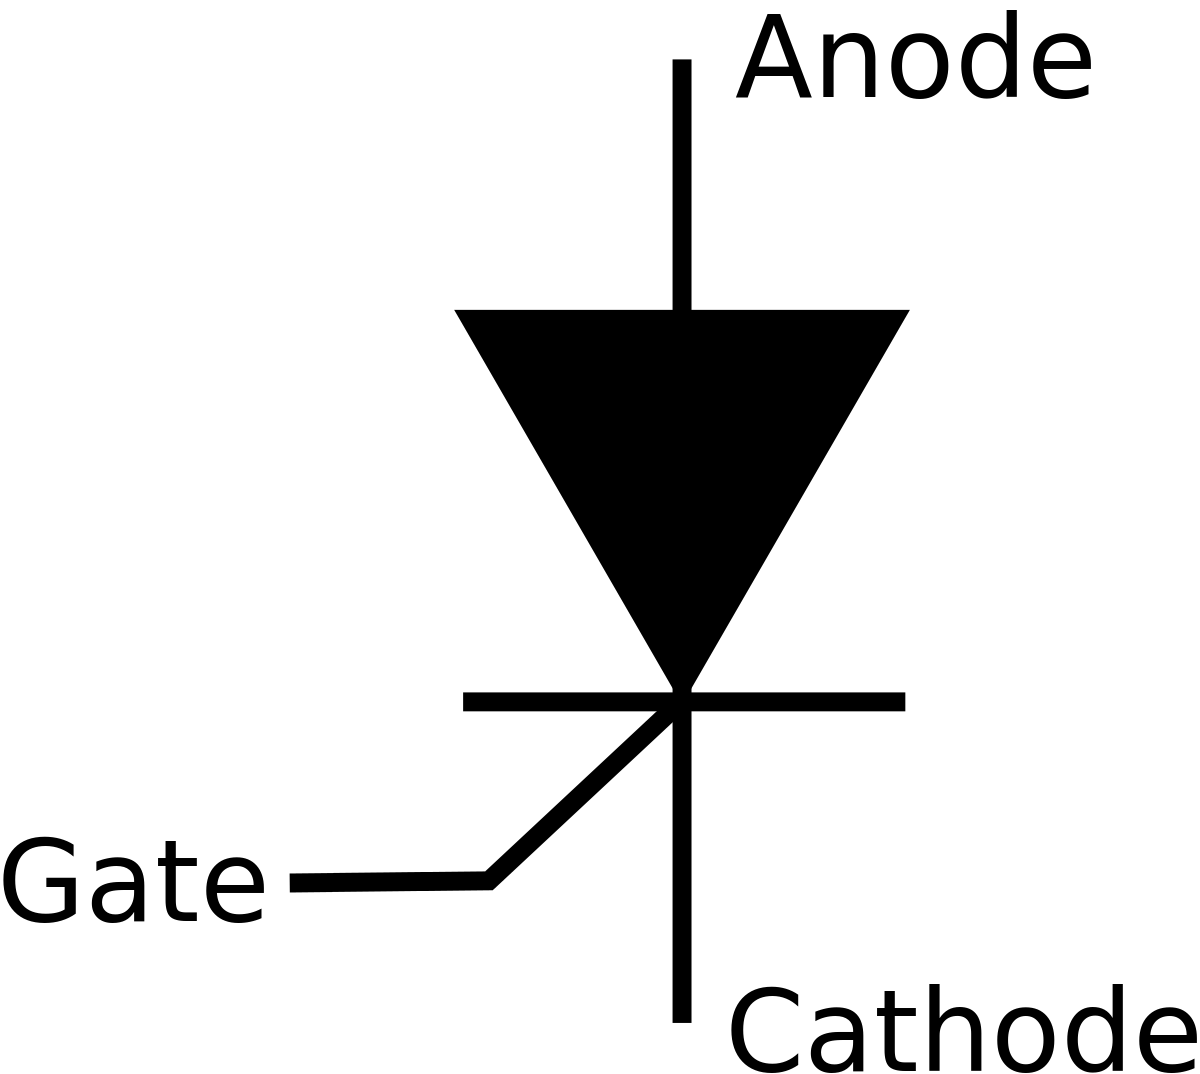
\includegraphics[width=0.5\linewidth]{Thyristor.png}
\end{figure}
\vfill

{
\renewcommand\arraystretch{2}
\begin{center}
\begin{tabular}{>{\bf}p{4cm} l}
Hochschule                 &    Hochschule für Technik - FHNW\\
Studiengang                &    Elektro- und Informationstechnik\\
Autor   		           & 	Nando Spiegel und Bastian van Dijke\\
Betreuer                   &    Felix Jenni\\
Auftraggeber               &    Intern\\
%Version                    &    1.2 %Normally not used!
\end{tabular}
\end{center}
}

\clearpage
			
%%---ABSTRACT----------------------------------------------------------------------------
\selectlanguage{ngerman}				%ngerman or english
\thispagestyle{empty}
\begin{abstract}

Heutzutage gibt es zwei einfache Verfahren für die Leistungsregelung von passiven Geräten wie Heizung und Lampen. Eine ist die Phasenanschnittsteuerung, die oft bei ohmschen Lasten verwendet wird. Bei dieser Methode treten mehrfach harmonische Schwingungen auf. Daher sind ihr vom Netzbetreiber einige Grenzen gesetzt. Die zweite Steuerungsart ist die Schwingungspaketsteuerung. Hierbei wird die Leistung während mehreren Netzperioden voll bezogen und danach wieder abgeschaltet. Dieses harte Ein- und Ausschalten des Verbrauchers erzeugt im Netz sub- und zwischenharmonische Schwingungen. Der Nachteil dieser Oberschwingungen sind, dass sie das Netz mit Blindleistung belasten. Ausserdem können Fehlverhalten bei Betriebsmitteln hervorrufen oder diese sogar zerstören.\\ 
In der vorliegenden Arbeit wurde eine dritte Variante entwickelt, um die Nachteile zu minimieren. Sie besteht aus einer Kombination der beiden Steuerungsverfahren. Dabei wird das sanfte Hoch- und Runterfahren der Leistung mit der Phasenanschnittsteuerung ausgeführt. Die Schwingungspaketsteuerung kommt zu tragen, um die Anzahl Pakete ein- und auszuschalten.\\
Es zeigte sich, dass bei der neu entwickelten Methode die harmonischen Oberschwingungen zu einem minimalen Wert absinken. Sie können so für höhere Leistungen eingesetzt werden und immer noch die Vorschriften des Netzbetreibers erfüllen. Je sanfter das Ein- und Ausschalten das heisst die Steilheit, der Leistung gewählt wurde, desto näher waren die Zwischenharmonischen bei den jeweiligen harmonischen Schwingungen im Vergleich zur Schwingungspaketsteuerung. Ausserdem waren die Seitenbänder viel schmaler als bei der Paketsteuerung. Die Auswirkungen dieser sub- und zwischenharmonischen Schwingungen konnten jedoch nicht genau analysiert werden.

 
  
   

%Bei empirischen Studien: die Charakteristika der Stichprobe, insbesondere Alter, Geschlecht, Ethnie, Patienten oder gesunde VPn etc., sowie die zentralen Aspekte der verwendeten Methoden und Prozeduren (entspricht dem Methodenteil). Besonders relevant sind solche Informationen, die wahrscheinlich bei der elektronischen Suche berüchsichtigt werden.



%die zentralen Resultate sowie, bei empirischen Studien, die statistischen Signifikanzen und/oder Effektstärken, Konfidenzintervalle u.ä. (entspricht dem Resultateteil)


%die Folgerungen, Implikationen oder Anwendungsmöglichkeiten (entspricht der Diskussion).

%die Fragestellung, wenn möglich in einem einzigen Satz (entspricht der Einführung). Oft wird davor auch knappe Hintergrundinformation zum Forschungsthema gegeben.
\vspace{2ex}
\textbf{Keywords: Phasenanschnitt, Schwingungspaket, Ohmsche Last}
\end{abstract}	



\section*{Danksagung}



%%---TABLE OF CONTENTS-------------------------------------------------------------------
\pagenumbering{Roman}		
\selectlanguage{ngerman}				%ngerman or english
\tableofcontents
\clearpage

%%---TEXT--------------------------------------------------------------------------------
\pagenumbering{arabic}
\section{Einleitung}


%Relevanz des Themas und Motivation


%Problembeschreibung


%Zielsetzung


%Methoden


%Aufbau der Bachelorarbeit

In der Leistungselektronik werden ein- und dreiphasige Thyristorsteller seit Jahren für verschiedenste Anwendungen eingesetzt. Dabei gibt es zwei beliebte Methoden, wie die Ansteuerung der Steller erfolgen kann. Die Phasenanschnitt-Steuerung ist eine geläufige Vorgehensweise, um die Leistung von ohmschen Lasten zu regulieren. Da bei dieser Steuerung jedoch harmonische Schwingungen (Vielfaches der Netzfrequenz) auftreten, sind ihnen vom Netzbetreiber einige Limiten gesetzt. Ein Beispiel dafür sind die zulässige Höchstwerten der Oberschwingungsströme bei den verschiedenen Ordnungen. Eine andere Möglichkeit, die verwendet wird, um Spannung und Strom zu regulieren, ist eine Schwingungspaket-Steuerung. Die Leistung wird dabei während mehreren Netzperioden voll bezogen und dann wieder weggeschaltet. Dieses strikte Zu- und Wegschalten des Verbrauchers vom Netz erzeugt neben den harmonischen, auch subharmonische Schwingungen (Bruchteile der Netzfrequenz). Diese Effekte sind im Netz unerwünscht, da die ordnungsmässige Funktion der Betriebsmittel beeinträchtigen und zu nicht sinus förmige Ströme und Spannungen führen.
Eine alternative Variante, die die oben genannten Probleme vermindern könnte, wäre eine Kombination der beiden Steuerungsarten. Dabei würde man mithilfe der Phasenanschnittsteuerung das sanfte Hoch- und Runterfahren der Spannung regulieren. Zusätzlich würde mit einer solchen Schwingungspaketsteuerung die Anzahl Pakete des Auf- und Absteuerns eingeschaltet werden.\\
Das Ziel dieser Bachelorarbeit ist es, ein solches Verfahren zu entwerfen und zu analysieren. Der Vergleich mit den bereits vorhandenen Steuerungsarten soll zeigen, dass eine Kombination der beiden Verfahren genutzt werden kann, um die verlustbehafteten Oberschwingungen zu minimieren. Mit einem geeigneten Messaufbau aller Varianten können die Unterschiede demonstriert werden.\\
Zunächst werden jedoch zuerst alle relevanten Informationen über die gängigen Steuerverfahren für ein- und dreiphasige Wechselspannungssteller zusammengetragen. Anschliessend sollen analytisch die harmonischen Oberschwingungen in Funktion zum Zündwinkel der Phasenanschnitt-Steuerung (ein- und dreiphasig) bestimmt werden. Auch die Harmonische in Funktion des Ein- und Ausschalt-Verhältnisses für Schwingungspaket-Steuerung sind ein wichtiger Bestandteil dieser Arbeit. Die Resultate aller Steuerungsverfahren, die man mit den Simulationstools Plecs und Matlab aufgebaut hat, werden mit einem geeigneten Laboraufbau verglichen. Danach betrachtet man ein Verfahren mit sanftem Hoch- und Runterfahren der Leistung und verifiziert die zugehörigen Simulationen mit den Messungen. Mithilfe eines Arduinos und einer kleinen Software kann schlussendlich die neu entwickelte Ansteuerung bei einer ohmschen Last und einem Asynchronmotor getestet werden. Bei den gefundenen Verfahren muss immer darauf geachtet werden, dass sie zwingend die Netzvorschriften einhalten.\\
Die vorliegende Projektarbeit gliedert sich in 5 Kapitel. Im ersten Teil werden die wichtigsten Grundlagen erläutert. Dies sind die Funktion der einzelnen behandelten Steuerungsarten, die damit auftretenden Probleme und die Formeln, die für die Berechnungen der verschiedenen Spektren, verwendet wurden. Ausserdem werden die wichtigsten Normen kurz zusammengefasst. Im Kapitel Simulation sind alle Resultate der simulierten Verfahren, welche mit Plecs und Matlab dargestellt sind, aufgezeigt. Zusätzlich wurden die Resultate der beiden Simulationsprogrammen miteinander verglichen und gegenseitig verifiziert. Das 4. Kapitel beinhaltet den Messaufbau sowie alle Komponenten, die verwendet wurden, um einen geeigneten Laboraufbau zu erstellen. Anschliessend sind im Kapitel 5 die Resultate des Messaufbaus vorgestellt. Am Ende folgt im Kapitel 6 die Diskussion zu den verschiedenen Ansteuerungsverfahren und es wird ein abschliessendes Fazit gezogen.
























\section{Grundlagen}
In diesem Kapitel werden die verschiedenen Grundlagen für die Steuerungsarten erklärt.
\subsection{Phasenanschnittsteuerung}
Bei der Phasenanschnittsteuerung wird das Sinussignal über einen TRIAC geführt. Ein TRIAC sind zwei antiparallel geführt Thyristoren. Dieser zündet ab einem gewissen Zündimpuls nach jedem Nulldurchgang. Je später der TRIAC eingeschaltet wird, desto kleiner wird die mittlere Leistung über der Last. Ein Vorteil gegenüber einem Spannungsteiler ist, dass weniger Leistung gebraucht wird. Der Zündwinkel kann von 0\textdegree bis 180\textdegree gewählt werden, wobei bei 0\textdegree die maximale Leistung und bei 180\textdegree keine Leistung über der Last anliegt. Das Problem bei der Phasenanschnittsteuerung ist, dass diese Schaltung Oberwellen verursacht und so ungewünschte Effekte für den Netzbetreiber verursacht. Ein weiteres Problem betrifft den nicht-sinusförmigen Stromverlauf. Da Strom und Spannung nicht den gleichen Verlauf haben, tritt eine Verzerrungsblindleistung auf.  Der Strom verläuft zeitlich der Spannung nach wirkt so wie eine Induktivität. Deshalb wird dieses Verfahren vom EW nur bei kleinen Leistungen toleriert. Bei grossen Leistungen wird deshalb die Schwinungspaketsteuerung benutzt. In der Abbildung \ref{fig:Phasenanschnitt} ist erischtlich, wie der Phasenanschnitt bei einer Netzspannung aussieht. Grau gezeichnet ist die normale Netzspannung und rot ist die Spannung welcher an der Last anliegt. In dieser Abbildung wurde ein Winkel von 135\textdegree gewählt und somit ist die Leistung an der Last kleiner als mit der normalen Netzspannung. 

\begin{figure}[ht!]
	\centering
	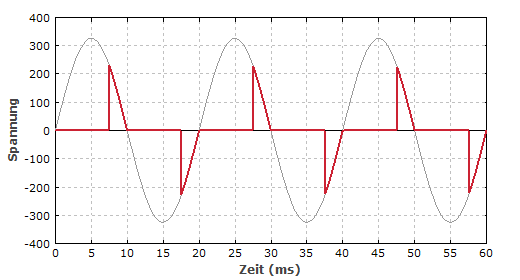
\includegraphics[scale=0.75]{phasenanschnittsteuerung1.png}	
	\caption{Phasenanschnitt mit einem Winkel von 135\textdegree \cite{Phasenanschnittsteuerung}}\label{fig:Phasenanschnitt1}
\end{figure}
\newpage
\begin{figure}[ht!]
	\centering
	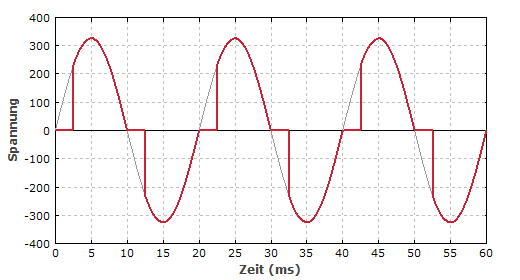
\includegraphics[scale=0.75]{phasenanschnittsteuerung2.png}	
	\caption{Phasenanschnitt mit einem Winkel von 45\textdegree \cite{Phasenanschnittsteuerung}}\label{fig:Phasenanschnitt2}
\end{figure}
Bei der Abbildung \ref{fig:Phasenanschnitt2} ist gut ersichtlich, wie früher gezündet wurde. Somit wird die Leistung an der Last grösser.

\subsection{Schwingungspaketsteuerung}
In diesem Verfahren wird nicht wie der Phasenanschnittsteuerung die Form der Halbwellen verändert, sondern die Zeitdauer. Dabei wird immer von der Paketzeit und der Einschaltzeit ausgegangen, wobei letzteres verändert wird. Wenn z.B. eine Paketdauer 10 Halbwellen hat, und die Einschaltdauer 5 Halbwellen ist, liegt die halbe Leistung über der Last an. Anders als bei der Phasenanschnittsteuerung enstehen bei dieser Ansteuerungsart keine harmonische Oberwellen, dafür aber Sub- und Zwischenharmonische. Auf der Abbildung \ref{fig:Schwingungspaketsteuerung} ist ersichtlicht, wie vier von den total sechs pro Paket eingeschaltet sind. Dies ergibt eine Leistung welche ${2}/{3}$ so gross ist wie die Leistung mit der normalen Netzspannung.

\begin{figure}[ht!]
	\centering
	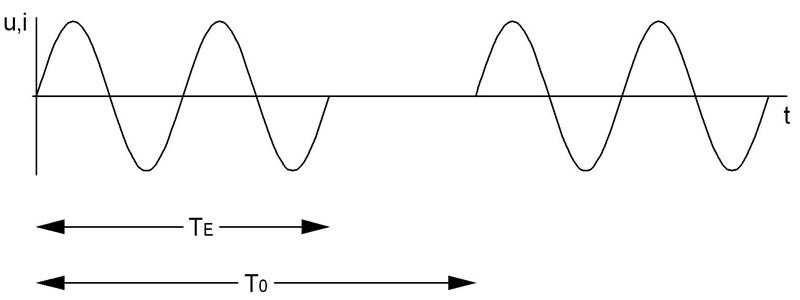
\includegraphics[scale=0.5]{Schwingungspaketsteuerung.png}	
	\caption{Schwingungspaketsteuerung ${2}/{3}$ der Leistung \cite{Schwingungspaketsteuerung}}\label{fig:Schwingungspaketsteuerung}
\end{figure}

Dabei ergibt sich aus dem Verhältnis von Einschaltdauer zu Periodendauer das Tastverhältnis.

\begin{equation}\label{eq:Einschaltverhältnis}
a = \frac{T_E}{T_0}
\end{equation}

\subsection{TRIAC}
Der TRIAC beseht aus zwei anti-parallele Thyristoren und kann über das Gate gezündet werden. Der TRIAC bleibt solange leitend bis der Haltestrom unterschritten wird. 

\begin{figure}[ht!]
	\centering
	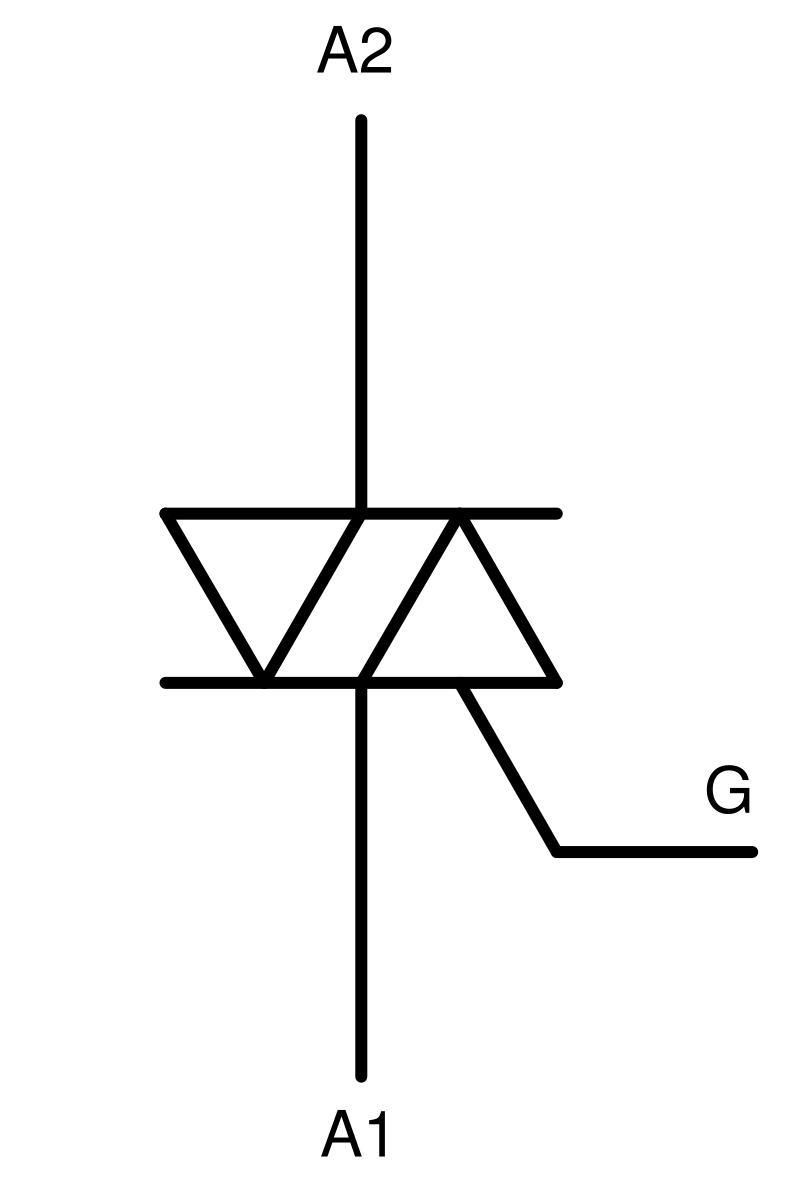
\includegraphics[scale=0.1]{TRIAC.png}	
	\caption{Schaltzeichen eines TRIACs \cite{TRIAC}}\label{fig:TRIAC}
\end{figure}




\subsection{Leistungsfaktor}
Bei beiden Verfahren ist der Leistungsfaktor vom Zündwinkel oder dem Einschaltverhältnis abhängig. 

In der Abbildung \ref{fig:Leistungsfaktor} ist ersichtlich wie der Leistungsfaktor bei den beiden Steuerungsarten aussieht. Bei der Phasenanschnittsteuerung auf der linken Seite sieht man, wie bei einem kleinem Zündwinkel der Leistungsfaktor sehr gross ist. Je grösser der Zündwinkel gewählt wird, desto kleiner wird der Leistungsfaktor. Auf der rechten Seite sieht man den Leistungsfaktor in Abhängigkeit des Einschaltverhältnisses. Je grösser das Einschaltzeitverhältnis, desto grösser der Leistungsfaktor.  
\begin{figure}[ht!]
	\centering
	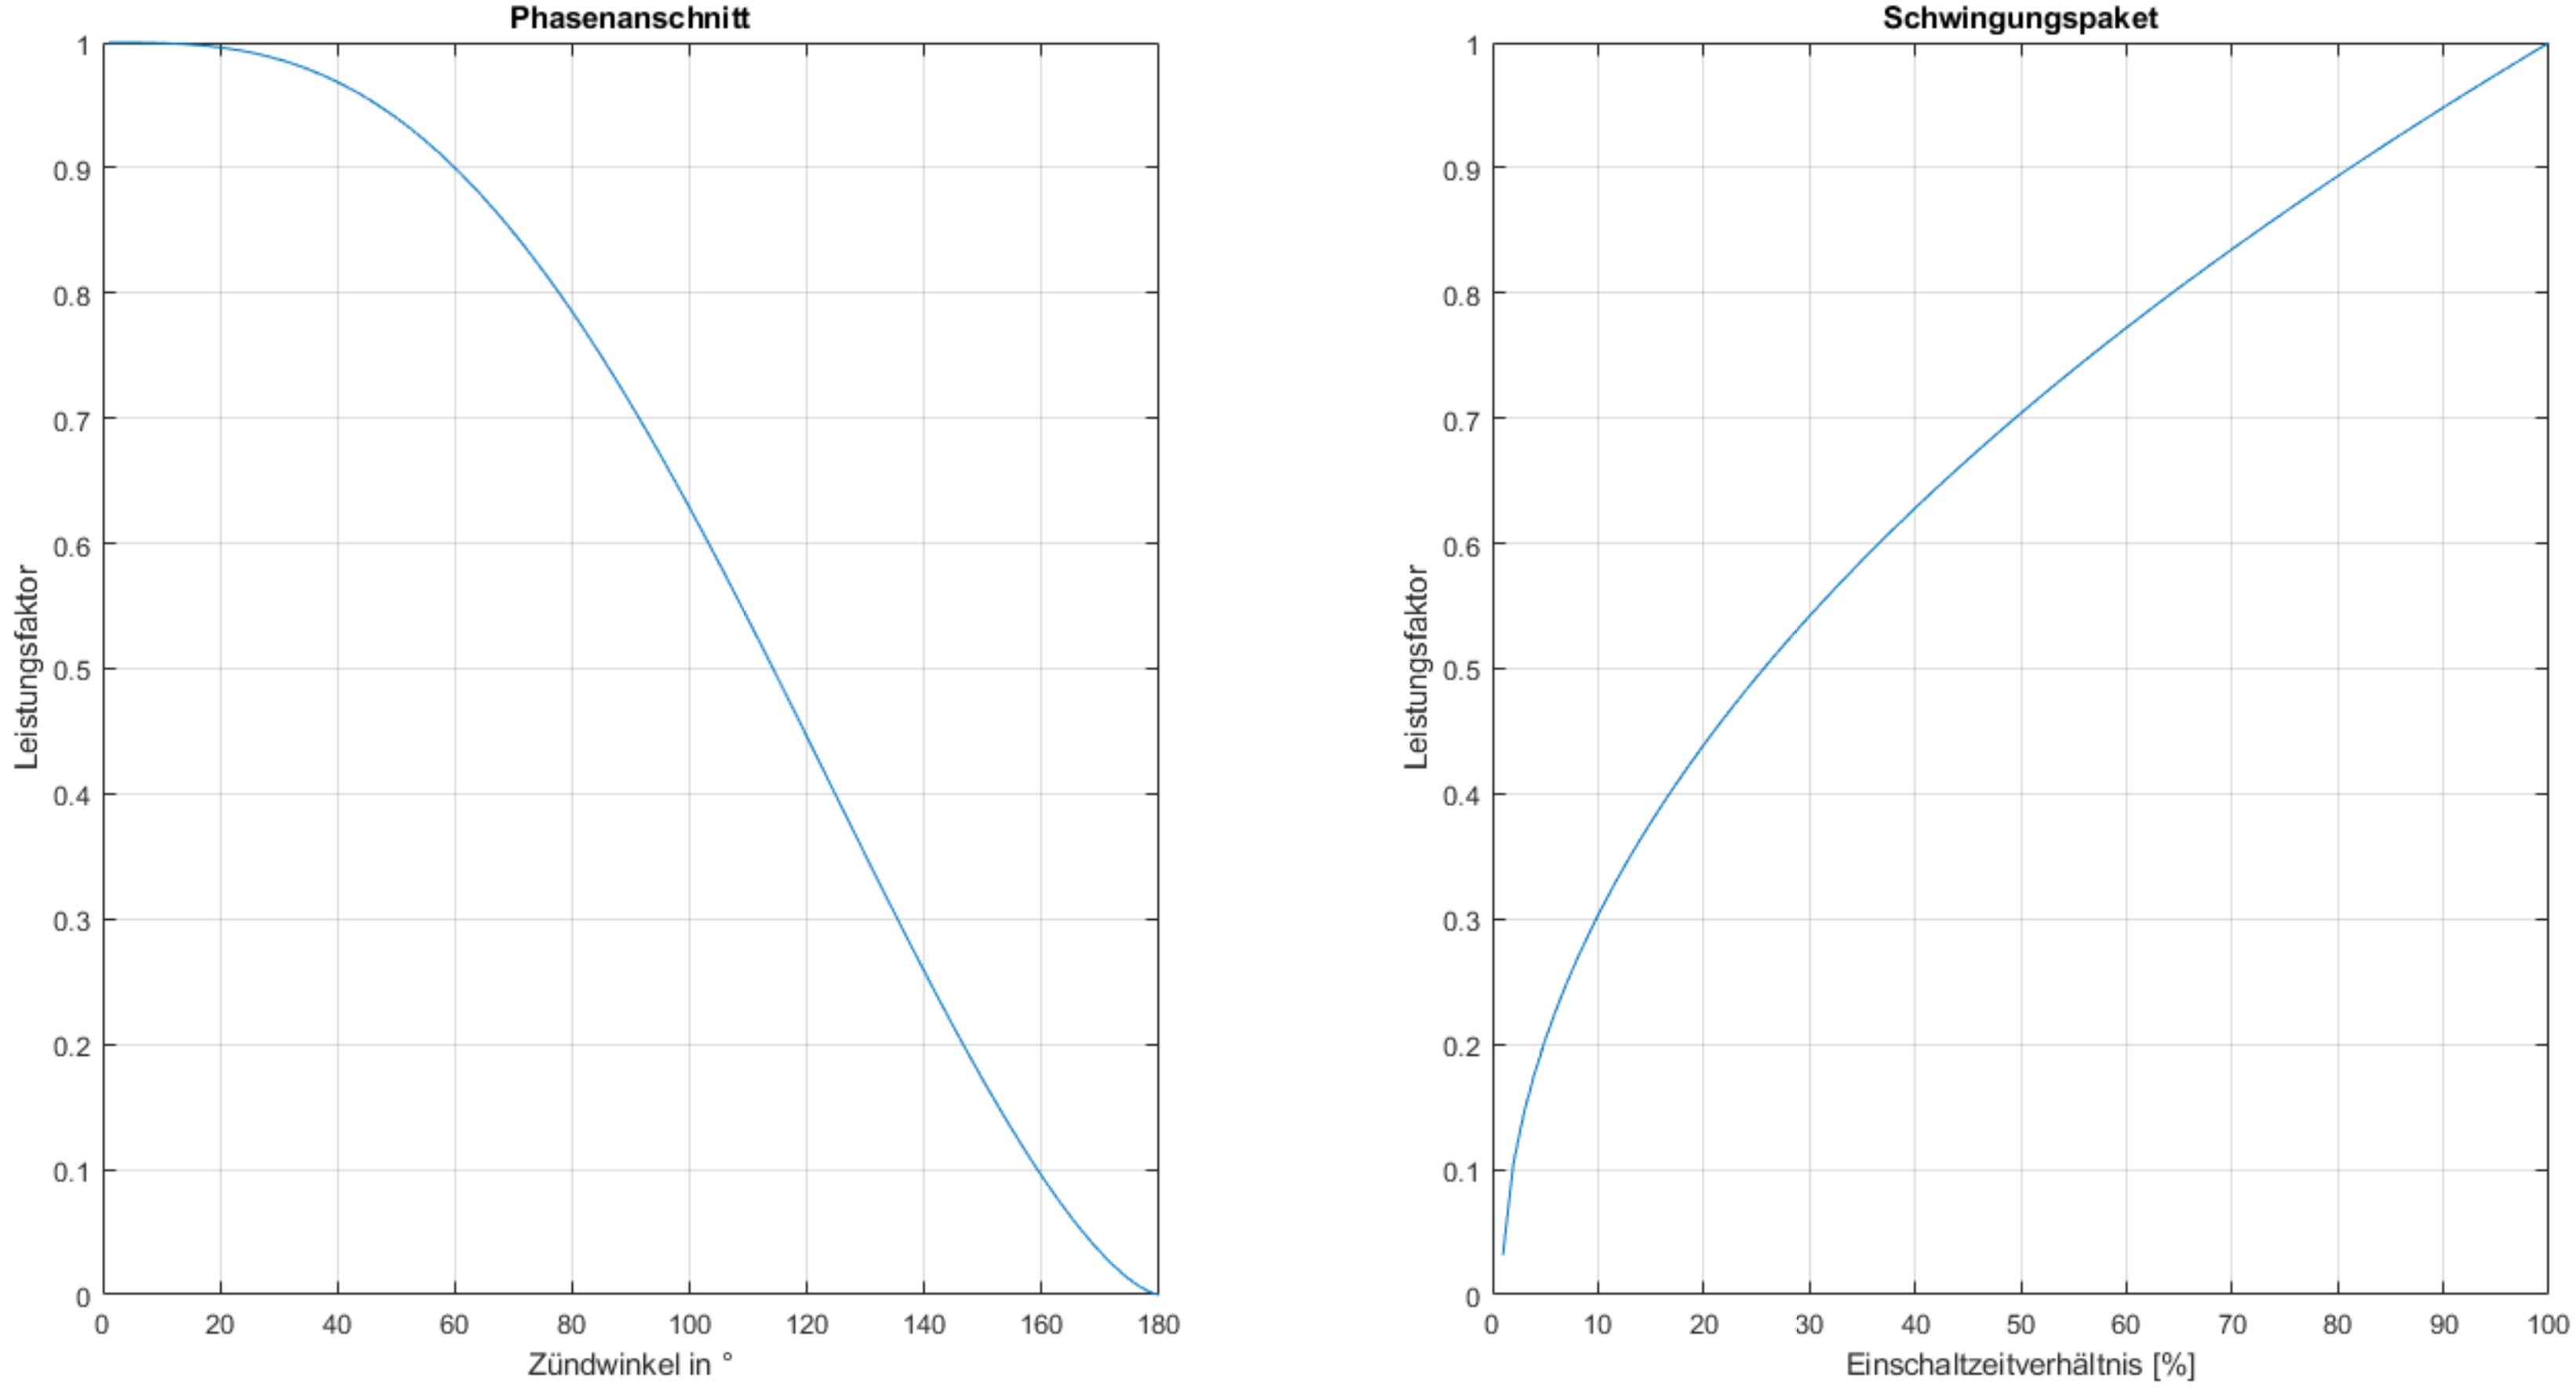
\includegraphics[scale=0.394]{Leistungsfaktor.png}	
	\caption{Leistungsfaktor von Phasenanschnitt- und Schwingungspaketsteuerung}\label{fig:Leistungsfaktor}
\end{figure}

\subsubsection{Leistungsfaktor Phasenanschnittsteuerung}
Der Leistungsfaktor ist definiert als das Verhältnis von Wirkleistung zu Scheinleistung. 
\begin{equation}\label{eq:lamda_p}
\lambda = \frac{P_{\alpha}}{S}
\end{equation}
Die Schein- und Wirkleistung können mit den folgenden Formeln beschrieben werden.
\begin{equation}\label{eq:Schein-&Wirkleistung}
\begin{array}{cc} 
S = I_L \cdot U_{UN}   &   P_{\alpha} = I_L^2 \cdot R_L  \\
\end{array}
\end{equation}
Werden die Formeln \ref{eq:Schein-&Wirkleistung} in die Formel \ref{eq:lamda_p} eingesetzt ergibt sich folgende Gleichung. 
\begin{equation} \label{eq:Phas_1}
\frac{P_{\alpha}}{S} = \frac{I_L \cdot R_L}{U_{UN}}
\end{equation}
Der Laststrom wird mit folgender Formel beschrieben.
\begin{equation}
I_L = \sqrt{1-\frac{\alpha}{\pi}+\frac{1}{2\pi} \cdot sin(2\alpha)} \cdot \frac{U_{UN}}{R_L}
\end{equation}
Wenn die Formel für den Laststrom in die Gleichung \ref{eq:Phas_1} eingesetzt wird, lassen sich die Spannung und der Widerstand wegkürzen und übrig bleibt folgende Formel.
\begin{equation}
\lambda = \sqrt{1-\frac{\alpha}{\pi}+\frac{1}{2\pi} \cdot sin(2\alpha)}
\end{equation}

\subsubsection{Leistungsfaktor Schwingungspaketsteuerung}
Das Einschaltsverhältnis wird mit $a$ beschrieben und wird mit der Formel \ref{eq:Einschaltverhältnis} beschrieben.
Die Schein- und Wirkleistung werden mit den folgenden Formeln beschrieben.
\begin{equation}\label{eq:Schw_Schein-&Wirkleistung}
\begin{array}{cc} 
S_a = \sqrt{a} \cdot P  &   P_a = a \cdot P \\
\end{array}
\end{equation} 
Wenn die beiden Formeln für die Wirk-und Scheinleistung in die Gleichung für den Leistungsfaktor eingesetzt wird ergibt sich daraus folgende Gleichung.  
\begin{equation}
\lambda = \frac{P_a }{S_a} = \frac{a \cdot P}{\sqrt{a} \cdot P}
\end{equation}
Die Wirkleistung lässt sich wegkürzen und so ergibt sich folgende Formel.
\begin{equation}
\lambda = \sqrt{a}
\end{equation}

\subsection{Oberschwingungen}
Im Idealfall würde bei einer Stromversorgung überall eine perfekte sinusförmige Spannung vorliegen. Jedoch sieht dies in der Realität anders aus. Die Kurve der Spannung und des Stromes weichen massiv von einer Sinusfunktion ab. Man bezeichnet diese verzerrten Schwingungsformen im Allgemeinen als oberschwingungsbehaftetes Signal. 

Schon früh erkannte man diese Oberschwingungsverzerrungen am Netz, jedoch ist es erst heute ein ernstzunehmendes Problem für die Versorgungsbetriebe, die Verteilnetzbetreiber und für den Endkunden. Früher waren die grössten Herausforderungen, die Auswirkungen von Oberschwingungsverzerrungen auf elektrische Maschinen zu erkennen. Man stellte ausserdem fest, dass Störungen in den Telefonleitungen auftraten, welche den Ton der Sprache beeinträchtigte. Allerdings kann man sagen, dass Oberschwingungsverzerrungen früher ein geringeres Gefahrenpotential darstellten als heute. Die heutigen Maschinen wurden neuerdings so konstruiert, dass sie weniger Oberwellen erzeugen. Auch bei den Verteilnetzen wurde darauf geachtet, dass sie nicht mehr an der Lastobergrenze arbeiten und so ein reineres Sinussignal verwenden. Seit einigen Jahren steigt, die weltweite Nachfrage nach energieeffizienten Lösungen, die nur über vermehrten Einsatz von Leistungselektronik realisierbar sind. 
\subsection{Grundlagen}
Die Bedeutung Oberschwingung kommt aus dem Themenbereich «physische Eigenwertprobleme» also Wellen, deren Frequenz ganzzahlige Vielfache der Grundschwingungen sind. In der Musikwelt kann man Oberschwingungsfrequenzen vor allem bei Saiteninstrumenten, wie zum Beispiel bei einer Gitarre oder einer Geige beobachten.\\
Die meisten elektrischen Geräte halten sich nach der perfekten Welle Ausschau. Bei Wechselstrom definiert die Perfektion einen perfekte Sinuskurve. Die daraus verwendete elektrische Spannung wechselt gleichmässig zwischen der positiven un negativen Halbwelle hin und her. Bei einer Frequenz von 50 Hz beträgt dies genau 50-mal pro Sekunde. Der Begriff Welle ist mit dem Zusammenhang von Oberschwingungen nicht ganz korrekt. Eine Welle hat eine räumliche und zeitliche Ausdehnung, jedoch haben die hier betrachteten Schwingungen nur eine zeitliche Ausdehnung. Die Oberschwingungsanteile in einem Wechselstromsystem sind also definiert als sinusförmige Anteile einer periodischen Schwingung, deren Frequenz einem ganzzahligen Vielfachen (Ordnungszahl) der Grundfrequenz entspricht. In der unteren Tabelle erkennt man, welche Ordnungszahl $(n)$  zu welcher Frequenz $(fh)$ gehört. Es ist ersichtlich, dass zum Beispiel die 5. Oberschwingung eine Frequenz von 250 Hz hat. Die Berechnung der Oberschwingungsfrequenz ist in der unterstehenden Formel \ref{eq:Oberschwingungsfrequenz} dargestellt.

\begin{equation}\label{eq:Oberschwingungsfrequenz}
f_h = n \cdot Grundfrequenz
\end{equation}

\begin{table}[ht!]
	
	\centering
	
	\begin{tabular}{|l|l|}
		
		\hline
		
		\begin{tabular}[c]{@{}l@{}}Ordnungszahl\\   $n$\end{tabular} & \begin{tabular}[c]{@{}l@{}}Oberschwingungs-\\frequenz (Hz)  $f_h$\end{tabular} \\ \hline
		
		1                                                            & 50                                                              \\ \hline
		
		3                                                            & 150                                                             \\ \hline
		
		5                                                            & 250                                                             \\ \hline
		
		7                                                            & 350                                                             \\ \hline
		
		11                                                           & 550                                                             \\ \hline
		
		13                                                           & 650                                                             \\ \hline
		
		…                                                            & …                                                               \\ \hline
		
		n                                                            & 50*n                                                            \\ \hline
		
	\end{tabular}
	
	\caption{Oberschwingungsfrequenzen}\label{tab:Oberschwingungfrequenz}
	
\end{table}

\begin{figure}[ht!]
	\begin{minipage}[t]{0.49\textwidth}
		\centering
		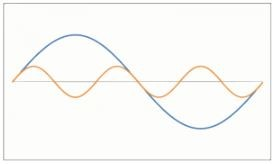
\includegraphics[scale=2]{Schwing_3.jpg}	
		\caption{Grundschwingung mit 3. Ordnung \cite{Oberwellen}}\label{fig:Schwing3}
	\end{minipage}	
		%
	\begin{minipage}[t]{0.49\textwidth}	
		\centering	
		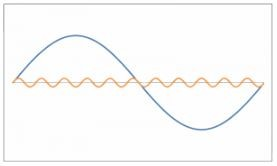
\includegraphics[scale=2]{Schwing_11.jpg}	
		\caption{Grundschwingung mit 11. Ordnung \cite{Oberwellen}}\label{fig:Schwing11}
	\end{minipage}
\end{figure}
	
Die folgenden zwei Abbildungen \ref{fig:Schwing3} \& \ref{fig:Schwing11} zeigen eine Grundschwingung bei 50 Hz (blau) und die jeweilige 3. und 11. Ordnung der Grundfrequenz (gelb).

\subsection{Verzerrte Schwingung}
Eine verzerrte Schwingung entsteht durch Überlagerungen von verschiedenen sinusförmigen Wellen mit unterschiedlichen Frequenzen und Amplituden. Man kann eine solche Schwingung mit unterschiedlichen Oberschwingungskomponenten, auch Komposition genannt, zusammensetzen, indem man eine Sinusschwingung mit mehreren Oberschwingungen zusammenaddiert. Das folgende wellenförmige verzerrte Signal lässt sich zu einer Grundschwingung mit ihren mehreren harmonischen Oberschwingungen zerlegen. Bei der untenstehenden Graphik \ref{fig:Addition Oberwellen} ist diese ersichtlich, wobei die rote Kurve das verzerrte Signal ist. Die blauen Sinusschwingungen sind die Zerlegungen in die Grundschwingung der 3. und 5. harmonische Oberschwingung. Addiert man wiederum die drei blauen Kurven miteinander erhält man das verzerrte rote Signal.   

\begin{figure}[ht!]
	\centering
	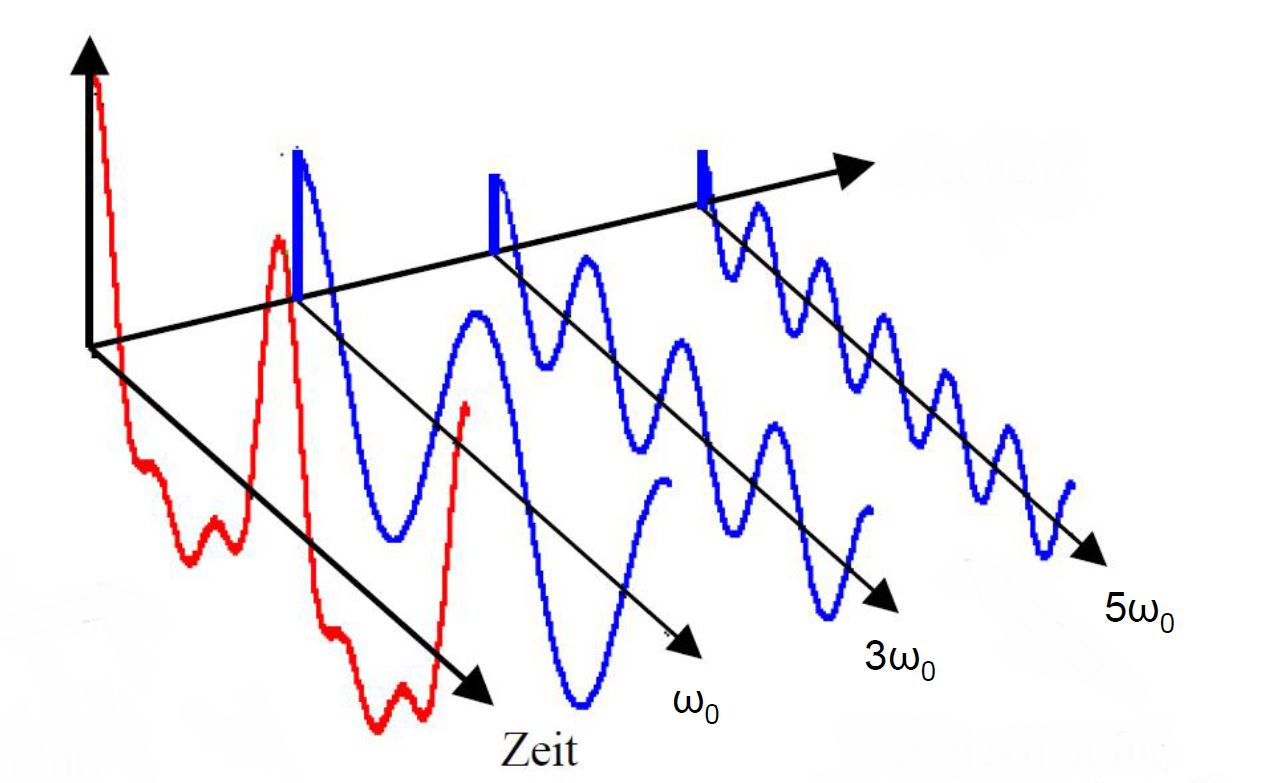
\includegraphics[scale=0.7]{verzerrtes_Signal_analysis.png}	
	\caption{Addition der verschiedenen Oberwellen \cite{analysi3}}\label{fig:Addition Oberwellen}
\end{figure}


Die erste Person, welcher diese Methode vorgestellt hat, war der französische Mathematiker Jean Baptiste Fourier. Noch heute trägt die Fourier-Transformation diese Bezeichnung. Mit diesem Zusammenhang kann die Überlagerung von einer perfekten Sinuskurve zu einer verzerrten Sinusschwingung führen. Dies Bedeutet so viel wie, eine verzerrte Sinusschwingung lässt sich immer als Überlagerung einer Grundschwingung mit anderen Oberschwingungen unterschiedlicher Frequenzen und unterschiedlichen Amplituden darstellen. Anhand eines Amplitudenspektrums lassen sich die Oberschwingungen gut visualisieren. 
\todo {evt. noch Bild mit Amplitudenspektrum einfügen}
Bei den Oberschwingungen gibt es ungerade oder gerade harmonische Schwingungen.
Die ungeraden Oberwellen sind die charakteristischen Oberschwingungsanteile in den heutigen Stromversorgungsnetzen. Sie stellen Wellenformen dar, die bezogen auf die Zeitachse symmetrisch sind. Aufgrund der meist dreiphasigen Symmetrie der heutigen Infrastrukturen sind nahezu alle Signale symmetrisch, obwohl es zu Verzerrung kommt. Geradzahlige Oberschwingungen können nur aus Wellenformen entstehen, die nicht symmetrisch bezogen auf die Zeitachse sind.

\subsection{Vorkommen der Oberschwingungen}
Oberschwingungsströme erzeuget fast jedes elektrische Gerät. Doch welches Gerät welche Stromverzerrung erzeugt wird später erklärt. Ein wichtiger Bezugspunkt zu den individuellen Oberschwingungsgrössen ist die gesamte harmonische Verzerrung. Man nennt ihn auch den THD-Wert (Total Harmonic Distortion). Diesen Wert gilt es besonders zu verstehen, damit man ihn rechnerisch analysieren kann. Er gibt das Verhältnis des Effektivwertes aller Oberschwingungen zum Effektivwert der Grundschwingung an. Man verwendet ihn üblicherweise im Nieder-, Mittel-, aber auch im Hochspannungsnetz. Normalerweise wird die Verzerrung des Stromes als THDi, beschrieben in der Formel \ref{eq:THDi} und die Verzerrung der Spannung als THDu, ersichtlich in der Formel \ref{eq:THDu} angegeben. Der Total Harmonic Current (THC) ist der gesamte Oberschwingungsstrom. Er wird verwendet, um den Gesamteffektivwert der Oberschwingungsströme der Ordnung 2 bis 40 zu quantifizieren, die zu einer Verzerrung der Stromkurve beitragen. Man erkennt dies in der Formel \ref{eq:THC}. Diesen Wert braucht man vor allem, um die erforderlichen Eigenschaften zur Auswahl eines effizienten aktiven Oberschwingungsfilters zu bestimmen.
Bei der folgenden Formel handelt es sich um den Gesamten Oberschwingungsstrom.
\begin{equation}\label{eq:THC}
THC = {\sqrt{\sum_{n=2}^{40} I_n^2}}
\end{equation}



Die gesamte harmonische Verzerrung des Stromes gibt, wie der Name schon sagt, die gesamte Verzerrung des Stromes an. Der Wert ist definiert als Quotient des Effektivwerts der Oberschwingungsströme im Verhältnis zum Grundschwingungsstrom. Typischerweise wird die Summe aller Stromoberschwingungsanteile in Bezug auf den Grundschwingungsstrom bis einschliesslich der 40. Oberschwingung berechnet. Die Oberschwingungsströme, welche durch Lasten in Netzwerken erzeugt werden, müssen durch die Impedanzen der Transformatoren oder Drosseln fliessen. An diesen Impedanzen kommt es zu nichtlinearen Spannungsabfällen. Es werden Oberschwingungsspannungen erzeugt die im ganzen Netz verbreitet werden. Diese können an Endgeräten eine Verzerrung der Versorgungsspannung verursachen. Somit ist die harmonische Verzerrung des Stromes (THDi) eine direkte Ursache für die Verzerrung der Spannung (THDu = Total Harmonic Distortion of Voltage). Sie gibt das Ausmass der Verzerrung der Versorgungsspannung an. Auch dieser Wert ist definiert als Quotient des Effektivwertes der Spannungsoberschwingungsanteile bis zur 40. Oberschwingung bezogen auf den Effektivwert der Grundschwingung. 
Folgende Formel zeigt wie man die Totale Verzerrung des Stromes in Prozent berechnet ist.
\begin{equation}\label{eq:THDi}
THDi = \frac{\sqrt{\sum_{n=2}^{40} I_n^2}}{I_{(1)}} * 100 \%
\end{equation}

Parallel dazu zeigt die untere Formel die Totale Verzerrung der Spannung in Prozent.
\begin{equation}\label{eq:THDu}
	THDu = \frac{\sqrt{\sum_{n=2}^{40} U_n^2}}{U_{(1)}} * 100\%
\end{equation}






Je niedriger der THDu-Wert ist, desto besser ist die Spannungsqualität. Die Norm besagt, dass der gesamte Oberschwingungsgehalt den Wert von 8\% nicht überschreiten darf. Dazu kommt, dass heute üblicherweise für die Verzerrung die THD-Werte angegeben sind und nicht wie früher die Oberschwingungsgehalte (Klirrfaktore).

Wenn man sich mit den Oberschwingungsproblematik befasst, ist es wichtig, den Zusammenhang zwischen Strom und Spannung zu verstehen. Dadurch ist es möglich eine geeignete Lösung für das reduzieren von Oberschwingungen zu finden. 
Je nach Eigenschaft der Oberschwingungserzeuger und der Eigenschaft eines Gerätes am elektrischen Netz, verbreiten sich Oberschwingungsströme in einem System unterschiedlich. Verschiedene Spannungsverzerrungen sind die Folgen. 

\subsection{Auswirkung von Oberschwingungen}

Falls Oberschwingungen oder andere Netzrückwirkungen bei Betriebsmitteln auftreten, können die Funktionen von den Geräten beeinträchtigt oder sogar zerstört werden. Ein Beispiel dafür wäre, im Falle einer Kurzzeitunterberechnung bei Schaltnetzteile, würden sie mit extrem hohen Einschaltspitzen reagieren. Diese Spitzen könnten das 20-fache der Nennlast erreichen. Im einphasigen Verbrauch in einem Dreiphasigen-Wechselstromsystem fliesst der ganze Rückleitstrom über den Sternpunkt des Transformators zurück. Gäbe es viele Schaltnetzteile in einem System, würden sich die Rückleiterströme nicht mehr aufheben, sondern sie würden sich addieren. Die Folgen davon wäre eine Sternpunktverschiebung. Oberschwingungen können bei Glühbirnen die Glühfadentemperatur erhöhen und somit die Lebensdauer verkürzen. Auch bei Dreh- oder Wechselstrommotoren und -generatoren führen Stromoberschwingungen zu zusätzlicher Erwärmung. Bei Schutzgeräten wie Distanzschutz, Überstromschutz oder Differentialschutz können Oberschwingungen den Aufbau und die Wirkungswiese des Schutzgerätes beeinflussen. Sind die Abstände zwischen Freileitungen und Telefonleitungen zu gering, können die Oberschwingungen die Sprachübertragung stören. Dabei gibt es vor allem ein Auge auf die 20. bis zur 30. Ordnung der Oberschwingung zu werfen.

\subsection{Anforderung an die Netzqualität}

Um die Anforderungen der Netzqualität zu gewährleisten müssen die Normen eingehalten werden. Auf welche Nomen bei dieser Arbeit genau geachtete wurde, wird zu einem späteren Zeitpunkt erläutert. Zweck der Normen sind es  die verschiedene Merkmale wie zum Beispiel Frequenz, Höhe, Kurvenform oder die Symmetrie der drei Leiterspannungen einzuhalten. Durch Lastspannung, Störeinflüsse von bestimmten Anlagen oder Auftreten von Fehlern können diese Merkmale während des Normalbetriebes des Netzes geändert werden. 


\subsection{Gegenmassnahmen bei Oberschwingungen}

Es kann durchaus vorkommen, dass in der Praxis harmonische Oberschwingungen festgestellt wurden, welche die zulässigen Grenzwerte überschreiten. Es gibt jedoch Möglichkeiten diese zu verhindern und so die Netzqualität zu verbessern. Im folgenden Abschnitt werden auf ein paar Varianten eingegangen.

\subsubsection{Vermeidung von Störungen}
Das Vermeiden von Störungen ist die einfachste Art um eine Verbesserung der Netzqualität sicher zu stellen. Der Gesetzgeber liefert dafür Normen der Elektromagnetischen Verträglichkeit, welche den gesetzlichen Grundlagen entsprechen. Sie sind zwingend einzuhalten.
\subsubsection{Stromnetzeigenschaften}
Könnte man die Netzimpedanz verringern wäre eine Reduktion der Oberschwingungen möglich. Dies ist jedoch generell nicht umsetzbar und somit kann man Kurzschlussleistung des Netzes nicht beliebig erhöhen. Die wirtschaftlichen und technischen Grenzen sind hierzu massgebend.  


\subsubsection{Oberschwingungsfilter}

Zur Begrenzung von Oberschwingungen werden heutzutage  meistens mehrere aufeinander abgestimmte passive Filter eingesetzt. Das einsetzten von den Filtern muss jedoch für jede konkrete Installation neu erstellt werden, um eine Verbesserung des Netzrückwirkungsverhaltens zu erhalten.\\
Die Industrie entwickelte wegen diesem Problem aktive Oberschwingungsfilter. Sie können sich, auch bei späteren Erweiterungen der Installation, an die neu Situation anpassen und müssen nicht ersetzt werden. Ein weiterer Vorteil dieser Flexibilität des Filters ist es, dass die Nenngrösse einfach vom aktuellen Bedarf gewählt werden kann.     

\subsubsection{Änderung der Energieversorgung}

Stark nichtlineare Betriebsmittel und empfindliche Verbraucher die zusammen an einer Gruppe angeschlossen sind, können aufgetrennt und an separate Gruppen über jeweils einen separaten Transformator eingespeist werden. Eine solche Änderung der Energieversorgung sollte aber auch immer unter wirtschaftlichen Gesichtspunkten betrachtet werden.

\subsubsection{EMV verträgliche Gebäudeinstallation}

Um Schäden durch Oberschwingungen zu vermeiden müssen bei Gebäuden die Installation EMV-verträglich sein.
Folgende Punkte sollten dabei zwingend beachtet werden:

\begin{itemize}
	\item Es sollte ein konsequentes TN-S-Netz mit getrenntem Neutral- und Schutzleiter aufgebaut werden. Die beiden Leiter sollten nur eine Verbindung zwischen einem Punkt haben.
	\item Um Schäden an einer Anlage zu vermeiden wäre ein Überspannungsschutz für Kompensationsanlagen von Vorteil.
	\item Wie schon erwähnt, wären getrennte Stromkreisgruppen für allgemeine und IT-Betriebs-mittel vorteilhaft.
	\item Leitende oder metallene Teile, wie zum Beispiel Trasse, Rohre oder Lüftungskanäle sollten zwingend mit dem Potentialausgleich verbunden werden.
	
\end{itemize}

Auch die Energieversorgung bei der Gebäudeinstallation sollte EMV-verträglich sein. Folgende Punkte sollten dabei eingehalten werden. 

\begin{itemize}
	\item Das Erdungssystem sollte niederohmig und stromfähig installiert sein.
	\item Im Schutzleiter- und Potenzialausgleich-Systeme sollten keine Arbeitsströme zugelassen sein.
	\item Bei Mehrfacheinspeisung dürfen keine Mehrfacherdung des Neutralleiters zugelassen werden.
	\item Der Kabelquerschnitt sollte für die Oberschwingungen ausgelasstet sein.
\end{itemize}  


\subsubsection{Subharmonische}
Da nicht nur harmonische Oberwellen verglichen werden, werden hier noch die Subharmonische erklärt und was der Unterschied zu den harmonischen Oberwellen ist. 
\subsubsection{Fast Fourier Transformation}
Damit die beiden Spektren der Oberwellen verglichen werden können, wird diese in einem FFT Diagram aufgezeigt. Wie diese zu lesen sind und was sie aussagen, wird hier beschrieben. 


\subsection{Normen}
Im folgenden Text werden auf alle Normen eingegangen, welche für diese Arbeit als wichtig empfunden wurde. Es sind dies vor allem Normen für die Elektromagnetische Verträglichkeit. Dazu gehören auch die Grenzwerte der Oberschwingungsströme, die Begrenzung von Spannungsänderungen, Spannungsschwankungen in öffentlichen Niederspannungsnetzen...


\subsubsection{EN 61000-3-2}
Bei dieser Norm handelt es sich um Grenzwerte für Oberschwingungsströme von (Geräten mit einem Eingangsstrom $ \leq\ $  16 A je Leiter)
Der Zweck dieser Norm ist es, die Grenzwerte für Oberschwingungen von Geräten festzulegen, die in den Anwendungsbereich dieser Norm fallen. Es sollte sichergestellt werden, dass unter Berücksichtigung der Aussendungen anderer Geräte bei Übereinstimmung mit den Grenzwerten, die Oberschwingungs-Störpegel nicht die festgelegten Verträglichkeitspegel überschreiten. Falls Geräte diese Anforderungen der Norm nicht erfüllen, kann der Anschluss an bestimmten Arten ans Niederspannungsnetz gleichwohl erlaubt werden, dann wenn die Bedienungsanleitung eine Anforderung enthält, dass das jeweils zuständige Energieversorgungsunternehmen nach einer Anschlussgenehmigung gefragt werden muss.  

\subsubsection*{Anwendungsbereich}
Dieser Teil gilt für die Begrenzung der Oberschwingungsströmen, die in das öffentliche Niederspannungsnetz eingespeist werden. Ausserdem legen sie die Grenzwerte der Oberschwingungsanteile des Eingansstromes fest , die durch ein Gerät hervorgerufen werden Können, das unter festgelegten Bedingungen geprüft wird.
Die Oberschwingungsanteile wie im Anhang A gezeigt gemessen.
Die Prüfbedingung für die Messung von Oberschwingungsströme sind für die verwendeten Geräten in Anhang C angegeben.

\subsubsection*{Klassifizierung von Geräten}

Um zu unterscheiden welche Betriebsmittel welche Oberschwingungsströme zu Begrenzen haben, wurden die Geräte in vier verschiedene Klassen von A bis D unterteilt. Da es sich bei dem Projekt um ein symmetrische, dreiphasige, ohmsche Last handelt fällt dies unter die Klasse A. Dazu kommen folgende Einrichtungen die die Klasse A auch noch beinhaltet:
\begin{itemize}
\item Haushaltsgeräte, ausgenommen Geräte, die in die Klasse D fallen
\item Elektrowerkzeuge, ausgenommen tragbare Elektrowerkzeuge
\item Beleuchtungsregler
\item Audio-Einrichtung
\end{itemize} 

Die weiteren drei Klassen werden hier nicht weiter aufgezählt, da sie für die Projektarbeit nicht relevant sind. Ausserdem fallen alle Geräte die nicht speziell aufgelistet sind sowieso in die Klasse A.

\subsubsection*{Allgemeine Anforderung}
Alle Anforderungen und Grenzwerte sind auf die Klemmen des Leistungseingangs von Geräten anzuwenden, die zum Anschluss an 50-Hz oder 60-Hz-Netze mit 220/380 V, 230/400 V, 240/415 V vorgesehen sind. Für alle anderen Fälle liegen derzeit keine Anforderungen und Grenzwerte vor.

Für symmetrische Steuerprinzipien, die wahrscheinlich Oberschwingungen niedriger Ordnung (n $ \leq\ $ 40) im Eingangsstrom verursachen, dürfen unter der Bedingung für die Leistungssteuerung von Heizelemente verwendet werden, dass die Vollschwingungs-Eingangsleistung kleiner oder gleich 200 W ist oder dass die Grenzwerte der Tabelle 3 nicht überschreiten.

Für die Prüfanordnung muss eine Aussendungsmessung durchgeführt werden. Dabei muss das Bedienelement für den Benutzer so eingestellt werden, dass der erwartete höchste gesamt Oberschwingungsstrom (THC) unter üblichen Betriebsbedingungen erreicht wird. Der Versuch muss nicht so aufgebaut werden, dass es den ungünstigsten Fall für den gesamt Oberschwingungsstrom (THC) abdeckt. Die Grenzwerte für Oberschwingungsströme gelten nur für die Aussenleiter-Netzströme und nicht für die Ströme im Nullleiter.  

   

  





\section{Simulation}
Die beiden Steuerungsarten wurden mit Plecs und Matlab simuliert um genauer analysieren zu können, wie sich diese verhalten. 

\subsection{Simulation mit Plecs}
Es wurde mit Plecs die Phasenanschnitt- und Schwinungspaketsteuerung und die Komination aus beiden Verfahren erstellt. Hier werden die Simulationen aufgezeigt sowie auch das FFT der einzelnen Verfahren.

\subsection{Simulation mit Matlab}
Um die Plecs-Simulation zu verifizieren, wurde die Verfahren auch mittels Matlab simuliert. In diesem Kapitel werden aufgezeigt wie dies gemacht wurde sowie die Resultate mit Plecs verglichen. 
\section{Messaufbau}
In diesem Kapitel befinden sich die verschiedenen Komponenten, welche für den Messaufbau benötigt wurden. Dazu gehören die Spannungsverstärkerschaltung, welcher auf den Arduino montiert ist, das eingebaute Filter und wie der Arduino für die verschiedenen Funktionen programmiert wurde.
\subsection{Laboraufbau}
Um die Simulationen in die Praxis umzusetzen, wurde ein \grqq T-Drive 3Ph compact Thyristorsteller\grqq \hspace{0.03cm} von der Firma Chemtronic, vom Dozenten zur Verfügung gestellt. Wie der Name des Produktes schon sagt, arbeitet dieser Thyristorschaltung mit 3 Phasen. Für die Ansteuerung des Zündwinkels kann ein Potenziometer verwendet werden, dies hat jedoch den Nachteil, dass der Zündwinkel von Hand eingestellt werden muss. Jedoch kann die Ansteuerung auch über ein Spannungssignal von \SI{0}{V} - \SI{10}{V} benutzt werden. Um dieses Spannungssignal erzeugen zu können, wurde ein Arduino Mega 2560 verwendet. Das Problem dabei ist, dass der Arduino nur eine Ausgangsspannung von \SI{5}{V} erzeugen kann. Deshalb wurde eine Spannungsverstärkungsschaltung designt, welche die Spannung verdoppelt. Um die variable Spannung zu erzeugen, wurde im Arduino die PWM-Funktion genutzt. Diese läuft mit einer Frequenz von \SI{490}{Hz}. Für die Ansteuerung sollte aber eine reine DC-Spannung geliefert werden. Deshalb wurde zusätzlich ein Tiefpass-Filter erster Ordnung am Ausgang des Arduinos eingebaut, mit einer Cut-off Frequenz von \SI{1}{Hz}.  


\subsubsection{Filter}
Um die Elemente des Tiefpassfilters zu berechnen, wurde folgende Formel verwendet.
\begin{equation}
f = \frac{1}{2 \cdot \pi \cdot R_1 \cdot C_1}
\end{equation}
Dabei wurde $f$ = \SI{1}{Hz} eingesetzt und so kann die Kapazität oder der Widerstand frei gewählt werden. Für die Kapazität wurde \SI{10}{\mu F} ausgesucht. Somit ergab sich einen Widerstand von \SI{16}{\Omega}. 


\subsubsection{Verstärkerschaltung}
Die Verstärkung einer nicht invertierenden Verstärkungsschaltung wird wie folgt berechnet.
\begin{equation}
V_u = 1 + \frac{R_3}{R_2}
\end{equation}
Um die Ströme klein zu halten, wurden Widerstände von \SI{12}{k\Omega} ausgewählt. Um eine Verstärkung von zwei zu erreichen, wurden die beiden Widerstände gleich gross gewählt. 

Diese Schaltung wurde zusätzlich noch im Plecs simuliert.

\todo{evt. einfügen grafik Plecs}


\begin{figure}[ht!]  
	\centering 
	\begin{minipage}[t]{.76\textwidth} \centering 
		\centering
		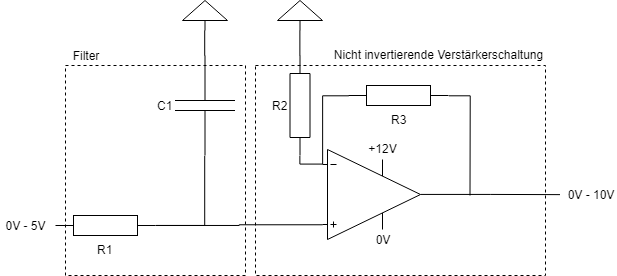
\includegraphics[scale=0.555]{Schema_Verstaerkerschaltung.png}	
		\caption{Schema Verstärkerschaltung}\label{fig:Verstaerkerschaltung}
	\end{minipage}	
	% 
	\begin{minipage}[b]{.23\textwidth}
		\centering
		\begin{tabular}{|l|l|}
			\hline
			R$_1$ & \SI{16}{k\Omega} 	\\ 	\hline
			R$_2$ & \SI{12}{k\Omega} 	\\ 	\hline
			R$_3$ & \SI{12}{k\Omega} 	\\	\hline
			C$_1$ & \SI{10}{\mu F} 		\\	\hline
		\end{tabular}
		\caption{Werte der Bauteile}
		\label{tab:Verstaerkerschaltung}
	\end{minipage}
\end{figure} 



Nach dem Aufbau der Verstärkerschaltung wurde die Ausgangsspannung bei einem duty-cycle von 1 gemessen. Dabei wurde ein Wert von \SI{9.885}{V} gemessen. Dies bedeutet das der Thyristorsteller nicht voll ausgesteuert werden kann. Deshalb wurde bei der Verstärkerschaltung die Verstärkung erhöht. 

\begin{equation}
\frac{12k\Omega}{11k\Omega} = 1.09
\end{equation}
Dies resultiert in eine Verstärkung von:
\begin{equation}
V_u = 1 + \frac{12k\Omega}{11k\Omega} = 2.09
\end{equation}
Nach dem Einbau des neuen Widerstandes wurde eine Spannung von \SI{10.2}{V} am Ausgang gemessen. Somit kann der Thyristorsteller voll ausgesteuert werden.

\subsection{Laboraufbau mit einem Widerstand}
Nach dem Feststellen der Funktionalität der Spannnungsverstärkungsschaltung konnte mit dem Laboraufbau begonnen werden. Hierzu wurde ein variabler Culatti-Widerstand als Last benutzt. Dieser hat den Vorteil das die Last bei allen Phasen symetrisch ist. Um den Strom klein zu halten, wurde ein Widerstand von \SI{150}{\Omega} gewählt. Der Aufbau der Messschaltung ist auf der Abbildung \ref{fig:Messaufbau} ersichtlich. 

\begin{figure}[ht!]
	\centering
	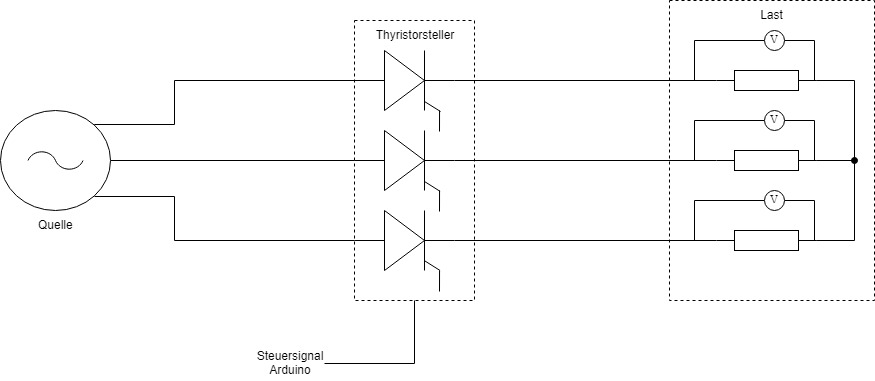
\includegraphics[width=\textwidth]{Messaufbau.png}	
	\caption{Schema Messaufbau}\label{fig:Messaufbau}
\end{figure}

Um zu analysieren wie sich die Spannung bei der Last in Dreieck verläuft, wurde die Last auch in Dreieck geschaltet werden.

\subsection{Laboraufbau mit einer ASM}
Gleich wie beim Laboraufbau wurde bei diesen Versuchen eine ASM als Motor in den Stromkreis geschaltet. Dabei wurde auch wieder der Motor in Stern und in Dreieck geschaltet. Für die ASM wurde eine kleine Maschine der Marke Lukas Nülle mit einer Leistung von \SI{0.3}{kW} verwendet. Dies hat den Grund, dass bei dieser Maschine ein Drehzahlgeber vorhanden war um die Drehzahlen messen zu können. Da die Maschine nicht wie der Widerstand, eine rein Ohmsche Last ist, verhielten sich die Spannungen anders. Ein weiterer interessanter Punkt bei dem Motor ist, dass wenn die Spannung abgeschaltet wird, die Motor sich noch eusdrehen muss und so sehr träge auf Veränderungen reagiert.

\subsection{Arduino}
Das Arduino-Programm, welches den Thyristorsteller ansteuert, wurde mit der Arduinosoftware geschrieben. Vorteil des Arduinos ist, dass die Software Open-source ist und sich für fast jede erdenkliche Arbeit auf dem Internet Beispielcodes befinden. Desweitern ist eine grosse Versibilität durch den Arduino gewährleistet. Mit den verschiedenen I/O Pins können Spannungen bis zu \SI{5}{V} gemessen und DC-Spannungen mit einem PWM ausgegeben werden.

\subsubsection{Phasenanschnittssteuerung mit Arduino}
Die Phasenanschnittssteuerung wird der einfachen \SI{0}{V} bis \SI{10}{V} Ansteuerung des Thyristorstellers gemacht. Dabei ist die Ansteuerungskennlinie linear und so ensprechen \SI{5}{V} einem Zündwinkel von 90\textdegree. Diese Ansteuerungsbereich muss nur auf die 0 bis 255 Werte umgerechnet werden, da der analogWrite Bereich des Arduinos so konzipiert ist. Wenn so z.B. ein Winkel von 90\textdegree \hspace{0.02cm} erwünscht ist, muss ein Wert von 127 ausgegeben werden.

\subsubsection{Schwingungspaketsteuerung mit Arduino}
Die Schwingungspaketsteuerung funktioniert mit dem Thyristorsteller nicht so einfach, da dieser für Phasenanschnitt gedacht ist. Jedoch kann beim Arduino umgeschaltet werden zwischen HIGH und LOW mit einer bestimmten Zeitverzögerung dazwischen. Das Problem was sich dabei stellt, ist dass der Thyristorsteller und die Spannungsverstärkerschaltung beide zusammen eine Zeitverzögerung von \SI{0.2}{s} haben. So schaltet der Sinus verzögern ein und dies resultiert in einem Hochfahren von \SI{0.35}{s}. So verhält sich die Schwingungspaketsteuerung mehr wie ein Auf- und Absteuern.

\subsubsection{Auf- und Absteuern}
Um das Auf- und Absteuern zu implementieren wurde die beiden vorherigen Verfahren kombiniert. Anstatt jedoch nur einen Winkel vorzugeben, wurde mit einer for-Schleife die Ansteuerungsspannung und so der Zündwinkel linear erhöht. Sobald sich die Spannung auf dem Maximum befindet, wird für \SI{0.2}{s} gewartet. So wird für eine kurze Zeit die maximale Spannung ausgegebn. Danach wird mit einer zweiten for-Schleife runtergefahren. Die Geschwindigkeit des Hoch- \& Runterfahrens kann verändert werden. Die Auswirkungen der Geschwindigkeit der Steigung wird im Kapitel \todo{Kapitel mit Steigung} genauer erklärt. Wenn die minimale Spannung erreicht ist, wird \SI{0.1}{s} gewartet bis das nächste Hochfahren anfängt, dies hat den Grund da sonst das Spannungssignal nicht auf Null geht. Diese zwei for-Schleifen befindet sich in einer driten for-Schleife. Diese ist dafür zuständig, mittels Schwingungspakertsteuerung einstellen zu können wieviele Hoch- \& Runterfahren gemacht werden bevor der ganze Zyklus wieder von vorne beginnt. Wenn z.B. fünf Schwingungspakete von zehn durchgeschaltet werden, bedeutet dies, dass fünfmal Hoch- \& Runtergefahren wird und danach werden die nächsten fünf Schwingungspakete gesperrt.

\subsubsection{Auf- und Absteuern lanngsam}
Für das langsamen Auf- und Absteuern wird wie der Name schon sagt, langsamer als bei dem normalen Sanft Anlasser hochgefahren. Zusätzlich wird nach dem erreichen der maximalen Spannung eine Verzöerung von \SI{6}{s} eingebaut, bis das Programm wieder Runterfährt. Desweitern bleibt man nach dem erreichen der minimalen Spannung für \SI{3}{s} auf 0. Danach fährt das Programm wieder hoch. Dies enspricht auch einem Auf- und Absteuern aber wie im Kapitel \todo{Kapitel mit Steigung} erklärt, verhaltet sich das FFT in diesem Fall ganz anders als mit dem normalen Auf- und Absteuern.

\subsubsection{Drehzahlmessung für eine Reglerauslegung}
Um die Drehzahl der ASM messen und regeln zu können, wurde eine Drehzahlregelung eingebaut. Dabei wird die Spannung über dem Drehzahlgeber gemessen. Die Spannung beträgt bei einer von Drehzahl von \SI{2800}{U/min} \SI{58.8}{V}. Die Spannung ist linear von der Drehzahl abhängig, und beträgt so bei z.B. \SI{1400}{U/min} \SI{29.4}{V}. Da diese Spannung zu hoch ist um mit dem Arduino messen zu können, wurde ein Spannungsteiler eingebaut. 

\begin{equation}
4.94 V = 58.8 V \cdot \frac{56k\Omega}{56k\Omega + 611k\Omega}
\end{equation}

Somit kann die Spannung mit dem Arduino gemessen werden. Dabei wird die Spannung mit 1024 verschiedenen Stufen gemessen. So enspricht der Wert 512 einer Spannung von \SI{2.5}{V}.
\todo{Einfügen Quelle für Spannungsmessung} So kann mit dieser Spannung weiter gearbeitet werden. Zusätzlich wird dieser Wert mit den Widerstandswerten des Spannungsteiler auf die Orginalspannung zurück gerechnet. Für den Regler wird für den Sollwert ein Spannungswert vorgegeben. Damit kann von dem Sollwert der Istwert abgezogen werden, um die Differenz zu erhalten. Da der Ausgabewert einem Wert zwischen 0 und 255 entspricht, muss die Differenz umgerechnet werden. Zusätzlich zur Differenz, wird ein PI-Regler benötigt. 
Mit der Formel: \cite{Quelle_Marco} 
\begin{equation}
Y(k) = Y(k-1)+ B_0U(k)+B_1U(k-1)
\end{equation}
Wobei $Y$ der Ausgangsspannung, $U$ der Differenzspannung und $k$ dem Laufparameter ensprechen \cite{PI_Regler}. Die Parameter $B_0$ und $B_1$ werden folgendermassen berechnet:
\begin{equation}\label{eq:B0}
B_0 = \left(K_p + \frac{K_iT}{2}\right) 
\end{equation}
\begin{equation}\label{eq:B1}
B_1 = -\left(K_p - \frac{K_iT}{2}\right) 
\end{equation}

Nachdem dies berechnet ist, muss die Spannungsdifferenz von der Ausgangsspannung subtrahiert werden. Das Resultat muss danach in die 0 bis 255 Werte umgerechnet werden. Die Werte der Ausgangsspannung und der Differenzspannung werden nach der Ausgabe in den Laufparameter $k-1$ geladen. Das Problem mit dem PI-Regler ist, dass der Thyristorsteller und die Spannungsverstärkung eine Totzeit besitzen. Dadurch ist das Auslegen eines guten Reglers nicht möglich. Durch das Gespräch mit anderen Studenten, wurde festgestellt das ein Smithprädiktor \cite{Regelungstechnik_Buch} Abhilfe verschaffen könnte. Dieser rechnet die Totzeiten in das System und dieses kann so genauer geregelt werden. Jedoch wurde der Smithprädikator nicht mehr implementiert. Der Code für die Drehzahlregelung befindet sich im Anhang. \todo{Kapitel angeben}

\begin{figure}[ht!]
	\centering
	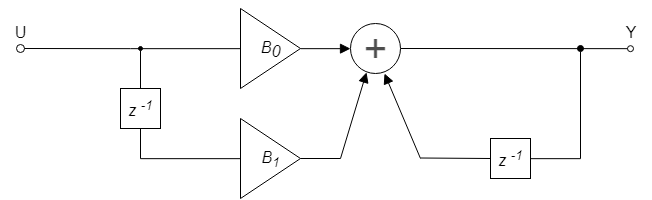
\includegraphics[width=\textwidth]{BlockdiagrammPI.png}	
	\caption{Blockdiagramm eines digitalen PI-Reglers}\label{fig:PIRegler}\cite{PI_Regler}
\end{figure}








\section{Normen}


\section{Resultate des Messaufbaus}
In diesem Kapitel werden die Messresultate des Laboraufbaus analysiert und mit den Werten der Simulationen und den Normen verglichen. Hierbei wurden die Daten der Messungen als .csv Datei gespeichert und anschliessend mit Matlab dargestellt. Ausserdem ist es möglich die FFTs der Signale zu berechnen.\\
Es sind nur die Messungen des Widerstandes und der ASM, die in Stern geschaltet sind aufgelistet. Die Messungen in Dreieck sind hier nicht aufgeführt, sie  befinden sich als Matlabdateien digital auf dem USB-Stick. \todo{angeben ob als USB Stick/CD oder sonst abgegeben}


\newpage
\subsection{Messungen Ströme}
Die Ströme der verschiedenen Ansteuerungarten und Verbrauchern sind auf zu- und unzulässige Oberschwingungen zu untersuchen. Sie müssen zwingend die Werte der Normen \ref{sec:Normen} einhalten. Ist dies der Fall, werden anschliessend noch die Spannungen untersucht. Halten Ansteuerungsarten die Normen nicht ein werden die Spannungen nicht behandelt. Bei den Schwingungspaketsteuerungen werden die Ströme nicht angeschaut, da die nicht von Interesse sind. Damit man jedoch einen Vergleich zur Simulation hat, ist diese Ansteuerung bei der Spannung aufgelistet. Die Vergleiche werden immer mit Hilfe der FFT-Funktion von Matlab durchgeführt. 

\subsubsection{Messungen Widerstand}

Die Resultate der Strommessungen sind wie folgt aufgebaut. Bei den Abbildungen \ref{fig:Mess_Widerstand_Phas_60grad_stroeme}, \ref{fig:Mess_Widerstand_Phas_90grad_stroeme}, \ref{fig:Mess_Widerstand_Sanft_stroeme} und \ref{fig:Mess_Widerstand_Sanft_langsam_stroeme} sind zuerst die Ströme, die durch den Culatti fliessen dargestellt. Der Culatti ist ein ohmscher Widerstand mit dem Wert von \SI{150}{\Omega} pro Strang. Der maximale Effektivstrom, der dabei durchgelassen werden darf ist \SI{2.4}{A}. Die zweite Grafik zeigt das FFT des gemessenen Stromes, jedoch nur von einer Phase, an. Da sich alle drei Phasen, gleich verhalten, werden die anderen zwei nicht angezeigt. Da die Grenzwerte der Oberschwingungsströme einen maximalen Wert von bis zu \SI{16}{A} Effektivwert behandelt, wurde der gemessene Wert auf die \SI{16}{A} hochgerechnet. Dies ist in der dritten Grafik der jeweiligen Abbildung ersichtlich. Anschliessend berechnete man von diesen Ströme das FFT und verglich die Werte der Amplitude tabellarisch mit den dazugehörigen Normen \ref{sec:Stromnormen}, ersichtlich in der Tabelle \ref{tab:Grenzwerte_Normen}.

\subsubsection*{Phasenanschnitt 60\textdegree}

In der Abbildung \ref{fig:Mess_Widerstand_Phas_60grad_stroeme} ist das Stromsignal mit einem Phasenanschnittswinkel von 60\textdegree \hspace{0.02cm} ersichtlich. 

\begin{figure}[ht!]
	\centering
	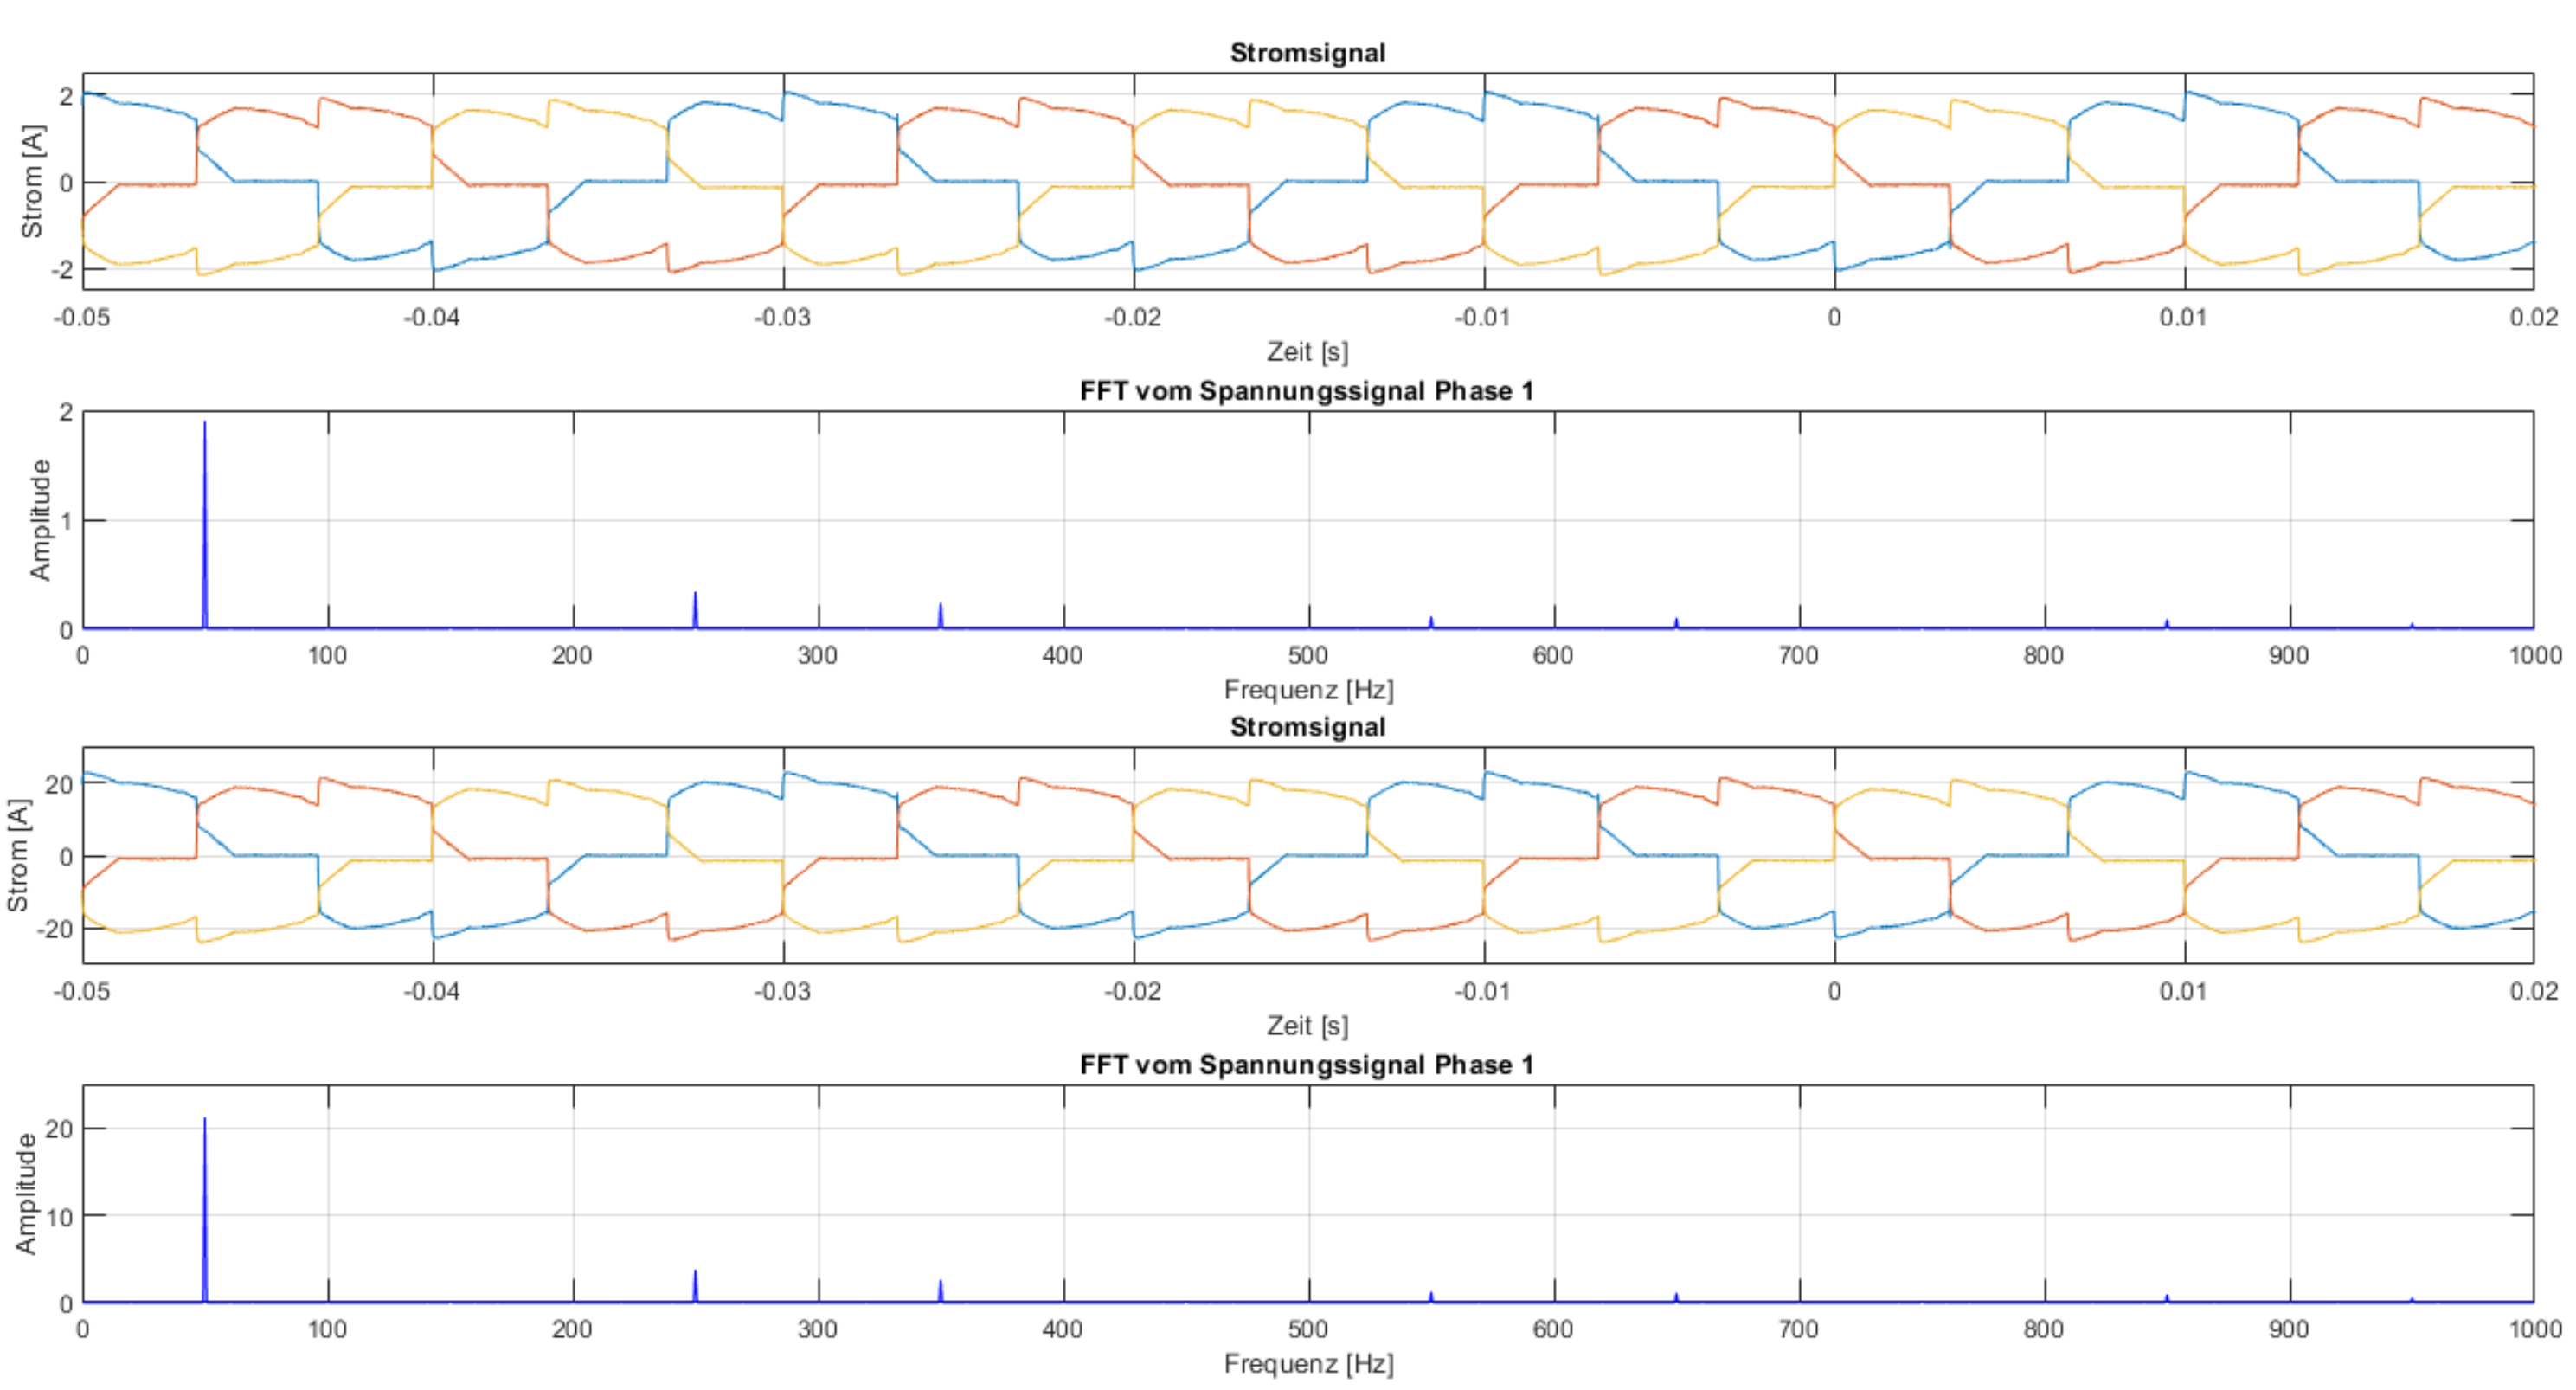
\includegraphics[width=\textwidth]{Messung_Widerstand_Phas_60grad_stroeme.png}	
	\caption{Messung mit Phasenanschnitt 60\textdegree}\label{fig:Mess_Widerstand_Phas_60grad_stroeme}
\end{figure}


\begin{table}[ht!]
	\centering
	\begin{tabular}{|l|l|l|}
		\hline
		Oberschwingungsordnung & Amplitude [A] 	& Verhältnis zur Grundschwingung	\\ \hline
		1                      & 21.1996   		& 100\%								\\ \hline
		5                      & 3.7851    		& 17.86\%							\\ \hline
		7                      & 2.6127    		& 12.32\%							\\ \hline
		11                     & 1.2267    		& 5.79\%							\\ \hline
	\end{tabular}
	\caption{Amplitudenwerte bei den harmonischen Oberschwingungen bei Phasenanschnitt 60\textdegree}\label{tab:Phas_60_Stroeme}
\end{table}
%Die Höhe der Amplituden der Oberschwingungen der Tabelle \ref{tab:Phas_60_Stroeme} können mit den Normen in der Tabelle \ref{tab:Grenzwerte_Normen} verglichen werden. Dabei wird festgestellt, dass die Werte der Messung höher sind als die Normen zulassen.

Wenn die Werte der Messungen in der Tabelle \ref{tab:Phas_60_Stroeme} mit der Werte der Normen in der Tabelle \ref{tab:Grenzwerte_Normen} verglichen werden, ist ersichtlich, dass die Amplitudenwerte bei der 5. bis 11. Oberschwingungsordnung zu hoch sind. Es kann gesagt werden, dass sich der Phasenanschnitt mit 60\textdegree \hspace{0.02cm} nicht eignet um den Widerstand anzusteuern, da dies nicht den Normen entspricht. Die Spannungen werden deshalb nicht mehr untersucht. 


\subsubsection*{Phasenanschnitt 90\textdegree}

Die Abbildung \ref{fig:Mess_Widerstand_Phas_90grad_stroeme} zeigt die Ansteuerung mit einem Phasenanschnitt von 90\textdegree \hspace{0.02cm}. 

\begin{figure}[ht!]
	\centering
	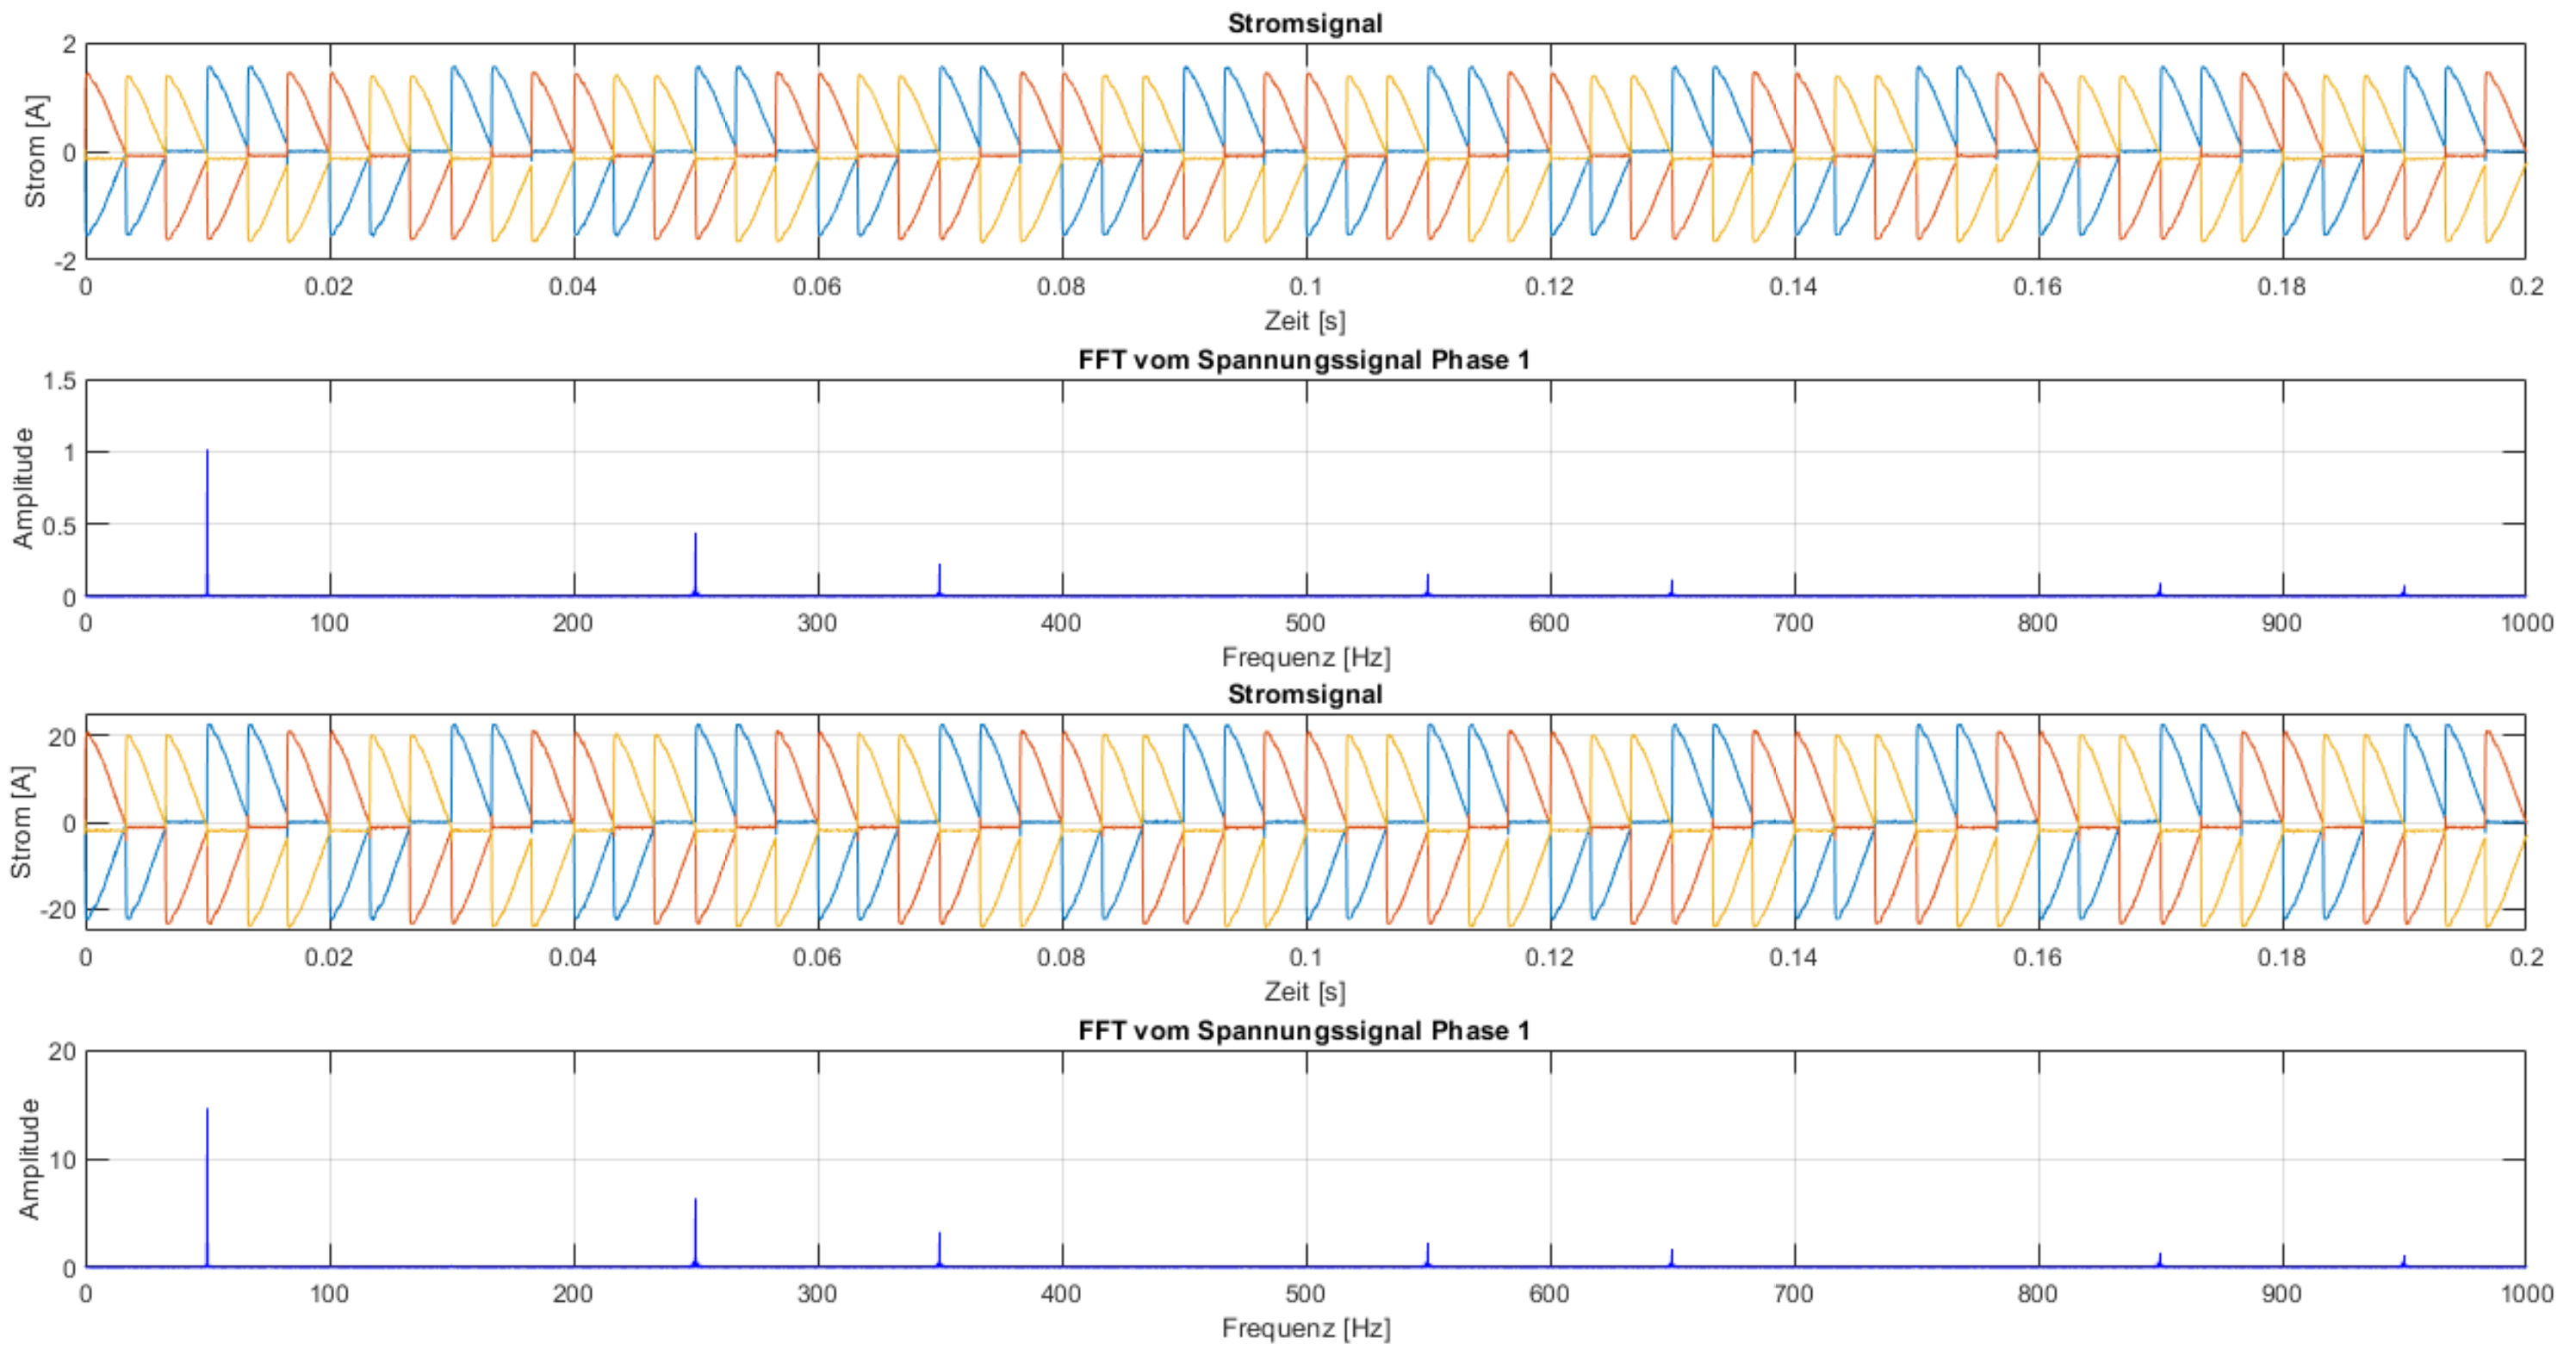
\includegraphics[width=\textwidth]{Messung_Widerstand_Phas_90grad_stroeme.png}	
	\caption{Phasenanschnitt 90\textdegree}\label{fig:Mess_Widerstand_Phas_90grad_stroeme}
\end{figure}

\begin{table}[ht!]
	\centering
	\begin{tabular}{|l|l|l|}
		\hline
		Oberschwingungsordnung 	& Amplitude [A] & Verhältnis zur Grundschwingung	\\ \hline
		1       				& 14.647   		& 100\%								\\ \hline
		5      					& 6.3481    	& 43.34\%							\\ \hline
		7      					& 3.2571    	& 22.24\%							\\ \hline
		11      				& 2.273    		& 15.52\%							\\ \hline
	\end{tabular}
	\caption{Amplitudenwerte bei den harmonischen Oberschwingungen bei Phasenanschnitt 90\textdegree}\label{tab:Phas_90_Stroeme}
\end{table}

Die Amplitudenwerte der 5 bis 11 Oberschwingungsanordnung, erkennbar in der Tabelle \ref{tab:Phas_90_Stroeme}, sind auch bei dieser Ansteuerung, im Vergleich zu den Normen \ref{tab:Grenzwerte_Normen}, zu hoch. Somit eignet sich auch der Phasenanschnitt mit 90\textdegree \hspace{0.02cm} nicht, den Widerstand anzusteuern. Auf die Spannung wird ebenfalls hier nicht mehr eingegangen. 


\newpage
\subsubsection*{Hartes Auf- und Absteuern}

In der Abbildung \ref{fig:Mess_Widerstand_Sanft_stroeme} ist das harte Auf- und Absteuern des Widerstands erkennbar. 

\begin{figure}[ht!]
	\centering
	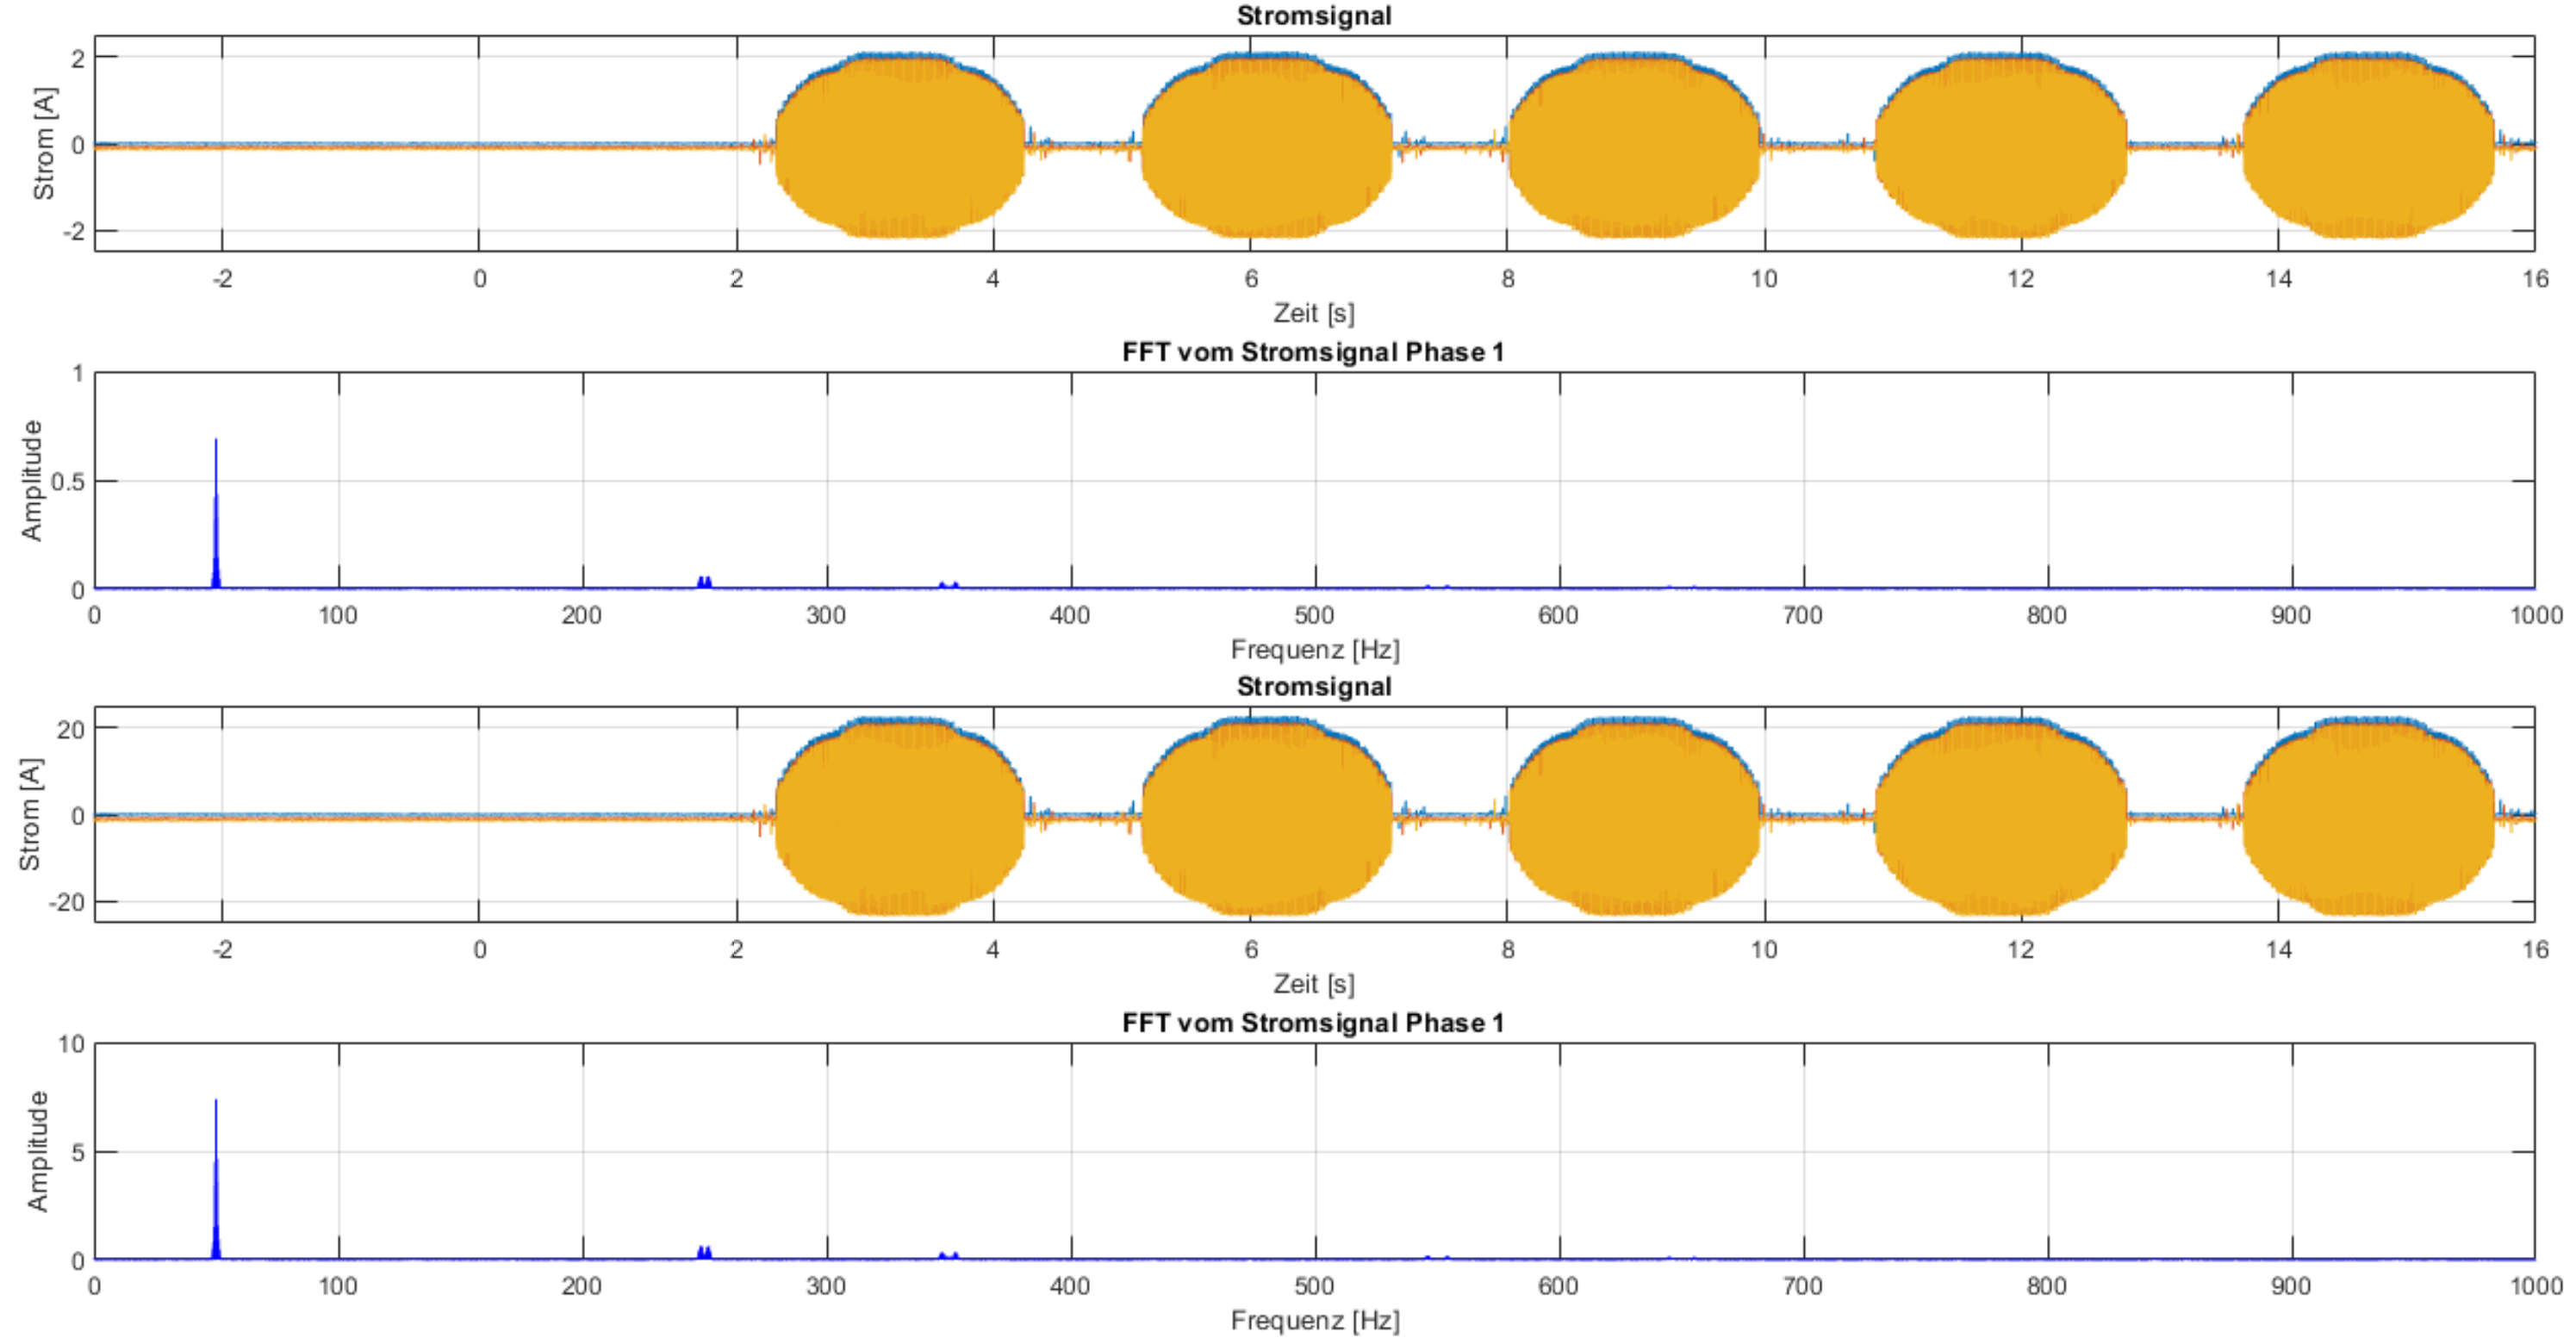
\includegraphics[width=\textwidth]{Messung_Widerstand_Sanft_stroeme.png}	
	\caption{Messung mit dem harten Auf- und Absteuern}\label{fig:Mess_Widerstand_Sanft_stroeme}
\end{figure}


\begin{table}[ht!]
	\centering
	\begin{tabular}{|l|l|l|}
		\hline
		Frequenz {[}Hz{]} & Amplitude {[}A{]} & Verhältnis zur Grundschwingung	\\ \hline
		49.3              & 1.5146            & 20.51\%							\\ \hline
		49.6              & 4.4853            & 60.73\%							\\ \hline
		49.7              & 2.618             & 35.45\%							\\ \hline
		50                & 7.3857            & 100\%							\\ \hline
		50.05             & 3.73              & 50.5\%							\\ \hline
		50.35             & 4.662             & 63.12\%							\\ \hline
		50.7              & 1.5504            & 21\%							\\ \hline
		248.65            & 0.6226            & 8.43\%							\\ \hline
		250               & 0.0883            & 1.2\%							\\ \hline
		251.45            & 0.6               & 8.12\%							\\ \hline
	\end{tabular}
	\caption{Amplitudenwerte bei verschiedenen Frequenzen beim hartem Auf- und Absteuern}\label{tab:Sanft_stroeme}
\end{table}
Da beim harten Auf- und Absteuern bereits die 5. harmonische Oberschwingung, eine Amplitudenwert von  \SI{0.1}{A} hat, wurde darauf verzichtet, weitere Werte der harmonischen Schwingungen tabellarisch aufzulisten. Jedoch sind bei dieser Messung die Sub- und Zwischenharmonische sehr interessant. Diese sind in der Tabelle \ref{tab:Sanft_stroeme} aufgeführt. Es ist ersichtlich, dass die Werte der Sub- und Zwischenharmonischen um \SI{50}{Hz}, mehr als die Hälfte der Grundschwingung entsprechen. Diese sogenannten Seitenbänder sind auch bei den weiteren harmonischen Oberwellen erkennbar. Sie sind jedoch kleiner als die, um die \SI{50}{Hz}. Vergleicht man die Werte der Amplitude der Harmonischen sind sie im Bereich der erlaubten Grenzwerte. Deshalb wird noch eine Untersuchung der Spannung vorgenommen.


\newpage
\subsubsection*{Sanftes Auf- und Absteuern}\label{sec:Sanft_Widerstand_stroeme}
In Abbildung \ref{fig:Mess_Widerstand_Sanft_langsam_stroeme} erkennt man ein sanftes Auf- und Absteuern der Ströme.

\begin{figure}[ht!]
	\centering
	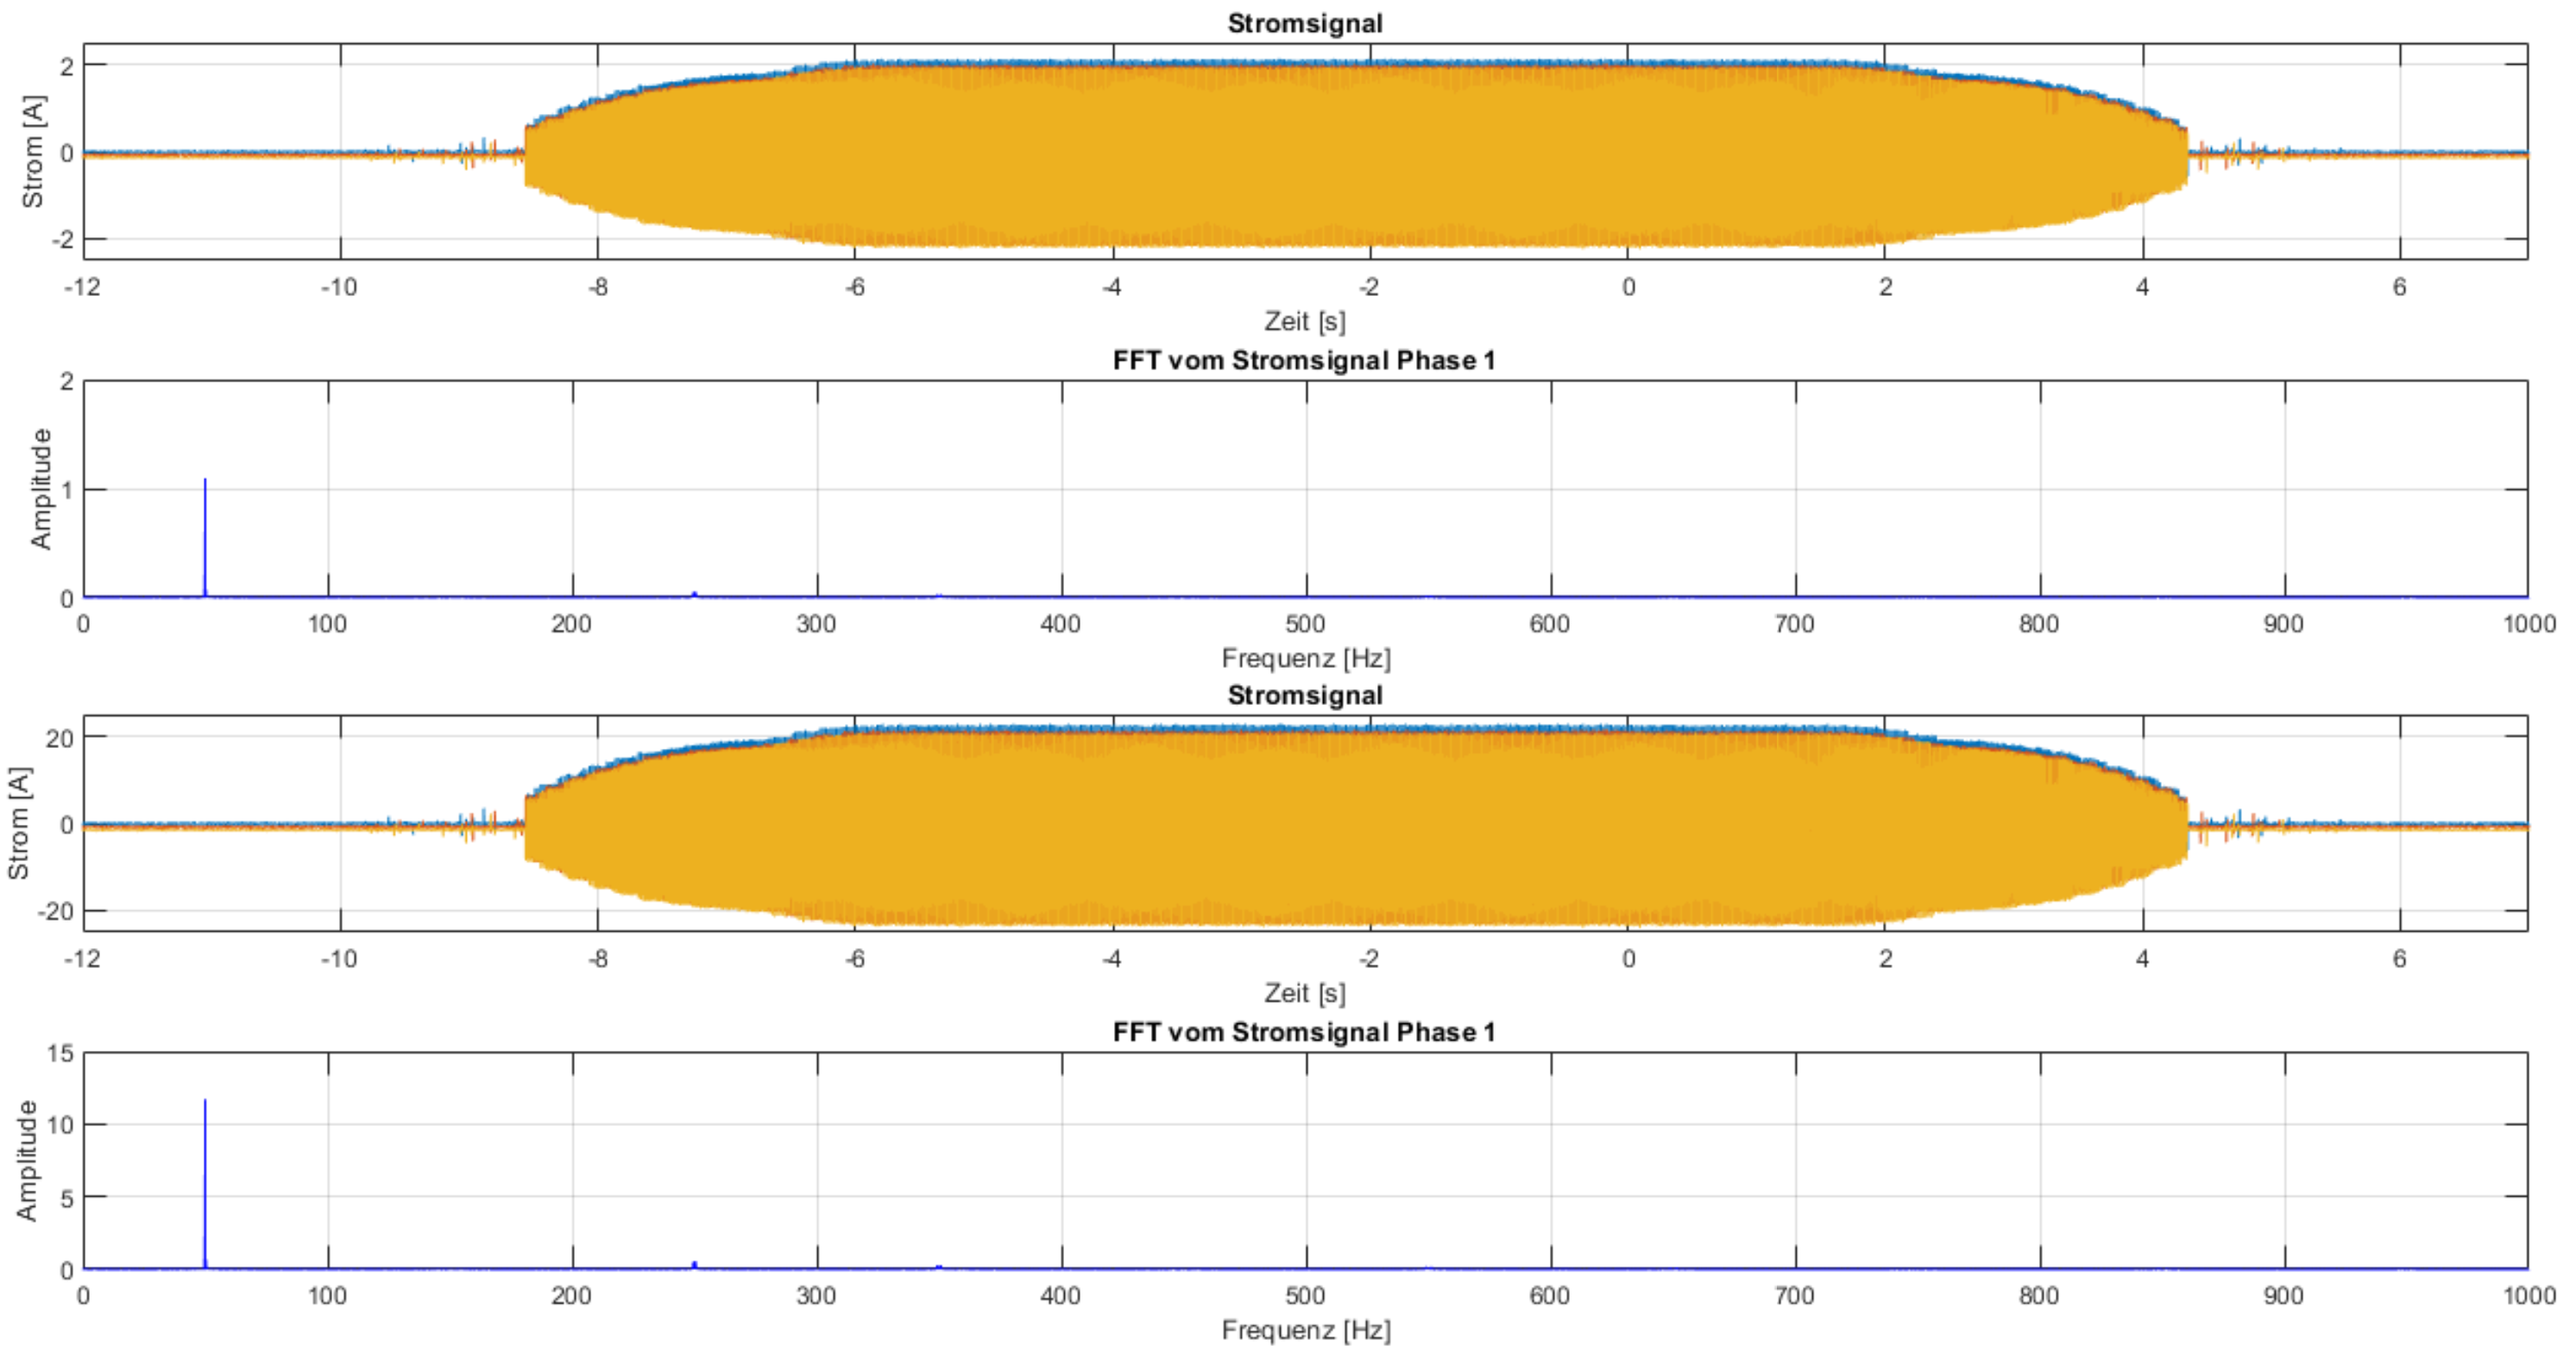
\includegraphics[width=\textwidth]{Messung_Widerstand_Sanft_langsam_stroeme.png}	
	\caption{Messung mit sanftem Auf- und Absteuern}\label{fig:Mess_Widerstand_Sanft_langsam_stroeme}
\end{figure}

\begin{table}[ht!]
	\centering
	\begin{tabular}{|l|l|l|}
		\hline
		Frequenz {[}Hz{]} & Amplitude {[}A{]} & Verhältnis zur Grundschwingung	\\ \hline
		49.8              & 1.148             & 9.8\%							\\ \hline
		49.85             & 1.786             & 15.25\%							\\ \hline
		49.9              & 1.519             & 12.97\%							\\ \hline
		49.95             & 6.703             & 57.22\%							\\ \hline
		50                & 11.715            & 100\%							\\ \hline
		50.05             & 7.136             & 60.91\%							\\ \hline
		50.1              & 1.473             & 12.57\%							\\ \hline
		50.15             & 1.923             & 16.41\%							\\ \hline
		249.65            & 0.563             & 4.81\%							\\ \hline
		250               & 0.186             & 1.59\%							\\ \hline
		250.35            & 0.559             & 4.77\%							\\ \hline
	\end{tabular}
	\caption{Amplitudenwerte bei den harmonischen Oberschwingungen beim sanftem Auf- und Absteuern}\label{tab:Sanft_langsam_stroeme}
\end{table}
Es ist zu erkennen, dass auch hier fast keine harmonische Oberwellen vorhanden sind. Die Amplitude der Grundschwingung ist jedoch höher als beim harten Auf- und Absteuern. Dies hat den Grund, dass länger auf der vollen Leistung gefahren wurde. Beim sanften Auf- und Absteuern ist das Hoch- und Runtergefahren langsamer, deshalb ist das Seitenband bei \SI{50}{Hz} kleiner. Dies erkennt man auch schon beim visuelle Vergleich der beiden Abbildungen \ref{fig:Mess_Widerstand_Sanft_langsam_stroeme} und \ref{fig:Mess_Widerstand_Sanft_stroeme}. Im Vergleich zum harten Auf- und Absteuern, ist die 5. Harmonische 0.39\% grösser, welches einem sehr kleinen Unterschied entspricht. Jedoch sind die Peaks der Seitenbänder näher bei \SI{50}{Hz}. Die Peaks des Seitenbandes bei \SI{250}{Hz} sind bei dem sanften Auf- und Absteuern kleiner als die beim harten Auf- und Absteuern.



\newpage
\subsubsection{Messungen Asynchronmaschine}
Um zu analysieren, wie sich das Signal bei einer ohmsch-induktiver Last verhält, wurden die Messungen mit einem Asynchronmotor wiederholt. Die Strommessungen der ASM wurde mit den bekannten Phasenanschnittswinkeln und mit dem sanften Auf- und Absteuern vorgenommen. Dies hat den Grund, dass keine Anwendungen für das harte Auf- und Absteuern oder der Schwingungspaketsteuerung vorhanden sind. Ausserdem wird in der Praxis meistens der Phasenanschnitt verwendet. Wie auch schon beim Widerstand muss der Strom bei der ASM auf die \SI{16}{A} hochgerechnet werden, um diese mit den Norm tabellarisch vergleichen zu können. Die Messungen der Asynchronmaschine sind ähnlich aufgebaut wie die des Widerstands. Einzig das Spannungssignal des Drehzahlgebers wurde hinzugefügt. Es ist erkennbar, dass das jeweilige Hochfahren des Stromes einen Einfluss auf das Spannungssignal des Drehgeber hat. Je harter man Hochfährt desto steiler wird die Kurve des Spannungssignal des Drehgeber. 


\subsubsection*{Phasenaschnitt 60\textdegree}
In Abbildung \ref{fig:Mess_Phas_60grad_stroeme} erkennt man ein einen Phasenanschnitt von 60\textdegree der Ströme.

\begin{figure}[ht!]
	\centering
	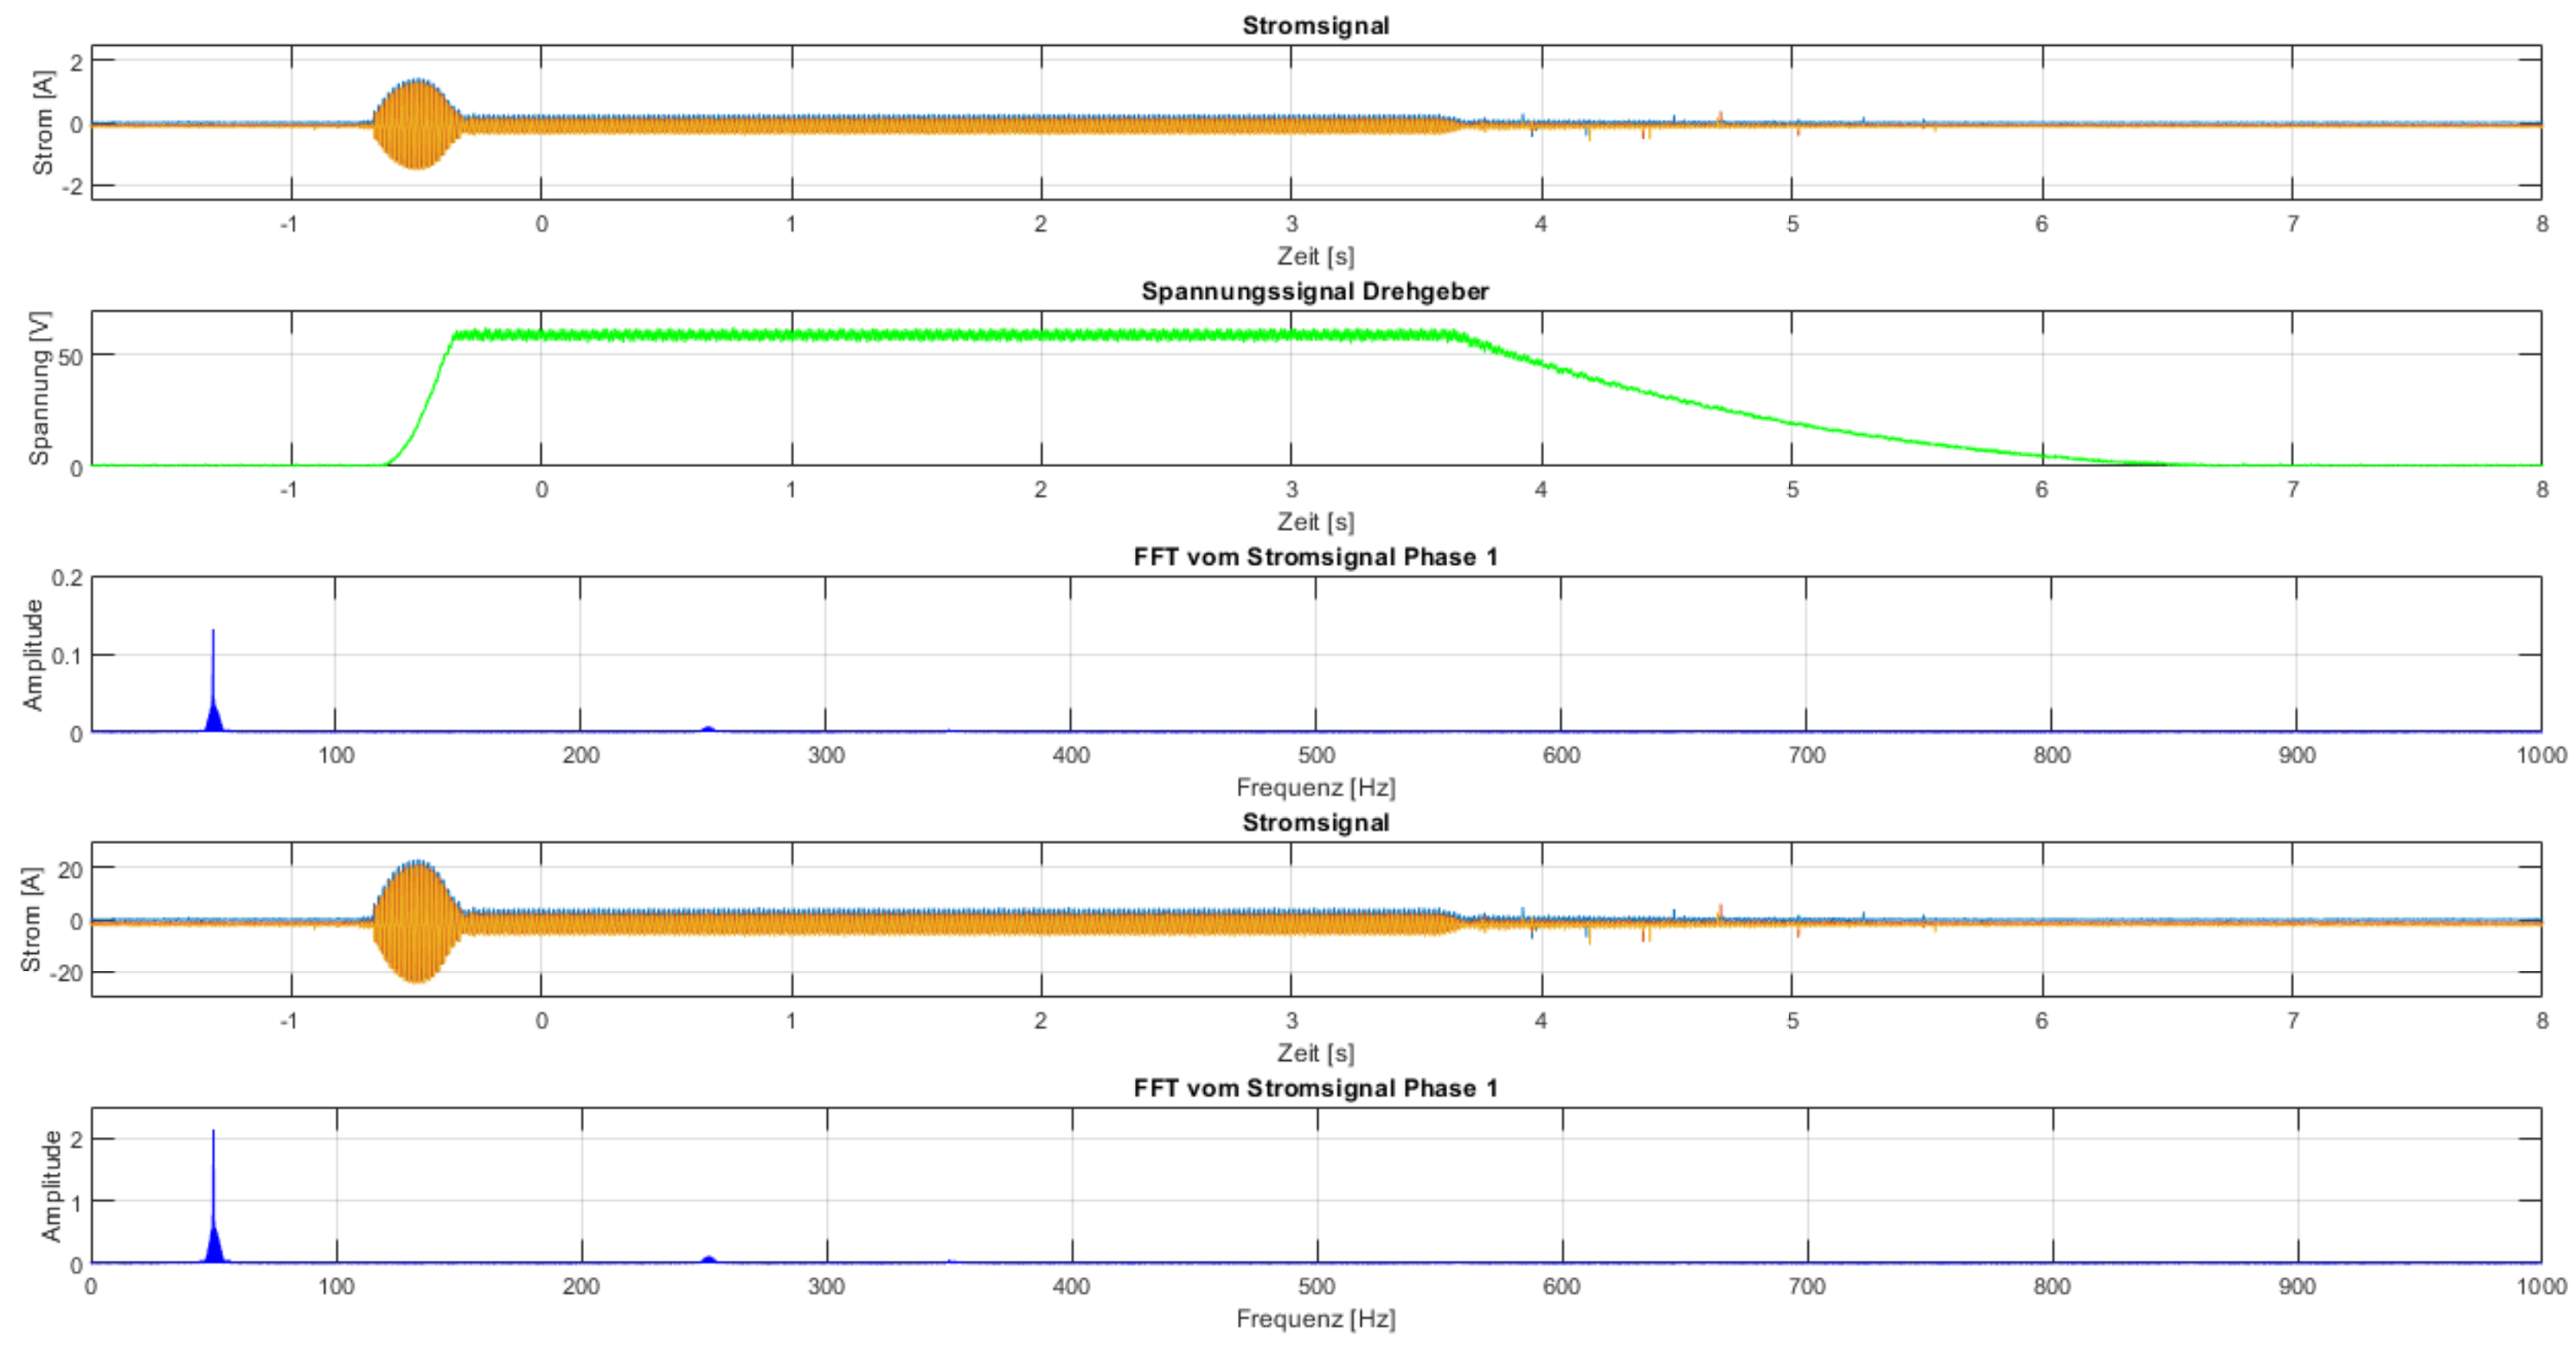
\includegraphics[width=\textwidth]{Messung_ASM_Phas_60grad_stroeme.png}	
	\caption{Messung mit Phasenanschnitt 60\textdegree}\label{fig:Mess_Phas_60grad_stroeme}
\end{figure}

\begin{table}[ht!]
	\centering
	\begin{tabular}{|l|l|l|}
		\hline
		Frequenz {[}Hz{]} & Amplitude {[}A{]} & Verhältnis zur Grundschwingung	\\ \hline
		49.7              & 0.76              & 35.53\%							\\ \hline
		49.9              & 1.317             & 61.57\%							\\ \hline
		50                & 2.139             & 100\%							\\ \hline
		50.1              & 1.53              & 71.53\%							\\ \hline
		50.3              & 0.675             & 31.56\%							\\ \hline
		250               & 0.07              & 3.27\%							\\ \hline
	\end{tabular}
	\caption{Amplitudenwerte bei den harmonischen Oberschwingungen bei Phasenanschnitt 60\textdegree}\label{tab:Phas_60_ASM_stroeme}
\end{table}
Entgegen den Vorkenntnissen bei Phasenanschnitt mit einem Winkel von 60\textdegree, gibt es bei der Ansteuerung der ASM praktisch keine harmonischen Oberwellen sondern fast nur Sub- und Zwischenharmonische. Dies hat den Grund, dass ein reiner Sinus von einer Frequenz von \SI{50}{Hz} bei der maximalen Drehzahl entsteht. Die fünfte harmonische Schwingung hat eine Amplitude von \SI{0.07}{A} und hält somit die Normen \ref{sec:Stromnormen} ein. Weitere Harmonische sind nicht zu erkennen. Die Peaks des Seitenbandes um die Grundschwingung sind im Verhältnis mit bis zu 70\% sehr hoch.


\subsubsection*{Phasenaschnitt 90\textdegree}

In Abbildung \ref{fig:Mess_Phas_90grad_stroeme} erkennt man ein einen Phasenanschnitt von 90\textdegree \hspace{0.02cm} der Ströme.

\begin{figure}[ht!]
	\centering
	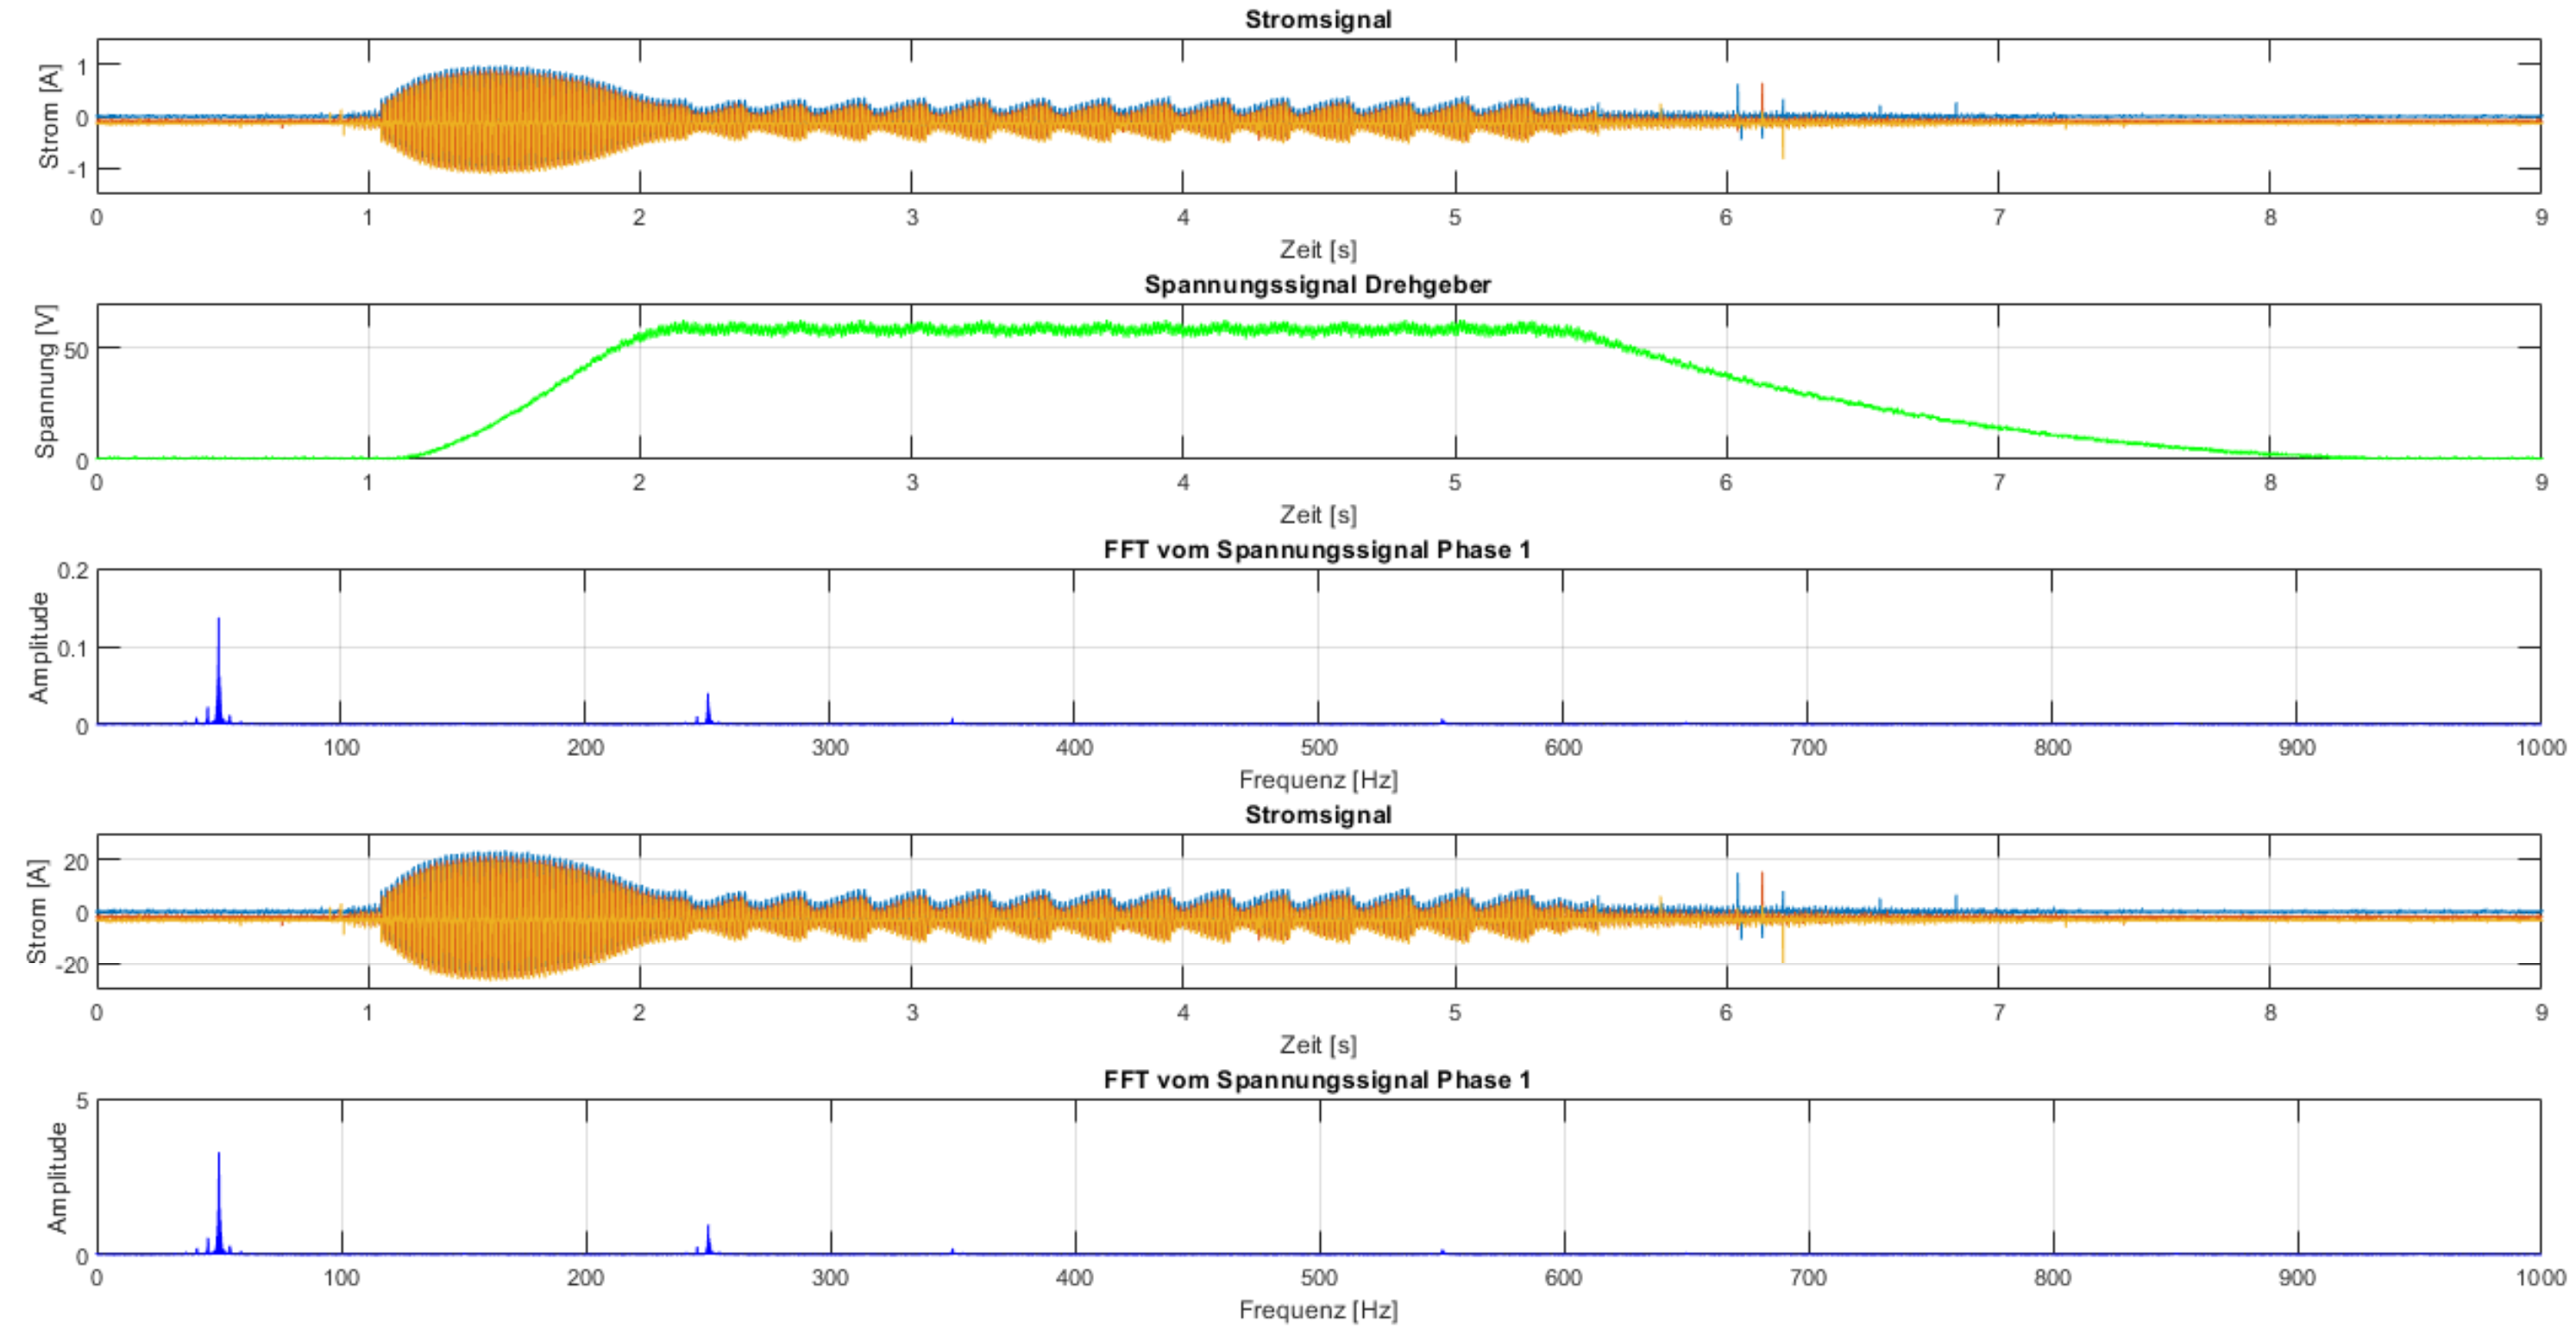
\includegraphics[width=\textwidth]{Messung_ASM_Phas_90grad_stroeme}	
	\caption{Messung mit Phasenanschnitt 90\textdegree}\label{fig:Mess_Phas_90grad_stroeme}
\end{figure}


\begin{table}[ht!]
	\centering
	\begin{tabular}{|l|l|l|}
		\hline
		Frequenz {[}Hz{]} & Amplitude {[}A{]} & Verhältnis zur Grundschwingung	\\ \hline
		49.7              & 1.399             & 42.6\%							\\ \hline
		49.9              & 2.023             & 61.61\%							\\ \hline
		50                & 3.2839            & 100\%							\\ \hline
		50.1              & 2.567             & 78.17\%							\\ \hline
		50.3              & 1.468             & 44.71\%							\\ \hline
		250               & 0.673             & 20.5\%							\\ \hline
		250.1             & 0.959             & 29.2\%							\\ \hline
		250.2             & 0.687             & 20.92\%							\\ \hline
	\end{tabular}
	\caption{Amplitudenwerte bei den harmonischen Oberschwingungen bei Phasenanschnitt 90\textdegree}\label{tab:Phas_90_ASM_stroeme}
\end{table}

Anders als bei der Ansteuerung mit dem Phasennaschnitt von 60\textdegree, treten mit 90\textdegree \hspace{0.02cm} bei der fünften Harmonischen grössere harmonische Oberwellen auf. Zusätzlich sind auch die Sub- und Zwischenharmonischen grösser als bei 60\textdegree. Auf der Abbildung \ref{fig:Mess_Phas_90grad_stroeme} ist beim Stromsignal ersichtlich, dass die Maschine schwingt. Dies wurde auch beim Testen festgestellt, dass die ASM nicht konstant auf der gleichen Drehzahl drehte. So kann diese Ansteuerungsart nicht verwendet werden um die Maschine anzusteuern. 
Im Vergleich zum Phasenanschnitt mit 60\textdegree, sind die Peaks des Seitenbandes um die Grundschwingung noch höher. Auch die fünfte Harmonische entspricht im Verhältnis zur Grundschwingung 20.5\%. Die Amplitude jedoch ist immer noch kleiner als der erlaubte Grenzwert der Norm \ref{sec:Stromnormen}. 



\subsubsection*{Sanftes Auf- und Absteuern}

In Abbildung \ref{fig:Mess_Sanft_langsam_stroeme} erkennt man ein einen sanftes Auf- und Absteuern der Ströme.

\begin{figure}[ht!]
	\centering
	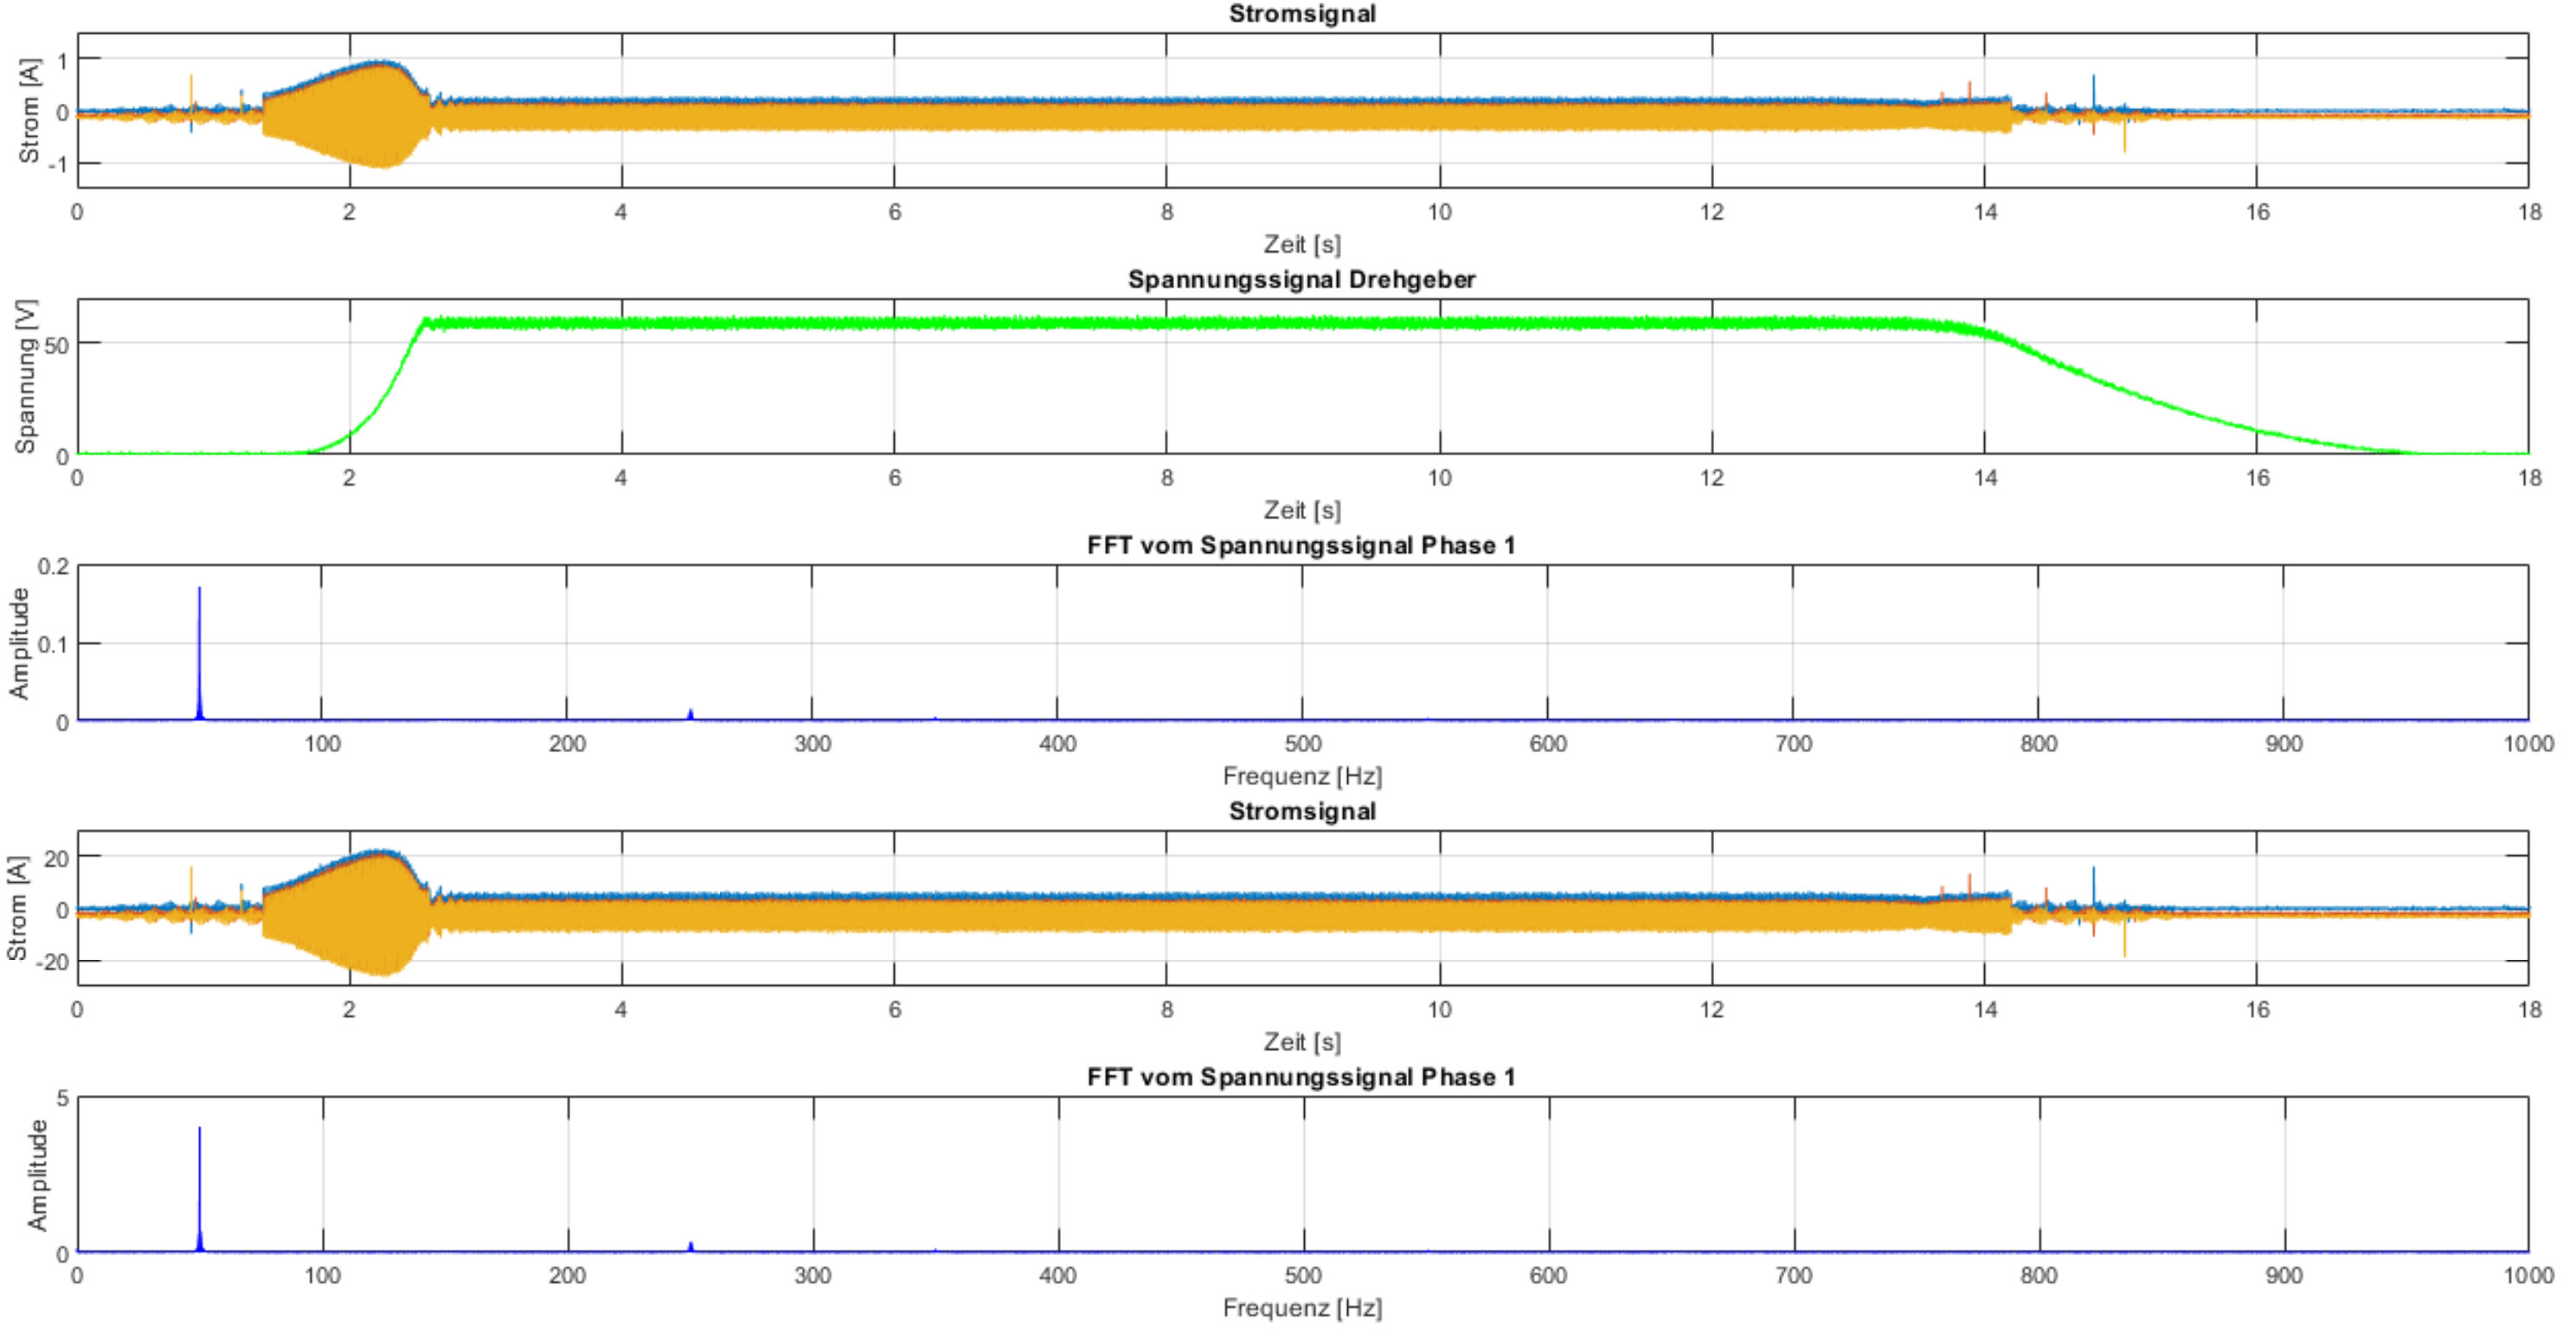
\includegraphics[width=\textwidth]{Messung_ASM_Sanft_langsam_stroeme.png}	
	\caption{Messung mit sanftem Auf- und Absteuern}\label{fig:Mess_Sanft_langsam_stroeme}
\end{figure}

\begin{table}[ht!]
	\centering
	\begin{tabular}{|l|l|l|}
		\hline
		Frequenz {[}Hz{]} & Amplitude {[}A{]} & Verhältnis zur Grundschwingung	\\ \hline
		49.8              & 0.823             & 20.51\%							\\ \hline
		49.9              & 1.064             & 26.51\%							\\ \hline
		49.95             & 1.716             & 42.76\%							\\ \hline
		50                & 4.013             & 100\%							\\ \hline
		50.05             & 1.613             & 40.19\%							\\ \hline
		50.1              & 1.141             & 28.43\%							\\ \hline
		50.2              & 0.878             & 21.88\%							\\ \hline
		250               & 0.28              & 6.98\%							\\ \hline
	\end{tabular}
	\caption{Amplitudenwerte bei den harmonischen Oberschwingungen bei sanftem Auf- und Absteuern}\label{tab:Sanft_langsam_ASM_stroeme}
\end{table}
Wie schon bei der Widerstandsmessung mit dem sanftem Auf- und Absteuern im Kapitel \ref{sec:Sanft_Widerstand_stroeme}, sind bei dieser Messung, mit der ASM, die harmonische Oberschwingungen sehr klein. Sie halten somit die Norm \ref{sec:Stromnormen} ein. In der Tabelle \ref{tab:Sanft_langsam_ASM_stroeme} sind bei verschiedenen Frequenzen die Werte der Amplituden des FFTs aufgelistet.
Die Peaks des Seitenbandes um \SI{50}{Hz} haben ein Verhältnis von bis zu 40\% zur Grundfrequenz.


\newpage
\subsection{Messungen Spannungen}

Damit man die Funktionen des Laboraufbaues mit den Simulationen vergleichen kann, wurden die Spannungen über dem Widerstand und der Asynchronmaschine mit den verschiedenen Ansteuerungsarten gemessen. Dafür wurden die Spannungssignale und das FFT als Grafik und die interessanten Werte der sub-, zwischenharmonischen und harmonischen Schwingungen tabellarisch aufgelistet. Damit auch die Spannungen mit den Normen verglichen werden können, wurde das Verhältnis der verschiedenen Oberschwingungen zur Grundschwingung in Prozent in die Tabellen eingefügt. Da die Phasenantschnittsteureungen die Normen der harmonischen Oberwellen des Stromes nicht einhalten, werden die Spannungssignale bei diesen Verfahren nicht mehr aufgezeigt. Sie sind jedoch im Anhang \ref{sec:Mess_Spannung_Widerstand} ersichtlich. Die Abbildungen in diesem Kapitel sind so aufgebaut, dass zuerst das Spannungssignal über dem Widerstand und anschliessend das daraus berechnete FFT dargestellt wurde.

\subsubsection{Messungen Widerstand}

Zuerst wird die Spannung der Schwingungspaketsteuerung mit einem Duty Cycle von 0.5 und 0.8 über dem ohmschen Widerstand untersucht. Anschliessend betrachtet man das harte und sanfte Auf- und Absteuern der Spannung über dem Widerstand. Da bei diesen Verfahren keine harmonischen Schwingungen auftreten, halten sie die Normen \ref{sec:Spannungsnormen} zu den Harmonischen ein. Die Erkenntnisse zu den Sub- und Zwischenharmonischen wird im Kapitel \ref{sec:Interpretation_Resultate} Interpretation der Resultate erläutert.

\subsubsection*{Schwingungspaket mit Duty Cycle von 0.5}

In Abbildung \ref{fig:Mess_Schwing_50} ist die Schwingungspaketsteuerung mit einem Duty Cycle von 0.5 dargestellt.


\begin{figure}[ht!]
	\centering
	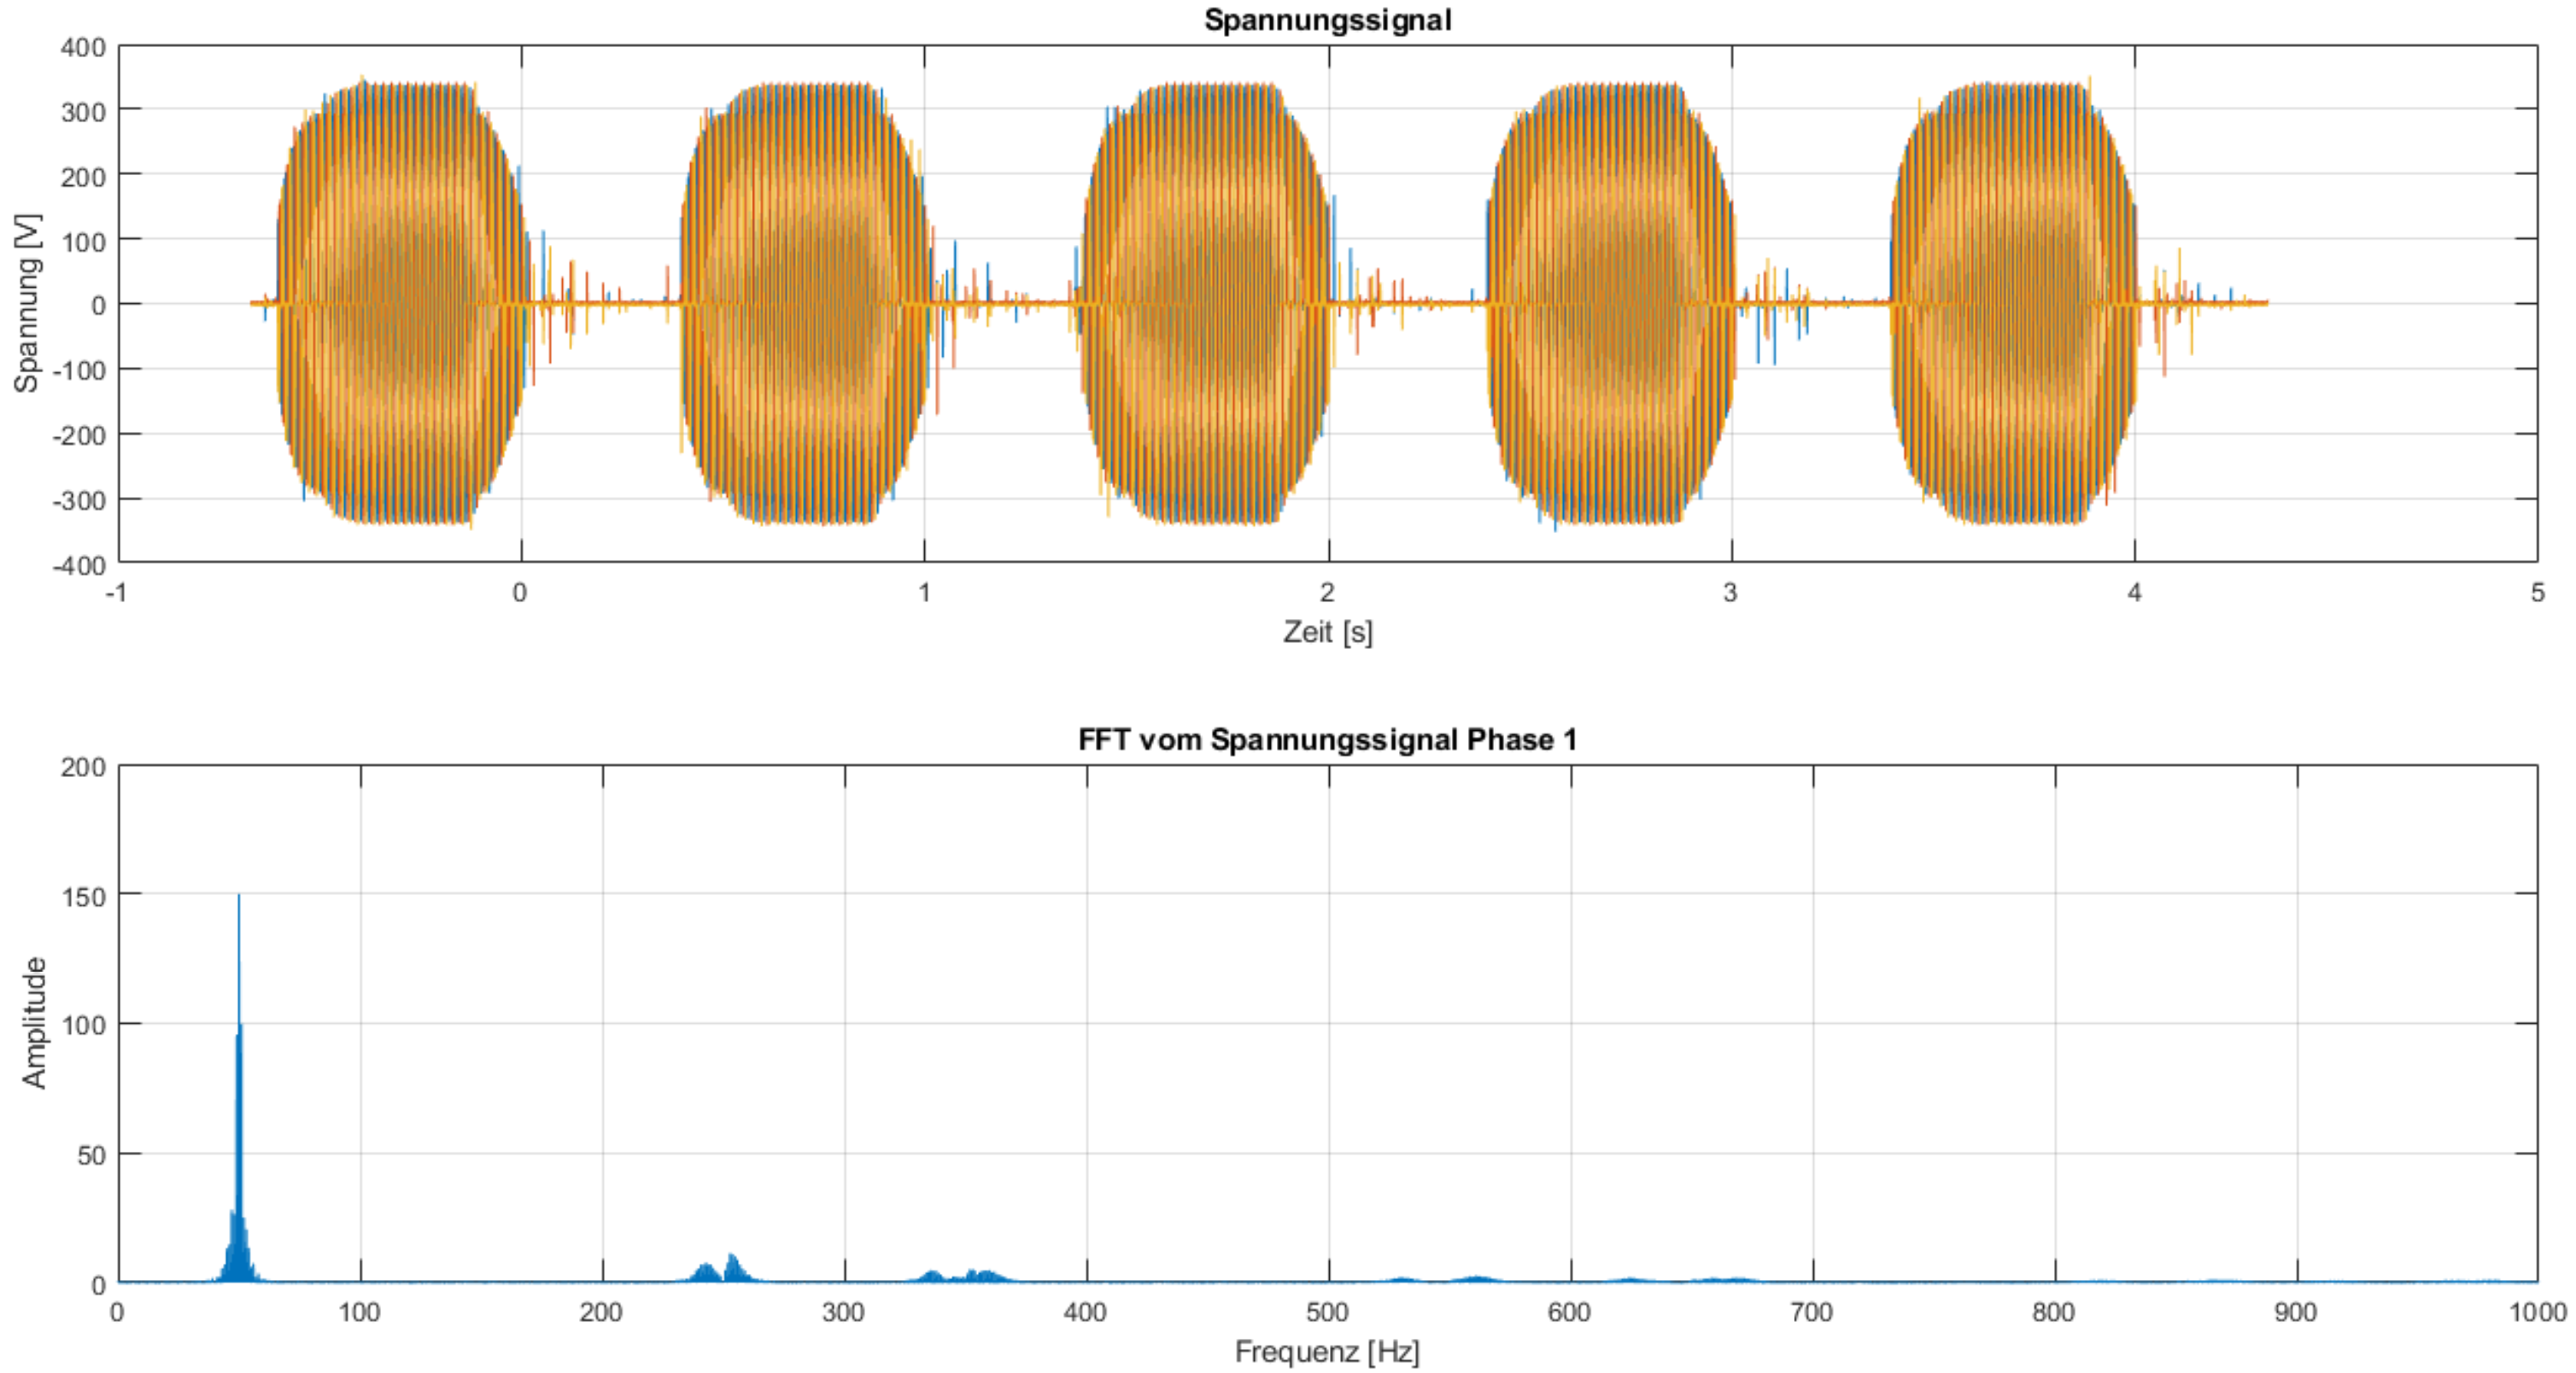
\includegraphics[width=\textwidth]{Messung_Widerstand_Schwing_0_5.png}	
	\caption{Messung mit der Schwingungspaketsteuerung mit einem Duty Cycle von 0.5}\label{fig:Mess_Schwing_50}
\end{figure}


\newpage
\begin{table}[ht!]
	\centering
	\begin{tabular}{|l|l|l|}
		\hline
		Frequenz {[}Hz{]} & Amplitude {[}V{]} & Verhältnis zur Grundschwingung \\ \hline
		46                & 14.7351           & 9.83\%                         \\ \hline
		47                & 28                & 18.68\%                        \\ \hline
		48                & 26.376            & 17.59\%                        \\ \hline
		49                & 95.6              & 63.77\%                        \\ \hline
		50                & 149.92            & 100\%                          \\ \hline
		51                & 99.8              & 66.57\%                        \\ \hline
		52                & 25.134            & 16.76\%                        \\ \hline
		53                & 20.6              & 13.74\%                        \\ \hline
	\end{tabular}
\caption{Amplitudenwerte bei der Frequenzen bei der Schwingungspaketsteuerung mit einem Duty Cycle von 0.5}\label{tab:Mess_Spannung_Schwing_50}
\end{table}

Wie bei den Simulationen im Kapitel \ref{sec:Schwingungspaketsteuerung_Simulation} gezeigt, treten bei der Schwingungspaketsteuerung fast keine harmonische Oberwelle auf. Bei dem FFT erkennt man, dass das Seitenband bei der Grundschwingung relativ breit ist. In der Tabelle \ref{tab:Mess_Spannung_Schwing_50} sind die Werte der Amplituden der Sub- und Zwischenharmonischen aufgelistet. Dabei wurden die Werte aus dem FFT ausgelesen, welche sich in der Nähe der Grundschwingung von \SI{50}{Hz} befinden und eine hohen Amplitudenwert besitzen. \\
Die Werte der Tabelle \ref{tab:Mess_Spannung_Schwing_50} wurden mit denen des FFTs der Plecs-Simulation verglichen. Die Grafik und die Werten der Messung und der Simulation befinden sich im Anhang \ref{sec:Vergleich_Mess_Sim_Schwing_50}. Dabei wurde festgestellt, dass die Kurvenformen der FFT zwar ähnlich aussehen. Bei näherem betrachten gibt es jedoch grosse Unterschiede zwischen den Peak-Werten. In der Simulation schnellen, nach dem Einschalten eines Paketes, die Spannungen sogleich an den Spitzenwert, wobei dies beim Laboraufbau nicht der Fall ist. Deshalb ist bei der Simulation, bei gleicher Zeitdauer, die Spannung länger auf dem Spitzenwert als beim Laboraufbau. Des Weiteren sind alle Bauteile in der Simulation ideal wobei dies in der Praxis nicht der Fall ist. Deshalb ist auch eine minimale Abweichung des Spitzenwertes ersichtlich. Die Standartabweichung aller aufgeführten Frequenzen beträgt: 7.912. Dieser Wert wurde mit Excel berechnet wobei die Frequenzen als Stichprobe verwendet wurden. 


\newpage
\subsubsection*{Schwingungspaketsteuerung mit Duty Cycle von 0.8}
In der Abbildung \ref{fig:Mess_Schwing_80} ist die Schwingungspaketsteuerung mit einem Duty Cycle von 0.8 ersichtlich.
\begin{figure}[ht!]
	\centering
	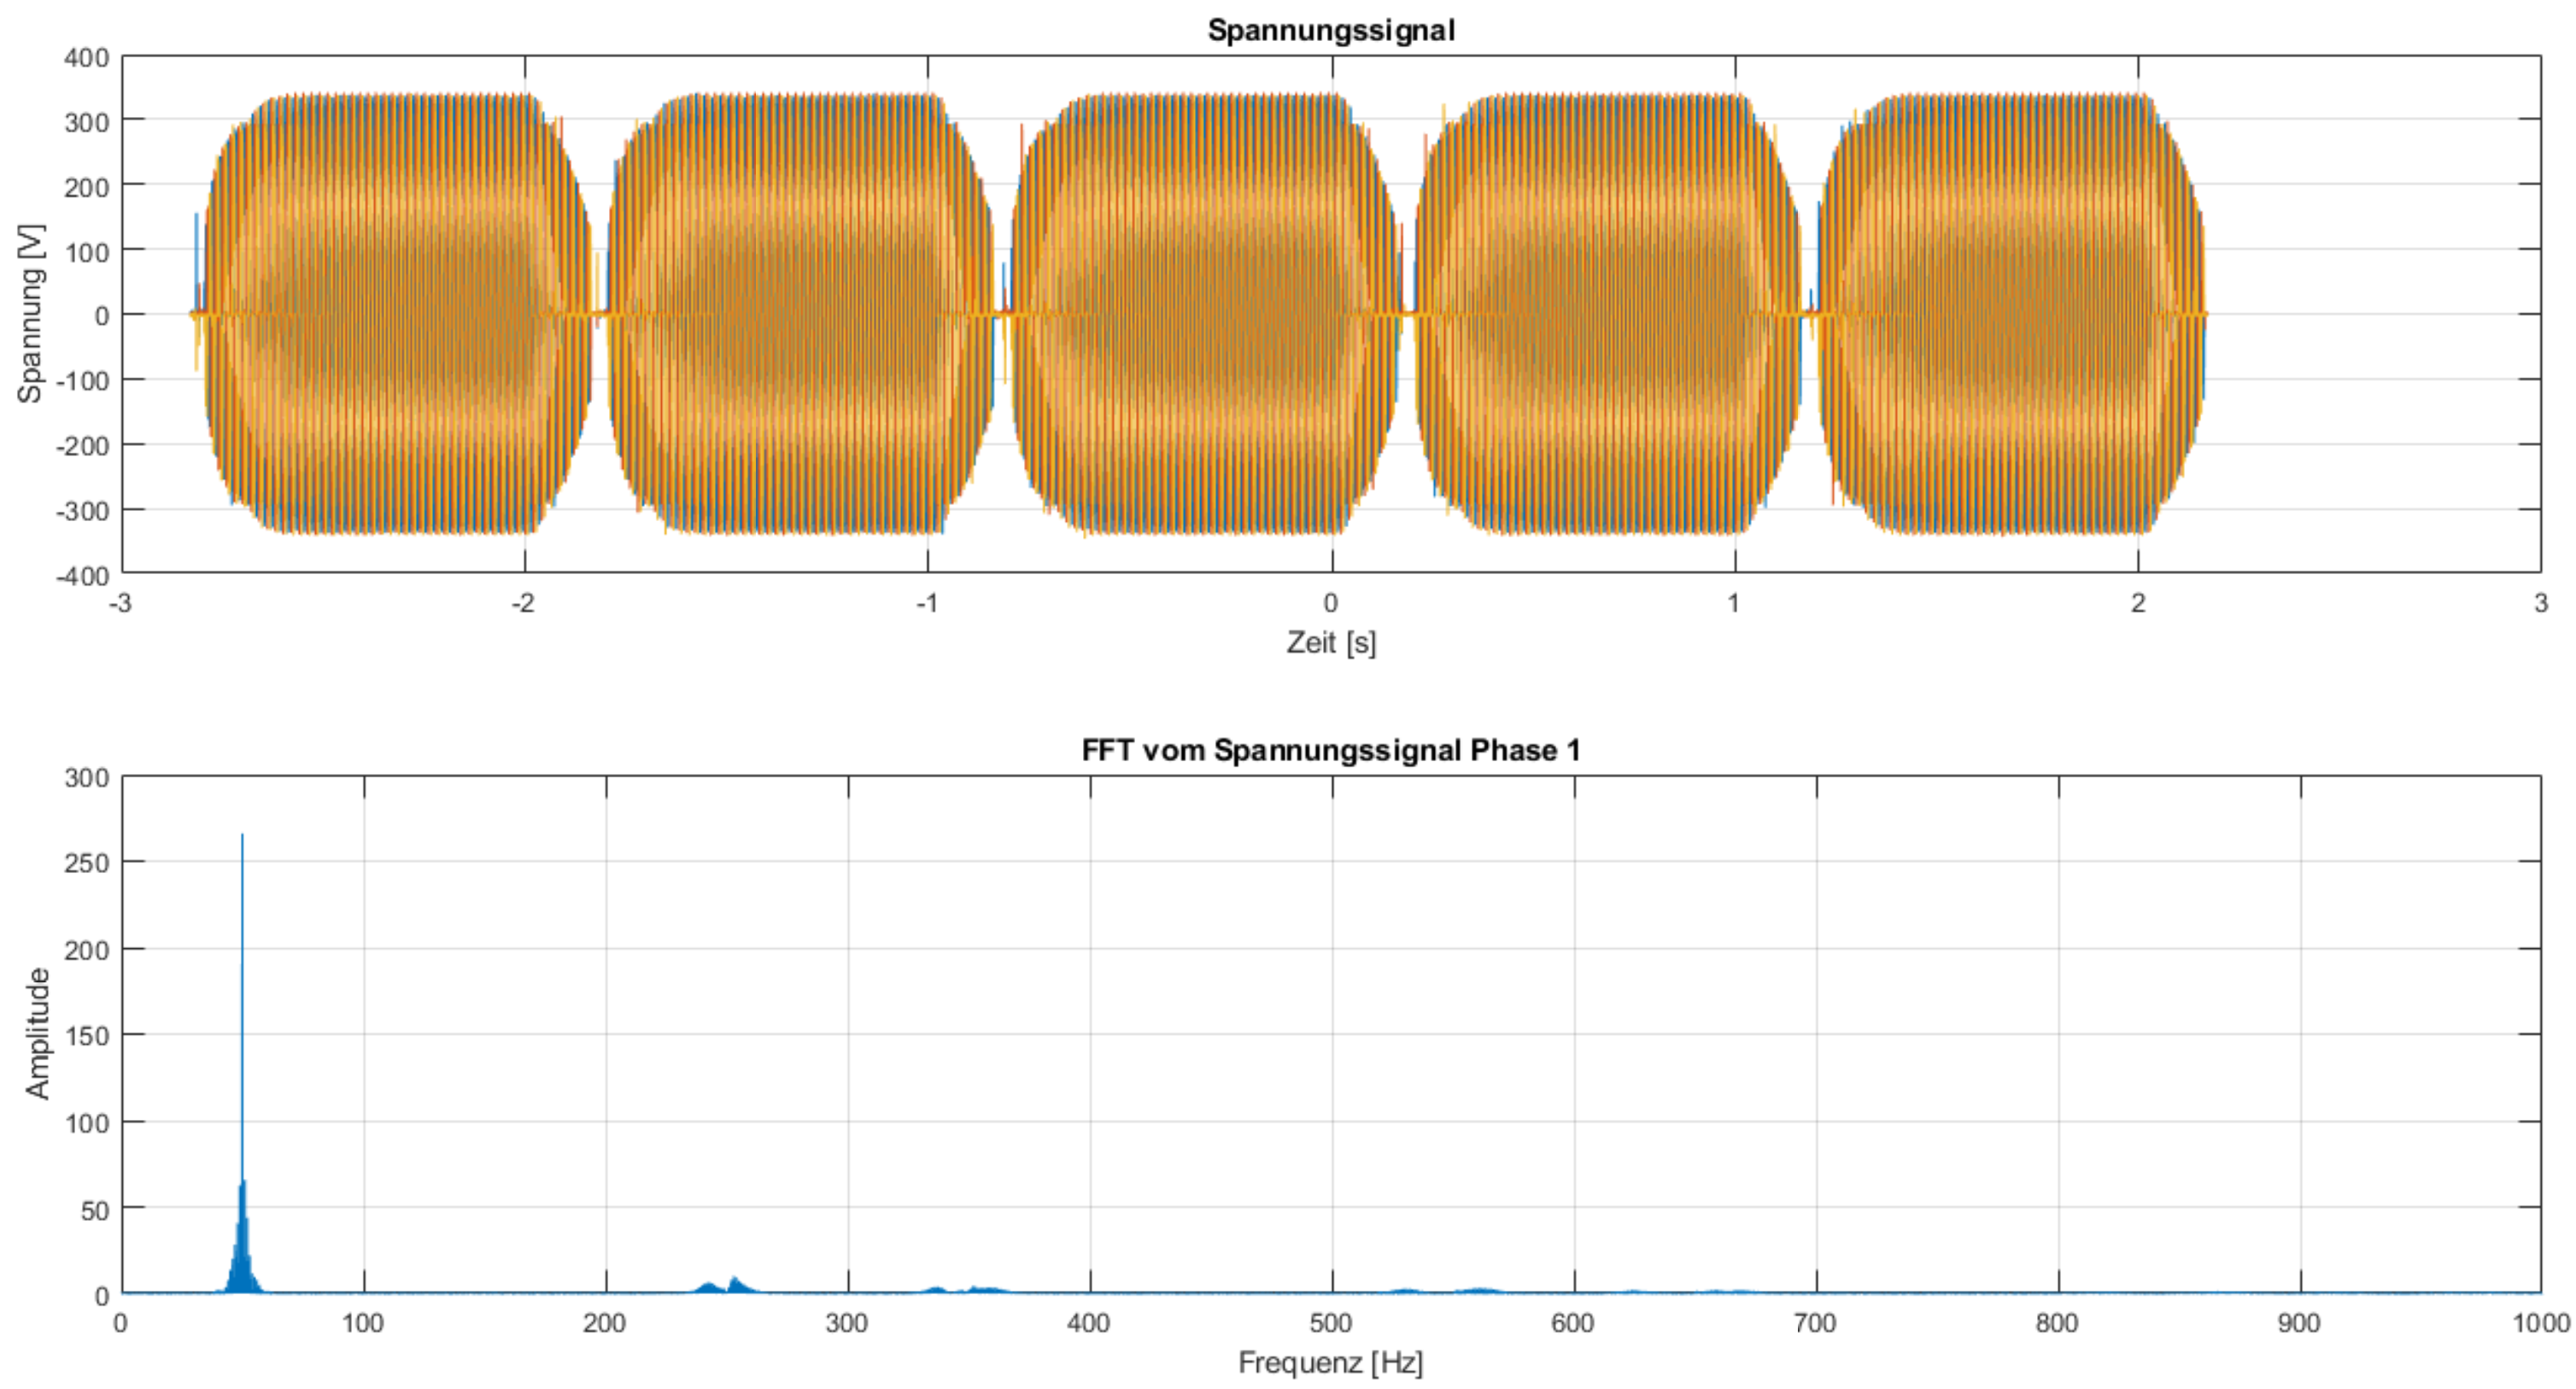
\includegraphics[width=\textwidth]{Messung_Widerstand_Schwing_0_8.png}	
	\caption{Messung mit der Schwingungspaketsteuerung mit einem Duty Cycle von 0.8}\label{fig:Mess_Schwing_80}
\end{figure}


\begin{table}[ht!]
	\centering
	\begin{tabular}{|l|l|l|}
		\hline
		Frequenz {[}Hz{]} & Amplitude {[}V{]} & Verhältnis zur Grundschwingung \\ \hline
		46                & 20.173            & 7.58\%                         \\ \hline
		47                & 28.26             & 10.62\%                        \\ \hline
		48                & 40.576            & 15.26\%                        \\ \hline
		49                & 62.694            & 23.57\%                        \\ \hline
		50                & 265.98            & 100\%                          \\ \hline
		51                & 65.7              & 24.7\%                         \\ \hline
		52                & 43.812            & 16.47\%                        \\ \hline
		53                & 21.939            & 8.25\%                         \\ \hline
	\end{tabular}
\caption{Amplitudenwerte bei der Frequenzen bei Schwingungspaket 80\%}\label{tab:Mess_Spannung_Schwing_80}
\end{table}

Anders als beim Schwingungspaket mit einem Duty Cycle von 0.5, ist bei 0.8 der Peak bei der Grundfrequenz von von \SI{50}{Hz} deutlich höher. Das kommt davon, da die Spannung einen längere Zeit auf dem Maximum ist.
In der Tabelle \ref{tab:Mess_Spannung_Schwing_80} befinden sich die Werten der Amplituden und deren Verhältnis zur Grundschwingung.\\
Wie bei der Schwingungspaketsteuerung mit Duty Cycle von 0.5 wurden auch die Resultate der Messung mit 0.8, mit der Simulation verglichen. Die Tabelle mit den Werten und der grafische Vergleich befindet sich im Anhang \ref{sec:Vergleich_Mess_Sim_Schwing_80}. Auch hier gab es Abweichungen bei den verschiedenen Frequenzen zwischen der Simulation und der Messung. Diese waren jedoch bedeutend kleiner als bei der anderen Schwingungspaketsteuerung. Es resultierte eine Standartabweichung von 2.481. Als Grund, für eine niedrigere Abweichung ist, dass die Schwingungspakete eine längere Zeit auf dem Maximum bleiben. Das Hoch- und Herunterfahren haben somit einen kleineren Einfluss auf die Amplitudenwerte. Deshalb ist eine grössere Ähnlichkeit zur Simulation ersichtlich.



\newpage
\subsubsection*{Hartes Auf- und Absteuern}
Die Abbildung \ref{fig:Mess_Sanft} zeigt, ein hartes Auf- und Absteuern der Spannung.

\begin{figure}[ht!]
	\centering
	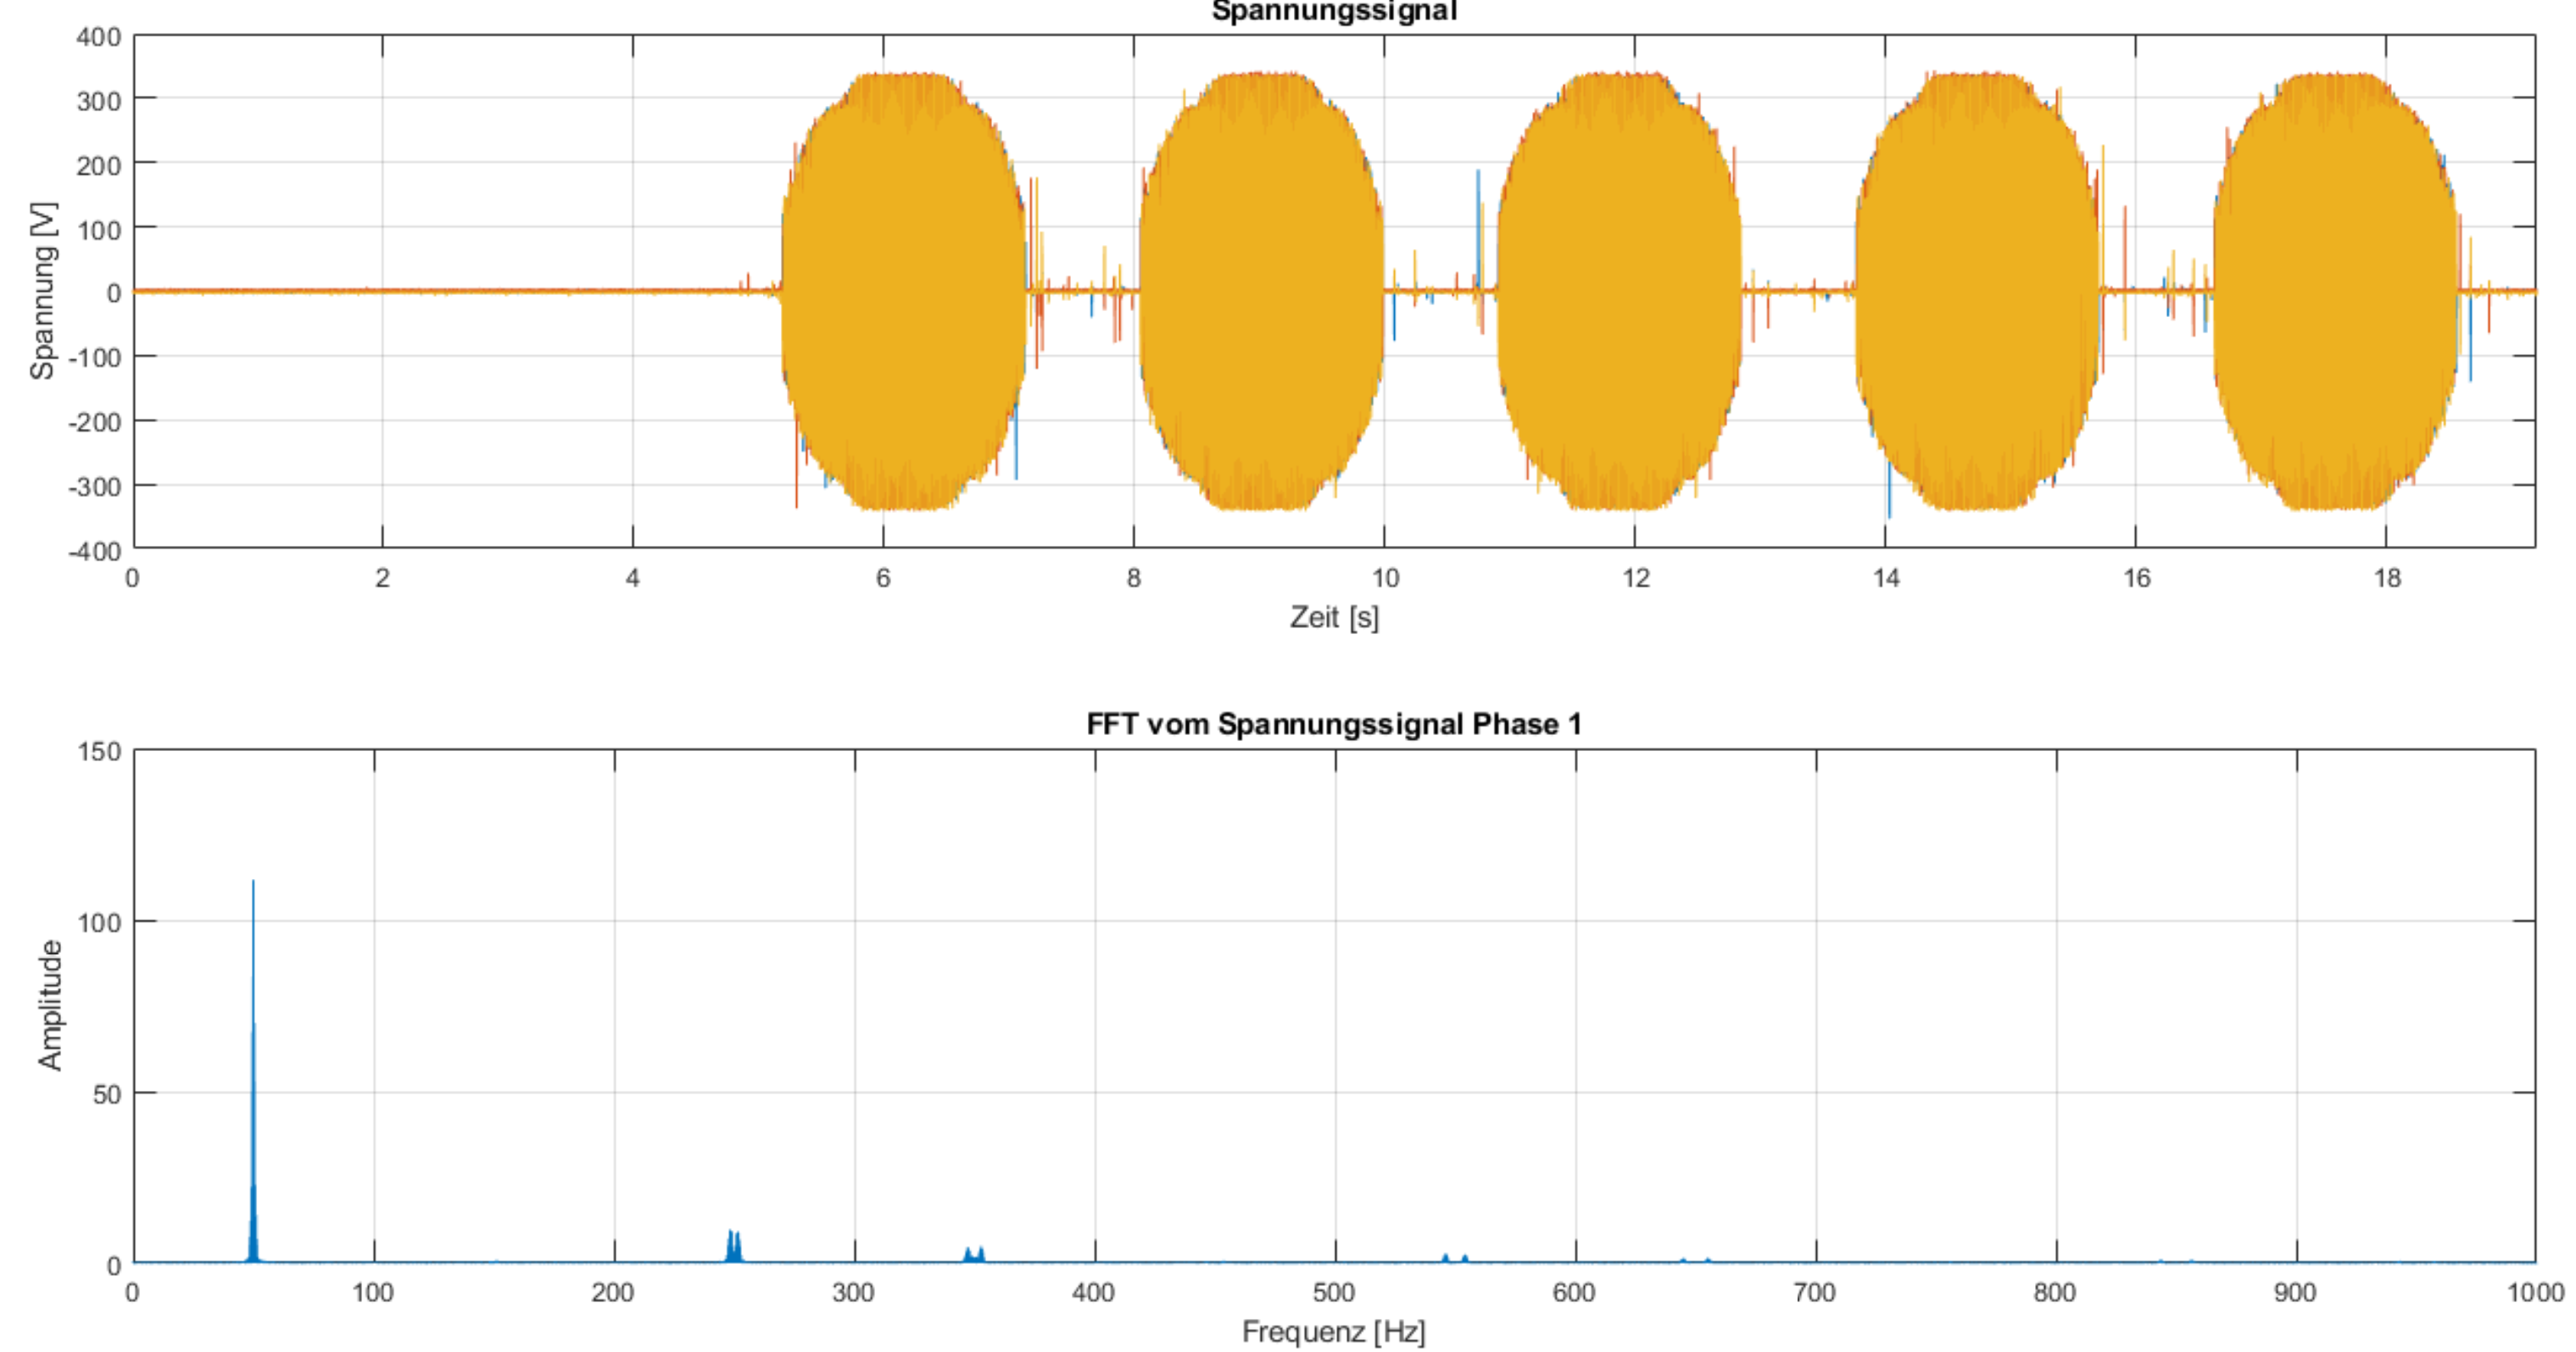
\includegraphics[width=\textwidth]{Mess_Widerstand_AufAb.png}	
	\caption{Messung mit Auf- und Absteuern}\label{fig:Mess_Sanft}
\end{figure}


\begin{table}[ht!]
	\centering
	\begin{tabular}{|l|l|l|}
		\hline
		Frequenz {[}Hz{]} & Amplitude {[}V{]} & Verhältnis zur Grundschwingung \\ \hline
		49.65             & 67.126            & 60.11\%                        \\ \hline
		49.7              & 40.9583           & 36.68\%                        \\ \hline
		50                & 111.6763          & 100\%                          \\ \hline
		50.05             & 58.2021           & 52.12\%                        \\ \hline
		50.35             & 70.0651           & 62.74\%                        \\ \hline
		249               & 9.0297            & 8.09\%                         \\ \hline
		250               & 1.0487            & 0.94\%                         \\ \hline
		251 		      & 1.8206            & 1.63\%                         \\ \hline
	\end{tabular}
\caption{Amplitudenwerte bei der Frequenzen bei hartes Auf- und Absteuern}\label{tab:Mess_Spannung_AufAb_hart}
\end{table}

Für die Tabelle \ref{tab:Mess_Spannung_AufAb_hart} wurden die höchsten Amplitudenwerte bei der Grundschwingung von \SI{50}{Hz} und bei der 5. Harmonische bei \SI{250}{Hz} aufgelistet.
Wie auch bei den Schwingungspaketsteuerungen, tritt bei dem harten Auf- und Absteuern die harmonischen Oberschwingung praktisch nicht mehr auf. Jedoch sind auch hier sub- und zwischenharmonische Oberwellen ersichtlich. Diese betragen bei den Frequenzen \SI{49.65}{Hz} und \SI{50.35}{Hz} über 60\% der Grundschwingung. Bei dem Vergleich des harten Auf- und Absteuern im Laboraufbau und der Simulation wurde ein Unterschied der Signaldauer erkannt. Während bei der Simulation das Auffahren \SI{0.2}{s} dauert, benötigt der Laboraufbau mit fast \SI{0.8}{s}, deutlich länger. Da der Thyristorsteller nicht schneller reagiert, dauerte es fast \SI{1}{s} bis das nächste Paket eingeschaltet wird. Diese Gründe erklären den grossen Unterschied zwischen dem FFT der Simulation und der Messung. Im Kapitel \ref{sec:sanftes_hoch_und_runterfahren} wird das Verhalten von verschieden Anstiegs-Funktionen und die dazu gehörigen FFTs erklärt. Berechnet wurde eine Standartabweichung von 19.812 wobei dieser Wert 2.5 mal gross ist, wie die Standartabweichung des Schwingungspaketes mit einem Duty Cycle von 0.5. Der Vergleich mit der Simulation ist im Anhang im Kapitel \ref{sec:Vergleich_Mess_Sim_hart_AufAb} ersichtlich.

\newpage
\subsubsection*{Sanftes Auf- und Absteuern}
Die Abbildung \ref{fig:Mess_Sanft_langsam} zeigt, ein sanftes Auf- und Absteuern der Spannung.


\begin{figure}[ht!]
	\centering
	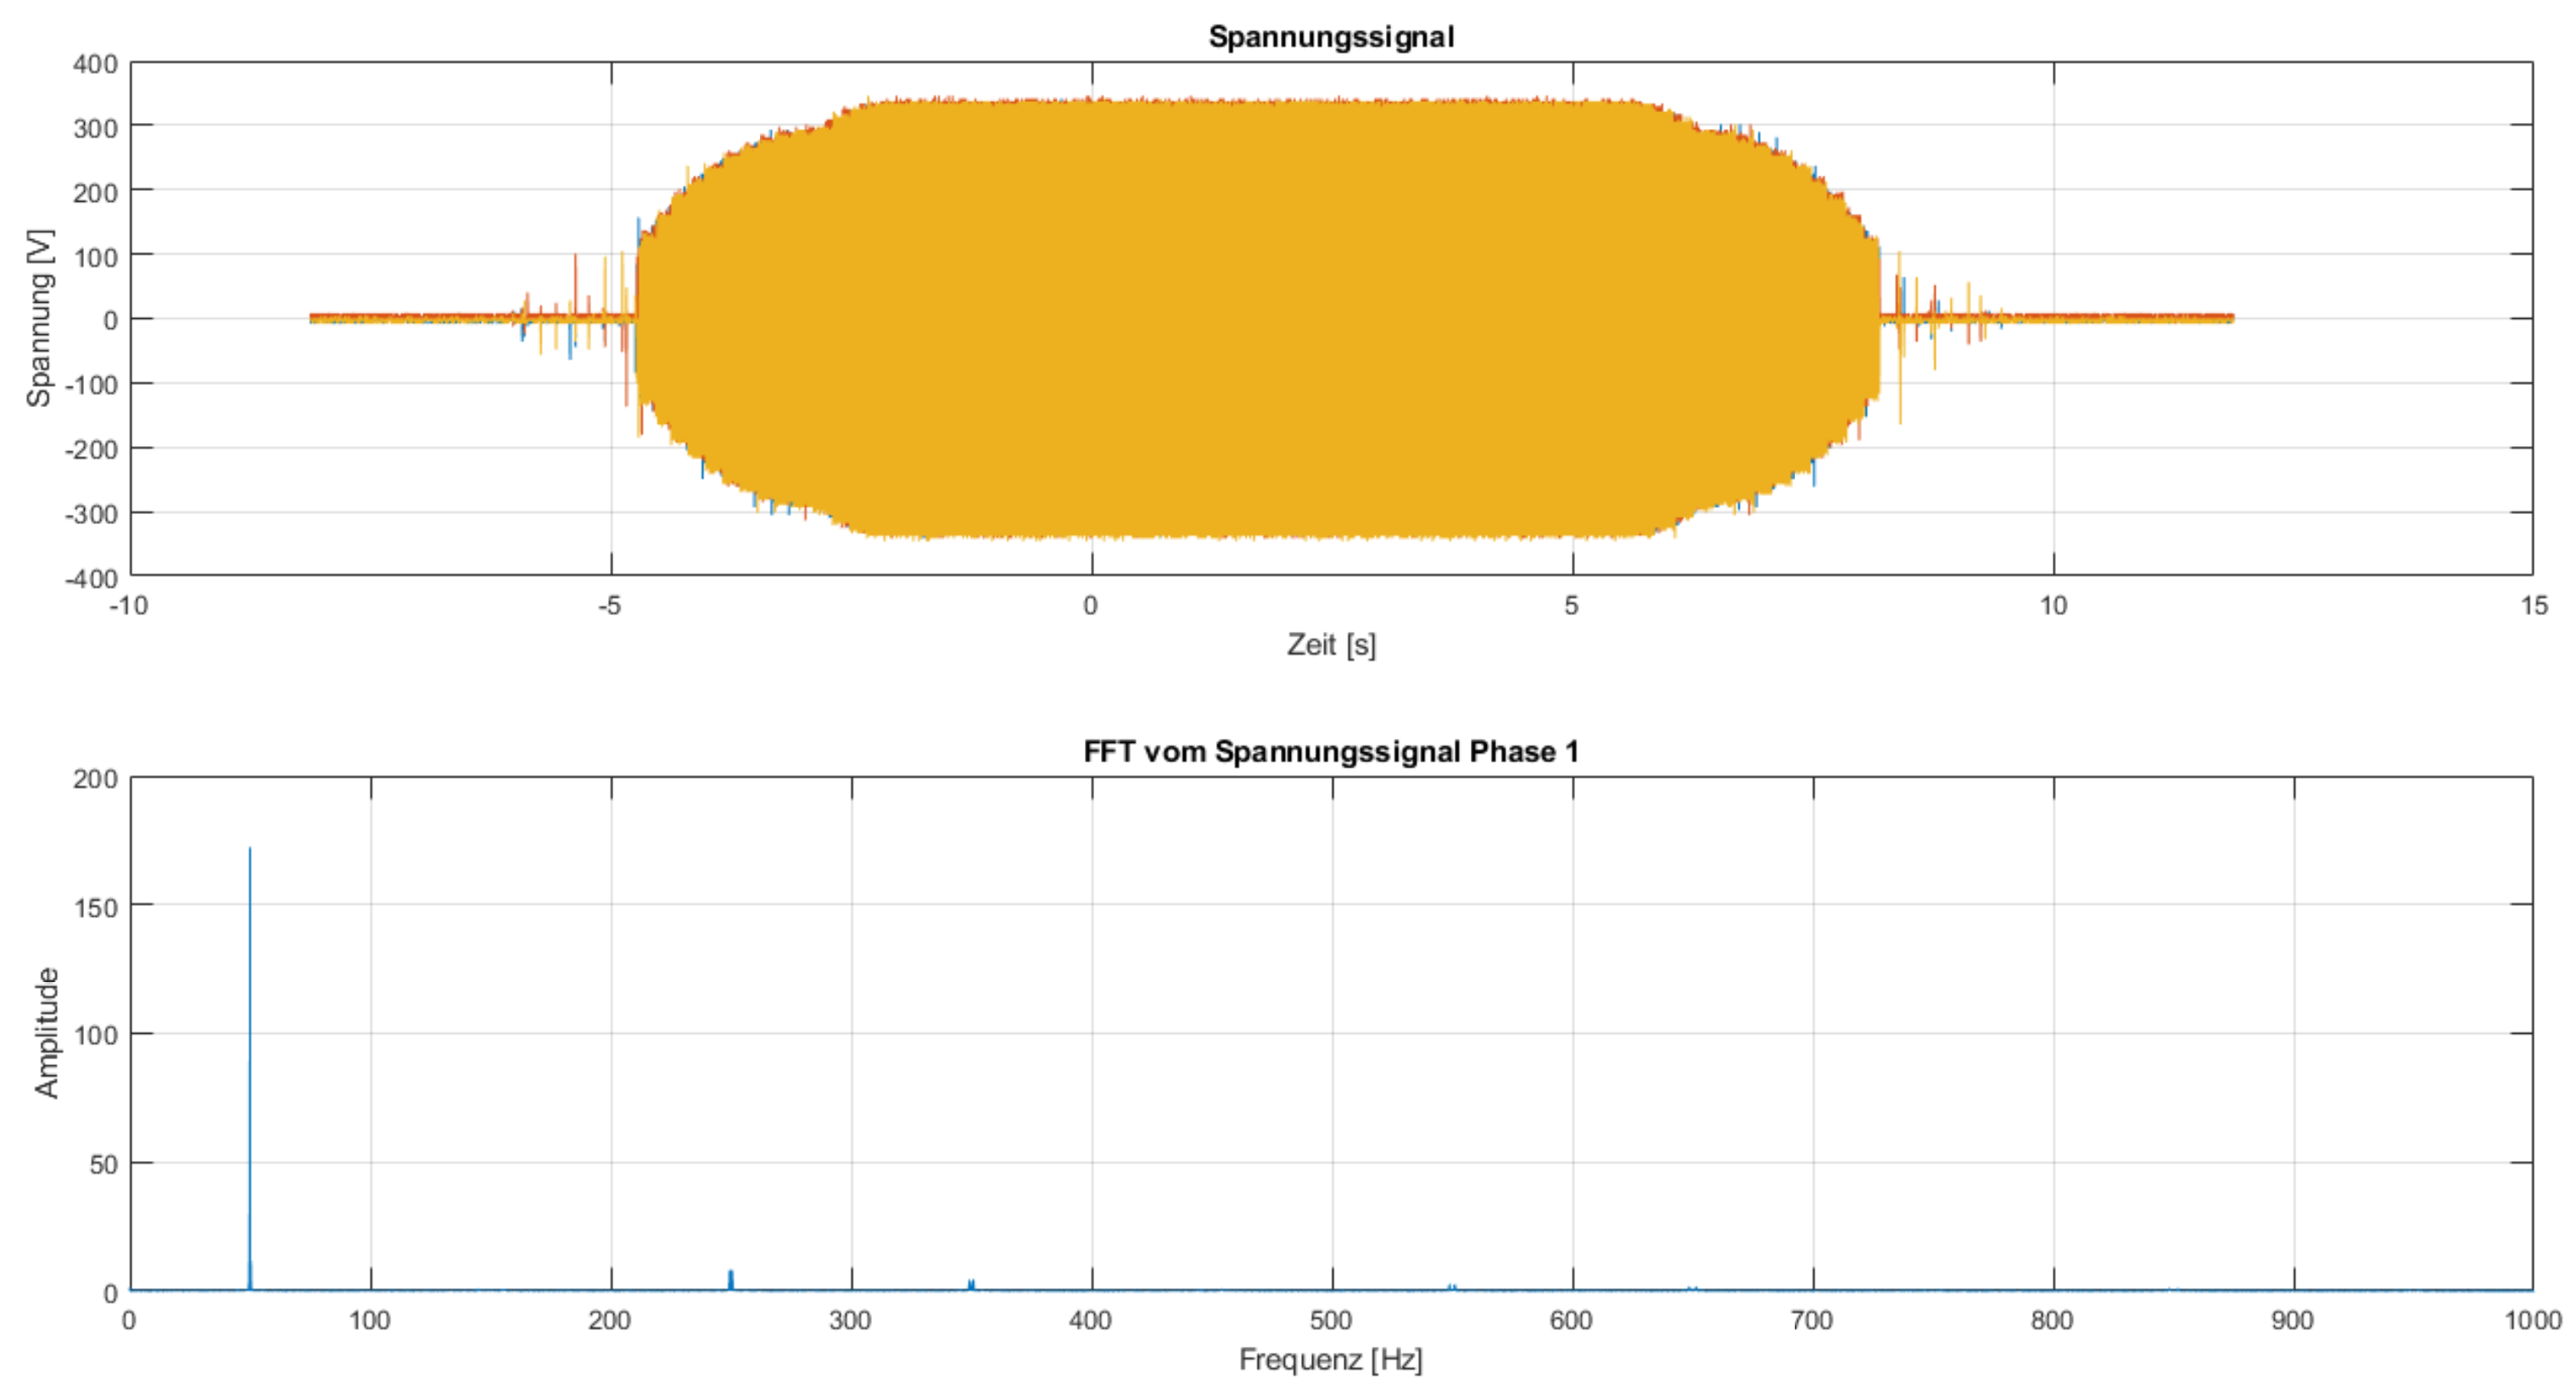
\includegraphics[width=\textwidth]{Messung_Widerstand_Sanft_langsam.png}	
	\caption{Messung mit sanftem Auf- und Absteuern}\label{fig:Mess_Sanft_langsam}
\end{figure}


\begin{table}[ht!]
	\centering
	\begin{tabular}{|l|l|l|}
		\hline
		Frequenz {[}Hz{]} & Amplitude {[}V{]} & Verhältnis zur Grundschwingung \\ \hline
		49.8              & 18.522            & 10.75\%                        \\ \hline
		49.85             & 26.576            & 15.43\%                        \\ \hline
		49.9              & 29.507            & 17.131\%                       \\ \hline
		49.95             & 91.266            & 52.99\%                        \\ \hline
		50                & 172.241           & 100\%                          \\ \hline
		50.05             & 116.719           & 67.76\%                        \\ \hline
		50.1              & 28.629            & 16.62\%                        \\ \hline
		50.15             & 30.076            & 17.46\%                        \\ \hline
		50.2              & 18.72             & 10.87\%                        \\ \hline
		249.6             & 8.183             & 4.75\%                         \\ \hline
		250               & 1.158             & 0.67\%                         \\ \hline
		250.4             & 7.466             & 4.33\%                         \\ \hline
	\end{tabular}
\caption{Amplitudenwerte bei der Frequenzen beim sanften Auf- und Absteuern}\label{tab:Mess_Spannung_AufAb_sanft}
\end{table}

Im visuellen Vergleich mit dem hartem Auf- und Abfahren zeigt das FFT, dass die Frequenzbänder dünner und der Peak bei \SI{50}{Hz} grösser geworden sind. In der Tabelle \ref{tab:Mess_Spannung_AufAb_sanft} sind die höchsten Amplitudenwerte der Frequenzen, die sich in der Nähe der Grundschwingung von \SI{50}{Hz} und der 5. Harmonischen bei \SI{250}{Hz} aufhalten, aufgelistet. Der Vergleich mit der Simulation, welches sich im Anhang \ref{sec:Vergleich_Mess_Sim_sanft_AufAb} befindet, zeigt eine grossen Unterschiede der Amplitudenwerte auf. Ein Grund dafür ist, dass die Simulation für das Hoch- und Runterfahren eine Zeitdauer von \SI{0.3}{s} benötigt, wobei sie bei der Messung \SI{3}{s} beträgt. Zusätzlich ist bei der Simulation während \SI{6}{s} die Spannung auf dem Spitzenwert, beim Laboraufbau sind es jedoch \SI{7}{s}.  Berechnet wurde für die Standartabweichung ein Wert von 88.904. Es ist ersichtlich, dass die beiden Funktionen nicht miteinander verglichen werden können, da die Abweichung zu gross ist.


\subsubsection{Messungen Asynchronmaschine}

Auch bei der Asynchronmaschine wurden die verschiedenen Ansteuerungsarten, Phasenanschnitt mit 60\textdegree \hspace{0.02cm} und 90\textdegree \hspace{0.02cm}, Schwingungspaket mit Duty Cycle von 0.5 und 0.8 und dem harte und sanfte Auf- und Absteuern durchgeführt. Dabei stellte man fest, dass sich die Schwingungspaketsteuerungen und das harte Auf- und Absteuern nicht für einen Asynchronmotor eignen. Der Motor fährt zu schnell Hinauf und Hinunter und befindet sich nie in einem geeigneten Stationären Zustand. Deshalb verzichtete man bei der Messung auf diese Verfahren. Der Aufbau der Abbildungen und Tabellen ist gleich wie bei dem Widerstand.

\subsubsection*{Phasenanschnitt 60\textdegree}

Bei der Abbildung \ref{fig:Mess_ASM_Phas60} verwendete man einen Phasenanschnittswinkel von 60\textdegree.

\begin{figure}[ht!]
	\centering
	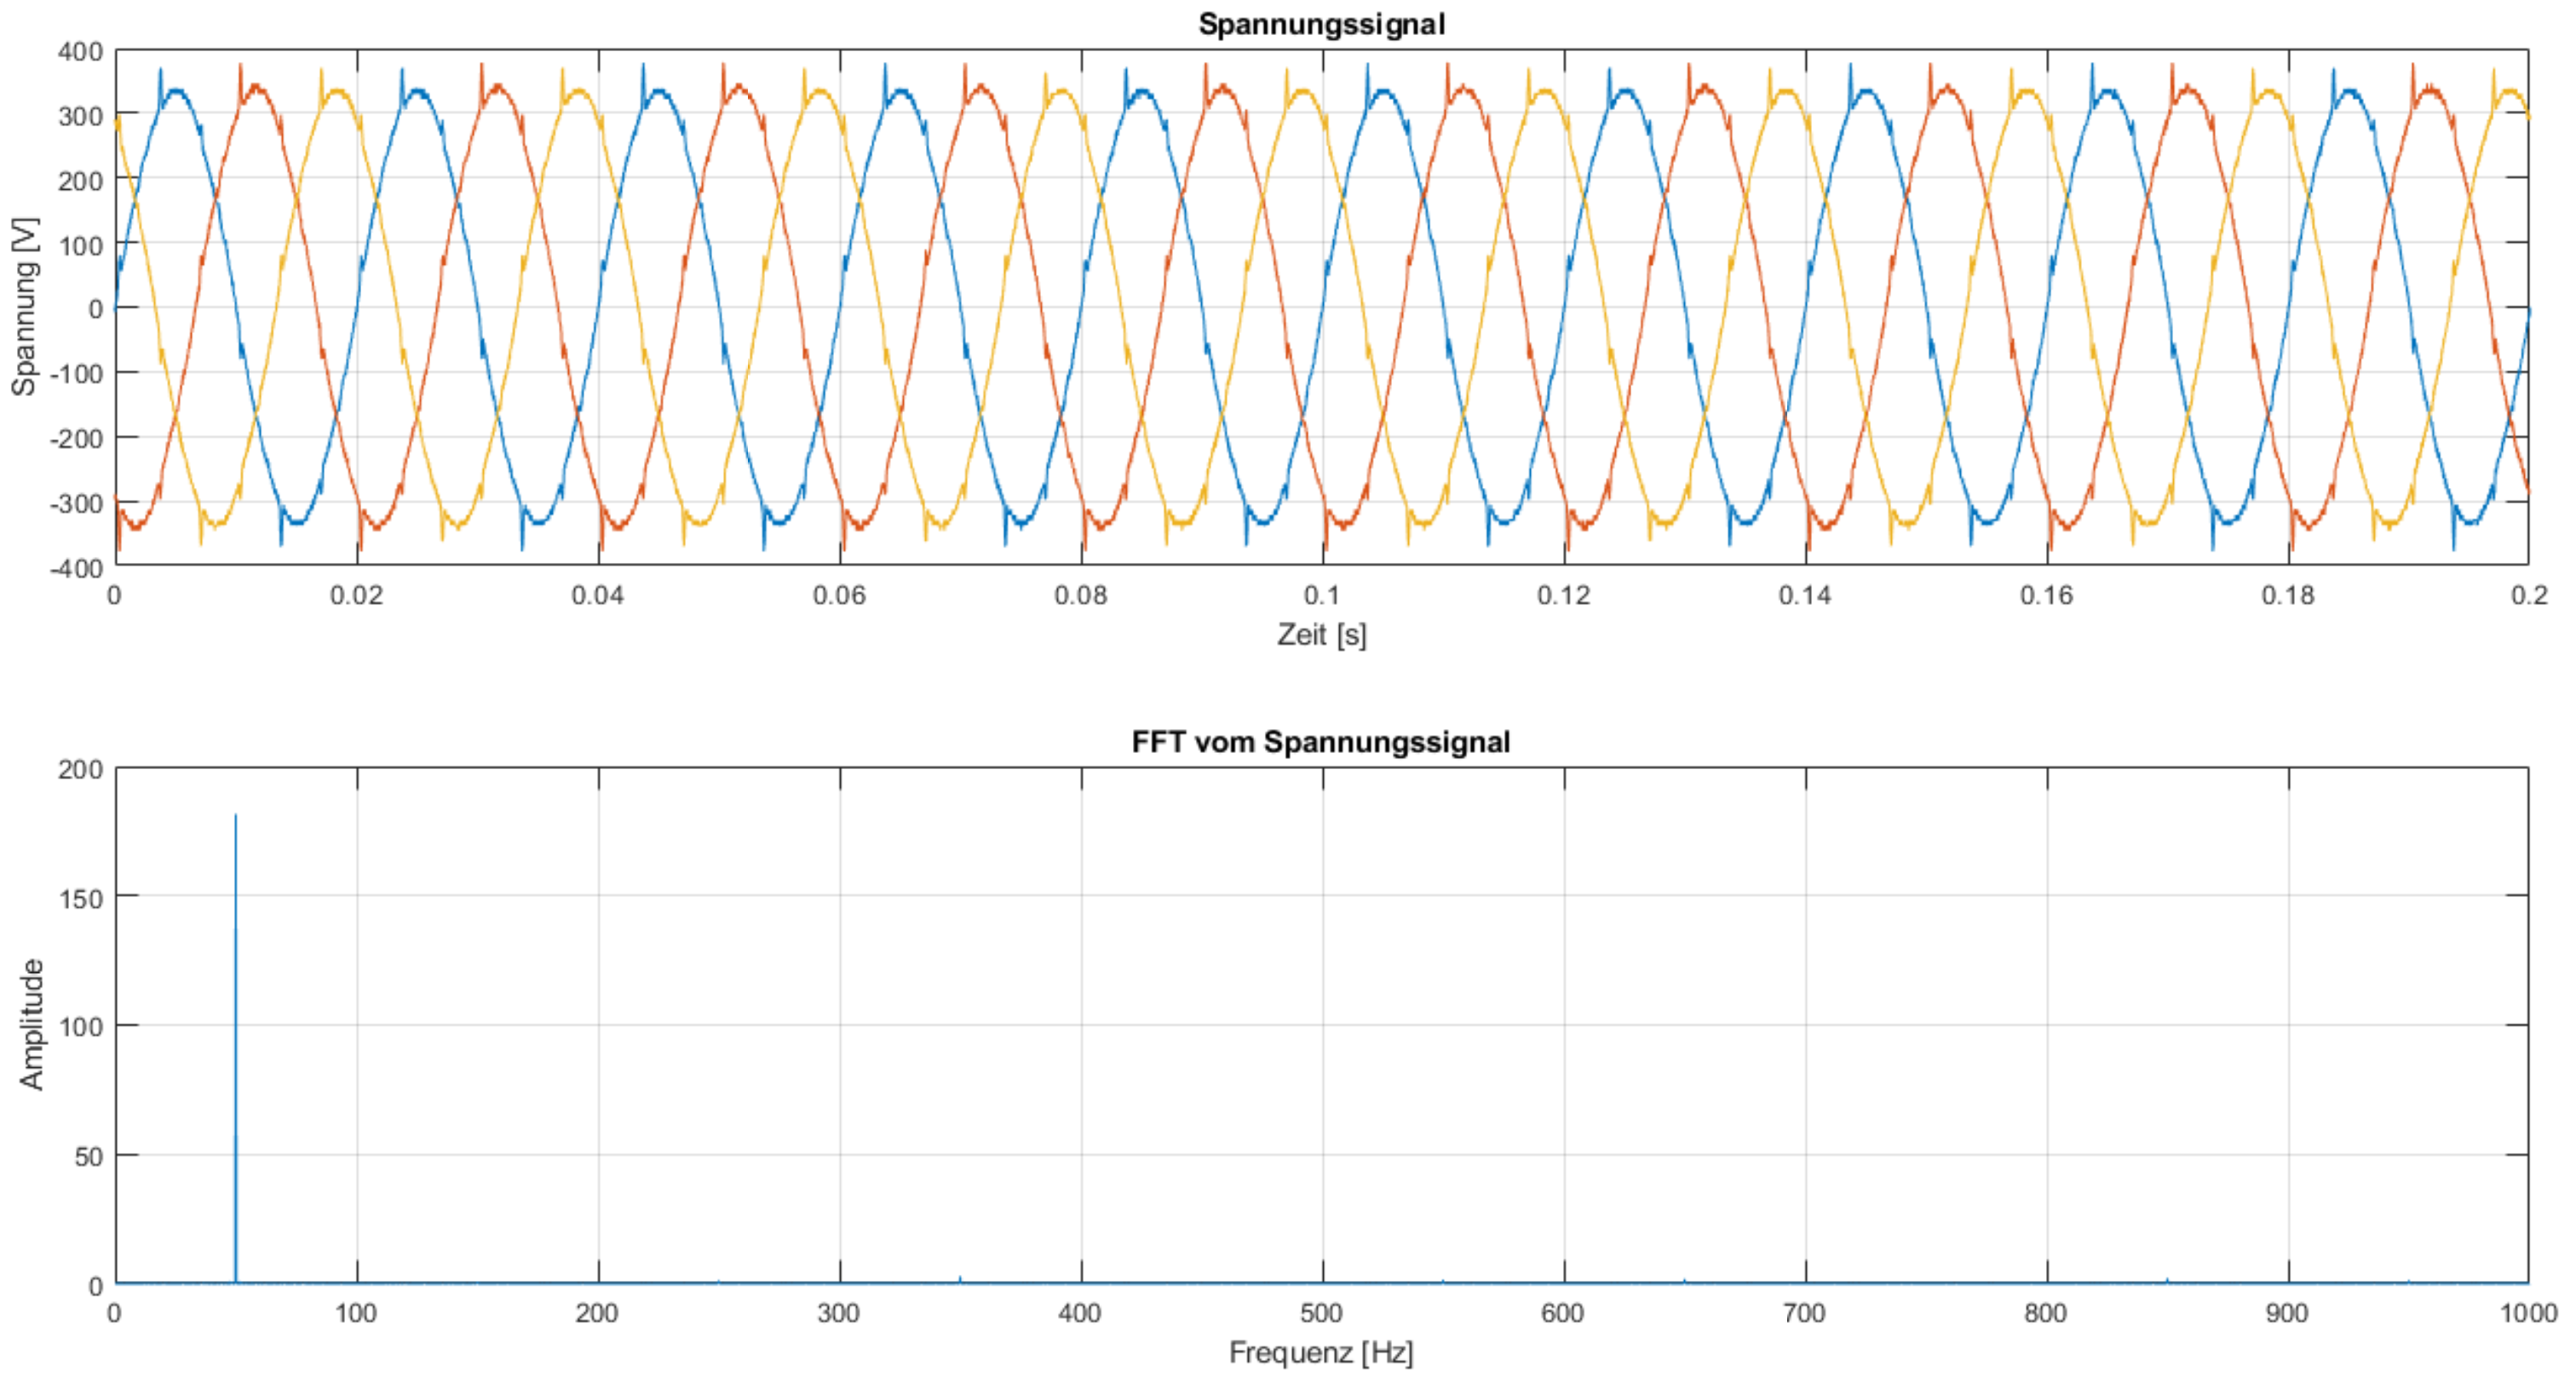
\includegraphics[width=\textwidth]{Messung_ASM_Phas_60grad.png}	
	\caption{Messung mit Phasenanschnitt 60\textdegree}\label{fig:Mess_ASM_Phas60}
\end{figure}


\newpage
\begin{table}[ht!]
	\centering
	\begin{tabular}{|l|l|l|}
		\hline
		Oberschwingungsordnung & Amplitude {[}V{]} & Verhältnis zur Grundschwingung \\ \hline
		1                      & 181.5519          & 100\%                          \\ \hline
		5                      & 1.1065            & 0.61\%                         \\ \hline
		7                      & 2.8728            & 1.58\%                         \\ \hline
		11                     & 1.4537            & 0.8\%                          \\ \hline
	\end{tabular}
\caption{Amplitudenwerte bei der Frequenzen bei Phasenanschnitt 60\textdegree}\label{tab:Mess_Spannung_ASM_Phas60}
\end{table}

Anders als beim Phasenanschnitt von 60\textdegree\hspace{0.02cm} mit dem ohmschen Widerstand, treten bei dem Asynchronmotor fast keine harmonischen Oberschwingungen auf. Da diese Peaks im FFT nicht ersichtlich sind, wurden die Amplituden der Oberschwingungen bis zur 11. Ordnung in der Tabelle \ref{tab:Mess_Spannung_ASM_Phas60} aufgeführt. 
Beim Ansteuern mit dem Winkel von 60\textdegree \hspace{0.02cm} wurde bemerkt, dass die Maschine bereits mit maximaler Drehzahl dreht. Es macht bei den Spannungssignalen keinen Unterschied ob die ASM mit einem Winkel von 60\textdegree \hspace{0.02cm} oder 0\textdegree \hspace{0.02cm} angesteuert wird. Anders als beim Phasenanschnitt mit 60\textdegree\hspace{0.02cm} bei ohmscher Last, sind mit dem gleichen Anschnitswinkel bei der ASM keine Sub- und Zwischenharmonische in der Nähe der Grundfrequenz ersichtlich. Im Verhältnis zur Grundschwingung hat die 7. Ordnung die maximale Abweichung von 1.58\%. Die Werte der harmonischen Schwingungen halten somit die Normen in der Tabelle \ref{tab:kompatibilitätsstufen} ein. 

\newpage
\subsubsection*{Phasenanschnitt 90\textdegree}
Die Abbildung \ref{fig:Mess_ASM_Phas90} zeigt eine Steuerung mit einem Phasenanschnitt von 90\textdegree.

\begin{figure}[ht!]
	\centering
	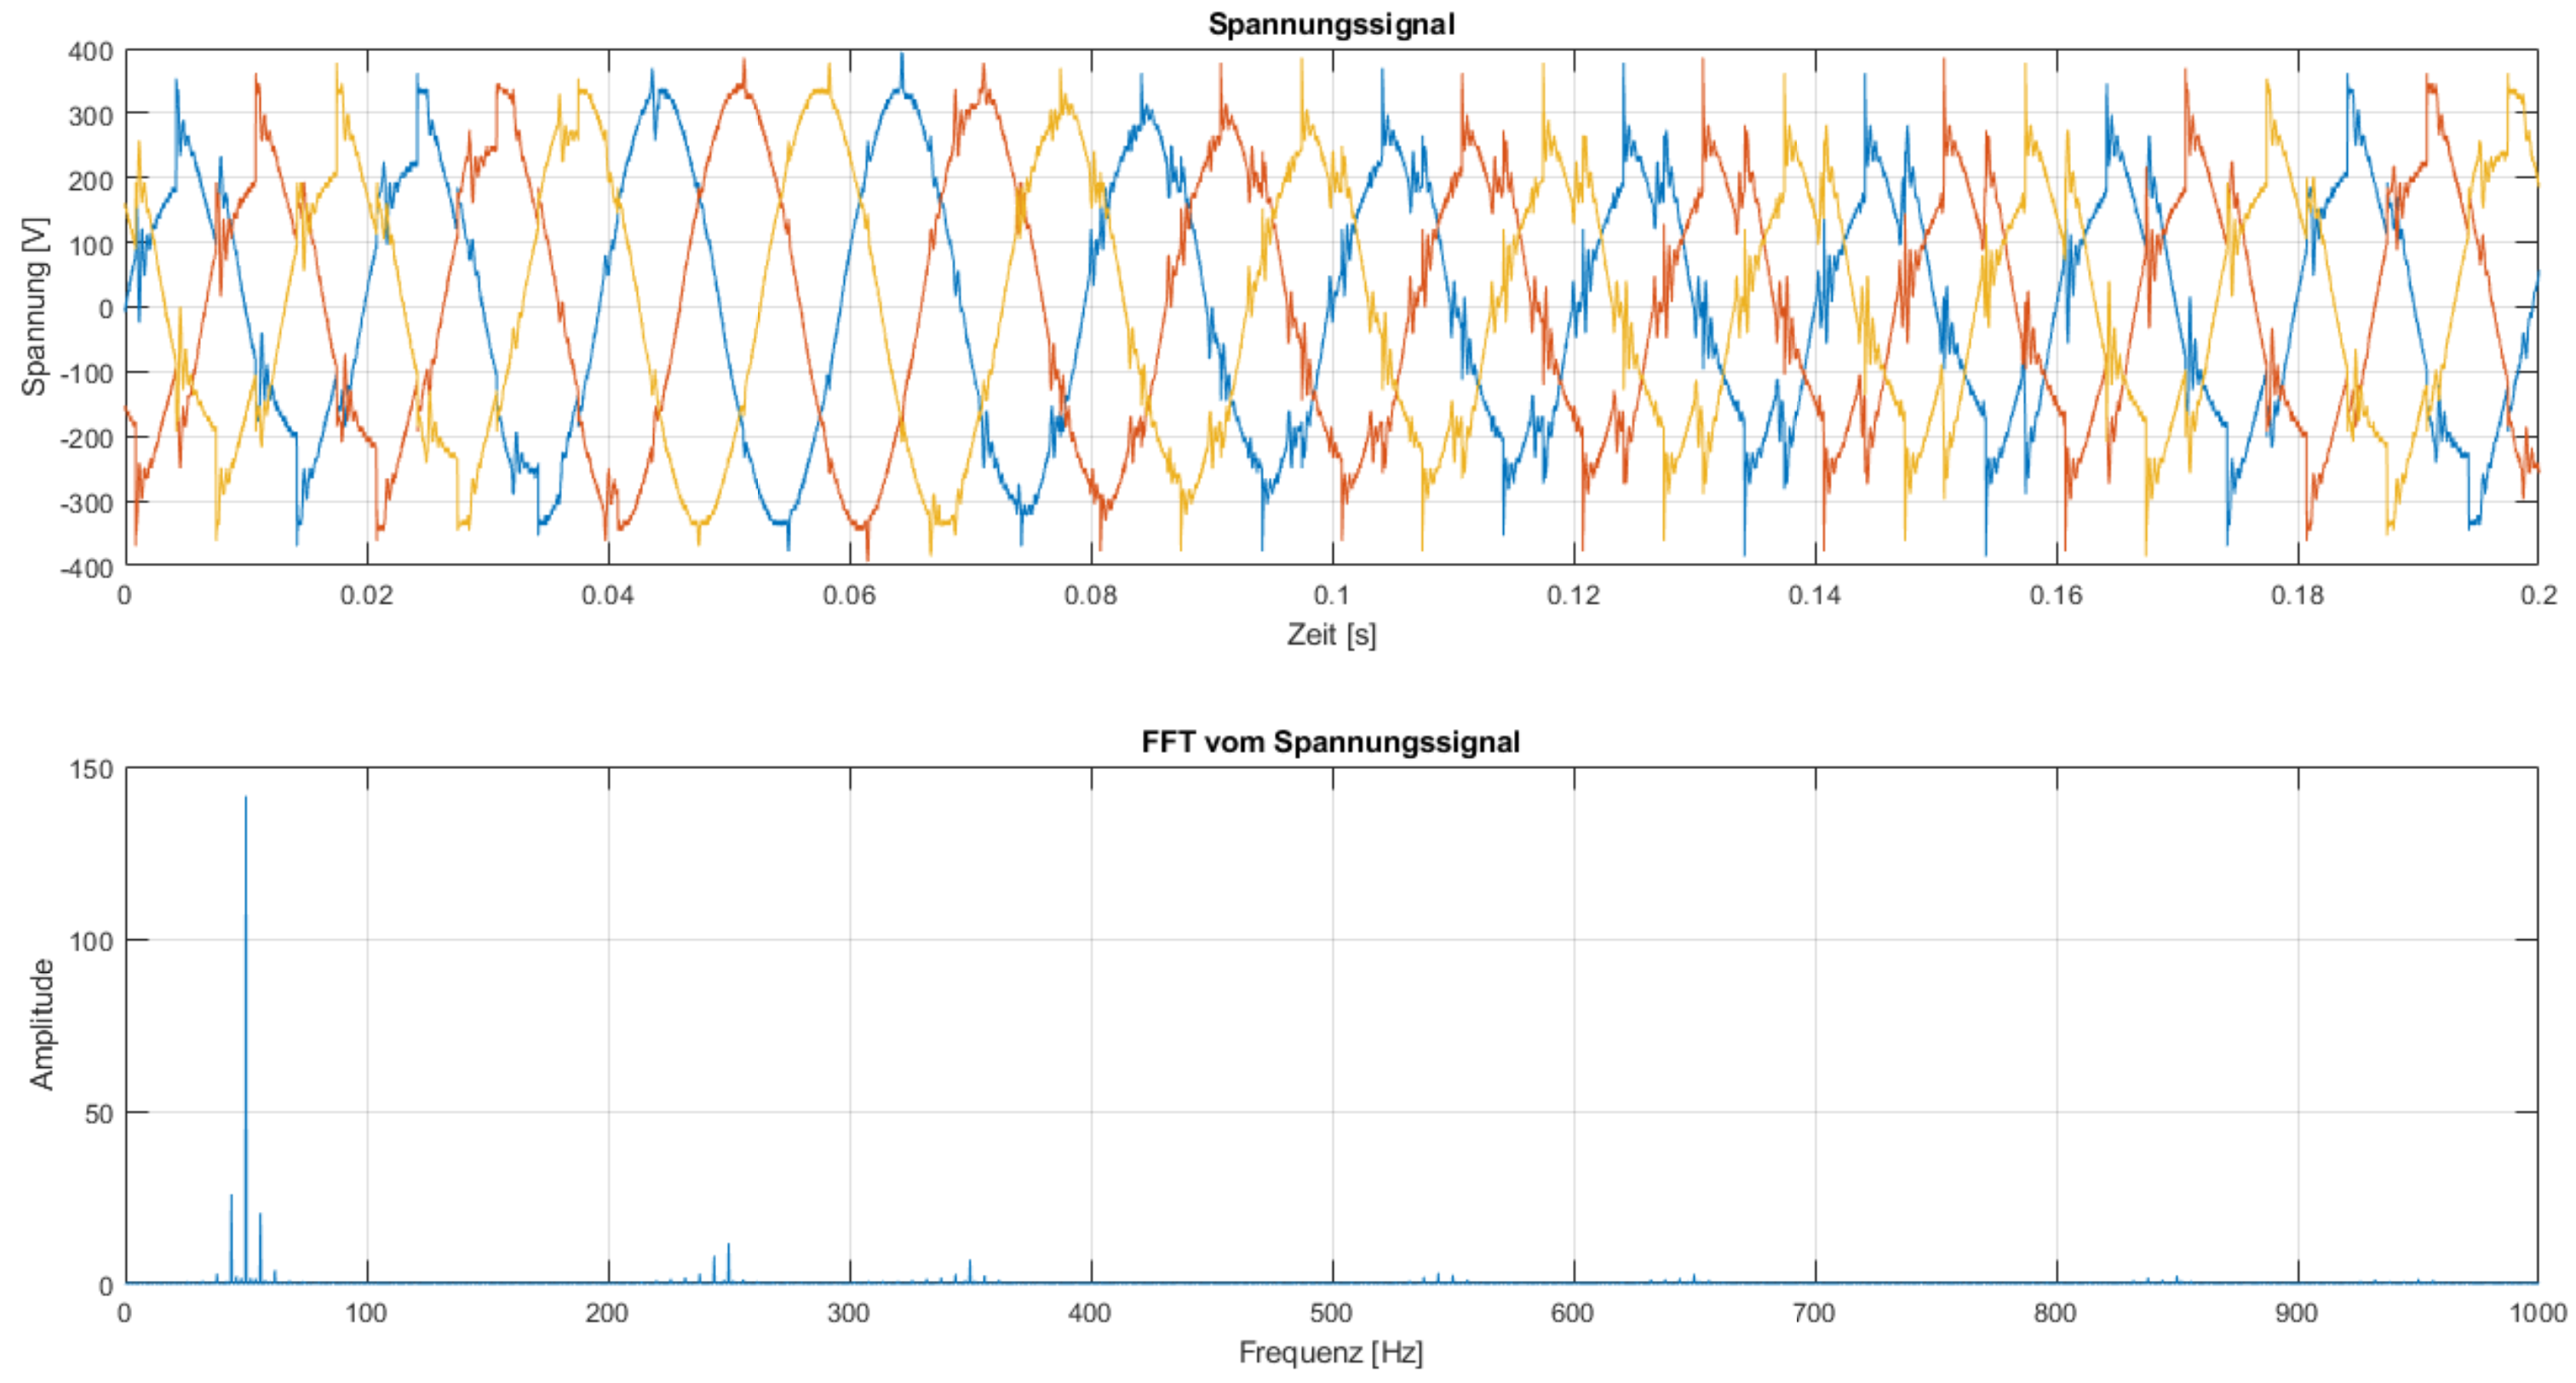
\includegraphics[width=\textwidth]{Messung_ASM_Phas_90grad.png}	
	\caption{Messung mit Phasenanschnitt 90\textdegree}\label{fig:Mess_ASM_Phas90}
\end{figure}

\newpage


\begin{table}[ht!]
	\centering
	\begin{tabular}{|l|l|l|}
		\hline
		Frequenz {[}Hz{]} & Amplitude {[}V{]} & Verhältnis zur Grundschwingung \\ \hline
		44                & 25.896            & 18.31\%                        \\ \hline
		50                & 141.3976          & 100\%                          \\ \hline
		56                & 20.4508           & 14.46\%                        \\ \hline
		244               & 7.9778            & 5.64\%                         \\ \hline
		250               & 11.6537           & 8.24\%                         \\ \hline
		256               & 1.1655            & 0.82\%                         \\ \hline
		344               & 2.7272            & 1.93\%                         \\ \hline
		350               & 6.8988            & 4.88\%                         \\ \hline
		356               & 2.3509            & 1.66\%                         \\ \hline
	\end{tabular}
\caption{Amplitudenwerte bei der Frequenzen bei Phasenanschnitt 90\textdegree}\label{tab:Mess_Spannung_ASM_Phas90}
\end{table}

Anders als beim Phasenanschnitt mit 60\textdegree, beginnt der Asynchronmotor bei einem Winkel von 90\textdegree \hspace{0.02cm} zu schwingen. Dieses Schwingen ist in der Abbildung \ref{fig:Mess_ASM_Phas90} beim Spannungsverlauf ersichtlich. Wird das FFT betrachtet, sind sub- und zwischenharmonische, sowie harmonische Oberwellen erkennbar. Die Amplitudenwerte und das Verhältnis zur Grundschwingung sind für die 1., 5. und 7. Harmonische, sowie deren Seitenbänder sind in der Tabelle \ref{tab:Mess_Spannung_ASM_Phas90} aufgelistet. Betrachtet man die Verhältnisse der Harmonischen Oberwellen, sind die deutlich über den Werten der vorgeschriebenen Normen \ref{sec:Spannungsnormen}. Somit kann der Asynchronmotor nicht mit diesem Verfahren betrieben werden.  


\newpage
\subsubsection*{Sanftes Auf- und Absteuern}

Die Abbildung \ref{fig:Mess_ASM_Sanft_langsam} zeigt ein sanftes Auf- und Absteuern der Spannung.

\begin{figure}[ht!]
	\centering
	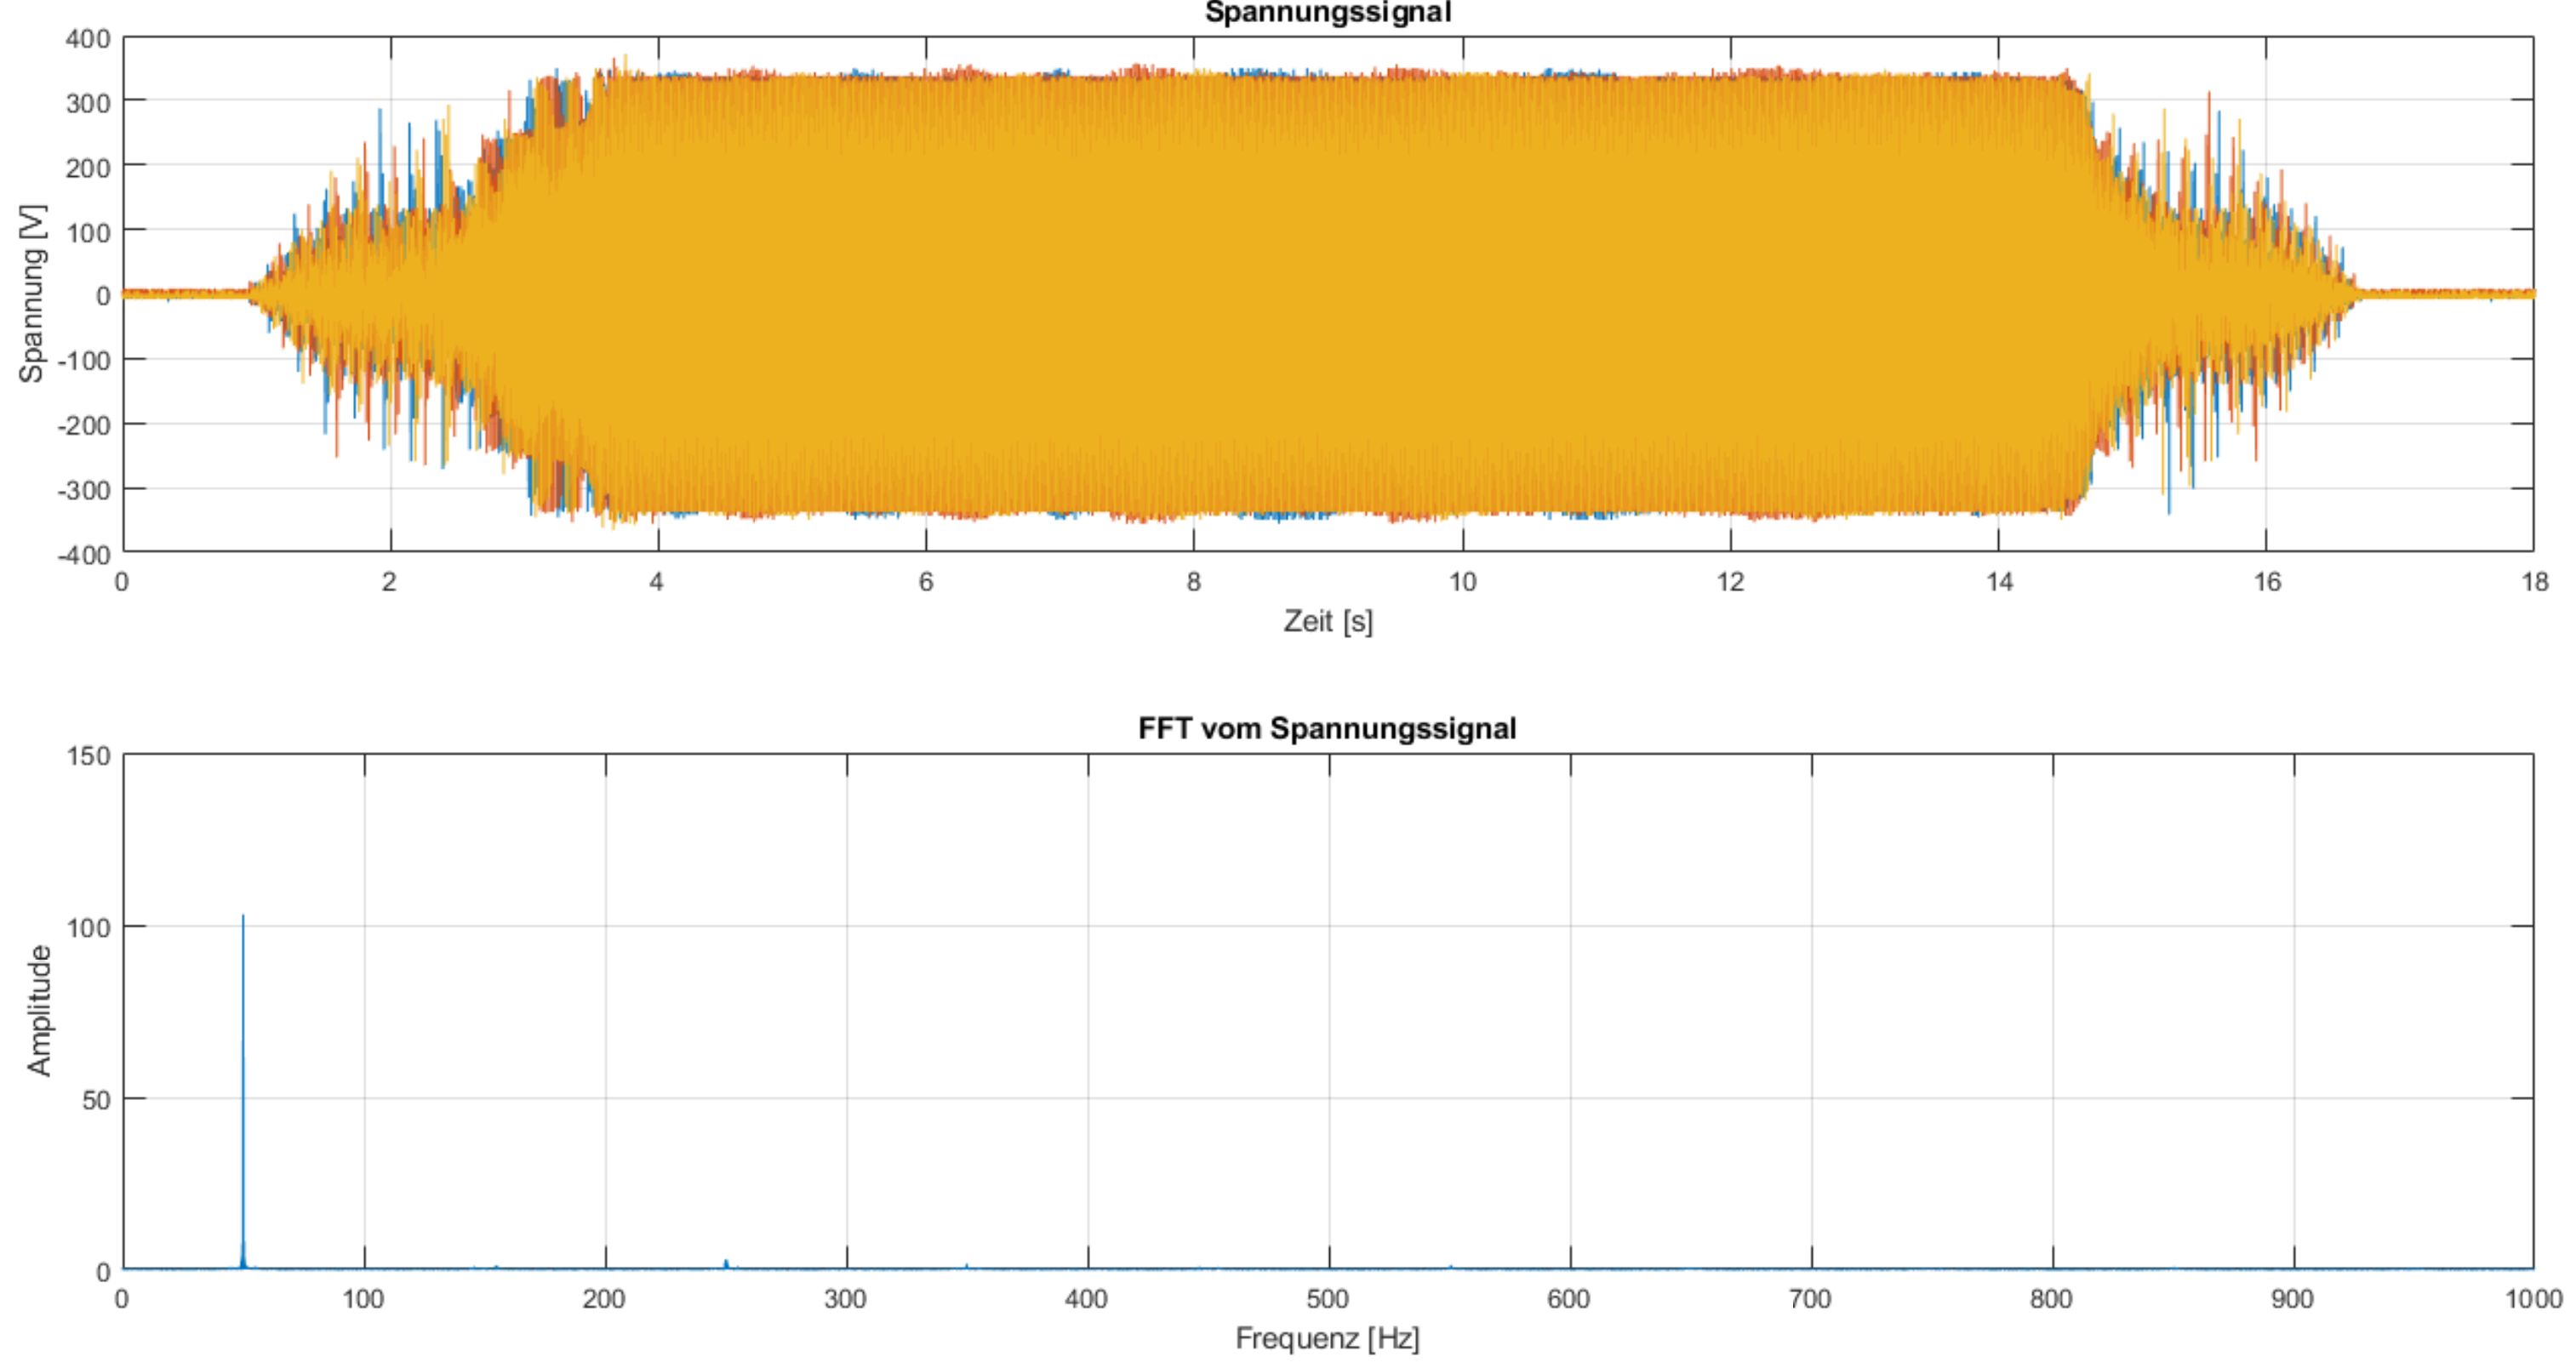
\includegraphics[width=\textwidth]{Messung_ASM_Sanft_langsam.png}	
	\caption{Messung mit sanftem Auf- und Absteuern}\label{fig:Mess_ASM_Sanft_langsam}
\end{figure}


\begin{table}[ht!]
	\centering
	\begin{tabular}{|l|l|l|}
		\hline
		Frequenz {[}Hz{]} & Amplitude {[}V{]} & Verhältnis zur Grundschwingung \\ \hline
		49.85             & 17.3653           & 16.85\%                        \\ \hline
		49.95             & 70.316            & 68.23\%                        \\ \hline
		50                & 103.0639          & 100\%                          \\ \hline
		50.05             & 40.167            & 38.97\%                        \\ \hline
		50.1              & 20.209            & 19.61\%                        \\ \hline
		249.95            & 2.607             & 2.53\%                         \\ \hline
		250               & 1.689             & 1.64\%                         \\ \hline
		250.05            & 2.5084            & 2.43\%                         \\ \hline
	\end{tabular}
\caption{Amplitudenwerte bei der Frequenzen bei sanftem Auf- und Absteuern}\label{tab:Mess_Spannung_ASM_AufAb_sanft}
\end{table}


Bei diesem Steuerungsverfahren sind die harmonischen Schwingungen mit den dazu gehörigen Seitenbänder nur noch minimal erkennbar. Die Resultate der Amplitudenwerte und das Verhältnis zur Grundschwingung befinden sich in der Tabelle \ref{tab:Mess_Spannung_ASM_AufAb_sanft}. Die meisten zwischenharmonischen Schwingungen treten um bei der Grundfrequenz von \SI{50}{Hz} auf. Es ist eine Ähnlichkeit der Seitenbänder zum Verfahren mit dem Widerstand ersichtlich. Vergleicht man die Werte der harmonischen Schwingungen mit den Normen \ref{sec:Spannungsnormen}, befinden diese sich unter den Grenzwerten.



\newpage
\subsection{Sparvariante}
Wie im Kapitel \ref{Spar-Ansteuerung} beschrieben, werden bei der Sparvariante nur ein oder zwei Thyristoren angesteuert. Das Spannungs- und Stromsignal sollen dabei etwa die gleiche Form besitzen wie bei der dreiphasigen Ansteuerung. Da dies bei der Ansteuerung mit einem Thyristor nicht der Fall ist, sind die Messresultate bei diesem Verfahren nicht aufgeführt. Für die Sparvarianten wurden die Verfahren des sanften und harten Auf- und Absteuern betrachtet, da hauptsächlich diese von Interesse sind. Bei den Messung erkennt man, dass die harmonischen Oberwellen der Spannung des Asynchronmotors nicht mit den Normen übereinstimmten. Das gleiche Verhalten wurde bei der ohmschen Last mit harter Ansteuerung bemerkt. Daher wird nur noch das sanfte Hoch- und Runterfahren beim Widerstand analysiert. Alle anderen Messungen die nicht den Normen entsprechen, sind im Anhang im Kapitel \ref{sec:Sparvariante_2Thyristoren} ersichtlich. Die Abbildungen \ref{fig:Mess_2Thyristoren_Widerstand_AufAbFahren_langsam_stroeme} und \ref{fig:Mess_2Thyristoren_Widerstand_AufAbFahren_langsam} sind so aufgebaut, dass zuerst das Spannungs- oder Stromsignal ersichtlich ist. Anschliessend werden die FFT der drei Phasen berechnet und dargestellt. Da es sich um eine unsymmetrische Belastung handelt, wurden alle Phasen separat mit den Normen \ref{sec:Normen} verglichen.

\subsubsection{Strommessung Sparvariante mit einem Widerstand und zwei Thyristoren}

In der Abbildung \ref{fig:Mess_2Thyristoren_Widerstand_AufAbFahren_langsam_stroeme} erkennt man ein sanftes Hoch- und Herunterfahren des Stromes, gemessen durch den Widerstand.

\begin{figure}[ht]
	\centering
	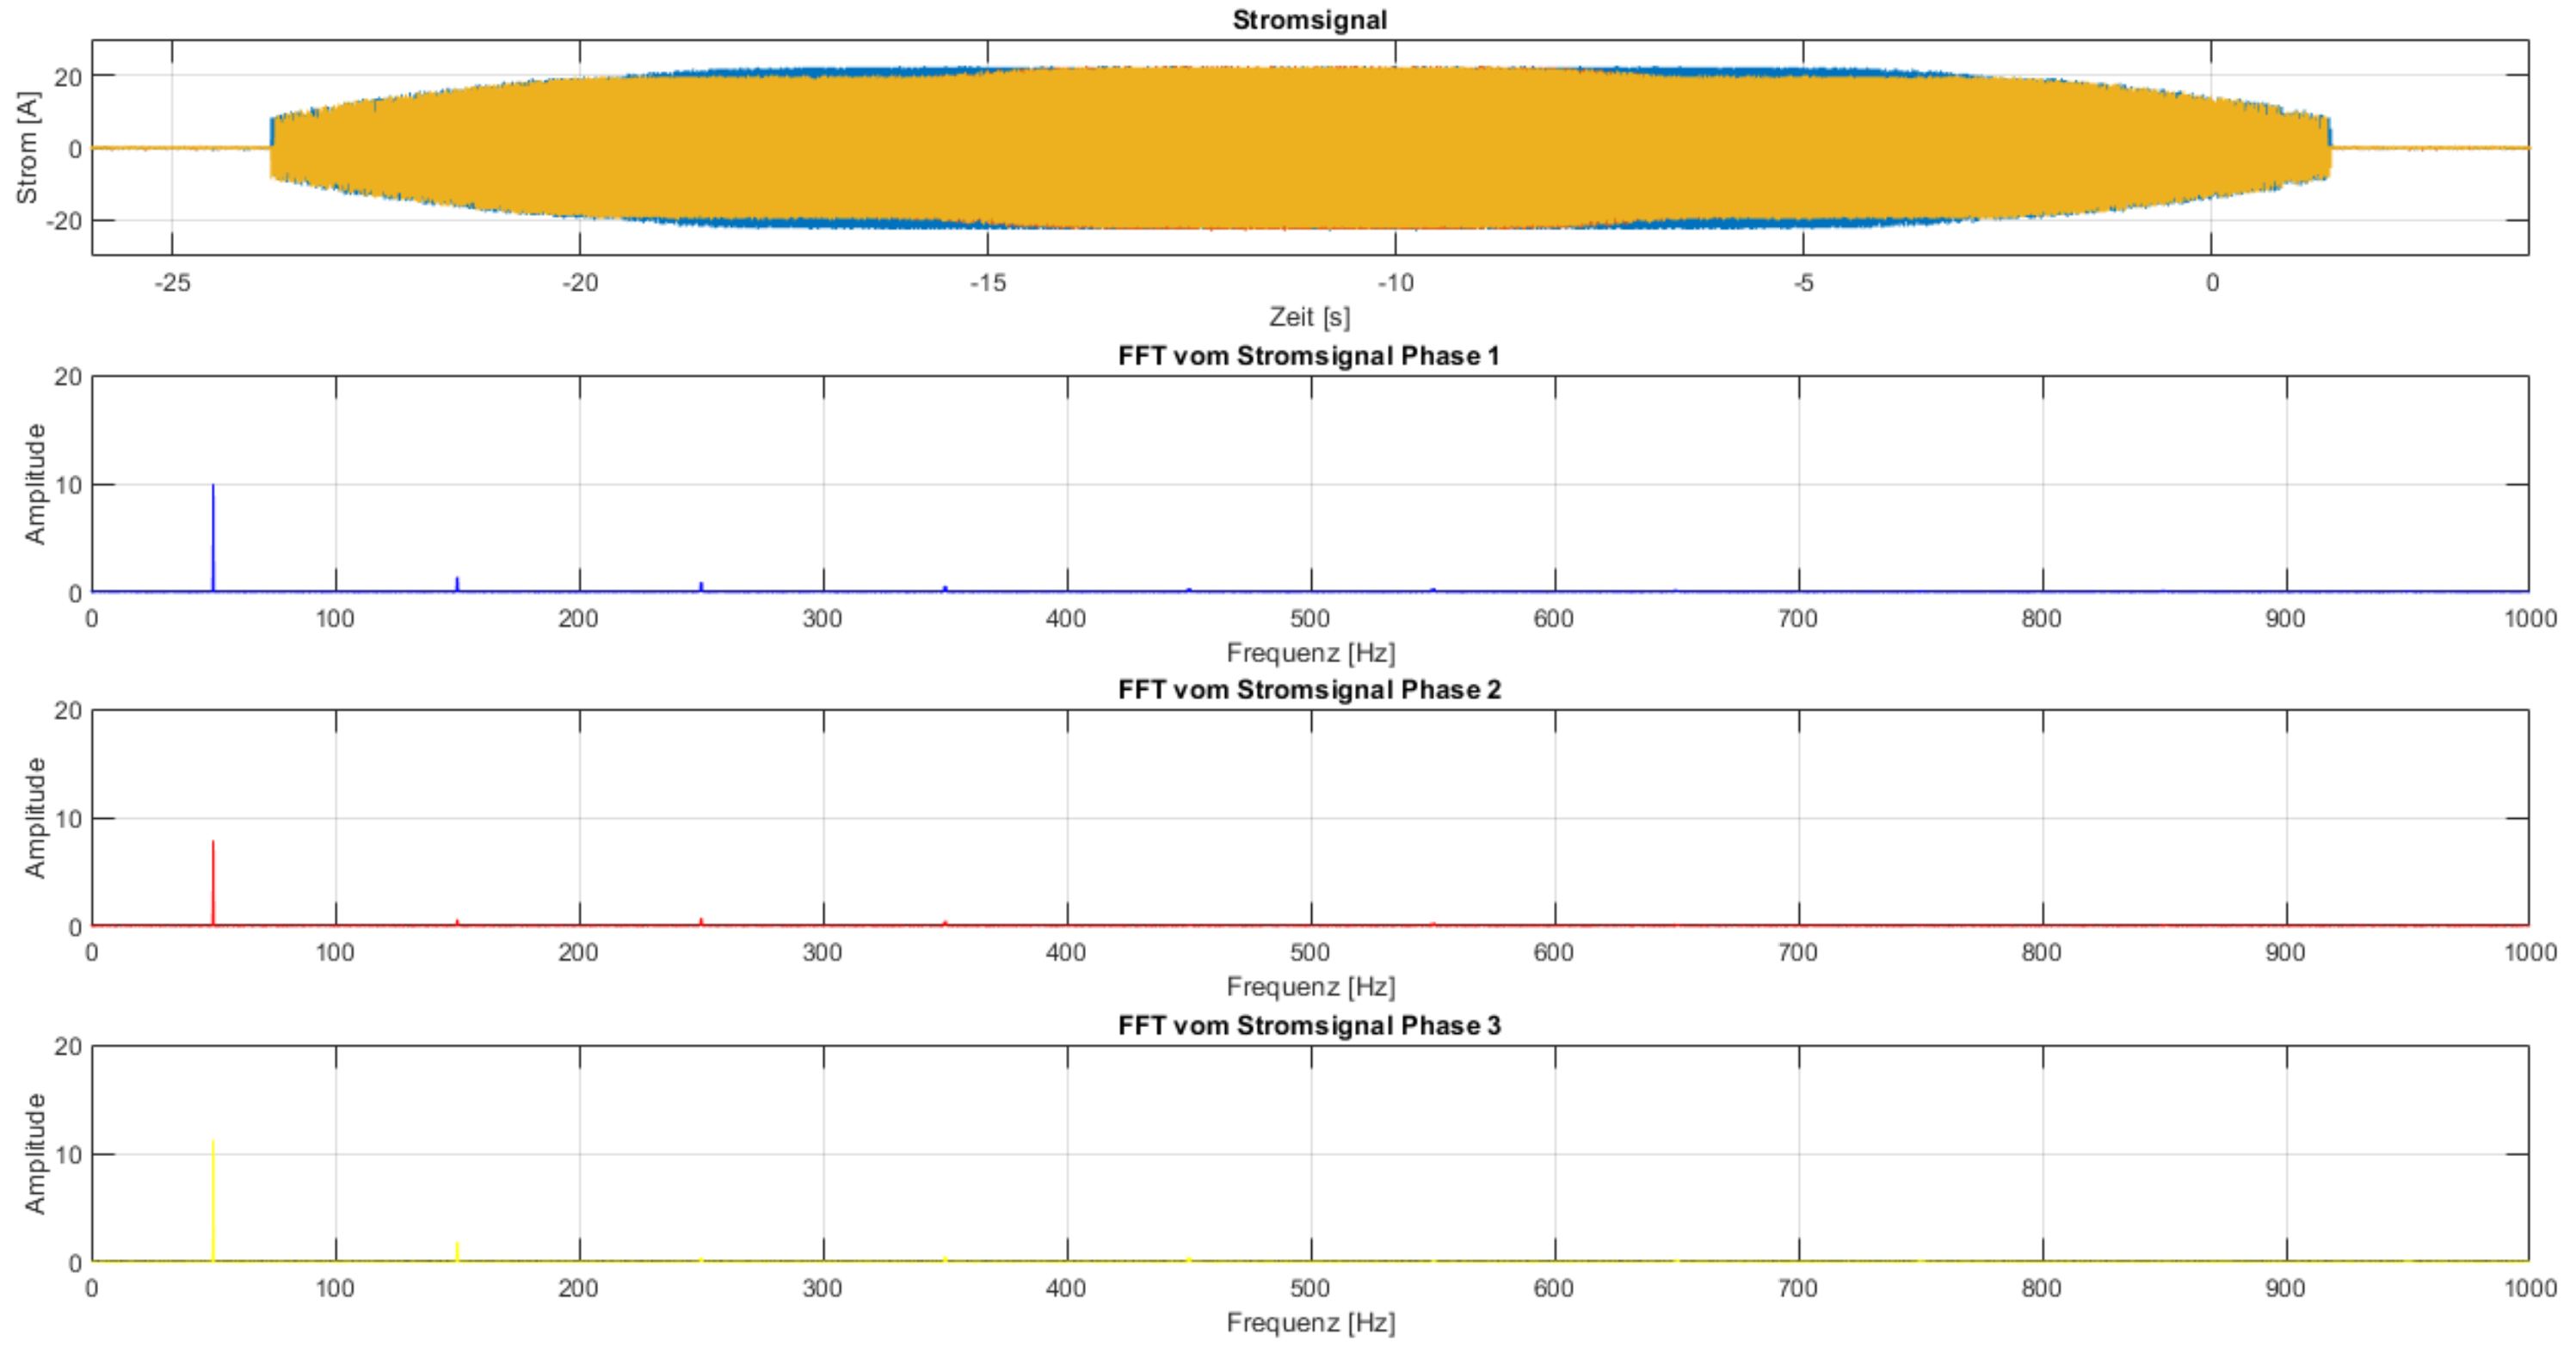
\includegraphics[width=\textwidth]{Messung_Widerstand_2Thyristoren_Stroeme.png}	
	\caption{Strommessung mit dem sanften Auf- und Absteuern und zwei Thyristoren}\label{fig:Mess_2Thyristoren_Widerstand_AufAbFahren_langsam_stroeme}	
\end{figure}

\begin{table}[ht]
	\centering
	\begin{tabular}{|l|l|l|l|}
		\hline
		Frequenz {[}Hz{]} & Amplitude Phase 1 {[}A{]}                                                           & Amplitude Phase 2 {[}A{]}                                                           & Amplitude Phase 3 {[}A{]}                                                           \\ \hline
		49.9              & 4.887                                                                               & 3.749                                                                               & 2.354                                                                               \\ \hline
		49.95             & 9.018                                                                               & 7.485                                                                               & 9.618                                                                               \\ \hline
		50                & 9.951                                                                               & 7.881                                                                               & 11.225                                                                              \\ \hline
		50.05             & 5.193                                                                               & 4.31                                                                                & 3.031                                                                               \\ \hline
		50.1              & 3.057                                                                               & 1.522                                                                               & 1.809                                                                               \\ \hline
		149.93            & 1.381                                                                               & 0.525                                                                               & 1.838                                                                               \\ \hline
		150               & 0.899                                                                               & 0.552                                                                               & 1.103                                                                               \\ \hline
		150.2             & 1.386                                                                               & 0.544                                                                               & 1.829                                                                               \\ \hline
		250		          & 0.372                                                                               & 0.273                                                                               & 0.291                                                                               \\ \hline \hline
		Frequenz {[}Hz{]} & \begin{tabular}[c]{@{}l@{}}Verhältnis zur \\ Grundschwingung\\ Phase 1\end{tabular} & \begin{tabular}[c]{@{}l@{}}Verhältnis zur \\ Grundschwingung\\ Phase 2\end{tabular} & \begin{tabular}[c]{@{}l@{}}Verhältnis zur \\ Grundschwingung\\ Phase 3\end{tabular} \\ \hline
		49.9              & 49.11\%                                                                             & 47.57\%                                                                             & 20.97\%                                                                             \\ \hline
		49.95             & 90.62\%                                                                             & 94.98\%                                                                             & 85.68\%                                                                             \\ \hline
		50                & 100\%                                                                               & 100\%                                                                               & 100\%                                                                               \\ \hline
		50.05             & 52.19\%                                                                             & 54.69\%                                                                             & 27\%                                                                                \\ \hline
		50.1              & 30.72\%                                                                             & 19.32\%                                                                             & 16.12\%                                                                             \\ \hline
		149.95            & 13.88\%                                                                             & 6.66\%                                                                              & 16.37\%                                                                             \\ \hline
		150               & 9.03\%                                                                              & 7\%                                                                                 & 9.83\%                                                                              \\ \hline
		150.05            & 13.93\%                                                                             & 6.9\%                                                                               & 16.29\%                                                                             \\ \hline
		250		          & 3.74\%                                                                             & 3.46\%                                                                               & 2.59\%                                                                             \\ \hline
	\end{tabular}
	\caption{Amplitudenwerte bei der Strommessung mit zwei Thyristoren bei sanftem Auf- und Absteuern}\label{tab:Mess_2Thyristoren_Spannung_Widerstand_AufAb_sanft_stroeme}
\end{table}

Damit die Oberschwingungsströme mit den  Grenzwerten der Normen \ref{sec:Stromnormen} verglichen werden kann, wurde der Effektivwert des Stromes auf die \SI{16}{A} hochgerechnet. Betrachtet man die verschiedenen FFTs der Phasen sind unterschiedliche Peak-Werte zu erkennen. Dies kommt zustande, da es sich um eine unsymmetrische Belastung handelt und die Phase 3 als Rückleiter fungiert. In der Tabelle \ref{tab:Mess_2Thyristoren_Spannung_Widerstand_AufAb_sanft_stroeme} werden die Werte der Amplituden bei verschiedenen Frequenzen und das Verhältnis zur Grundschwingung aufgelistet. Vergleicht man die Werte der 3. und 5. Harmonischen mit den Normen \ref{sec:Stromnormen}, so halten sie die Grenzwerte bei allen drei Phasen ein. Die anderen harmonischen Schwingungen, die nicht in der Tabelle sind, halten die Normen ebenfalls ein.

\newpage
\subsubsection{Spannungsmessung Sparvariante mit einem Widerstand und zwei Thyristoren}

Die Abbildung \ref{fig:Mess_2Thyristoren_Widerstand_AufAbFahren_langsam} zeigt das Spannungssignal über dem Widerstand. 

\begin{figure}[ht!]
	\centering
	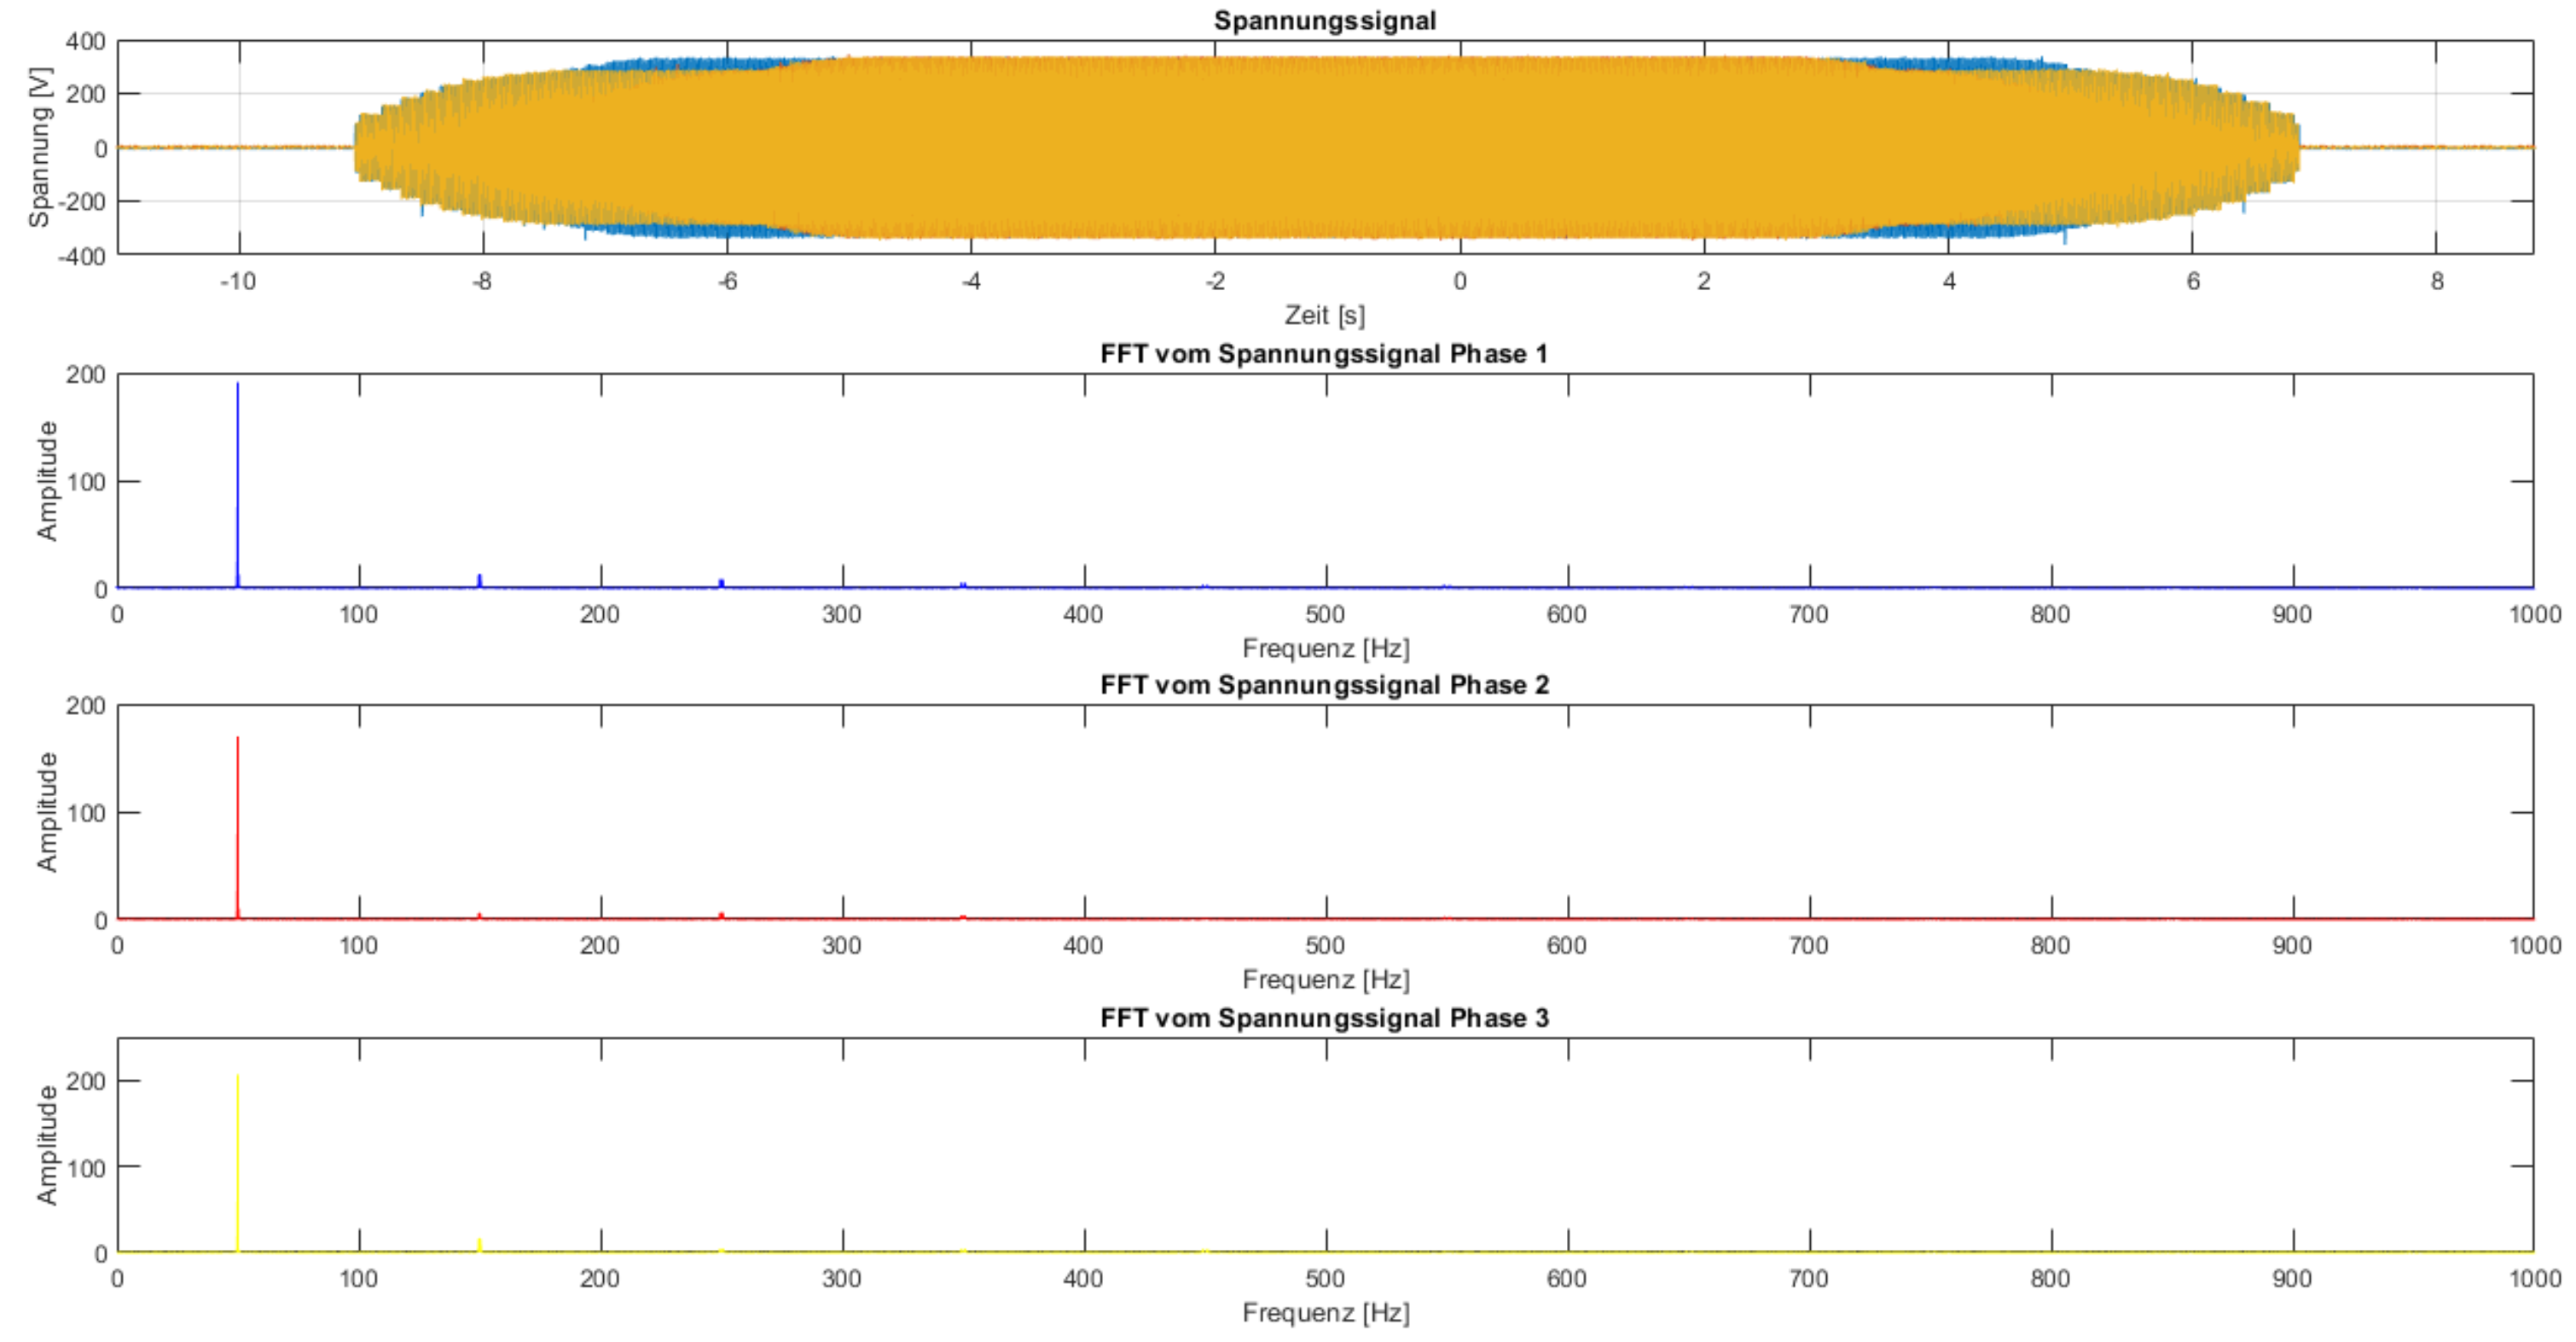
\includegraphics[width=\textwidth]{Mess_2Thyristoren_Widerstand_AufAbFahren_langsam.png}	
	\caption{Messung mit dem sanften Auf- und Absteuern und zwei Thyristoren}\label{fig:Mess_2Thyristoren_Widerstand_AufAbFahren_langsam}	
\end{figure}

Die Spannungsverläufe auf der Abbildung \ref{fig:Mess_2Thyristoren_Widerstand_AufAbFahren_langsam} sehen visuell ähnlich aus wie das sanfte Auf- und Absteuern mit drei Thyristoren, ersichtlich in der Abbildung \ref{fig:Mess_Sanft_langsam}.  Der einziger Unterschied ist, das beim Hoch- und Runterfahren die drei Phasen nicht alle gleich hoch sind. Dies resultiert in einem FFT mit unterschiedlichen Amplitudenhöhen für die verschiedenen Phasen. Die Werte des FFTs sind in der Tabelle \ref{tab:Mess_2Thyristoren_Spannung_ASM_AufAb_sanft} aufgelistet. \\\\

\begin{table}[ht!]
	\centering
	\begin{tabular}{|l|l|l|l|}
		\hline
		Frequenz {[}Hz{]} & Amplitude Phase 1 {[}V{]}                                                           & Amplitude Phase 2 {[}V{]}                                                           & Amplitude Phase 3 {[}V{]}                                                           \\ \hline
		49.9              & 38.5998                                                                             & 19.6499                                                                             & 34.7131                                                                             \\ \hline
		49.95             & 77.5993                                                                             & 82.1127                                                                             & 60.2946                                                                             \\ \hline
		50                & 191.1857                                                                            & 169.7545                                                                            & 206.7036                                                                            \\ \hline
		50.05             & 125.8716                                                                            & 123.6057                                                                            & 126.0935                                                                            \\ \hline
		50.1              & 42.6127                                                                             & 17.4015                                                                             & 26.3464                                                                             \\ \hline
		149.8             & 12.7189                                                                             & 3.9393                                                                              & 16.14                                                                               \\ \hline
		150               & 2.6765                                                                              & 4.3294                                                                              & 5.5055                                                                              \\ \hline
		150.2             & 9.6611                                                                              & 5.9313                                                                              & 13.152                                                                              \\ \hline
		250             & 2.05                                                                              & 0.641                                                                              & 2.334                                                                              \\ \hline \hline
		Frequenz {[}Hz{]} & \begin{tabular}[c]{@{}l@{}}Verhältnis zur \\ Grundschwingung\\ Phase 1\end{tabular} & \begin{tabular}[c]{@{}l@{}}Verhältnis zur \\ Grundschwingung\\ Phase 2\end{tabular} & \begin{tabular}[c]{@{}l@{}}Verhältnis zur \\ Grundschwingung\\ Phase 3\end{tabular} \\ \hline
		49.9              & 20.19\%                                                                             & 11.58\%                                                                             & 16.79\%                                                                             \\ \hline
		49.95             & 40.59\%                                                                             & 48.37\%                                                                             & 29.17\%                                                                             \\ \hline
		50                & 100\%                                                                               & 100\%                                                                               & 100\%                                                                               \\ \hline
		50.05             & 65.84\%                                                                             & 72.81\%                                                                             & 61\%                                                                                \\ \hline
		50.1              & 22.29\%                                                                             & 10.25\%                                                                             & 12.75\%                                                                             \\ \hline
		149.8             & 6.65\%                                                                              & 2.32\%                                                                              & 7.81\%                                                                              \\ \hline
		150               & 1.4\%                                                                               & 2.55\%                                                                              & 2.66\%                                                                              \\ \hline
		150.2             & 5.05\%                                                                              & 3.49\%                                                                              & 6.36\%                                                                              \\ \hline
		250             & 1.07\%                                                                              & 0.38\%                                                                              & 1.13\%                                                                              \\ \hline
		
	\end{tabular}
\caption{Amplitudenwerte bei der Frequenzen mit zwei Thyristoren bei sanftem Auf- und Absteuern}\label{tab:Mess_2Thyristoren_Spannung_Widerstand_AufAb_sanft}
\end{table}

Das Spannungssignal, welches mit nur zwei Thyristoren angesteuert wurde, hat eine visuelle Ähnlichkeit mit dem sanften Auf- und Absteuern der drei Thyristoren \ref{fig:Mess_Sanft_langsam}. Der einzige Unterschied entsteht beim Hoch- und Runterfahren. Die drei Phasen erreichen wegen der unsymmetrischen Belastung nicht die gleiche Höhe. Dies ist bei den FFT ebenfalls ersichtlich. Es sind unterschiedliche Amplitudenhöhen aufgezeigt. Die Werte der FFTs sind in der Tabelle \ref{tab:Mess_2Thyristoren_Spannung_ASM_AufAb_sanft} aufgelistet. Vergleicht man wiederum die Werte der Harmonischen Schwingungen mit den Grenzwerten der Normen, erfüllen sie jedoch den einzuhaltenden Bereich.


\newpage
\subsection{Leistungsfaktor}
Um den Leistungsfaktor für den Phasenanschnitt berechnen zu können, wird die Formeln im Kapitel \ref{sec:Leistungsfaktor} verwendet. Jedoch funktioniert diese Formeln bei der Kombination der verschiedenen Verfahren oder dem Hochfahren durch den Phasenanschnitt nicht. Mit folgender Formel kann der Leistungsfaktor ebenfalls berechnet werden:
\begin{equation}
\lambda = \frac{P}{S}
\end{equation}
Um die Wirkleistung zu erhalten, können die Strom- und Spannungswerte multipliziert werden:
\begin{equation}
P = u(t) \cdot i(t)
\end{equation}
Für die Scheinleistung müssen die Effektivwerte der Spannung und des Stromes multipliziert werden:
\begin{equation}
S = U_{rms} \cdot I_{rms}
\end{equation}
Wobei der Effektivwert des Stromes und der Spannung über die gesamte Zeitdauer berechnet wurde. Der Matlabcode dieser Berechnungen befindet sich im Anhang im Kapitel \ref{sec:Leistungsfaktor_Messungen}. 

Die Resultate der Leistungsfaktorberechnungen sind in der Tabelle \ref{tab:Leistungsfaktor_ASM_Widerstand} aufgeführt.

\begin{table}[ht!]
	\centering
	\begin{tabular}{|l|l|}
		\hline
		Ansteuerungsart ASM                                   		& Leistungsfaktor \\ \hline 
		Sanftes Auf- und Absteuern                          		& 0.2947          \\ \hline
		Sanftes Auf- und Absteuern mit 150$\Omega$ Vorwiderstand 	& 0.3493          \\ \hline
		Phasenanschnitt 90\textdegree                               & 0.4879          \\ \hline
		Phasenanschnitt 60\textdegree                               & 0.4155          \\ \hline \hline
		Ansteuerungsart Widerstand                            		& Leistungsfaktor \\ \hline 
		Sanftes Auf- und Absteuern                          		& 0.9987          \\ \hline
		Hartes Auf- und Absteuern                                   & 0.9988          \\ \hline
		Phasenanschnitt 90\textdegree                         		& 0.9953          \\ \hline
		Phasenanschnitt 60\textdegree                         		& 0.999           \\ \hline
	\end{tabular}
\caption{Leistungsfaktor mit verschiedenen Ansteuerungsverfahren bei der ASM und dem Widerstand}\label{tab:Leistungsfaktor_ASM_Widerstand}
\end{table}
Bei der ASM im Leerlauf gilt, je näher der Leistungsfaktor bei 0 ist desto besser. Da der Leistungsfaktor das Verhältnis von Wirk- zu Scheinleistung ist und sich die Maschine im Leerlauf befindet, wird die Wirkleistung nur für die Ummagnetisierungs- und Eisenverluste benötigt. Wenn der Leistungsfaktor höher ist, heisst dies, dass mehr Verlustleistung entsteht. Um dies zu beweisen wurde ein Vorwiderstand mit \SI{150}{\Omega} in den Stromkreis geschaltet. Dabei konnte festgestellt werden, dass sich wie erwartet mit dem Vorwiderstand der Leistungsfaktor erhöht, da zusätzlich Wirkleistung im Widerstand verheizt wird. Wenn der Leistungsfaktor der verschiedenen Ansteuerungsarten analysiert werden, kann klar gesagt werden, dass sich das sanfte Auf- und  Absteuern am besten eignet für die ASM.

Bei Ohmschen Lasten gilt jedoch, je näher der Leistungsfaktor bei 1 ist, desto besser. Bei den Messungen mit den verschiedenen Ansteuerungsarten wurde festgestellt, dass der Leistungsfaktor beim Phasenanschnitt mit einem Winkel von 60\textdegree \hspace{0.02cm} am höchsten ist. Jedoch verbietet die Normen den Gebrauch des Phasenanschnittes mit den Winkeln von 90\textdegree \hspace{0.02cm} wegen den erhöhten Werten der Amplituden. Deshalb macht es Sinn nur das sanfte und harte Auf- und Abfahren zu vergleichen. Bei diesen zwei Ansteuerungsverfahren hat das harte Auf- und Absteuern einen höheren Leistungsfaktor. Jedoch ist der Unterschied von 0.0001 sehr klein und kann praktisch vernachlässigt werden.
 



%\subsubsection{Schwingungspaketsteuerung mit Last in Stern}
%Für die Messung mit der Schwingungspaketsteuerung wurde eine Einschaltzeit von 0.5 Sekunden und eine Ausschaltzeit von 0.2 Sekunden gewählt. Die Ausschaltzeit darf nicht kürzer sein, da die Spannungsverstärkerschaltung und den Thyristorsteller eine Zeitverzögerung darstellen und so die Spannung nicht sofort ein- oder ausgeschaltet wird. Wenn die Ausschaltzeit kürzer ist, geht die Spannung zwischen den Paketen nicht auf \SI{0}{V}. 
%\begin{figure}[ht!]
%	\centering
%	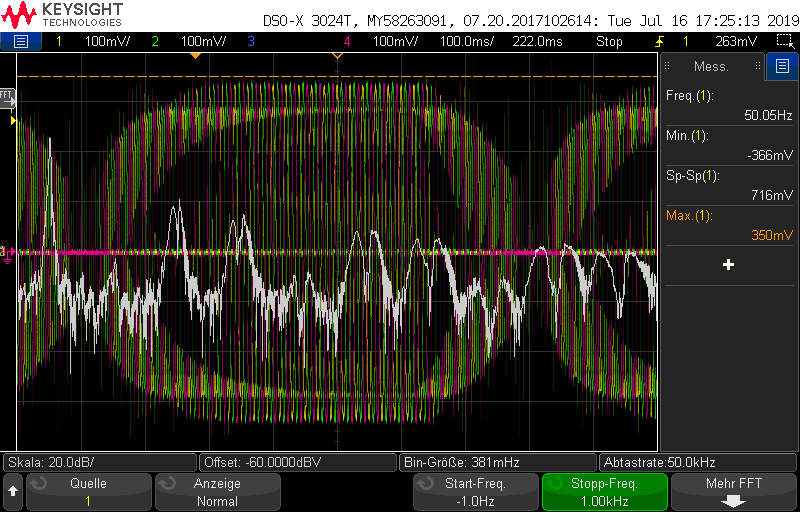
\includegraphics[width=0.7\textwidth]{Schwingungspaket_kurz.png}	
%	\caption{Das Spannungssignal aller Phasen bei Schwingungspaketsteuerung mit FFT}\label{fig:Mess_Schwing_kurz}
%\end{figure}
%
%Das FFT zeigt entgegen den Erwartungen aus der Theorie fast keine Subharmonische auf. Dafür sind Harmonische und Zwischehamrnische sehr ausgeprägt. Sehr gut zu sehen ist die Grundfrequenz von \SI{50}{Hz}, der erste Peak von der linken Seite. Dies ist darauf zurückzuführen, dass nicht direkt ein- und ausgeschaltet wird und so einem Sanft-Anlass ähnelt. Dies dominiert gegenüber dem harten Ein- und Ausschalten, welches die Subharmonische hervorrufen würde.
%\newpage
%\subsection{Phasenanschnittsteuerung mit 2 Thyristoren mit Last in Stern}
%Für die Sparansteuerung wurde ein Winkel von 90\textdegree \hspace{0.02cm} gewählt. 
%
%\begin{figure}[ht!]
%	\centering
%	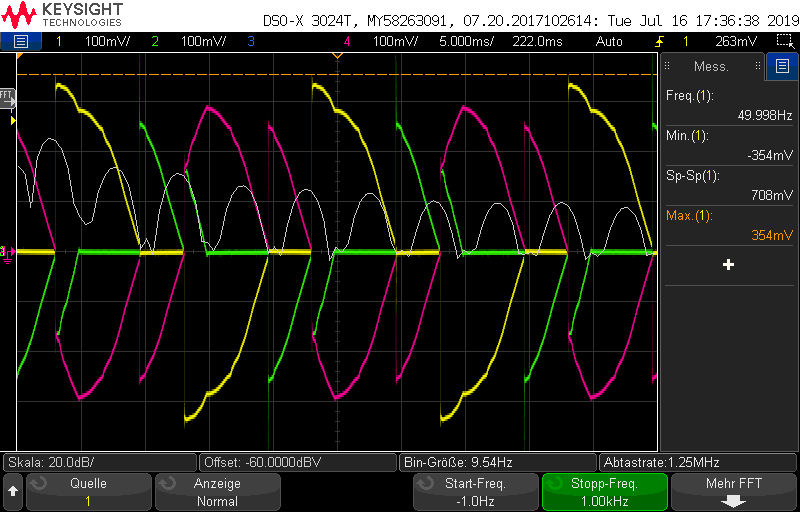
\includegraphics[width=0.7\textwidth]{2phas_90grad_kurz.png}	
%	\caption{Das Spannungssignal aller Phasen bei Schwingungspaketsteuerung mit FFT}\label{fig:Mess_2phas_kurz}
%\end{figure}
%
%
%\subsection{Phasenanschnittsteuerung mit 1 Thyristor mit Last in Stern}
%Für die Sparansteuerung wurde ein Winkel von 90\textdegree gewählt. 
%
%\begin{figure}[ht!]
%	\centering
%	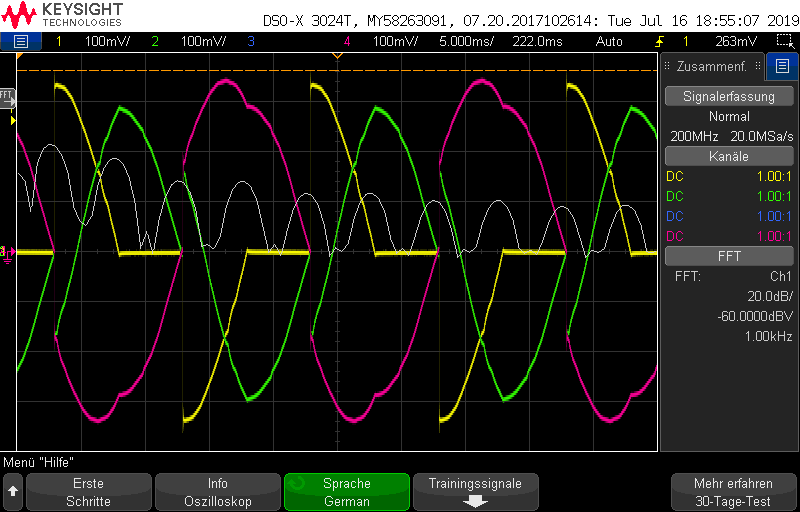
\includegraphics[width=0.7\textwidth]{1phas_90grad_kurz.png}	
%	\caption{Das Spannungssignal aller Phasen bei Schwingungspaketsteuerung mit FFT}\label{fig:Mess_1phas_kurz}
%\end{figure}





\section{Interpretation der Resultate}\label{sec:Interpretation_Resultate}
Bei den Interpretationen der Resultate werden noch einmal die unterschiedliche Messungen und deren Auswertung analysiert und wichtige Schlussfolgerungen dokumentiert. Dabei haben das Einhalten der Normen die oberste Priorität. Wenn eine Ansteuerungsart die Normen bei dem Widerstand nicht einhält, muss dies bei der ASM nicht auch der Fall sein. Des Weiteren wird begründet welche Ansteuerungsarten, bei den verschiedenen Lasten, sinnvoll ist. Schlussendlich wird bei den Messungen der höchst beziehungsweise der niedrigste Leistungsfaktor bestimmt.


\subsection{Resultate der Ansteuerungsarten beim Widerstand}
Für den Widerstand wurden zuerst die Strommessungen der verschiedenen Ansteuerungsarten durchgeführt. Die Resultate der FFTs konnten unmittelbar mit den Grenzwerten der Oberschwingungsströme \ref{sec:Stromnormen} verglichen werden. Dabei wurden, die Ströme auf den maximalen Effektivstrom von \SI{16}{A} hoch gerechnet. Dazu wurde der höchste Spitzenwert der Messdaten genommen und auf \SI{16}{A} hoch skaliert. Nur so war es möglich die maximalen erlaubten Ströme der Messungen mit den Normen zu vergleichen. Die Phasenanschnittsteuerungen mit den Winkeln von 60\textdegree \hspace{0.02cm} und 90\textdegree \hspace{0.02cm} erfüllten die Normen nicht. Da bei der Oberschwingungsströme nur die Grenzwerte der harmonische Schwingungen aufgelistet sind und diese bei der Schwingungspaketsteuerung nicht auftreten, wurde bei dieser Ansteuerungsart die Ströme nicht gemessen. Das sanfte und harte Auf- und Absteuern hingegen verglich man mit den Normen \ref{sec:Stromnormen}, da bei diesen Ansteuerungsarten harmonische Oberschwingungsströme auftreten. Diese sind jedoch im Verhältnis zur Grundschwingung so klein, dass sie die Grenzwerte einhalten.\\ 

Wenn die Ansteuerungsart die Grenzwerte der Oberschwingungsströme einhalten, wurden die Messwerte der Spannungen mit den Grenzwerten der harmonischen Oberschwingungsspannung, die in der Norm 61000-2-2 \ref{sec:Spannungsnormen} behandelt wurden, verglichen. Dabei sind die 5., 7. und 11. Harmonischen in den Tabellen der Messwerte aufgelistet. Die sonstigen harmonischen Oberschwingungen, bis zur 23. Ordnung, wurden ebenfalls mit der Norm verglichen, jedoch nicht mehr in die jeweiligen Tabellen eingeführt. Dabei erfüllten das sanfte und harte Auf- und Absteuern ebenfalls die Grenzwerte der Oberschwingungsspannung.\\

Die Norm 61000-2-2 enthält ausserdem die Grenzwerte, welche die Spannungen der sub- und zwischenharmonischen Schwingungen einhalten müssen. Sie bezieht sich jedoch nur auf die \SI{230}{V}-Systeme. Deshalb konnten die Messresultate nicht mit dieser Norm verglichen werden. Die Auswirkungenen der sub- und zwischenharmonischen Schwingungen sind im Kapitel \ref{sec:Spannungsnormen} beschrieben. Aus der Tabelle \ref{tab:kompatibilitätsstufen} wurde jedoch erkannt, dass die zugelassenen Grenzwerte welche sich näher bei der Grundschwingung befinden, ein grösser Peak-Wert haben dürfen, als jene die weiter weg von der Grundschwingung sind. So kann argumentiert werden, dass beim sanften und harten Auf- und Absteuern die Seitenbänder um die Grundschwingung näher beieinander sind als bei der Schwingungspaketsteuerung. Welche Auswirkungen der Abstand der Seitenbänder hat, konnte nicht geklärt werden. Es wird vermutet, dass je näher die Bänder an den jeweiligen harmonischen Ordnung sind, desto weniger Störungen werden ins Netz zurück gespeist. Somit würden die sanfte- und harte Ansteuerung einen saubereren Sinus heraus geben als die Schwingungspaketsteuerungen. Vergleicht man die Seitenbänder der erst genannten Verfahren miteinander erkennt man, dass die Frequenzen, bei denen die sub- und zwischenharmoisch Schwingungen auftreten, beim der sanft-Ansteuerung näher beieinander sind.\\

Der THD-Wert der Messungen ist nicht bestimmt worden, da diese Berechnungen nur für den stationären Betrieb konzipiert sind. Da keines der Signale welche die Stromnormen erfüllten stationär sind, wurden diese Berechnungen weggelassen. Der Flickerwert wurde ebenfalls nicht gemessen, da keine geeignete Laboreinrichtung und kein Messgerät vorhanden war.\\

Wenn die Leistungsfaktoren des sanften und harten Auf- und Absteuerns miteinander verglichen werden fällt auf, dass diese fast gleich gross sind. Der kleine Unterschied von 0.0001 kann vernachlässigt werden. Deshalb kann aufgrund des Leistungsfaktors gesagt werden, dass die beiden Ansteuerungsarten gleichwertig sind.\\

Die Sparvariante mit zwei Thyristoren eignet sich nur bedingt für die Ansteuerung einer ohmschen Last. Das harte Auf- und Absteuern erfüllt die Grenzwerte der Oberschwingungsspannung \ref{sec:Spannungsnormen} nicht. Einzig das sanfte Auf- und Absteuern erfüllen die Spannungs- und Stromnorm. Das Problem ist jedoch, dass die Phasen stark unterschiedlich belastet werden. Beim FFT können relative Unterschiede bei den Spannungen von bis zu 10\% und bei den Strömen von bis zu 28\% festgestellt werden.\\

Schlussendlich erkannte man, dass sich das sanfte Auf- und Absteuern am besten eignet um einen Widerstand anzusteuern. Dies Aufgrund der dünnen Seitenbänder bei den harmonischen Oberschwingungen, des hohen Leistungsfaktors und der kleinen Amplitude der auftretenden harmonischen Oberwellen.

\subsection{Resultate der Ansteuerungsarten bei der ASM}
Da im Voraus die Strommessungen vollzogen wurden, welche für ihre jeweilige Last Sinn ergeben, wurden nicht mit allen Ansteuerungsarten die ASM angesteuert. Für die Schwingungspaketsteuerung und das harte Auf- und Abfahren der Leistung ist keine Anwendungen für die Maschine bekannt. Deshalb verzichtete man auf die Messungen dieser Steuerungsarten.\\


Bei der Asynchronmaschine wurden zuerst die Strommessungen der Phasenanschnittsteuerung mit den bekannten Winkeln von 60\textdegree und 90\textdegree \hspace{0.02cm} sowie das sanfte Auf- und Asteuern des Stromes, durchgeführt. Die Werte des Effektivstromes wurde wieder mit einem Faktor auf die \SI{16}{A} hoch skaliert, um den maximalen erlaubten Stromstromwerte zu erhalten. So konnten die Grenzwerte der Oberschwingungsströme mit den dazugehörigen Normen verglichen werden. Anders als bei dem Widerstand, erfüllen alle untersuchten Ansteuerungsarten die Grenzwerte der Normen. Deshalb konnte man in einem zweiten Messverfahren die Oberschwingungsspannungen untersuchen.\\

Bei der ASM handelt es sich wie auch beim Widerstand um ein \SI{400}{V}- und nicht ein \SI{230}{V}-System. Deshalb konnten die sub- und zwischenharmonischen Schwingungen der Messungen nicht mit den Normen verglichen werden.
Da jedoch die Schwingungspaketsteuerung und das harte Auf- und Abfsteuern der ASM nicht verwendet wird, schloss man daraus, dass die Ansteuerungsarten welche kritische Seitenbänder hervorruft, nicht mehr vorhanden sind. 

Das FFT des Phasenanschnitt 60\textdegree \hspace{0.02cm} zeigt bei allen drei Phasen, einen fast perfekten Sinus auf.
Die harmonischen Oberschwingungen im Verhältnis zur Grundschwingung betragen desshalb nur maximal 1.5\%. Sub- und Zwischenharmonische sind ebenfalls kein vorhanden. Dies erkennt man auch nach betrachten des Spannungssignals.
Der Phasenanschnitt mit 90\textdegree \hspace{0.02cm} ist für die Ansteuerung der ASM nicht geeignet, da die harmonischen Oberschwingungen die Grenzwerte der Norm \ref{sec:Spannungsnormen} nicht einhalten. 
Beim sanften Auf- und Absteuern sind harmonische Schwingungen zu erkennen. Sie halten jedoch die Grenzwerte ein. Zudem existieren sub- und zwischenharmonische Schwingungen. Im Vergleich zur Ansteuerung mit dem Phasenanschnitt von 60\textdegree \hspace{0.02cm} sind die Verhältnisse zur Grundschwingung grösser.\\ 

Für den Leistungsfaktor verglich man nur noch das sanfte Auf- und Absteuern mit der Phasenanschnittsteuerung mit einem Winkel von 60\textdegree \hspace{0.02cm}. Bei der ASM gilt, je näher der Leistungsfaktor bei 0 ist, desto niedriger sind die Ummagnetisierungs- und Eisenverluste. Anders als beim Faktor des Widerstandes, gibt es beim Leistungsfaktor der ASM grössere Unterschiede, wobei dieser zwischen dem sanften Auf- und Absteuern und Phasenanschnitt 60\textdegree \hspace{0.02cm} 0.1208 beträgt. Das sanfte Auf- und Abfahren hat einen tieferen Leistungsfaktor als der Phasenanschnitt mit dem Winkel von 60\textdegree. \\

Wie auch bei der Widerstandsmessung wurde bei der ASM eine Sparvariante mit zwei Thyristoren untersucht. Sie haltet jedoch die Grenzwerte der Oberschwingungsströme nicht ein. Die Variante wurde deshalb nicht mehr aufgezeigt.\\

Als Fazit für die verschiedenen Ansteuerungsarten erkannte man, dass sich das sanfte Auf- und Absteuern auch bei der ASM am besten eignet. Zwar zeigte das FFT des Phasenanschnittes mit 60\textdegree \hspace{0.02cm} keine harmonische Oberschwingungen, jedoch waren sie beim sanften Auf- und Absteuern in Rahmen der erlaubten Grenzwerte der Normen. Der Leistungsfaktor des sanften Auf- und Absteuern ist tiefer als der des Phasenanschnittes mit 60\textdegree \hspace{0.02cm} und deshalb besser.

\subsection{Vergleich der Messungen mit den Simulationen}
Für den Vergleich der Messungen mit den Simulationen gab es grosse Abweichung zwischen den verschiedenen Werten der FFTs. Es stellte sich als schwierig heraus bei komplexeren Ansteuerungsarten wie das sanfte und harte Auf- und Absteuern, die gleichen Zeiten für die Steigung und das Halten auf maximaler Spannung zu erreichen. Ein zusätzliches Problem stellte der Thyristorsteller und die Spannungsverstärkung dar, da diese eine Verzögerung besassen. Zusätzlich werden in der Simulation die Bauteile als ideal angenommen wobei dies bei den Messungen nicht der Fall ist. Erste Einblicke in das Simulation-Tool Plecs und das Verständnis des Verhalten von verschiedenen Ansteuerungsarten konnten trotzdem gewonnen werden. 








\section{Schlusswort}
Das Ziel der vorliegenden Bachelorarbeit war es, eine Kombination von zwei geläufigen Ansteuerungsverfahren zu entwickeln, welche störende Oberschwingungen minimiert. Anhand eines Laboraufbaus sollte die gefunden Steuerungen mit den Grenzwerten der Normen geprüft werden.\\ 
Die Ergebnisse der beiden Verfahren, Phasenanschnitt- und Schwingungspaketsteuerung, konnten analytisch auf verlustbehaftete Oberwellen untersucht werden. Dabei wurde erkannt, dass je grösser der Winkel des Phasenanschnittes gewählt wird, desto gösser werden die Amplitudenwerte der harmonischen Oberschwingungen. Bei der Schwingungspaketsteuerung treten, bei kleinerem Duty Cycle, mehr Sub- und Zwischenharmonische auf. Mithilfe der Simulations-Tools, Matlab und Plecs, konnten die einphasige analytische Untersuchung, der beiden Steuerverfahren, ausgeführt und verifiziert werden. Es zeigte sich, dass beide Tools die gleichen Werte des Amplitudenspektrums erhalten haben.\\ 
Der dreiphasige Vergleich mit Plecs und dem Laboraufbau hat gezeigt, dass die Amplitudenspektren Ähnlichkeit miteinander haben. Vergleicht man jedoch die Werte der beiden Spektren, ist vor allem beim sanften und harten Auf- und Absteuern eine grosse Differenz erkennbar. Der Grund dafür ist, dass sich die Steilheit des Auf- und Absteuern beim praktischen Aufbau anders verhält als bei der theoretischen Simulation.\\
Die Kombination der beiden Ansteuerungsverfahren wurde mit Plecs im ein- und dreiphasigen System aufgebaut. Mit dem Arduino und der selber geschriebenen Software, konnte sie beim Laboraufbau implementiert werden. Die Steilheit des Auf- und Absteuern, die Dauer der maximalen Spannung sowie die Anzahl der eingeschalteten Paketen des dreiphasigen Thyristorstellers können manuell im Programm eingestellt werden. Es stellte sich heraus, dass das sanfte Auf- und Absteuern der Leistung das geeignetste Verfahren ist, um die beiden Lasten (Widerstand und Asynchronmaschine) anzusteuern. Die Werte der Oberschwingungsströmen und -spannungen halten die Grenzwerte der Normen ein. Auch der untersuchte Leistungsfaktor hat bei dem Verfahren im Vergleich zu den anderen Ansteuerungsarten den besten Wert erhalten.\\
Beim Aufbau der Sparvarianten, mit Ansteuerung von zwei Thyristoren, wurde erkannt, dass die ASM die Grenzwerte der Oberschwingungsspannung nicht einhaltet. Beim Widerstand erfüllt sie grundsätzlich die Normen, jedoch werden die Phasen unterschiedlich stark belastet. Deshalb sind auch diese Verfahren nicht für die Ansteuerung geeignet.\\
Leider konnten, aus Zeitgründen, keine genaueren Erkenntnisse zu den Netzrückwirkung von sub- und zwischenharmonischen Oberwellen gefunden werden. Sie treten vor allem bei Steuerungsarten mit Schwingungspakete auf. Es wird jedoch vermutet, dass je näher die Seitenbänder an den jeweiligen Harmonischen sind, desto weniger störend sind sie für die elektrischen Geräte.\\
Mithilfe eines selbst gebauten Thyristorstellers wäre es möglich gewesen, alle drei Phasen unterschiedlich anzusteuern. Damit könnte das Verhalten der Halbwellensteuerung im Laboraufbau vollzogen und untersucht werden.\\
Am Ende des Projektes kann durchaus eine positive Bilanz gezogen werden. Auch wenn bei den Verfahren die Auswirkung der sub- und zwischenharmonischen der verschiedenen Ansteuerungsarten nicht herausgefunden wurde. Das Projekt hat gezeigt, dass es möglich ist, mit einer Kombination von zwei Steuerungsverfahren störende Oberschwingungen zu vermeiden. Zudem konnten neue und wichtige Erkenntnisse des Simulationsprogrammes Plecs realisiert werden.  






\section*{Ehrlichkeitserklärung}
Wir erklären eidesstattlich, dass wir die vorliegende Arbeit selbstständig und ohne fremde Hilfe verfasst, andere als die angegebenen Quellen nicht benutzt und die benutzten Quellen entnommenen Stellen als solche gekennzeichnet haben. Die Arbeit wurde bisher in gleicher oder ähnlicher Form keiner anderen Prüfungsbehörde vorgelegt.\\\\

Nando Spiegel \hspace{8cm} Bastian van Dijke\vspace{2cm}\\\\
------------------------------- \hspace{6.45cm} -------------------------------\\\\



Windisch, am 16.08.2019 



%%---BIBLIOGRAPHY------------------------------------------------------------------------
{\sloppypar
\printbibliography[heading=bibintoc]
\label{sec:lit}
}
\listoffigures
\listoftables
%%---APPENDIX----------------------------------------------------------------------------
\begin{appendix} %Anhang
\section{Projektvereinbarung}	
\begin{figure}[ht!]
	\centering
	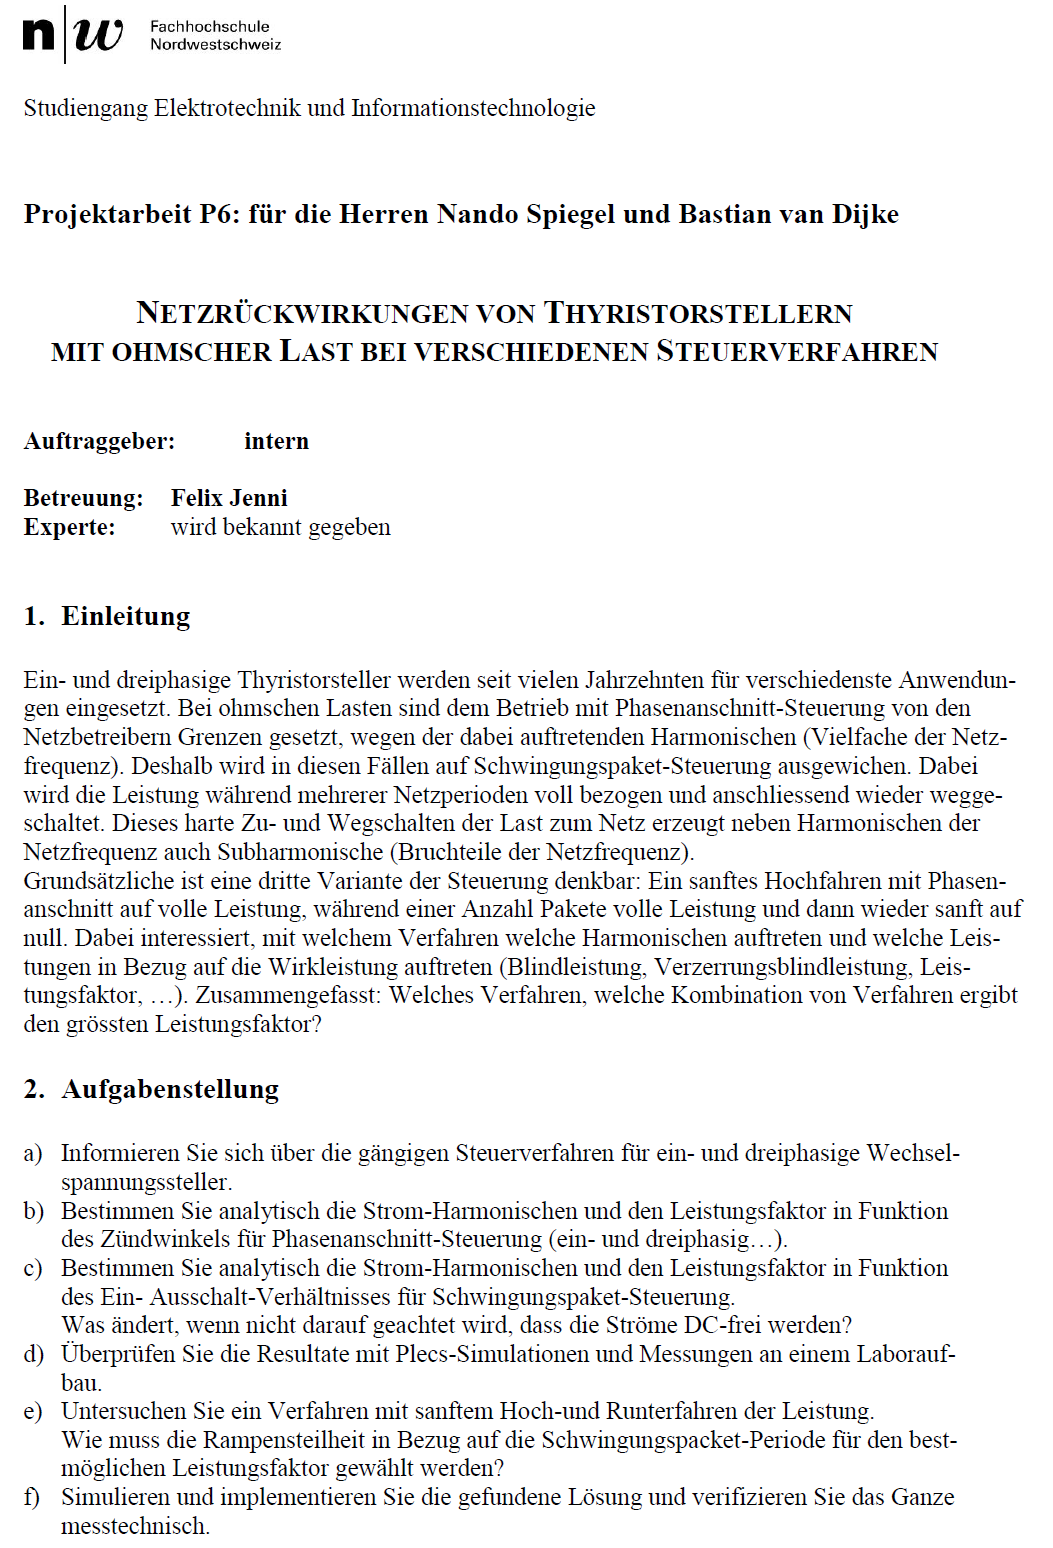
\includegraphics[width=0.95\textwidth]{Projekt_1.png}	
\end{figure}
\newpage
\begin{figure}[ht!]
	\centering
	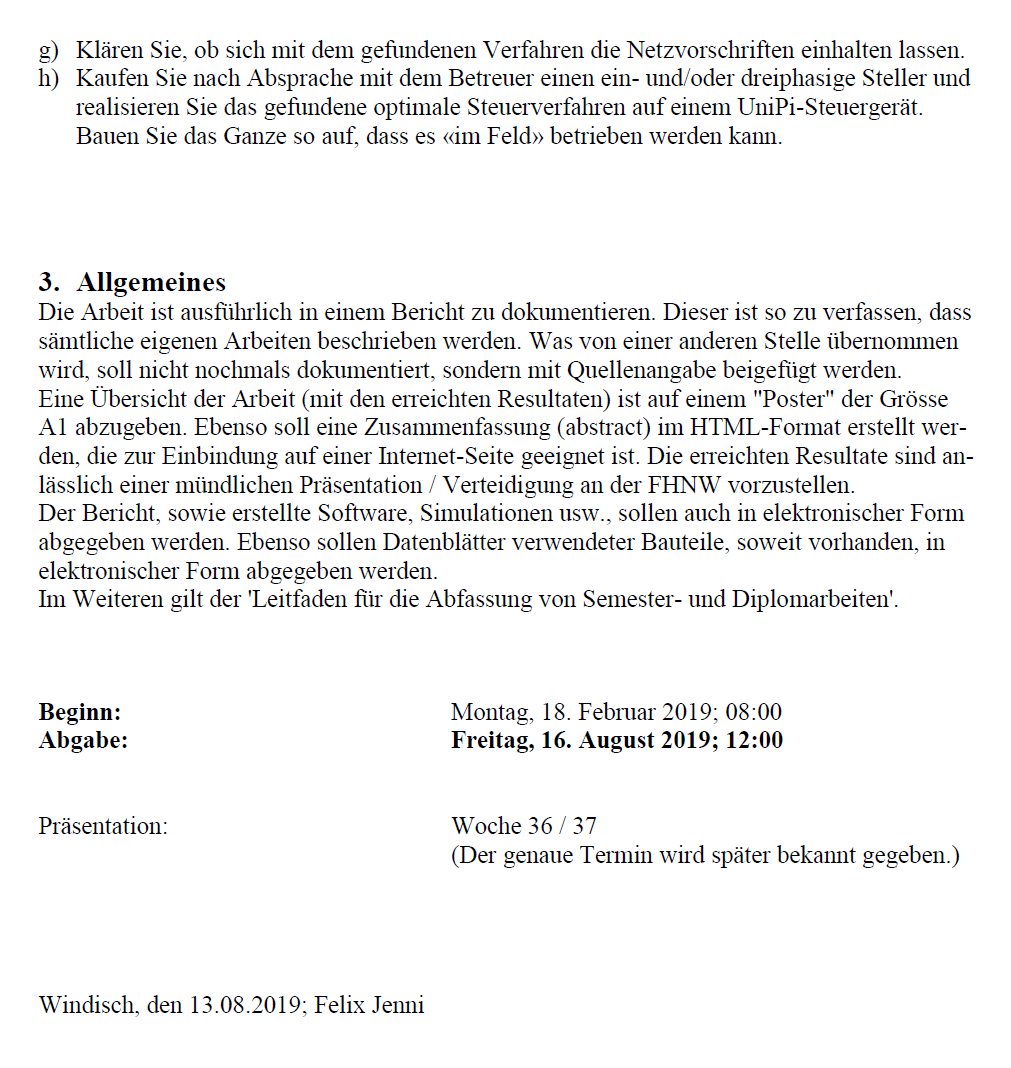
\includegraphics[width=0.95\textwidth]{Projekt_2.png}	
\end{figure}
\newpage
\section{Code}
\subsection{Matlab Berechnungen}
\subsection*{Leistungsfaktor}\label{sec:Leistungsfaktor_Berechnung}
\lstinputlisting{appendix/code/Leistungsfaktor.m}

\subsection*{Phasenanschnitt}\label{sec:Phasenanschnitt_Berechnung}
\lstinputlisting{appendix/code/FTT_Phasenanschnitt_final.m}

\subsection*{Schwingungspaket}\label{sec:Schwingungspaket_Berechnung}
\lstinputlisting{appendix/code/Schwingungspaketsteuerung_final.m}

\subsection*{Fourieranalyse von Hand}\label{sec:Fourieranalyse_Berechnung}
\lstinputlisting{appendix/code/Fourieranalyse_phasenanschnitt_final.m}

\subsection*{Trapez Funktion}\label{sec:Trapez_Berechnung}
\lstinputlisting{appendix/code/Trapez_funktion_final.m}

\subsection*{Leistungsfaktor der Messungen}\label{sec:Leistungsfaktor_Messungen}
\lstinputlisting{appendix/code/Leistungsfaktor_Messungen.m}

\subsection*{Spannungssignale mit FFT}\label{sec:Spannungen_Messungen}
\lstinputlisting{appendix/code/Berechnung_FFT_Widerstand.m}

\subsection*{Stromsignale mit FFT}\label{sec:Stroeme_Messungen}
\lstinputlisting{appendix/code/Berechnung_FFT_Stroeme_Widerstand.m}


\newpage
\subsection{Arduino-Programm}

\subsection*{Phasenanschnittsteuerung}
\begin{lstlisting}[basicstyle=\tiny,style=myArduino]
const int Switch_PO = 3;	// Output fuer den EIN- & AUSSCHALTER
const int Controll_P = 2;	// Output fuer Steuersignal
const int Switch_PI = 5;	// Input fuer den EIN- & AUSSCHALTER
int buttonState = 0;	// Zustand Schalter auf 0


void setup() {
pinMode (Switch_PO, OUTPUT);	// Schalter auf Output
pinMode (Controll_P, OUTPUT);	// PWM auf Output
pinMode (Switch_PI, INPUT_PULLUP);	// Schalter Eingang
}

void loop() {
analogWrite(Controll_P, 127); //Zuendwinkel ausgeben
}
\end{lstlisting}


\subsection*{Schwingungspaketsteuerung}
\begin{lstlisting}[basicstyle=\tiny,style=myArduino]
const int Switch_PO = 3;	// Output fuer den EIN- & AUSSCHALTER
const int Controll_P = 2;	// Output fuer Steuersignal
const int Switch_PI = 5;	// Input fuer den EIN- & AUSSCHALTER
int buttonState = 0;	// Zustand Schalter auf 0
int anzahl_Schwinwungspakete = 5;	// Anzahl Schwingungspakete

void setup() {
pinMode (Switch_PO, OUTPUT);	// Schalter auf Output
pinMode (Controll_P, OUTPUT);	// PWM auf Output
pinMode (Switch_PI, INPUT_PULLUP);	// Schalter Eingang
}

void loop() {
	buttonState =! digitalRead(Switch_PI);	// Da Pullup wird das Signal negiert
	if(buttonState == HIGH){	// if-Schleife falls Zustand Schalter auf EIN
		digitalWrite(Controll_P, HIGH);	// Auf High schalten um Zuendwinkel von 0 Grad zu erreichen (Volle Leistung)
		delay(800);	// Warten waehrend volle Leistung
		digitalWrite(Controll_P, LOW);	// Auf Low schalten um Zuendwinkel von 180 Grad zu erreichen (Keine Leistung)
		delay(200);// Genug Zeit zwischen den Paketen weil sonst wird eine Spannung von 0V nicht erreicht     
	}
}
\end{lstlisting}

\subsection*{Hartes Auf- und Absteuern}
\begin{lstlisting}[basicstyle=\tiny,style=myArduino]
const int Switch_PO = 3;	// Output fuer den EIN- & AUSSCHALTER
const int Controll_P = 2;	// Output fuer Steuersignal
const int Switch_PI = 5;	// Input fuer den EIN- & AUSSCHALTER

int buttonState = 0;	// Zustand Schalter auf 0
int anzahl_Schwingwungspakete = 5;	// Anzahl Schwingungspakete
int Geschwindigkeit = 5; //Steilheit des Hoch- und Runterfahrens

void setup() {
pinMode (Switch_PO, OUTPUT);	// Schalter auf Output
pinMode (Controll_P, OUTPUT);	// PWM auf Output
pinMode (Switch_PI, INPUT_PULLUP);	// Schalter Eingang
}

void loop() {
for (int z = 0; z < 10; z++) {	// for-Schleife fuer Schwingungspaketsteuerung
	if (z < anzahl_Schwingwungspakete) {	// Anzahl Schwingungen EIN
		for (int i = 0; i < 255; i++) {	// Hochfahren mit PWM
			analogWrite(Controll_P, i);	// Die Variable wird auf den Steuersignalausgang geschrieben
			delay(Geschwindigkeit);	// Geschwindigkeit des Hochfahrens
		}
		delay(200);	// Warten waehrend volle Leistung
		for (int i = 255; i > 0; i--) {	// Runterfahren mit PWM
			analogWrite(Controll_P, i);	// Die Variable wird auf den Steuersignalausgang geschrieben
			delay(Geschwindigkeit);	// Geschwindigkeit des Runterfahrens
		}
		delay(100);	// Warten waehrend keiner Leistung
		} else {
			digitalWrite(Controll_P, LOW);	// Ausschalten fuer Schwingungspakete keine Leistung
			delay((10 - anzahl_Schwingwungspakete) * 480);	// Verzoegerung bis wieder eingeschaltet werden soll
		}
	}
}
\end{lstlisting}

\newpage
\subsection*{Sanftes Auf- und Absteuern}
\begin{lstlisting}[basicstyle=\tiny,style=myArduino]
const int Switch_PO = 3;	// Output fuer den EIN- & AUSSCHALTER
const int Controll_P = 2;	// Output fuer Steuersignal
const int Switch_PI = 5;	// Input fuer den EIN- & AUSSCHALTER
int buttonState = 0;	// Zustand Schalter auf 0
int Geschwindigkeit = 75;	//Steilheit des Hoch- und Runterfahrens

void setup() {
	pinMode (Switch_PO, OUTPUT);  // Schalter auf Output
	pinMode (Controll_P, OUTPUT); // PWM auf Output
	pinMode (Switch_PI, INPUT_PULLUP);  // Schalter Eingang
}

void loop() {
	buttonState = ! digitalRead(Switch_PI);
	for (int i = 0; i < 255; i++) {	// Hochfahren mit PWM
		analogWrite(Controll_P, i);	// Die Variable wird auf den Steuersignalausgang geschrieben
		delay(Geschwindigkeit);	// Geschwindigkeit des Hochfahrens
	}
	delay(500);	// Warten waehrend volle Leistung
	for (int i = 255; i > 0; i--) {	// Runterfahren mit PWM
		analogWrite(Controll_P, i);	// Die Variable wird auf den Steuersignalausgang geschrieben
		delay(Geschwindigkeit);	// Geschwindigkeit des Runterfahrens
	}
	delay(2000);	// Warten waehrend keiner Leistung
}
\end{lstlisting}

\subsection*{Drehzahlregelung}\label{sec:Drehzahlregelung}
\begin{lstlisting}[basicstyle=\tiny,style=myArduino]
#define PIN_MESS A6 // Setzen Messpin
#define REF_VOLTAGE 5.0 // Setzen Referenzspannung
#define PIN_STEPS 1024.0  // Setzen ADC
const int Switch_PO = 3;  // Output fuer den EIN- & AUSSCHALTER
const int Controll_P = 2; // Output fuer Steuersignal
const int Switch_PI = 5;  // Input fuer den EIN- & AUSSCHALTER
int buttonState = 0;  // Zustand Schalter auf 0
float vout = 0.0, vin = 0.0;  // Definieren Ein- und Ausgangsspannung
float R1 = 611000.0; // resistance R1 (= 611 KOhm)
float R2 =  56000.0; // resistance R2 (= 56 KOhm)
float rawValue = 0; // Definieren ADC Wert
float Vsoll = 40; //Sollspannung vorgeben
float Vaus = Vsoll / 60 * 255; // Sollspannung umrechnen
float Vdiff = 0.0;  // Definieren Differenzspannung
float Vdiff_255 = Vdiff / 60 * 255; // Differenzspannung umrechnen
float Vdiff_1 = 0.0;  // Definieren Differenzspannung von letztem Durchgang
float Vaus_1 = 0.0; // Definieren Ausgangsspannung von letztem Durchgang
float Ti = 0.0003453873519; // Zeit PI-Regler
float  Kp = 0.1;  // Proportinal Faktor PI-Regler
float  Ki = 0.01; // Integral Faktor PI-Rgler
float  B_0 = Kp + Ki * Ti / 2; // Definieren B0
float  B_1 =  -Kp + Ki * Ti / 2;  // Definieren B1
float Vausgabe = Vausdifferenz / 60 * 255; // Definieren endgueltige Ausgangsspannung
float Vausdifferenz = 0; //  Definieren endgueltige Differenzspannung
float Vauslog = Vaus / 255 * 60; // Umrechnen Ausgangsspannung

void setup() {
	pinMode (Switch_PO, OUTPUT);  // Schalter auf Output
	pinMode (Controll_P, OUTPUT); // PWM auf Output
	pinMode (Switch_PI, INPUT_PULLUP);  // Schalter Eingang
	Serial.begin(9600); // Schreibrate
	pinMode(PIN_MESS, INPUT); // Messung auf Input
}

void loop() {
	buttonState =! digitalRead(Switch_PI);  // Da Pullup wird das Signal negiert
	if(buttonState == HIGH){  // if-Schleife falls Zustand Schalter auf EIN
		rawValue = analogRead(PIN_MESS); // Auslesen ADC
		vout = (rawValue * REF_VOLTAGE) / PIN_STEPS;  // Umrechnen auf 5V
		vin = vout / (R2 / (R1 + R2));  // Umrechnen auf 60V
		
		Vdiff = Vsoll - vin;  // Berechnen Differenzspannung
		Vaus = Vaus_1 + B_0 * Vdiff + B_1 * Vdiff_1;  // Berechnen Ausgangsspannung mit Filter
		Vausdifferenz = Vauslog + Vdiff_255;  // Berechnen Differenzspannung und Ausgangsspannung
		
		if (Vausgabe > 255) { // Begrenzung auf 255 Werte
			Vausgabe = 255;
		}
		if (Vausgabe < 0) { // Begrenzung negativer Bereich
			Vausgabe = 0;
		}	
		analogWrite(Controll_P, Vausgabe);  // Ausgeben von Ausgangsspannung
		Vdiff_1 = Vdiff;  // Differenzspannung in Differenzspannung von letztem Durchgang laden
		Vaus_1 = Vausgabe;  // Ausgangsspannung in Ausgangsspannung von letztem Durchgang laden
	}
	delay(10);  // Abtastrate definieren
}
\end{lstlisting}

\newpage
\section{Zusammenfassung der Normen}\label{sec:Zusammenfassung_Normen}

\subsubsection{EN 61000-3-2 Grenzwerte für Oberschwingungsströme}\label{sec:Stromnormen_ZF}
Diese Norm gilt für elektrische und elektronische Geräte (Betriebsmittel und Einrichtungen) bis zu einem Eingangsstrom von \SI{16}{A} je Leiter. Ausserdem ist der Anschluss des Gerätes an das öffentliche Niederspannungsverteilnetz vorgesehen. Unter dem Begriff \grqq Elektrische Einrichtung\grqq versteht man eine Anlage, welches aus einem oder mehreren voneinander unabhängigen Geräten besteht. Sie bilden eine elektrische Einrichtung, wenn nur durch deren Zusammenwirken der bestimmungsgemässe Zweck der Einrichtung erzielt werden kann. Ein Beispiel für eine elektrische Einrichtung ist, der Treppenlichtautomat zusammen mit den dazugehörigen Leuchten. Nur der Automat ohne Beleuchtung erfüllt den technischen Zweck der Bezeichnung nicht. Ein weiteres Beispiel für eine \grqq Elektrische Einrichtung \grqq wäre der motorische Antrieb. Aber auch hier gilt, dass der Motor ohne mechanische Last den technischen Nutzen nicht erfüllen würde.\\
Die Norm definiert die Grenzwerte der Oberschwingungsanteile des Eingangsstromes bis zur 40. Harmonischen, die durch ein Gerät hervorgerufen werden können, dass unter festgelegten Bedingungen geprüft wird. Da heutzutage die Zahl der nicht linearen Verbraucher am öffentlichen Versorgungsnetz zunehmend steigen, steigt auch der Anteil des Oberschwingungsgehalts der Versorgungsspannung. Die nicht-sinusförmige und somit oberschwingungsbehaftete Stromentnahme verursacht an der Netzimpedanz Spannungsabfälle. Das Resultat ist eine Abweichung des Spannungsverlaufs von dem idealen harmonischen Verlauf des Netzes. Um normgerechte und reproduzierbare Messungen der Stromoberschwingungen durchführen zu können, muss ein ideales oberschwingungsfreies Netz zur Verfügung stehen. Laut der Norm EN 61000-3-2 darf die Prüfquelle eine bestimmten Oberwellengehalt nicht überschreiten. Es muss sichergestellt werden, dass ausschliesslich die vom Verbraucher erzeugte Stromoberschwingung gemessen werden. Beginnt man mit der Prüfung, muss der Prüfling so eingestellt werden, dass der höchste Gesamt-Oberschwingungsstrom (maximal total harmonic current) unter üblichen Betriebsbedingungen erreicht wird. Für die Quellenanforderung gelten folgende Spezifikationen, die zwingend während des zu prüfenden Geräts eingehalten werden müssen:

\begin{itemize}
	\item Spannungsgenauigkeit $\pm$ 2 \%
	\item Frequenzgenauigkeit $\pm$ 0.5 \%
	\item Phasenwinkelstabilität $\pm$ $1.5^\circ$
	\item 	U$_{peak}$ = \SI{1.4}{V} - \SI{1.42}{V} U$_{eff}$ und zwischen 87\textdegree \hspace{0.02cm} und 93\textdegree \hspace{0.02cm} muss nach dem Nulldurchgang erreicht werden. dies muss jedoch nicht eingehalten werden, sofern Klasse A oder B geprüft wird.
	\item Die relativen Oberschwingungsanteile der Prüfspannung dürfen folgende Werte nicht überschreiten:\\
	0.9 \% für die 3. Harmonische Oberschwingung\\
	0.4 \% für die 5. Harmonische Oberschwingung\\
	0.3 \% für die 7. Harmonische Oberschwingung\\
	0.2 \% für die 9. Harmonische Oberschwingung\\
	0.2 \% für die geradzahlige Oberschwingung 2 bis 10 Ordnung\\
	0.1 \% für die Oberschwingung 11 bis 40 Ordnung\\
\end{itemize} 

In der Norm 61000-3-2 sind 4 Geräteklassen definiert, bei denen die Oberschwingungen des Eingangsstromes die Werte nicht überschreiten dürfen. Da es sich beim vorliegenden Projekt um symmetrische, dreiphasige ohmsche Lasten handelt, fällt dies unter die Klasse A. Ausserdem beinhalten die folgenden Einrichtungen auch die Klasse A. 
\begin{itemize}
	\item Symmetrische dreiphasige Geräte	
	\item Haushaltsgeräte (ausser die, die in Klasse D fallen)
	\item Elektrowerkzeuge (ausser tragbare Elektrowerkzeuge)
	\item Beleuchtungsregler (Dimmer) für Glühlampen
	\item Audio-Einrichtungen
\end{itemize} 

Um zu verdeutlichen, welche Geräte die anderen Klasse erhalten, sind sie der Vollständigkeit halber aufgelistet.\\
Klasse B:
\begin{itemize}
	\item tragbare Elektrowerkzeuge 	
	\item Lichtbogenschweisseinrichtungen, die nicht zum professionellen Gebrauch vorgesehen sind.
\end{itemize} 
Klasse C:
\begin{itemize}
	\item Beleuchtungseinrichtungen	
\end{itemize} 
Klasse D:
\begin{itemize}
	\item Personalcomputer und Bildschirme (Monitore) für Personalcomputer	
	\item Fernseh-Rundfunkempfänger
\end{itemize}

Falls es Geräte gibt, die nicht in die Klassen B bis D fallen, müssen sie automatisch als Geräte der Klasse A definiert werden.\\
Die Grenzwerte für den Höchstwert des Oberschwingungsstromes für Klasse A Geräte sind wie folgt definiert:

\begin{table}[ht!]
	\centering
	\begin{tabular}{|l|l|}
		\hline
		\multicolumn{1}{|c|}{Oberschwingungsordnung} & \multicolumn{1}{c|}{\begin{tabular}[c]{@{}c@{}}Zuverlässiger Höchstwert des \\ Oberschwingungsstromes\end{tabular}} \\
		\multicolumn{1}{|c|}{\textit{n}}                      & \multicolumn{1}{c|}{A}                                                                                              \\ \hline
		\multicolumn{2}{|c|}{Ungeradzahlige Oberschwingungen}                                                                                                              \\ \hline
		3                                            & 2.30                                                                                                                \\
		5                                            & 1.14                                                                                                                \\
		7                                            & 0.77                                                                                                                \\
		9                                            & 0.40                                                                                                                \\
		11                                           & 0.33                                                                                                                \\
		13                                           & 0.21                                                                                                                \\
		15 $\leq$ \textit{n} $\leq$ 39               & 0.15 x 15/\textit{n}                                                                                                \\ \hline
		\multicolumn{2}{|c|}{Geradzahlige Oberschwingungen}                                                                                                                \\ \hline
		2                                            & 1.08                                                                                                                \\
		4                                            & 0.43                                                                                                                \\
		6                                            & 0.30                                                                                                                \\
		8 $\leq$ \textit{n} $\leq$ 40                & 0.23 x 8/\textit{n}                                                                                                 \\ \hline
	\end{tabular}
	\caption{Grenzwerte für Geräte der Klasse A}\label{tab:Grenzwerte_Normen_ZF}
\end{table}


Ein weiterer wichtiger Wert ist die jeweilige Beobachtungsdauer der Endgeräte. Es sind hier verschiedene Arten von Geräteverhalten definiert und dabei die Beobachtungsdauer bestimmt. Dies sieht man in der folgenden Tabelle \ref{tab:Beobachtungsdauer_für_die_Prüfung} \cite{EMVNorm}.

\begin{table}[ht!]
	\centering
	\begin{tabular}{|l|l|}
		\hline
		\multicolumn{1}{|c|}{Art des Geräteveraltens}                      & \multicolumn{1}{c|}{Beobachtungsdauer}                                                                                                                                                                                   \\ \hline
		quasi-stationär                                                    & \begin{tabular}[c]{@{}l@{}}T$_{obs}$ von ausreichender Dauer, um die Anforderungen\\ zur Wiederholpräzision einzuhalten\end{tabular}                                                                                          \\ \hline
		kurzer Zyklus (T$_{cycle}$ $\leq$ 2.5min)                                    & \begin{tabular}[c]{@{}l@{}}T$_{obs}$ $\geq$ 10 Zyklen (Bezugsverfahren) oder T$_{obs}$ von \\ ausreichender Dauer oder Synochronisation, um \\ die Anforderungen zur Wiederholpräzision\\ einzuhalten \hspace{0.1cm}$^a$\end{tabular}                      \\ \hline
		zufällig                                                           & \begin{tabular}[c]{@{}l@{}}T$_{obs}$ von ausreichender Dauer, um die Anforderungen\\ zur Wiederholpräzision einzuhalten\end{tabular}                                                                                          \\ \hline
		langer Zyklus (T$_{cycle}$ \textgreater 2.5 min)                        & \begin{tabular}[c]{@{}l@{}}voller Programmzyklus des Gerätes (Bezugsverfahren)\\ oder ein repräsentives 2.5 min -Intervall mit dem \\ höchsten THC angesehen wird\end{tabular}                                           \\ \hline
		\multicolumn{2}{|l|}{\begin{tabular}[c]{@{}l@{}} $^a$ \grqq Synchronisation\grqq \hspace{0.08cm} bedeutet, dass die gesamte Beobachtungsdauer hinreichend gut eine\\ exakte ganzzahlige Anzahl von Betriebszyklen des Gerätes umfasst, so dass die\\Anforderungen zur Wiederholpräzision eingehalten wird.\end{tabular}} \\ \hline
	\end{tabular}
	\caption{Beobachtungsdauer für die Prüfung}\label{tab:Beobachtungsdauer_für_die_Prüfung}
\end{table}


\subsubsection{EN 61000-3-3 Begrenzung von Spannungsänderungen, Spannungsschwankungen} \label{sec:flickernorm}
Auch diese Norm gilt für Geräte und Einrichtungen mit einem Nenn-Eingansstrom von bis zu \SI{16}{A} je Aussenleiter, die zum Anschluss an das öffentliche Niederspannungsnetz vorgesehen sind und keiner Sonderanschlussbedingung unterlegen. Die Flicker, die auch als repetitive Spannungsänderungen bekannt sind, können so begrenzt werden. Falls Geräte und Einrichtungen diese Norm erfüllen, dürfen sie ohne weitere Prüfung an jeden Anschlusspunkt des öffentlichen Netzes angeschlossen werden. Die Nennleistung, welche die Geräte und Einrichtungen aufweisen sollten, sind ohne Einschränkungen kleiner als \SI{11}{kW} bei Drehstromgeräten, \SI{3.7}{kW} bei Einphasengeräten und \SI{6.47}{kW} bei Zweiphasengeräten. Diese Norm trifft man unter anderem beifolgenden Geräten an:
\begin{itemize}
	\item Haushaltsgeräte und tragbare Elektrowerkzeuge 
	\item Motorbetriebene Geräte (Waschmaschine, Staubsauger, Elektrowärmegerät und Kocheinrichtungen)
	\item Beleuchtungseinrichtungen
	\item Automatische elektrische Steuerungen für Hausgebrauch und ähnliche Anwendungen
	\item Drehzahlgeregelte Antriebe
	\item Funk-Einrichtungen
	\item Lichtbogenschweisseinrichtungen
	\item Medizinische Geräte und Einrichtungen
	\item Mikrowellengeräte	
\end{itemize}

Die Norm schreibt eine Prüfung der zu beurteilenden Geräten, an einer Prüfungsimpedanz vor. Die Impedanz $Z$ ist in Abbildung \ref{fig:Bezugsimpedanz} als Widerstand R$_A$ in Serie mit einer Spule jX$_A$ dargestellt und entspricht den folgenden Werten:


\begin{figure}[ht!]
	\centering
	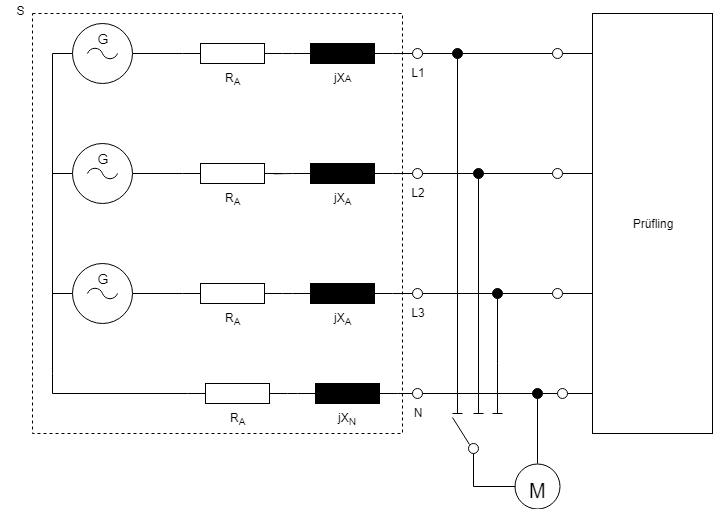
\includegraphics[scale=0.4]{Bezugsimpedanz.png}	
	\caption{Prüfspannungsquelle mit der Bezugsimpedanz}
	\label{fig:Bezugsimpedanz}
\end{figure}

\begin{table}[ht!]
	\begin{tabular}{ll}
		G  & Spannungsquelle                                                                                                                                                                                                                                               \\
		M  & Messeinrichtung                                                                                                                                                                                                                                               \\
		S  & \begin{tabular}[c]{@{}l@{}}Prüfungspannungsquelle, bestehend aus dem Spannungsgenerator  G und der\\ Bezugsimpedanz Z mit den Elemente\end{tabular}                                                                                                           \\
		& \begin{tabular}[c]{@{}l@{}}R$_A$ = $\SI{0.24}{\Omega}$  jX$_A$ = $\SI{0.15}{\Omega}$ bei $\SI{50}{Hz}$\\ R$_N$ = $\SI{0.16}{\Omega}$ jX$_A$ = $\SI{0.10}{\Omega}$ bei $\SI{50}{Hz}$\end{tabular}
	\end{tabular}
\end{table}

Die drei Quellenspannungen $G$ entsprechen der Nennspannung. Alle Spannungen werden auf die Nennspannung $Un$ normiert: Der Prüfkreis besteht aus der Prüfspannungsquelle, dem zu prüfenden Gerät (Prüfling) und einer Messeinrichtung, zum Beispiel Strommesser, Spannungszange oder einem Flickermeter (M).\\
Es gibt bei der Bezugsimpedanz keine Unterscheidung im Anwendungsbereich zwischen Haushaltsgeräten und gewerblich genutzten Geräten. Stattdessen wird die Langzeit-Flickerstärke eingeführt und auf 65 \% der Kurzzeit-Flickerstärke begrenzt \cite{FlickerNorm}.\\
Damit man versteht, welche Bedeutung der Flickerwert hat und wie er zustande gekommen ist, gibt es hier eine Kurze Erklärung des Begriffes:\\
Mithilfe des Flickerwertes kann man die Störempfindlichkeit des menschlichen Auges, auf Helligkeitsschwankungen bei der Beleuchtung, durch einen messbaren Wert ermitteln. Dieser Wert ist eine dimensionslose Zahl, welche das Störempfinden des Menschen ausdrückt, wenn er sich mit einer \SI{60}{W}-Glühbirne beleuchtet. Die Helligkeit variiert dabei auf Grund von Spannungsschwankungen. Erhält man den Wert 0, so bedeutet dies, dass praktisch keine Schwankungen der Spannungshöhe vorhanden und somit auch kein Flackern der Lampe ersichtlich ist.\\
Bei dem Wert 1 gibt es eine gewisse Helligkeitsschwankung, die als störend wahrgenommen wird. Jedoch sind die Resultate nicht aussagekräftig, da sie Orts-, Zeit- und Personen abhängig sind. Deshalb entwickelte man einen Algorithmus und ein entsprechendes Formelwerk für das Durchschnittsempfinden der Erkenntnisse. Mit Hilfe eines Flicker-Meters konnte ein geeignetes Messgerät entwickelt werden, welches mit einem Flickermessverfahren den Flickerwert berechnen konnte. Das Flicker-Meter liefert alle 10 Minuten einen Wert, der mit $Pst$ bezeichnet wird. Das $P$ steht dabei für $perceptibility units$ (Wahrnehmungseinheiten) und $st$ steht für $short time$. Der Wert, welcher man behandelt ist also der Kurzzeit-Flickerwert.\\
Die EN 50160-Norm sagt aus, dass man 12 aufeinander folgende $Pst$-Werte zusammenfassend zu einem $Plt$-Wert (long time-Flicker = Langzeit-Flicker) verrechnen kann. Genauer bedeutet dies, dass man die 12 $Pst$-Werte, die über 2 Stunden gemessen wurden, zusammenrechnet und daraus den Durchschnitt nimmt. Jeder einzelne $Pst$-Wert geht mit einer 3. Potenz in die Bewertung ein. Der $Plt$-Wert ist der kubische Mittelwert der 12 $Pst-Werte$ und ist in der unterstehenden Formel dargestellt \cite{Spannungsqualitaet}.

\begin{equation}\label{eq:Plt}
P_{lt} = {\sqrt[3]{\frac{\sum_{i=1}^{N} {P_{st,i}}^3}{N}}}
\end{equation}

Mithilfe dieser Norm können Typenprüfung für bestimmte Geräte vorgenommen werden. Das Ziel dieser Typenprüfung ist es, die Übereinstimmung mit den Grenzwerten festzustellen. Diese werden unter Laborbedingungen an einem Bezugsnetz betrieben. Bei den festgelegten Betriebsbedingungen werden die erzeugten Spannungsschwankungen in Bezug zu den Bezugsimpedanzen gemessen und beurteilt. Falls Geräte die Grenzwerte dieser Norm einhalten, kann davon ausgegangen werden, dass sie zu keinerlei Beschwerden im Netz Anlass geben. Die elektromagnetische Verträglichkeit ist daher gewährleistet \cite{FlickerNorm}. 


\subsubsection{EN 61000-2-2 Grenzwerte für Oberschwingungsspannungen}

Die folgende Norm beinhaltet die Festlegung für Verträglichkeitspegel von niederfrequenten, leitungsgeführten Störgrössen und für Signale von Netz-Kommunikationssystemen in öffentlichen Niederspannungs- und Stromversorgungsnetzen. Die Werte des Verträglichkeitspegels mit ihrer Eigenschaft können für die EMV-Koordinierung von Störaussendungs- und Störfestigkeitsanforderungen für Geräte und als Planungspegel für Stromversorgungsnetze verwendet werden. In der Norm werden folgende Phänomene betrachtet:

\begin{itemize}
	\item Spannungsschwankungen und Flicker 
	\item Oberschwingungen bis zur 50. Oberschwingungsordnung
	\item Zwischenharmonische
	\item Spannungsverzerrungen bei Frequenzen oberhalb der 50. Oberschwingungsordnung
	\item Spannungseinbrüche
	\item Kurzzeitunterbrechungen der Versorgungsspannung
	\item Spannungsunsymmetrien
	\item Kurzzeitunterbrechungen der Versorgungsspannung
	\item Transiente Überspannung
	\item Zweiteilige Schwankung der Netzfrequenz
\end{itemize}
Wobei man sagen kann, dass einige Punkt, wie zum Beispiel das Bestimmen des Flickerwertes oder die Langzeit- und die Kurzzeit Flickerstärke schon in der vorherigen Norm definiert sind.\\
Die Tabelle \ref{tab:kompatibilitätsstufen_ZF} zeigt die verschiedenen Kompatibilitätsstufen für einzelne Oberschwingungsspannungen im Niederspannungsnetz. Sie ist nur in Bezug auf Langzeiteffekte für einzelne harmonische Spannung definiert. Der Wert der gesamten harmonische Verzerrung darf hierbei höchstens einen Wert von $THD$ = 8\% betragen im stationären Betrieb.
\begin{table}[ht!]
	\centering
	\resizebox{\textwidth}{!}{%
		\begin{tabular}{|l|l|l|l|l|l|}
			\hline
			\multicolumn{2}{|c|}{\begin{tabular}[c]{@{}c@{}}Ungeradzahlige \\ Harmonische \\ nicht-vielfache von 3\end{tabular}}                                                            & \multicolumn{2}{c|}{\begin{tabular}[c]{@{}c@{}}Ungeradzahlige \\ Harmonische \\ Vielfache von 3\end{tabular}}                                                                     & \multicolumn{2}{c|}{\begin{tabular}[c]{@{}c@{}}Geradzahlige \\ Harmonische\end{tabular}}                                                                                          \\ \hline
			\multicolumn{1}{|c|}{\begin{tabular}[c]{@{}c@{}}Oberschwingungs\\ -ordnung\end{tabular}} & \multicolumn{1}{c|}{\begin{tabular}[c]{@{}c@{}}Harmonische \\ Spannung\end{tabular}} & \multicolumn{1}{c|}{\begin{tabular}[c]{@{}c@{}}Oberschwingungs\\ -ordnung\end{tabular}} & \multicolumn{1}{c|}{\begin{tabular}[c]{@{}c@{}}Harmonische \\ Spannung\end{tabular}} & \multicolumn{1}{c|}{\begin{tabular}[c]{@{}c@{}}Oberschwingungs\\ -ordnung\end{tabular}} & \multicolumn{1}{c|}{\begin{tabular}[c]{@{}c@{}}Harmonische \\ Spannung\end{tabular}} \\
			\multicolumn{1}{|c|}{\textit{h}}                                                                  & \multicolumn{1}{c|}{\%}                                                              & \multicolumn{1}{c|}{\textit{h}}                                                                     & \multicolumn{1}{c|}{\%}                                                              & \multicolumn{1}{c|}{\textit{h}}                                                                     & \multicolumn{1}{c|}{\%}                                                              \\ \hline
			
			5                                                         & 6                                                     & 3                                                       & 5                                                & 2                                           & 2                                         \\
			7                                                         & 5                                                     & 9                                                       & 1.5                                              & 4                                           & 1                                         \\
			11                                                        & 3.5                                                   & 15                                                      & 0.4                                              & 6                                           & 0.5                                       \\
			13                                                        & 3                                                     & 21                                                      & 0.3                                              & 8                                           & 0.5                                       \\
			17 $\leq$\textit{h}$\leq$ 49                                                   & 2.27x(17/\textit{h})-0.27                                   & 21<h$\leq$45                                                 & 0.2                                              & 10$\leq$\textit{h}$\leq$50                                     & 0.25x(10/\textit{h})+0.25                       \\ \hline
	\end{tabular}}
	\caption{Kompatibilitätsstufen für einzelne Oberschwingungsspannungen im Niederspannungsnetz}\label{tab:kompatibilitätsstufen_ZF}
\end{table}

Bei Kurzzeiteffekten wird ein Faktor k zu den harmonischen Ordnungen hinzu multipliziert. Dieser Faktor wird wie folgt berechnet: 
\begin{equation}\label{eq:factor_k_für_kurzzeiteffekte_ZF}
k = {1.3+\frac{0.7}{45}\cdot(h-5)}
\end{equation}
Der entsprechende Kompatibilitätsgrad für die gesamte harmonische Verzerrung liegt daher bei $THD$ = 11\%.



Die Tabelle \ref{tab:subharmonische_Spannung_ZF} zeigt die erforderlichen Werte in Prozent der subharmonischen Spannung im Niederspannungsnetz bei \SI{230}{V}, bei einer Frequenz von \SI{10}{Hz} bis \SI{90}{Hz}. Sie entsprechen dem Kompatibilitätsgrad bezüglich des Flimmerns.
\begin{table}[ht!]
	\centering
	\begin{tabular}{|l|l|l|}
		\hline
		\multicolumn{1}{|c|}{\multirow{3}{*}{\begin{tabular}[c]{@{}c@{}}Ordnung\\   {[}m{]}\end{tabular}}} & \multicolumn{2}{c|}{50 Hz System}                                                                                                                    \\ \cline{2-3} 
		\multicolumn{1}{|c|}{}                                                                             & \multicolumn{1}{c|}{\multirow{2}{*}{\begin{tabular}[c]{@{}c@{}}Subharmonische\\   Frequenzen fm {[}Hz{]}\end{tabular}}} & \multicolumn{1}{c|}{Um \%} \\ \cline{3-3} 
		\multicolumn{1}{|c|}{}                                                                             & \multicolumn{1}{c|}{}                                                                                                   & \multicolumn{1}{c|}{230V}  \\ \hline
		0.20 < m $\leq$ 0.60                                                                              & 10 < fm $\leq$ 30                                                                                                    & 0.51                        \\ \hline
		0.60 < m $\leq$ 0.64                                                                             & 30 < fm $\leq$ 32                                                                                                    & 0.43                        \\ \hline
		0.64 < m $\leq$ 0.68                                                                            & 32 < fm $\leq$ 34                                                                                                    & 0.35                        \\ \hline
		0.68 < m $\leq$ 0.72                                                                            & 34 < fm $\leq$ 36                                                                                                    & 0.28                        \\ \hline
		0.72 < m $\leq$ 0.76                                                                            & 36 < fm $\leq$ 38                                                                                                    & 0.23                        \\ \hline
		0.76 < m $\leq$ 0.84                                                                            & 38 < fm $\leq$ 42                                                                                                    & 0.18                        \\ \hline
		0.84 < m $\leq$ 0.88                                                                            & 42 < fm $\leq$ 44                                                                                                    & 0.18                        \\ \hline
		0.88 < m $\leq$ 0.92                                                                            & 44 < fm $\leq$ 46                                                                                                    & 0.24                        \\ \hline
		0.92 < m $\leq$ 0.96                                                                            & 46 < fm $\leq$ 48                                                                                                    & 0.36                        \\ \hline
		0.96 < m $\leq$ 1.04                                                                            & 48 < fm $\leq$ 52                                                                                                    & 0.64                        \\ \hline
		1.04 < m $\leq$ 1.08                                                                            & 52 < fm $\leq$ 54                                                                                                    & 0.36                        \\ \hline
		1.08 < m $\leq$ 1.12                                                                            & 54 < fm $\leq$ 56                                                                                                    & 0.24                        \\ \hline
		1.12 < m $\leq$ 1.16                                                                            & 56 < fm $\leq$ 58                                                                                                    & 0.18                        \\ \hline
		1.16 < m $\leq$ 1.24                                                                            & 58 < fm $\leq$ 62                                                                                                    & 0.18                        \\ \hline
		1.24 < m $\leq$ 1.28                                                                            & 62 < fm $\leq$ 64                                                                                                    & 0.23                        \\ \hline
		1.28 < m $\leq$ 1.32                                                                            & 64 < fm $\leq$ 66                                                                                                    & 0.28                        \\ \hline
		1.32 < m $\leq$ 1.36                                                                            & 66 < fm $\leq$ 68                                                                                                    & 0.35                        \\ \hline
		1.36 < m $\leq$ 1.40                                                                             & 68 < fm $\leq$ 70                                                                                                    & 0.43                        \\ \hline
		1.40 < m $\leq$ 1.80                                                                              & 70 < fm $\leq$ 90                                                                                                    & 0.51                        \\ \hline
	\end{tabular}
	\caption{Erforderlichen Werte der subharmonischen Spannungen}\label{tab:subharmonische_Spannung_ZF}
\end{table}

Einige Effekte, die wegen subharmonische Oberschwingung entstehen können sind:
\begin{itemize}
	\item Unerwünschter Strom, der in die Versorgungsnetze fliesst, welcher zusätzlicher Energieverlust verursacht.
	\item Subharmonische Spannungen stören den Betrieb von Leuchtstofflampen und anderen elektronischen Geräte, wie zum Beispiel Fernsehempfängern. Jede Verwendung von Strom und Spannungen, bei der die Höhe der Amplitude oder der Zeitpunkt des Nulldurchgangs wichtig ist, kann somit gestört werden, wenn die Kombination der vorhandenen unerwünschten Frequenz diese Eigenschaften der Versorgungsspannung ändern.
	\item Je grösser der Frequenzbereich ist und je grösser die Amplitude der Spannung bei diesen Frequenzen sind, desto grösser ist das Risiko unvorhersehbare Resonanzeffekte zu erhalten. Sie verstärkt die Spannungsverzerrung der Versorgungsspannung und führen zu einer Überlast oder anderen Störung bei den elektrischen Verbrauchern.
	\item Ein weiterer Effekt ist das Erzeugen von akustischen Geräuschen. Dies tritt jedoch vor allem bei einem Frequenzbereich von \SI{1}{kHz} bis \SI{9}{kHz} auf, bei der die Amplitude 0.5\% vom Frequenzwert abweicht und von der Art des beeinflussten Gerätes \cite{SpannungsNorm}.
\end{itemize}

\newpage
\section{Vergleich der Resultate von Plecs und Matlab}\label{sec:Vergleich_der_Resultate}

\begin{figure}[ht!]
	\centering
	\subfloat[][]{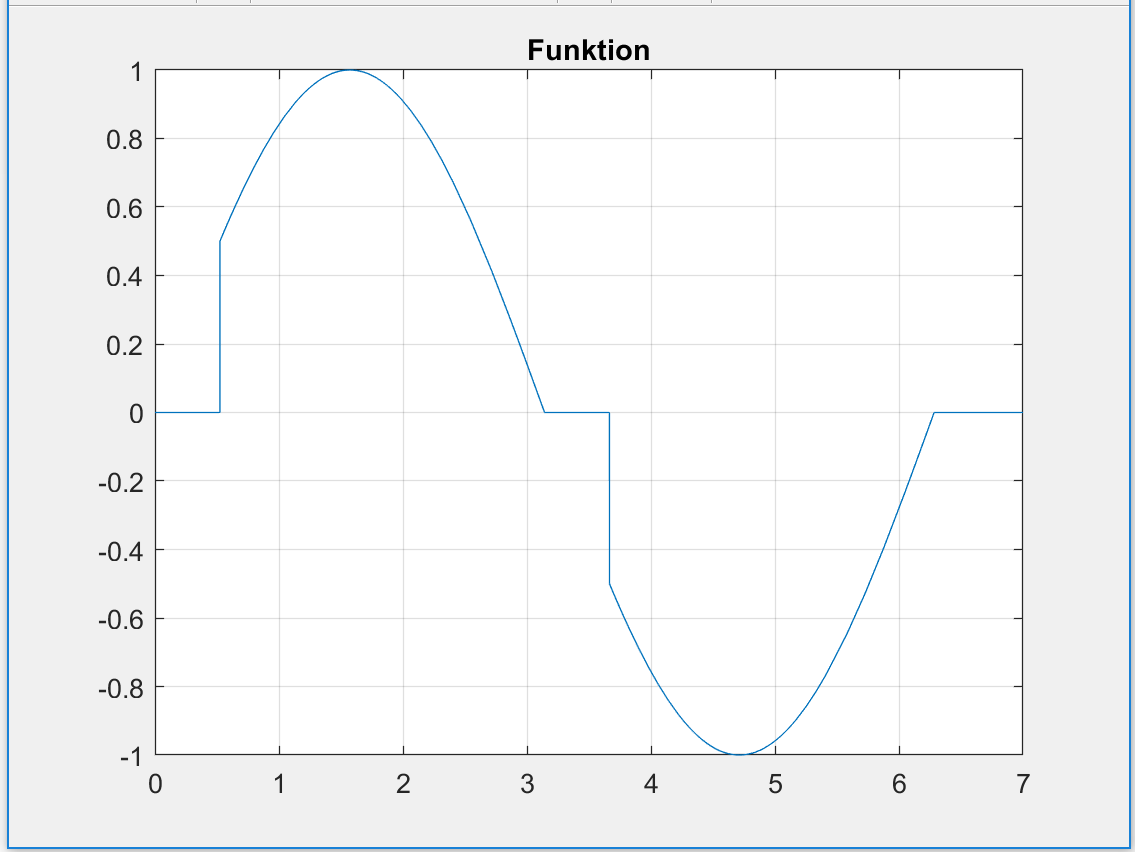
\includegraphics[width=0.4\linewidth]{eingangssignal_30.png}\label{fig:eingangssignal_30}}\qquad
	\subfloat[][]{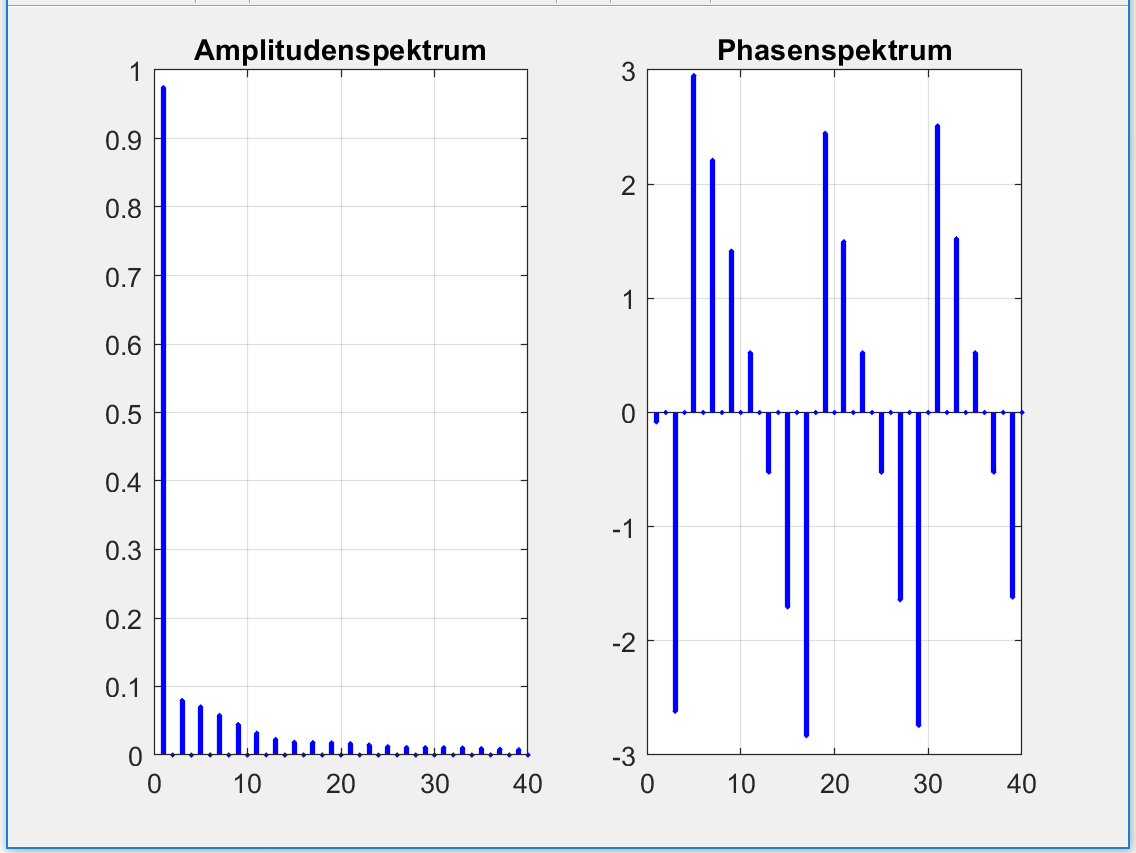
\includegraphics[width=0.4\linewidth]{A_PH_30.png}\label{fig:A_PH_30.}}
	\caption{Phasenanschnittsteuerung mit 30\textdegree (a) Eingangssignal (b) Amplituden- und Phasenspektrum}
	\label{fig:Phasenanschnittsteuerung_mit_30}
\end{figure}

\begin{figure}[ht!]
	\centering
	\subfloat[][]{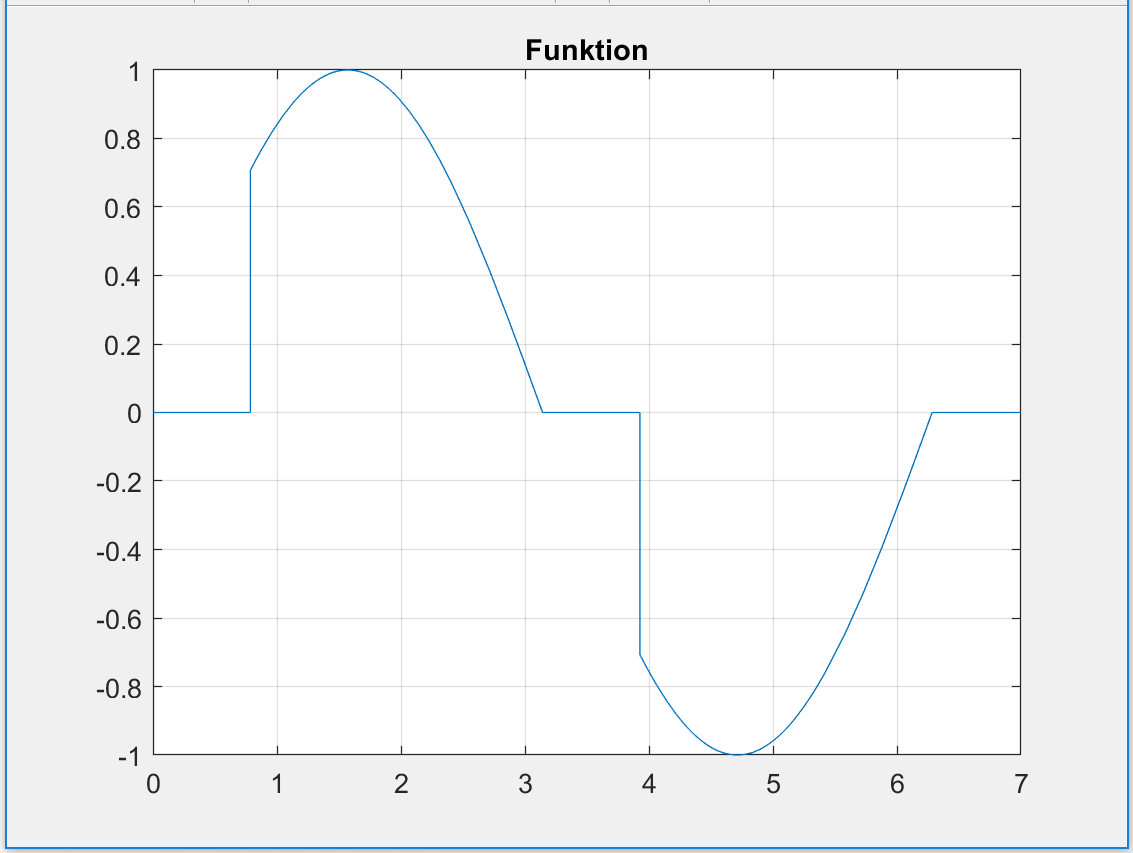
\includegraphics[width=0.4\linewidth]{eingangssignal_45.png}\label{fig:eingangssignal_45}}\qquad
	\subfloat[][]{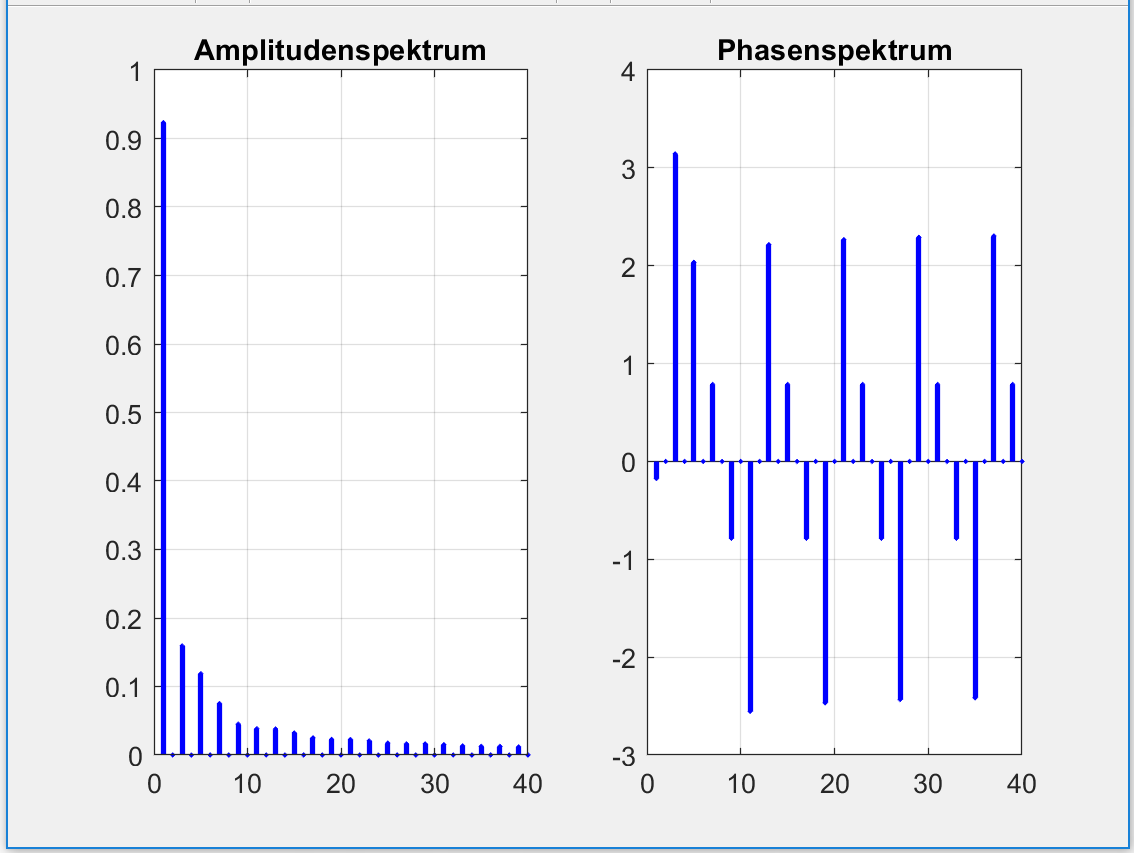
\includegraphics[width=0.4\linewidth]{A_PH_45.png}\label{fig:A_PH_45}}
	\caption{Phasenanschnittsteuerung mit 45\textdegree (a) Eingangssignal (b) Amplituden- und Phasenspektrum}
	\label{fig:Phasenanschnittsteuerung_mit_45}
\end{figure}

\begin{figure}[ht!]
	\centering
	\subfloat[][]{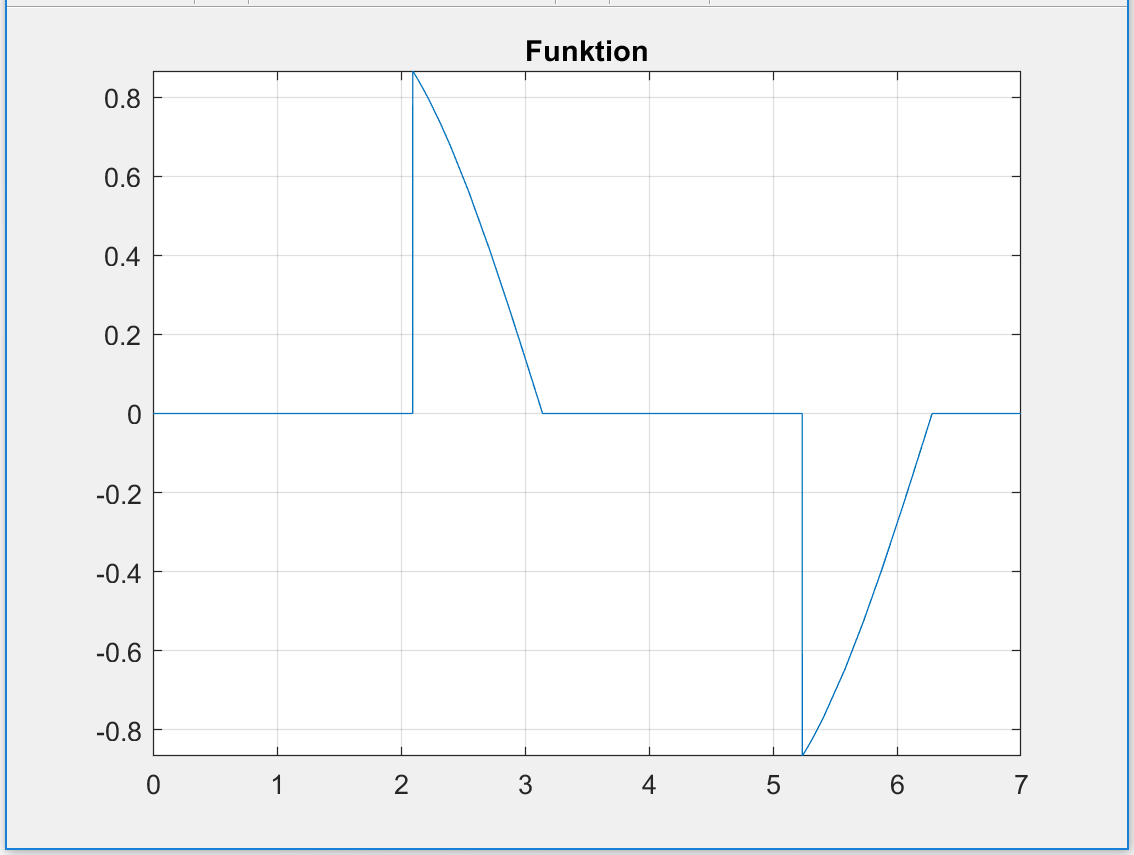
\includegraphics[width=0.4\linewidth]{eingangssignal_120.png}\label{fig:eingangssignal_120}}\qquad
	\subfloat[][]{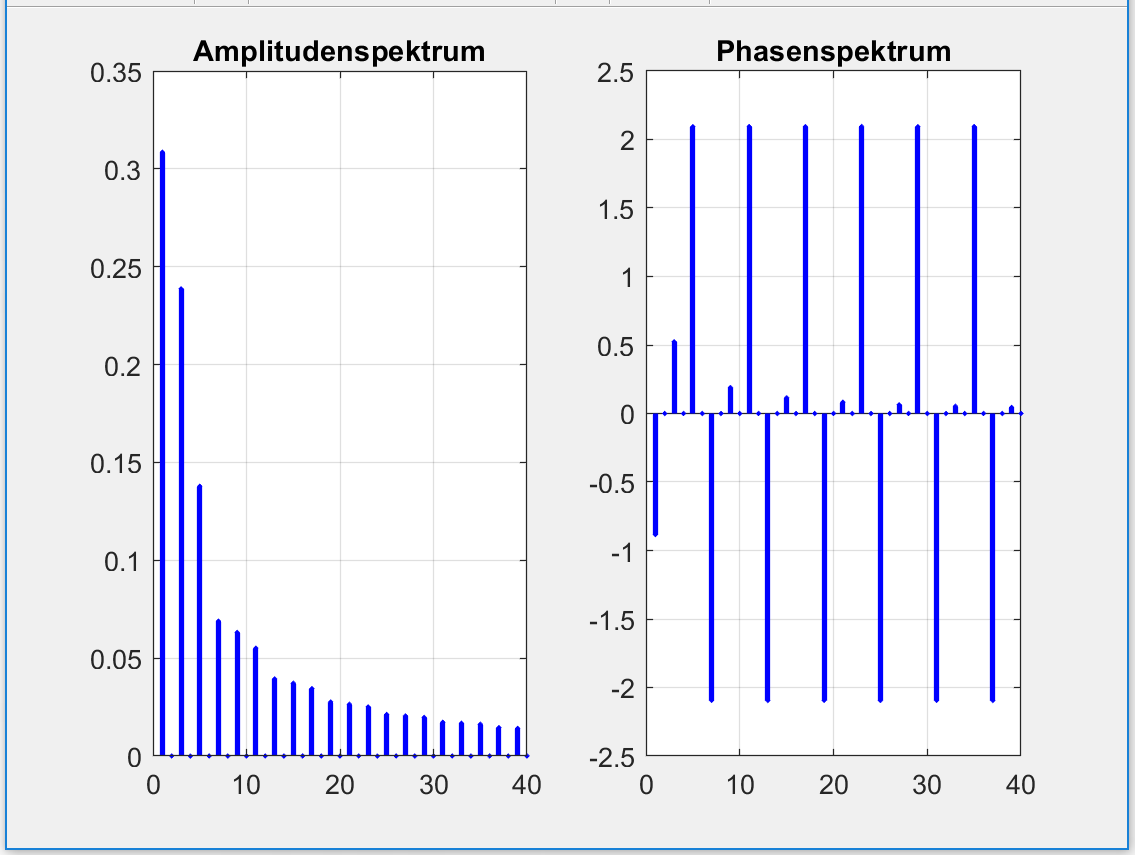
\includegraphics[width=0.4\linewidth]{A_PH_120.png}\label{fig:A_PH_120}}
	\caption{Phasenanschnittsteuerung mit 120\textdegree (a) Eingangssignal (b) Amplituden- und Phasenspektrum}
	\label{fig:Phasenanschnittsteuerung_mit_120}
\end{figure}

\newpage

\begin{figure}[ht!]
	\centering
	\subfloat[][]{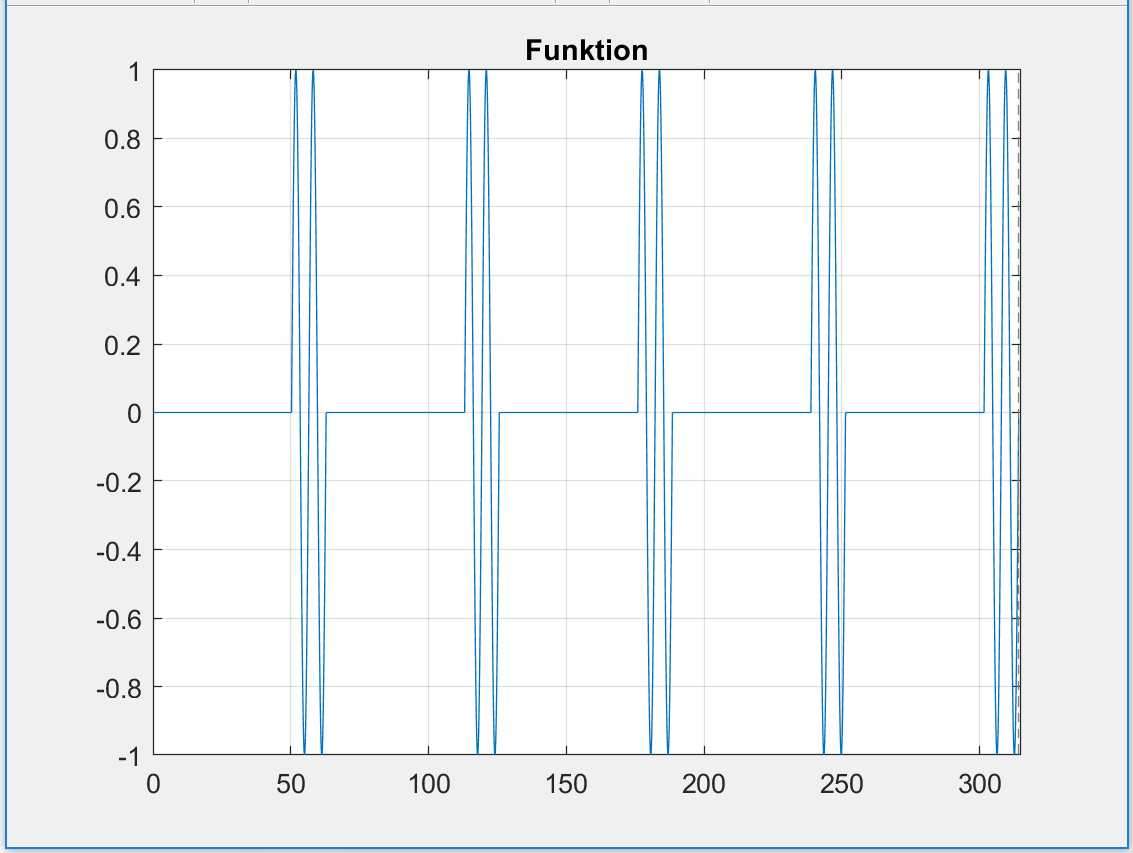
\includegraphics[width=0.4\linewidth]{Schwingungspaket_0_2.png}\label{fig:Schwingungspaket_0_2}}\qquad
	\subfloat[][]{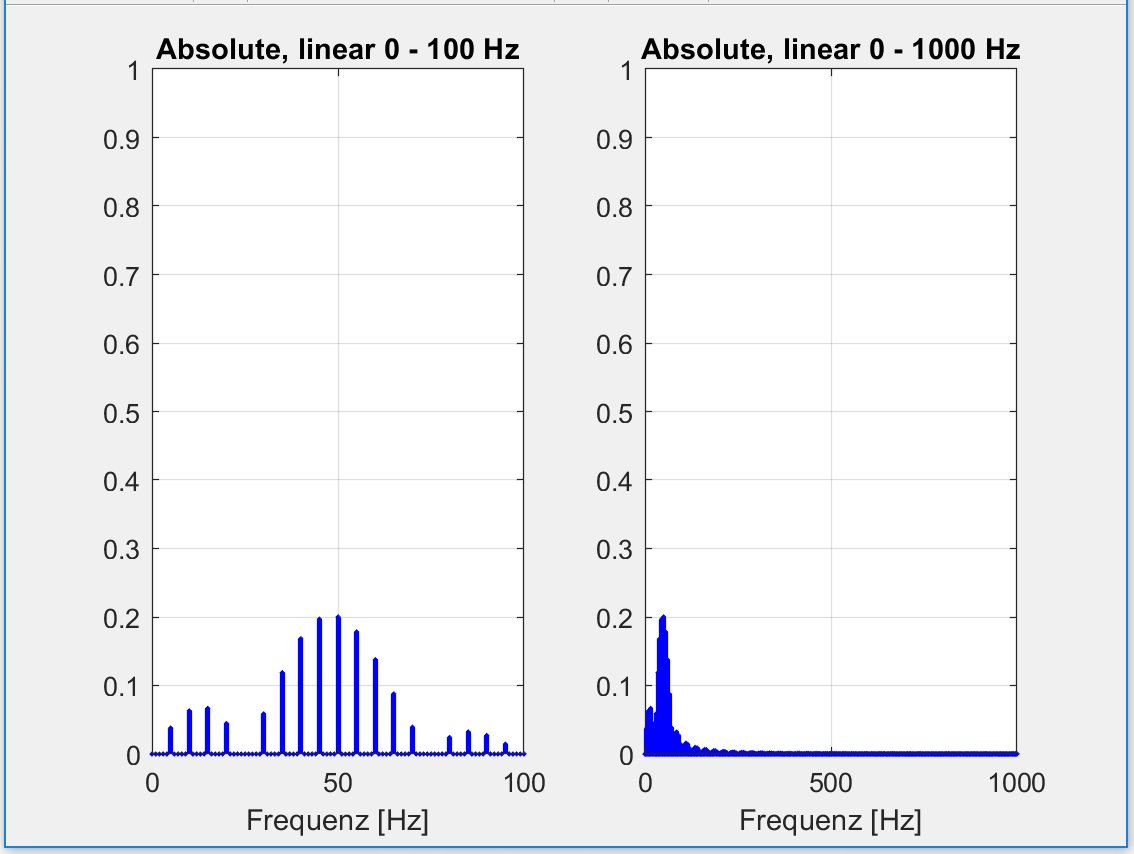
\includegraphics[width=0.4\linewidth]{Oberwellen_0_2.png}\label{fig:Oberwellen_0_2}}
	\caption{Schwingungspaket mit Duty Cycle 0.2 (a) Eingangssignal (b) Amplituden- und Phasenspektrum}
	\label{fig:Schwingungspaketsteuerung_mit_duty_cycle_0_2}
\end{figure}


\begin{figure}[ht!]
	\centering
	\subfloat[][]{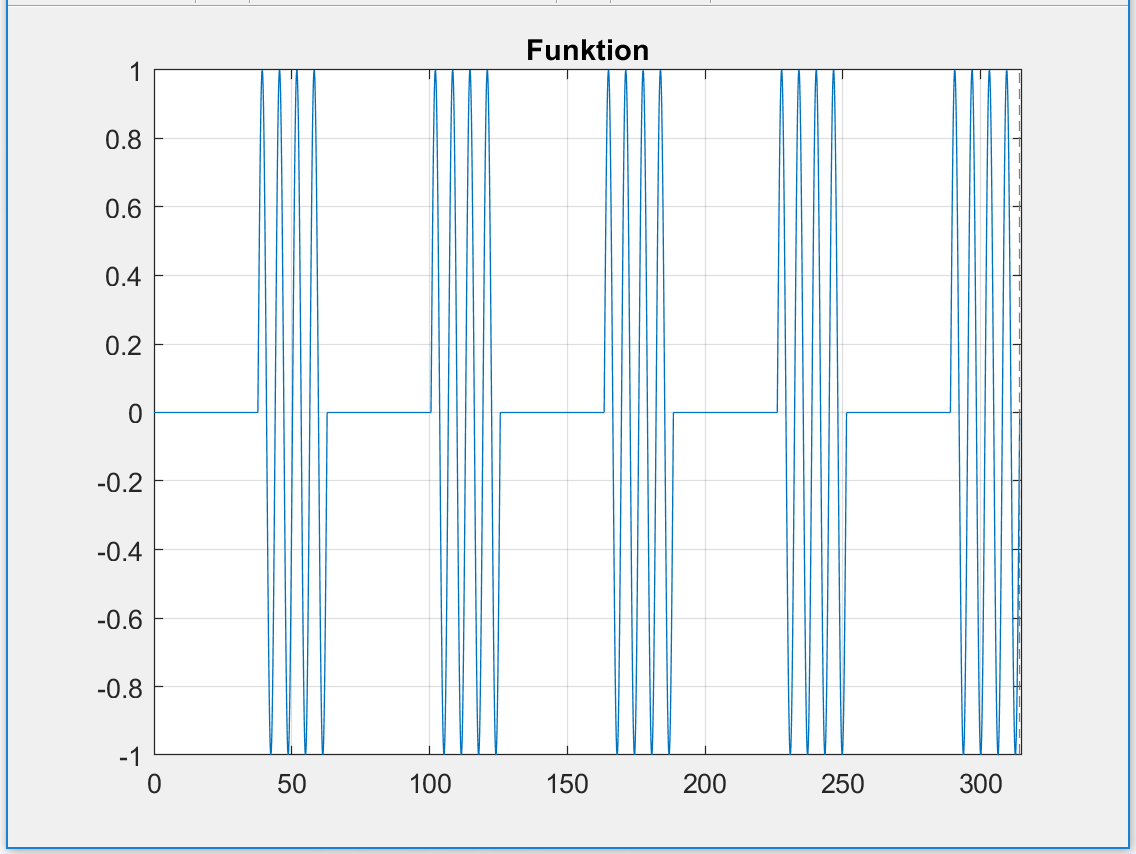
\includegraphics[width=0.4\linewidth]{Schwingungspaket_0_4.png}\label{fig:Schwingungspaket_0_4}}\qquad
	\subfloat[][]{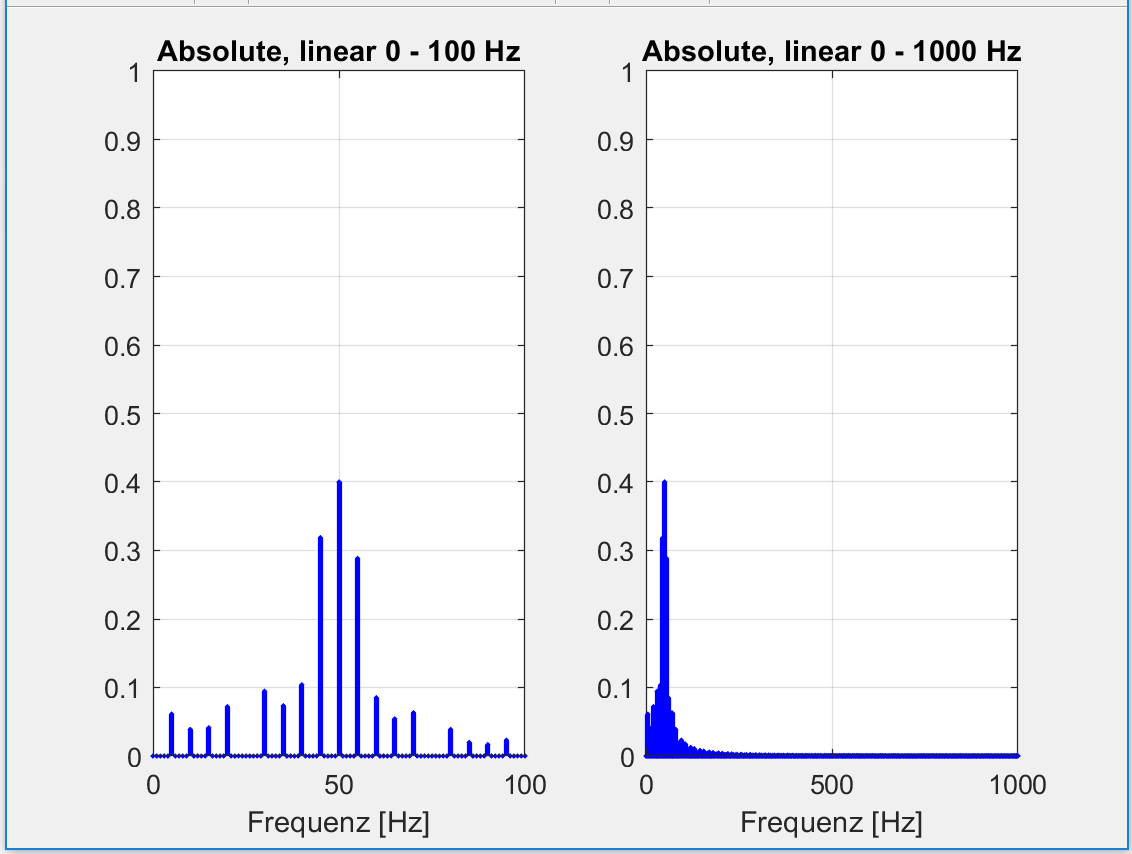
\includegraphics[width=0.4\linewidth]{Oberwellen_0_4.png}\label{fig:Oberwellen_0_4}}
	\caption{Schwingungspaket mit Duty Cycle 0.4 (a) Eingangssignal (b) Amplituden- und Phasenspektrum}
	\label{fig:Schwingungspaketsteuerung_mit_duty_cycle_0_4}
\end{figure}

\begin{figure}[ht!]
	\centering
	\subfloat[][]{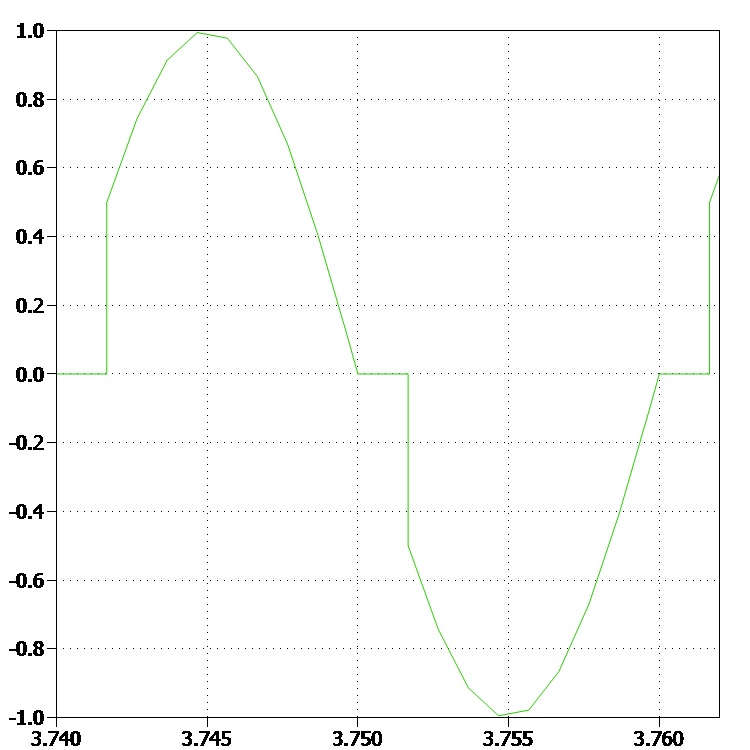
\includegraphics[width=0.32\linewidth]{plecs_phasenanschnitt_pi_6_funktion.png}\label{fig:plecs_phasenanschnitt_pi_6_funktion}}\qquad
	\subfloat[][]{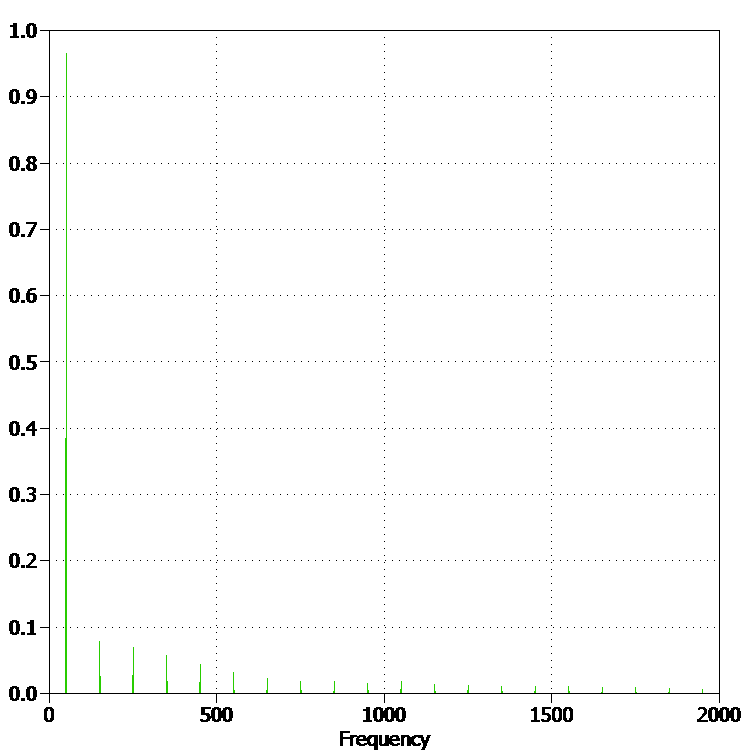
\includegraphics[width=0.32\linewidth]{plecs_phasenanschnitt_pi_6.png}\label{fig:plecs_phasenanschnitt_pi_6}}
	\caption{Phasenanschnitt mit 30\textdegree simuliert mit Plecs (a) Eingangssignal (b) Amplituden- und Phasenspektrum}
	\label{fig:Plecs_mit_phasenanschnitt_30}
\end{figure}

\newpage

\begin{figure}[ht!]
	\centering
	\subfloat[][]{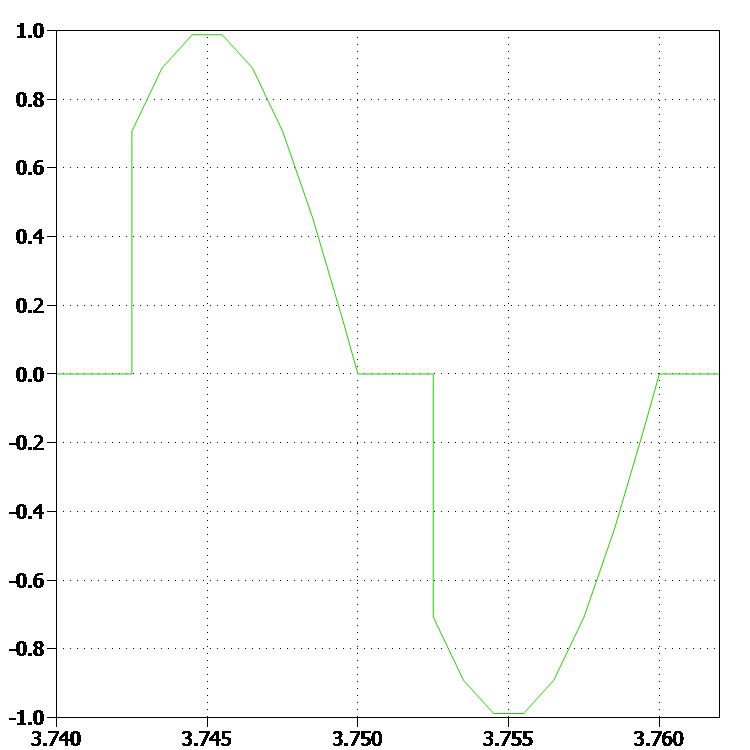
\includegraphics[width=0.32\linewidth]{plecs_phasenanschnitt_pi_4_funktion.png}\label{fig:plecs_phasenanschnitt_pi_4_funktion}}\qquad
	\subfloat[][]{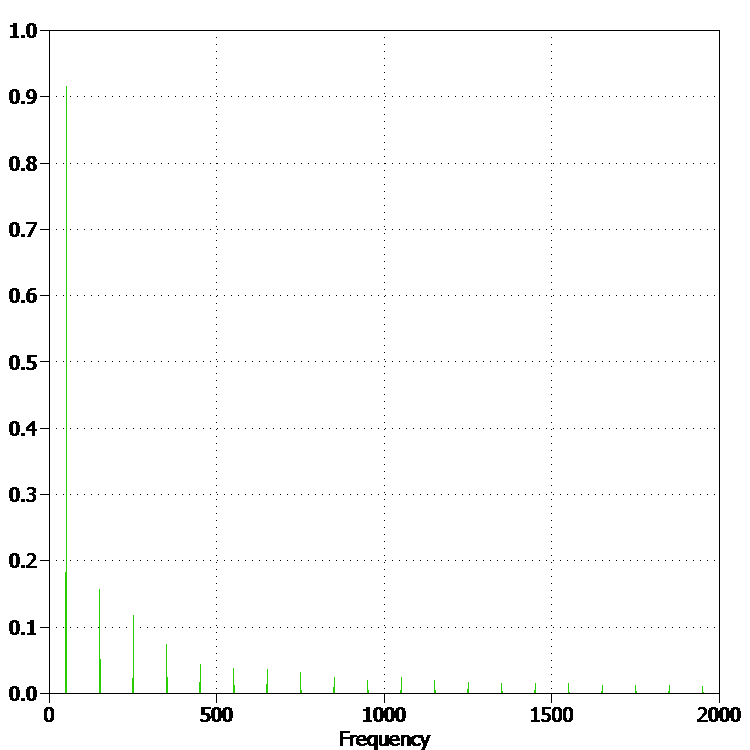
\includegraphics[width=0.32\linewidth]{plecs_phasenanschnitt_pi_4.png}\label{fig:plecs_phasenanschnitt_pi_4}}
	\caption{Phasenanschnitt mit 45\textdegree simuliert mit Plecs (a) Eingangssignal (b) Amplituden- und Phasenspektrum}
	\label{fig:Plecs_mit_phasenanschnitt_45}
\end{figure}


\begin{figure}[ht!]
	\centering
	\subfloat[][]{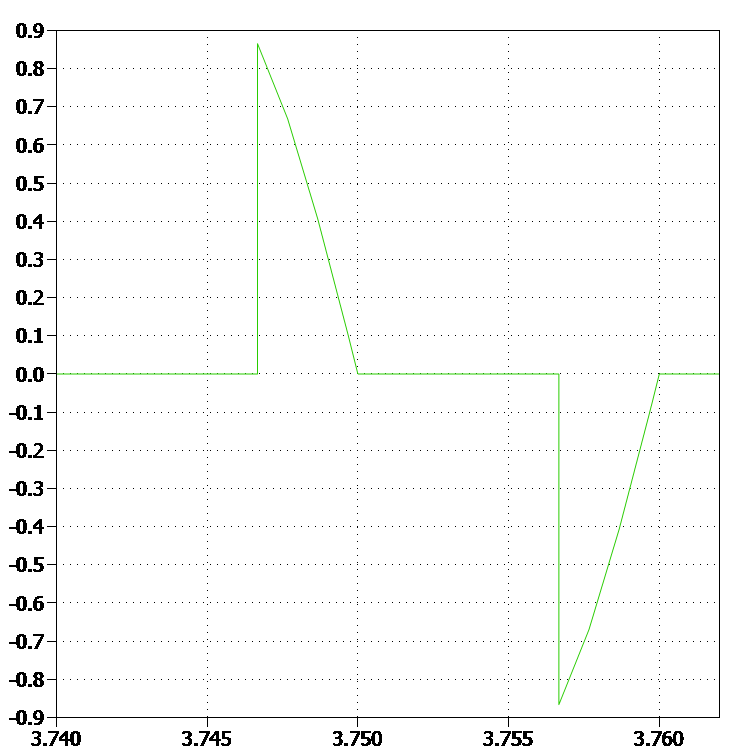
\includegraphics[width=0.32\linewidth]{plecs_phasenanschnitt_120_funktion.png}\label{fig:plecs_phasenanschnitt_120_funktion}}\qquad
	\subfloat[][]{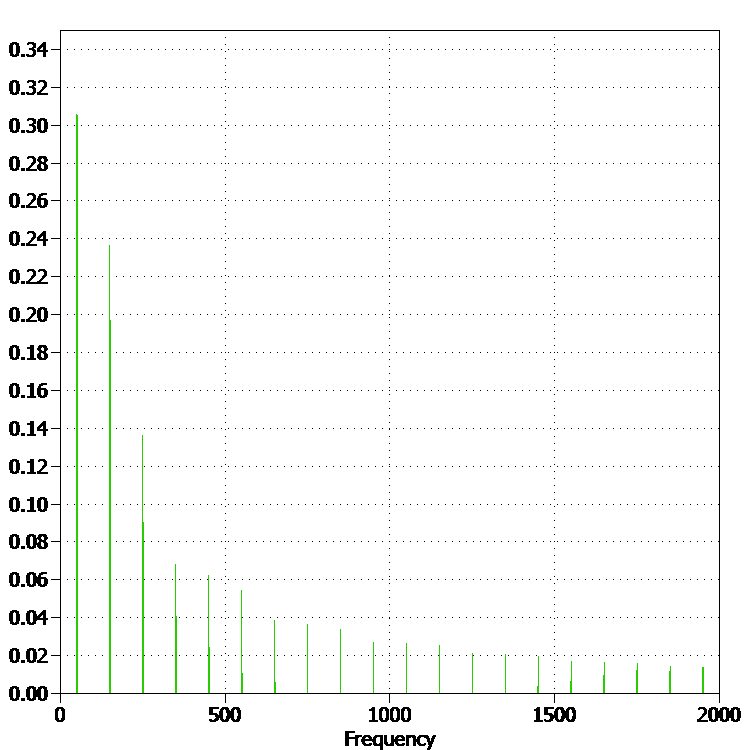
\includegraphics[width=0.32\linewidth]{plecs_phasenanschnitt_120.png}\label{fig:plecs_phasenanschnitt_120}}
	\caption{Phasenanschnitt mit 120\textdegree simuliert mit Plecs (a) Eingangssignal (b) Amplituden- und Phasenspektrum}
	\label{fig:Plecs_mit_phasenanschnitt_120}
\end{figure}


\begin{figure}[ht!]
	\centering
	\subfloat[][]{\includegraphics[width=0.32\linewidth]{plecs_schwingungspacket_0_2_schwingungen.PNG}\label{fig:plecs_schwingungspacket_0_2_schwingungen}}\qquad
	\subfloat[][]{\includegraphics[width=0.32\linewidth]{plecs_schwingungspacket_0_2_1000.PNG}\label{fig:plecs_schwingungspacket_0_2_1000}}
	\caption{Schwingungspaketsteuerung mit Duty Cycle 0.2 simuliert mit Plecs (a) Eingangssignal (b) Amplitudenspektrum}
	\label{fig:Schwingungspaketsteuerung_mit_duty_cycle_0_2 simuliert_mit_Plecs}
\end{figure}

\newpage

\begin{figure}[ht!]
	\centering
	\subfloat[][]{\includegraphics[width=0.32\linewidth]{plecs_schwingungspacket_0_4_schwingungen.PNG}\label{fig:plecs_schwingungspacket_0_4_schwingungen}}\qquad
	\subfloat[][]{\includegraphics[width=0.32\linewidth]{plecs_schwingungspacket_0_2_1000.PNG}\label{fig:plecs_schwingungspacket_0_4_1000}}
	\caption{Schwingungspaketsteuerung mit Duty Cycle 0.4 simuliert mit Plecs (a) Eingangssignal (b) Amplitudenspektrum}
	\label{fig:Schwingungspaketsteuerung_mit_duty_cycle_0_4 simuliert_mit_Plecs}
\end{figure}

\begin{figure}[ht!]  
	\centering 
	\includegraphics[scale=0.75]{Vergleich_Amplitudenspektrum_mit_Phasenwinkel_60.png}	
	\caption{Vergleich der Amplitudenspektrum mit Phasenwinkel von 60\textdegree}
	\label{fig:Vergleich_der_Amplitudenspektrum_mit Phasenwinkel_von_60}
\end{figure} 


\begin{figure}[ht!]
	\centering
	\includegraphics[scale=0.55]{Vergleich_einphasiges_Schwingungspaket_mit_duty_cycle_von_0_5.png}	
	\caption{Vergleich des Schwingungspaket mit Duty Cycle von 0.5}
	\label{fig:Vergleich des Schwingungspaket mit Duty Cycle von 0.5}
\end{figure}

\newpage

\begin{figure}[ht!]
	\centering
	\includegraphics[scale=0.55]{Vergleich_einphasiges_Schwingungspaket_mit_duty_cycle_von_0_8.png}	
	\caption{Vergleich des Schwingungspaket mit Duty Cycle von 0.8}
	\label{fig:Vergleich des Schwingungspaket mit Duty Cycle von 0.8}
\end{figure}

\begin{figure}[ht!]
	\centering
	\includegraphics[scale=0.55]{Vergleich_absolut_logarithmic_duty_cycle_von_0_5_mit_legende.PNG}	
	\caption{Vergleich der absolut logarithmische Werte des Schwingungspaket mit Duty Cycle von 0.8}
	\label{fig:Vergleich_absolut_logarithmic_duty_cycle_von_0_5_mit_legende}
\end{figure}

\begin{figure}[ht!]
	\centering
	\includegraphics[scale=0.55]{Vergleich_absolut_logarithmic_duty_cycle_von_0_8_mit_legende.PNG}	
	\caption{Vergleich der absolut logarithmische Werte des Schwingungspaket mit Duty Cycle von 0.8}
	\label{fig:Vergleich_absolut_logarithmic_duty_cycle_von_0_8_mit_legende}
\end{figure}

\begin{minipage}{0.49\textwidth}
	\centering
	\begin{tabular}{|l|l|l|}
		\hline
		Frequenz & Matlab  & Plecs     \\ \hline
		50       & 0.8392  & 0.832293  \\ \hline
		150      & 0.2387  & 0.236735  \\ \hline
		250      & 0.1378  & 0.136638  \\ \hline
		350      & 0.06892 & 0.0683341 \\ \hline
		450      & 0.06316 & 0.0625278 \\ \hline
		550      & 0.05513 & 0.0545493 \\ \hline
		650      & 0.03938 & 0.0389562 \\ \hline
		750      & 0.03716 & 0.0365021 \\ \hline
		850      & 0.03446 & 0.0336658 \\ \hline
		950      & 0.02757 & 0.0278878 \\ \hline
		1050     & 0.0264  & 0.0276274 \\ \hline
		1150     & 0.02506 & 0.0253678 \\ \hline
		1250     & 0.0212  & 0.0213567 \\ \hline
		1350     & 0.02049 & 0.0205108 \\ \hline
		1450     & 0.01969 & 0.0196758 \\ \hline
		1550     & 0.01723 & 0.0172034 \\ \hline
		1650     & 0.01675 & 0.0166963 \\ \hline
		1750     & 0.01622 & 0.0161076 \\ \hline
		1850     & 0.01451 & 0.0143616 \\ \hline
		1950     & 0.01416 & 0.0137444 \\ \hline
	\end{tabular}
\captionof{table}{Vergleich der Werte des Phasenanschnittes mit 60\textdegree}
\label{tab:Phas_60_Vergleich}
\end{minipage}
%
\begin{minipage}{0.49\textwidth}
	\begin{tabular}{|l|l|l|}
		\hline
		Frequenz & Matlab  & Plecs     \\ \hline
		50       & 0.5927  & 0.587846  \\ \hline
		150      & 0.3183  & 0.3157    \\ \hline
		250      & 0.1061  & 0.105158  \\ \hline
		350      & 0.1061  & 0.105196  \\ \hline
		450      & 0.06366 & 0.0630047 \\ \hline
		550      & 0.06366 & 0.0630497 \\ \hline
		650      & 0.04547 & 0.044839  \\ \hline
		750      & 0.04547 & 0.0449042 \\ \hline
		850      & 0.03537 & 0.0342252 \\ \hline
		950      & 0.03537 & 0.0344228 \\ \hline
		1050     & 0.02894 & 0.0296088 \\ \hline
		1150     & 0.02894 & 0.0294399 \\ \hline
		1250     & 0.02449 & 0.0245782 \\ \hline
		1350     & 0.02449 & 0.0245363 \\ \hline
		1450     & 0.02122 & 0.0212078 \\ \hline
		1550     & 0.02122 & 0.0211877 \\ \hline
		1650     & 0.01872 & 0.0186503 \\ \hline
		1750     & 0.01872 & 0.0186415 \\ \hline
		1850     & 0.01675 & 0.0165256 \\ \hline
		1950     & 0.01675 & 0.0165378 \\ \hline
	\end{tabular}
\captionof{table}{Vergleich der Werte des Phasenanschnittes mit 90\textdegree}
\label{tab:Phas_90_Vergleich}
\end{minipage}

\newpage
\begin{minipage}{0.49\textwidth}
	\centering
	\begin{tabular}{|l|l|l|}
		\hline
		Frequenz & Matlab  & Plecs     \\ \hline
		5        & 0.06431 & 0.0637753 \\ \hline
		15       & 0.06996 & 0.0693821 \\ \hline
		25       & 0.08488 & 0.0841842 \\ \hline
		35       & 0.1248  & 0.123802  \\ \hline
		45       & 0.3351  & 0.332314  \\ \hline
		50       & 0.5     & 0.495901  \\ \hline
		55       & 0.3032  & 0.30067   \\ \hline
		65       & 0.09226 & 0.09151   \\ \hline
		75       & 0.05093 & 0.0505147 \\ \hline
		85       & 0.03368 & 0.0334101 \\ \hline
		95       & 0.02439 & 0.0241942 \\ \hline
	\end{tabular}
	\captionof{table}{Vergleich der Werte des Schwingungspaketes mit einem Duty Cycle von 0.5}
	\label{tab:Schwing_50_Vergleich}
\end{minipage}
%
\begin{minipage}{0.49\textwidth}
	\begin{tabular}{|l|l|l|}
		\hline
		Frequenz & Matlab & Plecs    \\ \hline
		5        & -23.84 & -23.907  \\ \hline
		15       & -23.1  & -23.175  \\ \hline
		25       & -21.42 & -21.4954 \\ \hline
		35       & -18.07 & -18.1455 \\ \hline
		45       & -9.497 & -9.56903 \\ \hline
		50       & -6.021 & -6.0921  \\ \hline
		55       & -10.37 & -10.4382 \\ \hline
		65       & -20.7  & -20.7706 \\ \hline
		75       & -25.86 & -25.9316 \\ \hline
		85       & -29.45 & -29.5225 \\ \hline
		95       & -32.26 & -32.3258 \\ \hline
	\end{tabular}
	\captionof{table}{Vergleich der absolut logarithmische Werte des Schwingungspaketes mit einem Duty Cycle von 0.5}
	\label{tab:abs_Schwing_50_Vergleich} 	
\end{minipage}

\begin{minipage}{0.49\textwidth}
	\centering
	\begin{tabular}{|l|l|l|}
		\hline
		Frequenz & Matlab & Plecs    \\ \hline
		5        & -28.45 & -28.5226 \\ \hline
		10       & -24    & -24.0755 \\ \hline
		15       & -23.54 & -23.6109 \\ \hline
		20       & -27.02 & -27.0954 \\ \hline
		25       &        &          \\ \hline
		30       & -24.66 & -24.7333 \\ \hline
		35       & -18.51 & -18.5814 \\ \hline
		40       & -15.48 & -15.5559 \\ \hline
		45       & -14.11 & -14.1847 \\ \hline
		50       & -1.938 & -2.0097  \\ \hline
		55       & -14.98 & -15.0538 \\ \hline
		60       & -17.23 & -17.2987 \\ \hline
		65       & -21.14 & -21.2065 \\ \hline
		70       & -28.18 & -28.2546 \\ \hline
		75       &        &          \\ \hline
		80       & -32.4  & -32.4725 \\ \hline
		85       & -29.89 & -29.9583 \\ \hline
		90       & -31.36 & -31.4339 \\ \hline
		95       & -36.87 & -36.9414 \\ \hline
	\end{tabular}
	\captionof{table}{Vergleich der absolut logarithmische Werte des Schwingungspaketes mit einem Duty Cycle von 0.8}
	\label{tab:abs_Schwing_80_Vergleich}
\end{minipage}
%
\begin{minipage}{0.49\textwidth}
	\begin{tabular}{|l|l|l|}
		\hline
		Frequenz & Matlab  & Plecs     \\ \hline
		5        & 0.0378  & 0.0374862 \\ \hline
		10       & 0.06307 & 0.0625494 \\ \hline
		15       & 0.06653 & 0.0659863 \\ \hline
		20       & 0.04455 & 0.0441804 \\ \hline
		25       & 0       & 0         \\ \hline
		30       & 0.05847 & 0.0579873 \\ \hline
		35       & 0.1187  & 0.117742  \\ \hline
		40       & 0.1682  & 0.166803  \\ \hline
		45       & 0.1969  & 0.195329  \\ \hline
		50       & 0.8     & 0.793442  \\ \hline
		55       & 0.1782  & 0.176729  \\ \hline
		60       & 0.1376  & 0.136479  \\ \hline
		65       & 0.08775 & 0.0870312 \\ \hline
		70       & 0.03898 & 0.0386607 \\ \hline
		75       & 0       & 0         \\ \hline
		80       & 0.02399 & 0.0237918 \\ \hline
		85       & 0.03203 & 0.0317749 \\ \hline
		90       & 0.02703 & 0.0268104 \\ \hline
		95       & 0.01434 & 0.014221  \\ \hline
		100      & 0       & 0         \\ \hline
	\end{tabular}
\captionof{table}{Vergleich der Werte des des Schwingungspaketes mit einem Duty Cycle von 0.8}
\label{tab:Schwing_80_Vergleich}
\end{minipage}


\newpage
\section{Messungen}
\subsection{Messungen Spannungen Widerstand}\label{sec:Mess_Spannung_Widerstand}
\subsubsection*{Phasenanschnitt 60\textdegree}

\begin{figure}[ht!]
	\centering
	\includegraphics[width=0.96\textwidth]{Messung_Widerstand_Phas_60grad.png}	
	\caption{Messung mit Phasenanschnitt 60\textdegree}\label{fig:Mess_Phas_60}
\end{figure}

\subsubsection*{Phasenanschnitt 90\textdegree}
\begin{figure}[ht!]
	\centering
	\includegraphics[width=0.96\textwidth]{Messung_Widerstand_Phas_90grad.png}	
	\caption{Messung mit Phasenanschnitt 90\textdegree}\label{fig:Mess_Phas_90}
\end{figure}

\newpage
\subsection{Messungen Spannungen ASM}\label{sec:Mess_Spannung_ASM}
\subsubsection*{Schwingungspaket mit einem Duty Cycle von 0.5}
\begin{figure}[ht!]
	\centering
	\includegraphics[width=0.96\textwidth]{Messung_ASM_Schwing_0_5.png}	
	\caption{Messung mit Schwingungspaket mit einem Duty Cycle von 0.5}\label{fig:Mess_ASM_Schwing_0_5}
\end{figure}

\subsubsection*{Schwingungspaket mit einem Duty Cycle von 0.8}
\begin{figure}[ht!]
	\centering
	\includegraphics[width=0.96\textwidth]{Messung_ASM_Schwing_0_8.png}	
	\caption{Messung mit Schwingungspaket mit einem Duty Cycle von 0.8}\label{fig:Mess_ASM_Schwing_0_8}
\end{figure}
\newpage
\subsubsection*{Auf- und Absteuern}
\begin{figure}[ht!]
	\centering
	\includegraphics[width=0.96\textwidth]{Messung_ASM_Sanft.png}	
	\caption{Messung mit Sanft Anlasser}\label{fig:Mess_ASM_Sanft}
\end{figure}

\newpage
\subsection{Sparvariante für den Widerstand mit zwei Thyristoren} \label{sec:Sparvariante_2Thyristoren}
\subsubsection*{Phasenanschnitt 60\textdegree}

\begin{figure}[ht!]
	\centering
	\includegraphics[width=0.96\textwidth]{Mess_2Thyristoren_Widerstand_Phas_60.png}	
	\caption{Messung mit Phasenanschnitt 60\textdegree \hspace{0.02cm} und zwei Thyristoren}\label{fig:Mess_2Thyristoren_Phas_60grad}
\end{figure}

\subsubsection*{Phasenanschnitt 90\textdegree}

\begin{figure}[ht!]
	\centering
	\includegraphics[width=0.96\textwidth]{Mess_2Thyristoren_Widerstand_Phas_90.png}	
	\caption{Messung mit Phasenanschnitt 90\textdegree \hspace{0.02cm} und zwei Thyristoren}\label{fig:Mess_2Thyristoren_Phas_90grad}
\end{figure}

\newpage
\subsubsection*{Schwingungspaket mit einem Duty Cycle von 0.5}

\begin{figure}[ht!]
	\centering
	\includegraphics[width=0.96\textwidth]{Mess_2Thyristoren_Widerstand_Schwing_05.png}	
	\caption{Messung mit Schwingungspaket mit einem Duty Cycle von 0.5 und zwei Thyristoren}\label{fig:Mess_2Thyristoren_Schwing_50}
\end{figure}


\subsubsection*{Schwingungspaket mit einem Duty Cycle von 0.8}

\begin{figure}[ht!]
	\centering
	\includegraphics[width=0.96\textwidth]{Mess_2Thyristoren_Widerstand_Schwing_08.png}	
	\caption{Messung mit Schwingungspaket mit einem Duty Cycle von 0.8 und zwei Thyristoren}\label{fig:Mess_2Thyristoren_Schwing_80}	
\end{figure}

\newpage
\subsubsection*{Hartes Auf- und Absteuern}

\begin{figure}[ht!]
	\centering
	\includegraphics[width=0.96\textwidth]{Mess_2Thyristoren_Widerstand_AufAbFahren.png}	
	\caption{Messung mit dem harten Auf- und Absteuern und zwei Thyristoren}\label{Mess_2Thyristoren_Widerstand_AufAbFahren}	
\end{figure}


\begin{table}[ht!]
	\centering
	\begin{tabular}{|l|l|l|l|}
		\hline
		Frequenz {[}Hz{]} & Amplitude Phase 1 {[}V{]}                                                           & Amplitude Phase 2 {[}V{]}                                                           & Amplitude Phase 3 {[}V{]}                                                           \\ \hline
		49.65             & 68.8653                                                                             & 68.5665                                                                             & 57.1292                                                                             \\ \hline
		49.95             & 67.5597                                                                             & 50.5713                                                                             & 74.4293                                                                             \\ \hline
		50                & 142.7445                                                                            & 105.9402                                                                            & 157.2093                                                                            \\ \hline
		50.05             & 35.291                                                                              & 26.4882                                                                             & 38.8518                                                                             \\ \hline
		50.35             & 65.3531                                                                             & 65.6359                                                                             & 51.887                                                                              \\ \hline
		149.65            & 9.7876                                                                              & 2.7987                                                                              & 11.8526                                                                             \\ \hline
		150               & 8.3874                                                                              & 8.3817                                                                              & 7.6543                                                                              \\ \hline
		150.35            & 11.1326                                                                             & 2.5768                                                                              & 12.4114                                                                             \\ \hline \hline
		Frequenz {[}Hz{]} & \begin{tabular}[c]{@{}l@{}}Verhältnis zur \\ Grundschwingung\\ Phase 1\end{tabular} & \begin{tabular}[c]{@{}l@{}}Verhältnis zur \\ Grundschwingung\\ Phase 2\end{tabular} & \begin{tabular}[c]{@{}l@{}}Verhältnis zur \\ Grundschwingung\\ Phase 3\end{tabular} \\ \hline
		49.65             & 48.24\%                                                                             & 64.7\%                                                                              & 36.34\%                                                                             \\ \hline
		49.95             & 47.32\%                                                                             & 47.74\%                                                                             & 47.34\%                                                                             \\ \hline
		50                & 100\%                                                                               & 100\%                                                                               & 100\%                                                                               \\ \hline
		50.05             & 24.72\%                                                                             & 25\%                                                                                & 24.7\%                                                                              \\ \hline
		50.35             & 45.78\%                                                                             & 61.96\%                                                                             & 33\%                                                                                \\ \hline
		149.65            & 6.86\%                                                                              & 2.64\%                                                                              & 7.54\%                                                                              \\ \hline
		150               & 5.88\%                                                                              & 7.9\%                                                                               & 4.87\%                                                                              \\ \hline
		150.35            & 7.8\%                                                                               & 2.43\%                                                                              & 7.9\%                                                                               \\ \hline
	\end{tabular}
	\caption{Amplitudenwerte bei der Frequenzen mit zwei Thyristoren bei hartem Auf- und Absteuern}\label{tab:Mess_2Thyristoren_Spannung_Widerstand_AufAb_hart}
\end{table}

\newpage
\subsubsection{Sparvariante für die ASM mit zwei Thyristoren}

\subsubsection*{Sanftes Auf- und Absteuern}
\begin{figure}[ht!]
	\centering
	\includegraphics[width=0.96\textwidth]{Mess_ASM_2Thyristoren_AufAb_langsam.png}	
	\caption{Messung mit dem sanften Auf- und Absteuern und zwei Thyristoren}\label{fig:Mess_2Thyristoren_ASM_AufAbFahren_langsam}	
\end{figure}

\begin{table}[ht!]
	\centering
	\begin{tabular}{|l|l|l|l|}
		\hline
		Frequenz {[}Hz{]} & Amplitude Phase 1 {[}V{]}                                                           & Amplitude Phase 2 {[}V{]}                                                           & Amplitude Phase 3 {[}V{]}                                                           \\ \hline
		49.9              & 37.5857                                                                             & 42.9618                                                                             & 47.1945                                                                             \\ \hline
		49.95             & 75.5033                                                                             & 87.0174                                                                             & 77.0178                                                                             \\ \hline
		50                & 220.7586                                                                            & 216.2571                                                                            & 227.9957                                                                            \\ \hline
		50.05             & 111.631                                                                             & 110.0439                                                                            & 102.3768                                                                            \\ \hline
		50.1              & 44.4045                                                                             & 65.6359                                                                             & 40.8044                                                                             \\ \hline
		149.95            & 6.9369                                                                              & 2.1636                                                                              & 5.8686                                                                              \\ \hline
		150               & 11.5575                                                                             & 1.4866                                                                              & 10.115                                                                              \\ \hline
		150.05            & 6.7811                                                                              & 2.7637                                                                              & 6.5154                                                                              \\ \hline \hline
		Frequenz {[}Hz{]} & \begin{tabular}[c]{@{}l@{}}Verhältnis zur \\ Grundschwingung\\ Phase 1\end{tabular} & \begin{tabular}[c]{@{}l@{}}Verhältnis zur \\ Grundschwingung\\ Phase 2\end{tabular} & \begin{tabular}[c]{@{}l@{}}Verhältnis zur \\ Grundschwingung\\ Phase 3\end{tabular} \\ \hline
		49.9              & 17.03\%                                                                             & 19.46\%                                                                             & 20.7\%                                                                              \\ \hline
		49.95             & 34.2\%                                                                              & 39.42\%                                                                             & 33.78\%                                                                             \\ \hline
		50                & 100\%                                                                               & 100\%                                                                               & 100\%                                                                               \\ \hline
		50.05             & 50.57\%                                                                             & 49.85\%                                                                             & 44.9\%                                                                              \\ \hline
		50.1              & 20.11\%                                                                             & 29.73\%                                                                             & 17.9\%                                                                              \\ \hline
		149.95            & 3.16\%                                                                              & 0.98\%                                                                              & 2.57\%                                                                              \\ \hline
		150               & 5.24\%                                                                              & 0.67\%                                                                              & 4.44\%                                                                              \\ \hline
		150.05            & 3.07\%                                                                              & 1.25\%                                                                              & 2.86\%                                                                              \\ \hline
	\end{tabular}
	\caption{Amplitudenwerte bei der Frequenzen mit zwei Thyristoren bei sanftem Auf- und Absteuern}\label{tab:Mess_2Thyristoren_Spannung_ASM_AufAb_sanft}
\end{table}

\newpage
\subsection{Sparvariante für den Widerstand mit einem Thyristor} \label{sec:Sparvariante_1Thyristor}
\subsubsection*{Phasenanschnitt 60\textdegree}

\begin{figure}[ht]
	\centering
	\includegraphics[width=0.96\textwidth]{Mess_1Thyristor_Widerstand_Phas60.png}	
	\caption{Messung mit Phasenanschnitt 60\textdegree \hspace{0.02cm} und einem Thyristoren}\label{fig:Mess_1Thyristor_Phas_60grad}
\end{figure}


\subsubsection*{Phasenanschnitt 90\textdegree}

\begin{figure}[ht]
	\centering
	\includegraphics[width=0.96\textwidth]{Mess_1Thyristor_Widerstand_Phas90.png}	
	\caption{Messung mit Phasenanschnitt 90\textdegree \hspace{0.02cm} und einem Thyristoren}\label{fig:Mess_1Thyristor_Phas_90grad}
\end{figure}

\newpage
\subsubsection*{Schwingungspaket mit einem Duty Cycle von 0.5}

\begin{figure}[ht]
	\centering
	\includegraphics[width=0.9\textwidth]{Mess_1Thyristor_Widerstand_Schwing_05.png}	
	\caption{Messung mit Schwingungspaket mit einem Duty Cycle von 0.5 und einem Thyristoren}\label{fig:Mess_1Thyristor_Schwing_50}
\end{figure}

\subsubsection*{Schwingungspaket mit einem Duty Cycle von 0.8}

\begin{figure}[ht]
	\centering
	\includegraphics[width=0.9\textwidth]{Mess_1Thyristor_Widerstand_Schwing_08.png}	
	\caption{Messung mit Schwingungspaket mit einem Duty Cycle von 0.8 und einem Thyristoren}\label{fig:Mess_1Thyristoren_Schwing_80}	
\end{figure}

\newpage
\subsubsection*{Auf- und Absteuern}

\begin{figure}[ht]
	\centering
	\includegraphics[width=0.9\textwidth]{Mess_1Thyristor_Widerstand_AufAb.png}	
	\caption{Messung mit Auf- und Absteuern und einem Thyristoren}\label{Mess_1Thyristoren_Widerstand_AufAbFahren}	
\end{figure}


\subsubsection*{Langsames Auf- und Absteuern}

\begin{figure}[ht]
	\centering
	\includegraphics[width=0.9\textwidth]{Mess_1Thyristor_Widerstand_AufAb_langsam.png}	
	\caption{Messung mit dem langsamen Auf- und Absteuern und einem Thyristoren}\label{Mess_1Thyristoren_Widerstand_AufAbFahren_langsam}	
\end{figure}

\newpage
\subsection{Vergleich Messungen Widerstand mit Simulation}
\subsubsection*{Schwingungspaket mit einem Duty Cycle von 0.5} \label{sec:Vergleich_Mess_Sim_Schwing_50}

\begin{figure}[ht!]
	\begin{minipage}[b]{0.59\textwidth}
		\centering
		\includegraphics[width=\textwidth]{Vergleich_Mess_Sim_Schwing_50.png}	
		\caption{Vergleich Messung und Simulation mit Schwingungspaket mit einem Duty Cycle von 0.5}\label{fig:Vergleich_Schwing_50}
	\end{minipage}
	%
	\begin{minipage}[b]{0.4\textwidth}
		\centering
		\begin{tabular}{|l|l|l|}
			\hline
			\begin{tabular}[c]{@{}l@{}}Fre-\\ quenz\\ {[}Hz{]}\end{tabular} & \begin{tabular}[c]{@{}l@{}}Simu-\\ lation\\ {[}V{]}\end{tabular} & \begin{tabular}[c]{@{}l@{}}Mes\\ sung\\ {[}V{]}\end{tabular} \\ \hline
			46                                                              & 1.676                                                            & 14.735                                                       \\ \hline
			47                                                              & 35.352                                                           & 28                                                           \\ \hline
			48                                                              & 1.667                                                            & 26.376                                                       \\ \hline
			49                                                              & 102.412                                                          & 95.6                                                         \\ \hline
			50                                                              & 161.597                                                          & 149.92                                                       \\ \hline
			51                                                              & 101.858                                                          & 99.8                                                         \\ \hline
			52                                                              & 1.648                                                            & 25.134                                                       \\ \hline
			53                                                              & 33.293                                                           & 20.6                                                         \\ \hline
		\end{tabular}
		\caption{Vergleich Messung und Simulation mit Schwingungspaket mit einem Duty Cycle von 0.5}\label{tab:Vergleich_Schwing_50}
	\end{minipage}
\end{figure}


\subsubsection*{Schwingungspaket mit einem Duty Cycle von 0.8} \label{sec:Vergleich_Mess_Sim_Schwing_80}
\begin{figure}[ht!]
	\begin{minipage}[b]{0.59\textwidth}
		\centering
		\includegraphics[width=\textwidth]{Vergleich_Mess_Sim_Schwing_80.png}	
		\caption{Vergleich Messung und Simulation mit Schwingungspaket mit einem Duty Cycle von 0.8}\label{fig:Vergleich_Schwing_80}
	\end{minipage}
	%
	\begin{minipage}[b]{0.4\textwidth}
		\centering
		\begin{tabular}{|l|l|l|}
			\hline
			\begin{tabular}[c]{@{}l@{}}Fre-\\ quenz\\ {[}Hz{]}\end{tabular} & \begin{tabular}[c]{@{}l@{}}Simu-\\ lation\\ {[}V{]}\end{tabular} & \begin{tabular}[c]{@{}l@{}}Mes\\ sung\\ {[}V{]}\end{tabular} \\ \hline
			46                                                              & 16.335                                                           & 20.173                                                       \\ \hline
			47                                                              & 32.649                                                           & 28.26                                                        \\ \hline
			48                                                              & 47.944                                                           & 40.576                                                       \\ \hline
			49                                                              & 61.08                                                            & 62.694                                                       \\ \hline
			50                                                              & 260.212                                                          & 265.98                                                       \\ \hline
			51                                                              & 59.54                                                            & 65.7                                                         \\ \hline
			52                                                              & 47.781                                                           & 43.812                                                       \\ \hline
			53                                                              & 31.664                                                           & 21.939                                                       \\ \hline
		\end{tabular}
		\caption{Vergleich Messung und Simulation mit Schwingungspaket mit einem Duty Cycle von 0.8}\label{tab:Vergleich_Schwing_80}
	\end{minipage}
\end{figure}



\newpage
\subsubsection*{Hartes Auf- und Absteuern}\label{sec:Vergleich_Mess_Sim_hart_AufAb}
\begin{figure}[ht!]
	\begin{minipage}[b]{0.59\textwidth}
		\centering
		\includegraphics[width=\textwidth]{Vergleich_Mess_Sim_hart_AufAb.png}	
		\caption{Vergleich Messung und Simulation mit hartem Auf- und Absteuern}\label{fig:Vergleich_hart_AufAb}
	\end{minipage}
	%
	\begin{minipage}[b]{0.4\textwidth}
		\centering
		\begin{tabular}{|l|l|l|}
			\hline
			\begin{tabular}[c]{@{}l@{}}Fre-\\ quenz\\ {[}Hz{]}\end{tabular} & \begin{tabular}[c]{@{}l@{}}Simu-\\ lation\\ {[}V{]}\end{tabular} & \begin{tabular}[c]{@{}l@{}}Mes-\\ sung\\ {[}V{]}\end{tabular} \\ \hline
			49.65                                                           & 22.167                                                           & 67.126                                                        \\ \hline
			49.7                                                            & 24.504                                                           & 40.959                                                        \\ \hline
			50                                                              & 145.271                                                          & 11.676                                                        \\ \hline
			50.05                                                           & 55.113                                                           & 58.202                                                        \\ \hline
			50.35                                                           & 22.2                                                             & 70.065                                                        \\ \hline
			249                                                             & 0.473                                                            & 9.03                                                          \\ \hline
			250                                                             & 1.157                                                            & 0.108                                                         \\ \hline
			251                                                             & 0.29021                                                          & 1.53                                                          \\ \hline
		\end{tabular}
		\caption{Vergleich Messung und Simulation mit hartem Auf- und Absteuern}\label{tab:Vergleich_hart_AufAb}
	\end{minipage}
\end{figure}


\subsubsection*{Sanftes Auf- und Absteuern}\label{sec:Vergleich_Mess_Sim_sanft_AufAb}
\begin{figure}[ht!]
	\begin{minipage}[b]{0.59\textwidth}
		\centering
		\includegraphics[width=\textwidth]{Vergleich_Mess_Sim_sanft_AufAb.png}	
		\caption{Vergleich Messung und Simulation mit sanftem Auf- und Absteuern}\label{fig:Vergleich_sanft_AufAb}
	\end{minipage}
	%
	\begin{minipage}[b]{0.4\textwidth}
		\centering
		\begin{tabular}{|l|l|l|}
			\hline
			\begin{tabular}[c]{@{}l@{}}Fre-\\ quenz\\ {[}Hz{]}\end{tabular} & \begin{tabular}[c]{@{}l@{}}Simu-\\ lation\\ {[}V{]}\end{tabular} & \begin{tabular}[c]{@{}l@{}}Mes-\\ sung\\ {[}V{]}\end{tabular} \\ \hline
			49.8               & 66.953             & 18.522          \\ \hline
			49.85              & 24.870             & 26.576          \\ \hline
			49.9               & 174.378            & 29.507          \\ \hline
			49.95              & 314.127            & 91.266          \\ \hline
			50                 & 370.962            & 172.241         \\ \hline
			50.05              & 314.051            & 116.719         \\ \hline
			50.1               & 174.266            & 28.629          \\ \hline
			50.15              & 24.871             & 30.076          \\ \hline
			50.2               & 66.83              & 18.72           \\ \hline
			249.6              & 0.188              & 8.158           \\ \hline
			250                & 0.4967             & 1.158           \\ \hline
			250.4              & 0.445              & 7.466           \\ \hline
		\end{tabular}
		\caption{Vergleich Messung und Simulation mit sanftem Auf- und Absteuern}\label{tab:Vergleich_sanft_AufAb}
	\end{minipage}
\end{figure}


\end{appendix}




%%---NOTES for DEBUG---------------------------------------------------------------------
\ifdraft{%Do this only if mode=draft
%%requires \usepackage{todonotes})
\newpage
%\listoftodos[\section{Todo-Notes}]
\clearpage
}
{%Do this only if mode=final
}
\end{document}
